%!TEX TS-program = xelatex
\documentclass[10pt, compress]{beamer}

\usetheme[usetitleprogressbar]{m}

\usepackage{booktabs}
\usepackage{tikz}
\usepackage{dcolumn}
\usepackage[scale=2]{ccicons}
\usepackage{color}

\graphicspath{{Graphics/}}

\title[Tensors]{\textsc{Relax, Tensors Are Here...with Exogenous Covariates}}
\author[Hoff, Minhas, \& Ward]{Peter D. Hoff, Shahryar Minhas, \& Michael D. Ward} 
\date{\today}

\begin{document}
\frame{\titlepage}

%%%%%%%%%%%%%%%%%%%%%%%%%%%%%%%%%%%%%%%%%%%%%%%%%%%%%%%%%%%%
\frame
{
  \frametitle{Model Specification}
  \vspace{-5mm}
  \begin{itemize}
  \item Dependent variables: Log(Exports) and Stdzed(Material Conflict). 
  \item Direct ($i$), reciprocal ($ji$) and transitive ($ijk$) 1 month lags of these included as IVs.
  \item Exogenous Covariates:
    \begin{itemize}
    \item Number of Preferential Trade Agreements (PTA) between $i$ and $j$ (this is an undirected, yearly level variable). Direct and transitive version of this variable included as covariates.
    \item Presence of a defensive alliance relationship between $i$ and $j$ (undirected, yearly level). Direct and transitive versions.
    \item Centroid distance between $i$ and $j$ (directed). Direct version.
    \item Polity, monthly level variable. Polity of sender included.
    \item Log(GDP), yearly level variable but imputed at the monthly level. GDP of sender.
    \item Log(Population), yearly level variable but imputed at the monthly level. Population of sender.
    \item Log(Total Exports to any country), monthly level variable. Exports of sender.
    \end{itemize}
  \end{itemize}    
} 
%%%%%%%%%%%%%%%%%%%%%%%%%%%%%%%%%%%%%%%%%%%%%%%%%%%%%%%%%%%%

%%%%%%%%%%%%%%%%%%%%%%%%%%%%%%%%%%%%%%%%%%%%%%%%%%%%%%%%%%%%
\frame
{
  \frametitle{Sample \& Data}
  \begin{itemize}
  \item  Our sample is comprised of 161 countries over the period of March 2001 to December 2014
  \item Data sources:
  \begin{itemize}
    \item Exports: \href{http://data.imf.org/?sk=8aa6eb7c-598b-4d3b-82f4-adab95d23145&dsId=DS_1414779485682}{\textcolor{blue}{IMF Direction of Trade Statistics}}
    \item Material Conflict: ICEWS
    \item PTA: \href{http://www.designoftradeagreements.org/}{\textcolor{blue}{Design of Trade Agreements Database}}
    \item Alliance: \href{http://www.correlatesofwar.org/news/alliances-data-set-v4-1-available-1}{\textcolor{blue}{Correlates of War}}
    \item Distance: \href{http://nils.weidmann.ws/projects/cshapes}{\textcolor{blue}{cshapes}}
    \item Polity: \href{http://www.systemicpeace.org/polity/polity4.htm}{\textcolor{blue}{Polity IV Project}}
    \item GDP, Population: \href{https://www.imf.org/external/pubs/ft/weo/2014/02/weodata/index.aspx}{\textcolor{blue}{IMF World Economic Outlook Database}}
  \end{itemize}
  \end{itemize}    
} 
%%%%%%%%%%%%%%%%%%%%%%%%%%%%%%%%%%%%%%%%%%%%%%%%%%%%%%%%%%%%

%%%%%%%%%%%%%%%%%%%%%%%%%%%%%%%%%%%%%%%%%%%%%%%%%%%%%%%%%%%%
\frame
{
  \frametitle{Modeling Approach}
  \begin{itemize}
  \item Multilinear tensor regression framework
  \item MCMC run for 1300 iterations with first 600 used as burn-in\footnote{Using this many datapoints takes time the MCMC will keep running for another 3700 iterations so these results are preliminary, but trace plots at the end of this pdf look stable after 600 iterations}
  \item The model has the following form:
  \begin{align*}
  \textbf{Y} = \textbf{X} \times \{\boldsymbol{\beta_{1}}, \boldsymbol{\beta_{2}}, \boldsymbol{\beta_{3}} \} + \textbf{E}
  \end{align*}
  \item \textbf{Y} is a $161 \times 161 \times 2 \times 165$ array
  \item \textbf{X} is a $161 \times 161 \times 13 \times 165$ array, where each of the 13 variables is lagged by one month
  \end{itemize}    
} 
%%%%%%%%%%%%%%%%%%%%%%%%%%%%%%%%%%%%%%%%%%%%%%%%%%%%%%%%%%%%

%%%%%%%%%%%%%%%%%%%%%%%%%%%%%%%%%%%%%%%%%%%%%%%%%%%%%%%%%%%%
\frame
{
\frametitle{$\boldsymbol{\beta_{1}}$ \& $\boldsymbol{\beta_{2}}$, Sig. $+$ shown, $\alpha = 0.01$}
  \vspace{-15mm}
  \begin{figure}[ht]
  \centering
    \begin{tabular}{c}
      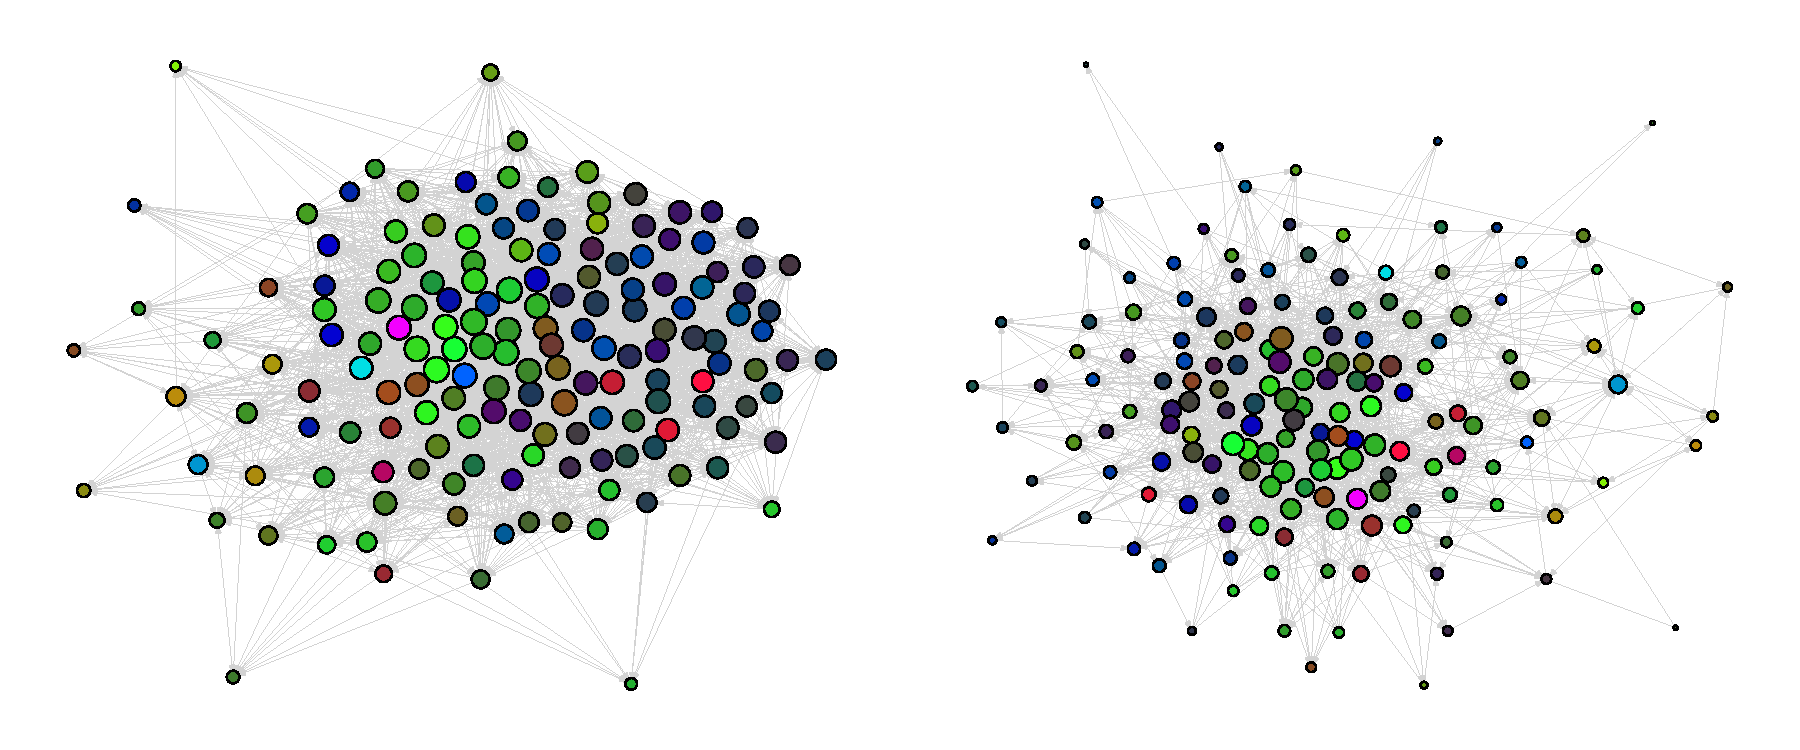
\includegraphics[width=1\textwidth]{net.pdf} \\
      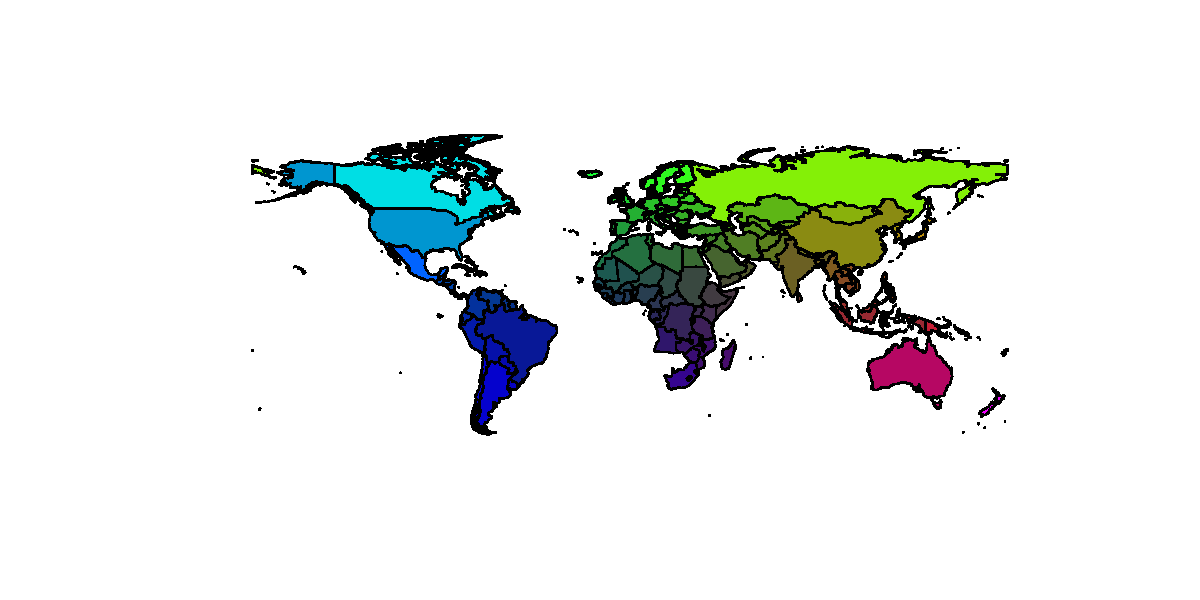
\includegraphics[width=.9\textwidth]{map.pdf}
    \end{tabular}
  \end{figure}
}
%%%%%%%%%%%%%%%%%%%%%%%%%%%%%%%%%%%%%%%%%%%%%%%%%%%%%%%%%%%%

%%%%%%%%%%%%%%%%%%%%%%%%%%%%%%%%%%%%%%%%%%%%%%%%%%%%%%%%%%%%
\frame
{
\frametitle{$\boldsymbol{\beta_{3}}$}
  \centering
  \resizebox{1\textwidth}{!}{% Created by tikzDevice version 0.8.1 on 2015-06-28 20:26:01
% !TEX encoding = UTF-8 Unicode
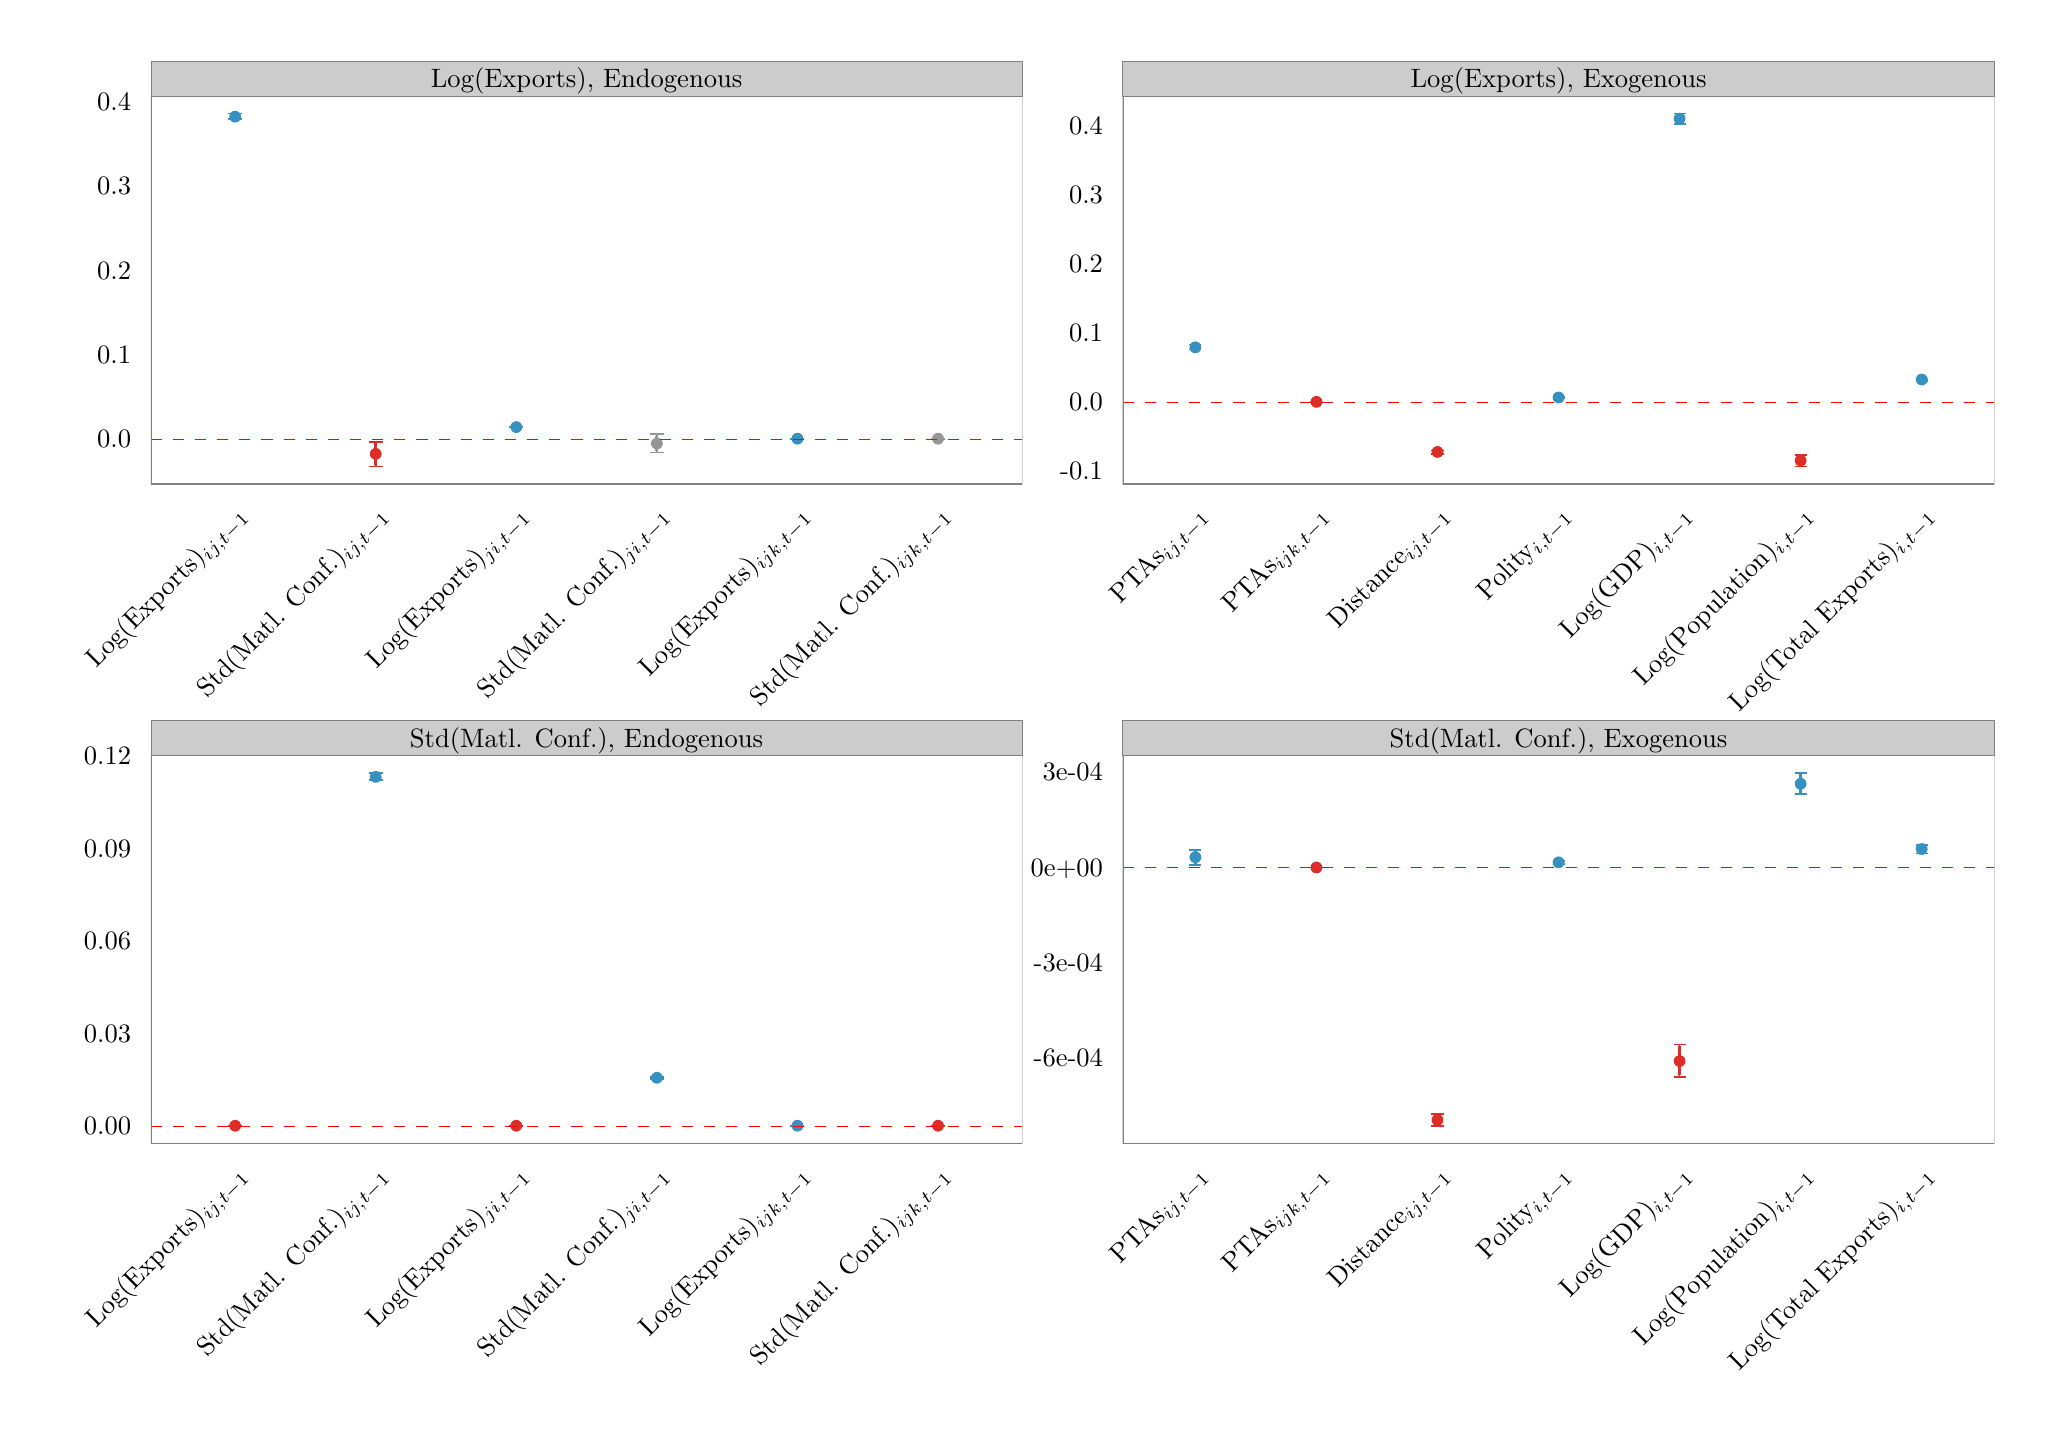
\begin{tikzpicture}[x=1pt,y=1pt]
\definecolor{fillColor}{RGB}{255,255,255}
\path[use as bounding box,fill=fillColor,fill opacity=0.00] (0,0) rectangle (722.70,505.89);
\begin{scope}
\path[clip] (  0.00,  0.00) rectangle (722.70,505.89);
\definecolor{drawColor}{RGB}{255,255,255}
\definecolor{fillColor}{RGB}{255,255,255}

\path[draw=drawColor,line width= 0.6pt,line join=round,line cap=round,fill=fillColor] (  0.00,  0.00) rectangle (722.70,505.89);
\end{scope}
\begin{scope}
\path[clip] ( 44.49,340.99) rectangle (359.44,481.21);
\definecolor{fillColor}{RGB}{54,144,192}

\path[fill=fillColor] ( 74.97,473.73) circle (  2.13);
\definecolor{fillColor}{RGB}{222,45,38}

\path[fill=fillColor] (125.77,351.89) circle (  2.13);
\definecolor{fillColor}{RGB}{54,144,192}

\path[fill=fillColor] (176.56,361.55) circle (  2.13);
\definecolor{fillColor}{gray}{0.59}

\path[fill=fillColor] (227.36,355.63) circle (  2.13);
\definecolor{fillColor}{RGB}{54,144,192}

\path[fill=fillColor] (278.16,357.36) circle (  2.13);
\definecolor{fillColor}{gray}{0.59}

\path[fill=fillColor] (328.96,357.36) circle (  2.13);
\definecolor{drawColor}{RGB}{54,144,192}

\path[draw=drawColor,draw opacity=0.30,line width= 0.3pt,line join=round] ( 74.97,472.79) -- ( 74.97,474.84);
\definecolor{drawColor}{RGB}{222,45,38}

\path[draw=drawColor,draw opacity=0.30,line width= 0.3pt,line join=round] (125.77,347.36) -- (125.77,356.18);
\definecolor{drawColor}{RGB}{54,144,192}

\path[draw=drawColor,draw opacity=0.30,line width= 0.3pt,line join=round] (176.56,361.43) -- (176.56,361.67);
\definecolor{drawColor}{RGB}{150,150,150}

\path[draw=drawColor,draw opacity=0.30,line width= 0.3pt,line join=round] (227.36,352.41) -- (227.36,359.04);
\definecolor{drawColor}{RGB}{54,144,192}

\path[draw=drawColor,draw opacity=0.30,line width= 0.3pt,line join=round] (278.16,357.36) -- (278.16,357.36);
\definecolor{drawColor}{RGB}{150,150,150}

\path[draw=drawColor,draw opacity=0.30,line width= 0.3pt,line join=round] (328.96,357.35) -- (328.96,357.37);
\definecolor{drawColor}{RGB}{54,144,192}

\path[draw=drawColor,line width= 1.1pt,line join=round] ( 74.97,472.86) -- ( 74.97,474.75);
\definecolor{drawColor}{RGB}{222,45,38}

\path[draw=drawColor,line width= 1.1pt,line join=round] (125.77,347.76) -- (125.77,355.64);
\definecolor{drawColor}{RGB}{54,144,192}

\path[draw=drawColor,line width= 1.1pt,line join=round] (176.56,361.45) -- (176.56,361.66);
\definecolor{drawColor}{gray}{0.59}

\path[draw=drawColor,line width= 1.1pt,line join=round] (227.36,352.95) -- (227.36,358.31);
\definecolor{drawColor}{RGB}{54,144,192}

\path[draw=drawColor,line width= 1.1pt,line join=round] (278.16,357.36) -- (278.16,357.36);
\definecolor{drawColor}{gray}{0.59}

\path[draw=drawColor,line width= 1.1pt,line join=round] (328.96,357.35) -- (328.96,357.37);
\definecolor{drawColor}{RGB}{54,144,192}

\path[draw=drawColor,line width= 0.6pt,line join=round] ( 72.43,474.84) --
	( 77.51,474.84);

\path[draw=drawColor,line width= 0.6pt,line join=round] ( 74.97,474.84) --
	( 74.97,472.79);

\path[draw=drawColor,line width= 0.6pt,line join=round] ( 72.43,472.79) --
	( 77.51,472.79);
\definecolor{drawColor}{RGB}{222,45,38}

\path[draw=drawColor,line width= 0.6pt,line join=round] (123.23,356.18) --
	(128.31,356.18);

\path[draw=drawColor,line width= 0.6pt,line join=round] (125.77,356.18) --
	(125.77,347.36);

\path[draw=drawColor,line width= 0.6pt,line join=round] (123.23,347.36) --
	(128.31,347.36);
\definecolor{drawColor}{RGB}{54,144,192}

\path[draw=drawColor,line width= 0.6pt,line join=round] (174.03,361.67) --
	(179.10,361.67);

\path[draw=drawColor,line width= 0.6pt,line join=round] (176.56,361.67) --
	(176.56,361.43);

\path[draw=drawColor,line width= 0.6pt,line join=round] (174.03,361.43) --
	(179.10,361.43);
\definecolor{drawColor}{gray}{0.59}

\path[draw=drawColor,line width= 0.6pt,line join=round] (224.82,359.04) --
	(229.90,359.04);

\path[draw=drawColor,line width= 0.6pt,line join=round] (227.36,359.04) --
	(227.36,352.41);

\path[draw=drawColor,line width= 0.6pt,line join=round] (224.82,352.41) --
	(229.90,352.41);
\definecolor{drawColor}{RGB}{54,144,192}

\path[draw=drawColor,line width= 0.6pt,line join=round] (275.62,357.36) --
	(280.70,357.36);

\path[draw=drawColor,line width= 0.6pt,line join=round] (278.16,357.36) --
	(278.16,357.36);

\path[draw=drawColor,line width= 0.6pt,line join=round] (275.62,357.36) --
	(280.70,357.36);
\definecolor{drawColor}{gray}{0.59}

\path[draw=drawColor,line width= 0.6pt,line join=round] (326.42,357.37) --
	(331.50,357.37);

\path[draw=drawColor,line width= 0.6pt,line join=round] (328.96,357.37) --
	(328.96,357.35);

\path[draw=drawColor,line width= 0.6pt,line join=round] (326.42,357.35) --
	(331.50,357.35);
\definecolor{drawColor}{RGB}{255,0,0}

\path[draw=drawColor,line width= 0.1pt,dash pattern=on 4pt off 4pt ,line join=round] ( 44.49,357.35) -- (359.44,357.35);
\definecolor{drawColor}{gray}{0.50}

\path[draw=drawColor,line width= 0.6pt,line join=round,line cap=round] ( 44.49,340.99) rectangle (359.44,481.21);
\end{scope}
\begin{scope}
\path[clip] (395.70,340.99) rectangle (710.66,481.21);
\definecolor{fillColor}{RGB}{54,144,192}

\path[fill=fillColor] (421.94,390.38) circle (  2.13);
\definecolor{fillColor}{RGB}{222,45,38}

\path[fill=fillColor] (465.69,370.67) circle (  2.13);

\path[fill=fillColor] (509.43,352.56) circle (  2.13);
\definecolor{fillColor}{RGB}{54,144,192}

\path[fill=fillColor] (553.18,372.27) circle (  2.13);

\path[fill=fillColor] (596.92,473.02) circle (  2.13);
\definecolor{fillColor}{RGB}{222,45,38}

\path[fill=fillColor] (640.66,349.47) circle (  2.13);
\definecolor{fillColor}{RGB}{54,144,192}

\path[fill=fillColor] (684.41,378.74) circle (  2.13);
\definecolor{drawColor}{RGB}{54,144,192}

\path[draw=drawColor,draw opacity=0.30,line width= 0.3pt,line join=round] (421.94,389.61) -- (421.94,391.34);
\definecolor{drawColor}{RGB}{222,45,38}

\path[draw=drawColor,draw opacity=0.30,line width= 0.3pt,line join=round] (465.69,370.66) -- (465.69,370.68);

\path[draw=drawColor,draw opacity=0.30,line width= 0.3pt,line join=round] (509.43,351.89) -- (509.43,353.15);
\definecolor{drawColor}{RGB}{54,144,192}

\path[draw=drawColor,draw opacity=0.30,line width= 0.3pt,line join=round] (553.18,372.13) -- (553.18,372.46);

\path[draw=drawColor,draw opacity=0.30,line width= 0.3pt,line join=round] (596.92,471.02) -- (596.92,474.84);
\definecolor{drawColor}{RGB}{222,45,38}

\path[draw=drawColor,draw opacity=0.30,line width= 0.3pt,line join=round] (640.66,347.36) -- (640.66,351.51);
\definecolor{drawColor}{RGB}{54,144,192}

\path[draw=drawColor,draw opacity=0.30,line width= 0.3pt,line join=round] (684.41,378.24) -- (684.41,379.14);
\definecolor{drawColor}{RGB}{54,144,192}

\path[draw=drawColor,line width= 1.1pt,line join=round] (421.94,389.74) -- (421.94,391.19);
\definecolor{drawColor}{RGB}{222,45,38}

\path[draw=drawColor,line width= 1.1pt,line join=round] (465.69,370.66) -- (465.69,370.68);

\path[draw=drawColor,line width= 1.1pt,line join=round] (509.43,352.02) -- (509.43,353.10);
\definecolor{drawColor}{RGB}{54,144,192}

\path[draw=drawColor,line width= 1.1pt,line join=round] (553.18,372.15) -- (553.18,372.40);

\path[draw=drawColor,line width= 1.1pt,line join=round] (596.92,471.12) -- (596.92,474.72);
\definecolor{drawColor}{RGB}{222,45,38}

\path[draw=drawColor,line width= 1.1pt,line join=round] (640.66,347.78) -- (640.66,351.37);
\definecolor{drawColor}{RGB}{54,144,192}

\path[draw=drawColor,line width= 1.1pt,line join=round] (684.41,378.33) -- (684.41,379.08);

\path[draw=drawColor,line width= 0.6pt,line join=round] (419.76,391.34) --
	(424.13,391.34);

\path[draw=drawColor,line width= 0.6pt,line join=round] (421.94,391.34) --
	(421.94,389.61);

\path[draw=drawColor,line width= 0.6pt,line join=round] (419.76,389.61) --
	(424.13,389.61);
\definecolor{drawColor}{RGB}{222,45,38}

\path[draw=drawColor,line width= 0.6pt,line join=round] (463.50,370.68) --
	(467.87,370.68);

\path[draw=drawColor,line width= 0.6pt,line join=round] (465.69,370.68) --
	(465.69,370.66);

\path[draw=drawColor,line width= 0.6pt,line join=round] (463.50,370.66) --
	(467.87,370.66);

\path[draw=drawColor,line width= 0.6pt,line join=round] (507.24,353.15) --
	(511.62,353.15);

\path[draw=drawColor,line width= 0.6pt,line join=round] (509.43,353.15) --
	(509.43,351.89);

\path[draw=drawColor,line width= 0.6pt,line join=round] (507.24,351.89) --
	(511.62,351.89);
\definecolor{drawColor}{RGB}{54,144,192}

\path[draw=drawColor,line width= 0.6pt,line join=round] (550.99,372.46) --
	(555.36,372.46);

\path[draw=drawColor,line width= 0.6pt,line join=round] (553.18,372.46) --
	(553.18,372.13);

\path[draw=drawColor,line width= 0.6pt,line join=round] (550.99,372.13) --
	(555.36,372.13);

\path[draw=drawColor,line width= 0.6pt,line join=round] (594.73,474.84) --
	(599.11,474.84);

\path[draw=drawColor,line width= 0.6pt,line join=round] (596.92,474.84) --
	(596.92,471.02);

\path[draw=drawColor,line width= 0.6pt,line join=round] (594.73,471.02) --
	(599.11,471.02);
\definecolor{drawColor}{RGB}{222,45,38}

\path[draw=drawColor,line width= 0.6pt,line join=round] (638.48,351.51) --
	(642.85,351.51);

\path[draw=drawColor,line width= 0.6pt,line join=round] (640.66,351.51) --
	(640.66,347.36);

\path[draw=drawColor,line width= 0.6pt,line join=round] (638.48,347.36) --
	(642.85,347.36);
\definecolor{drawColor}{RGB}{54,144,192}

\path[draw=drawColor,line width= 0.6pt,line join=round] (682.22,379.14) --
	(686.60,379.14);

\path[draw=drawColor,line width= 0.6pt,line join=round] (684.41,379.14) --
	(684.41,378.24);

\path[draw=drawColor,line width= 0.6pt,line join=round] (682.22,378.24) --
	(686.60,378.24);
\definecolor{drawColor}{RGB}{255,0,0}

\path[draw=drawColor,line width= 0.1pt,dash pattern=on 4pt off 4pt ,line join=round] (395.70,370.74) -- (710.66,370.74);
\definecolor{drawColor}{gray}{0.50}

\path[draw=drawColor,line width= 0.6pt,line join=round,line cap=round] (395.70,340.99) rectangle (710.65,481.21);
\end{scope}
\begin{scope}
\path[clip] ( 44.49,102.71) rectangle (359.44,242.94);
\definecolor{fillColor}{RGB}{222,45,38}

\path[fill=fillColor] ( 74.97,109.09) circle (  2.13);
\definecolor{fillColor}{RGB}{54,144,192}

\path[fill=fillColor] (125.77,235.16) circle (  2.13);
\definecolor{fillColor}{RGB}{222,45,38}

\path[fill=fillColor] (176.56,109.10) circle (  2.13);
\definecolor{fillColor}{RGB}{54,144,192}

\path[fill=fillColor] (227.36,126.43) circle (  2.13);

\path[fill=fillColor] (278.16,109.11) circle (  2.13);
\definecolor{fillColor}{RGB}{222,45,38}

\path[fill=fillColor] (328.96,109.10) circle (  2.13);
\definecolor{drawColor}{RGB}{222,45,38}

\path[draw=drawColor,draw opacity=0.30,line width= 0.3pt,line join=round] ( 74.97,109.09) -- ( 74.97,109.10);
\definecolor{drawColor}{RGB}{54,144,192}

\path[draw=drawColor,draw opacity=0.30,line width= 0.3pt,line join=round] (125.77,233.93) -- (125.77,236.56);
\definecolor{drawColor}{RGB}{222,45,38}

\path[draw=drawColor,draw opacity=0.30,line width= 0.3pt,line join=round] (176.56,109.10) -- (176.56,109.11);
\definecolor{drawColor}{RGB}{54,144,192}

\path[draw=drawColor,draw opacity=0.30,line width= 0.3pt,line join=round] (227.36,126.01) -- (227.36,126.83);

\path[draw=drawColor,draw opacity=0.30,line width= 0.3pt,line join=round] (278.16,109.11) -- (278.16,109.11);
\definecolor{drawColor}{RGB}{222,45,38}

\path[draw=drawColor,draw opacity=0.30,line width= 0.3pt,line join=round] (328.96,109.10) -- (328.96,109.10);
\definecolor{drawColor}{RGB}{222,45,38}

\path[draw=drawColor,line width= 1.1pt,line join=round] ( 74.97,109.09) -- ( 74.97,109.10);
\definecolor{drawColor}{RGB}{54,144,192}

\path[draw=drawColor,line width= 1.1pt,line join=round] (125.77,234.15) -- (125.77,236.40);
\definecolor{drawColor}{RGB}{222,45,38}

\path[draw=drawColor,line width= 1.1pt,line join=round] (176.56,109.10) -- (176.56,109.11);
\definecolor{drawColor}{RGB}{54,144,192}

\path[draw=drawColor,line width= 1.1pt,line join=round] (227.36,126.07) -- (227.36,126.77);

\path[draw=drawColor,line width= 1.1pt,line join=round] (278.16,109.11) -- (278.16,109.11);
\definecolor{drawColor}{RGB}{222,45,38}

\path[draw=drawColor,line width= 1.1pt,line join=round] (328.96,109.10) -- (328.96,109.10);

\path[draw=drawColor,line width= 0.6pt,line join=round] ( 72.43,109.10) --
	( 77.51,109.10);

\path[draw=drawColor,line width= 0.6pt,line join=round] ( 74.97,109.10) --
	( 74.97,109.09);

\path[draw=drawColor,line width= 0.6pt,line join=round] ( 72.43,109.09) --
	( 77.51,109.09);
\definecolor{drawColor}{RGB}{54,144,192}

\path[draw=drawColor,line width= 0.6pt,line join=round] (123.23,236.56) --
	(128.31,236.56);

\path[draw=drawColor,line width= 0.6pt,line join=round] (125.77,236.56) --
	(125.77,233.93);

\path[draw=drawColor,line width= 0.6pt,line join=round] (123.23,233.93) --
	(128.31,233.93);
\definecolor{drawColor}{RGB}{222,45,38}

\path[draw=drawColor,line width= 0.6pt,line join=round] (174.03,109.11) --
	(179.10,109.11);

\path[draw=drawColor,line width= 0.6pt,line join=round] (176.56,109.11) --
	(176.56,109.10);

\path[draw=drawColor,line width= 0.6pt,line join=round] (174.03,109.10) --
	(179.10,109.10);
\definecolor{drawColor}{RGB}{54,144,192}

\path[draw=drawColor,line width= 0.6pt,line join=round] (224.82,126.83) --
	(229.90,126.83);

\path[draw=drawColor,line width= 0.6pt,line join=round] (227.36,126.83) --
	(227.36,126.01);

\path[draw=drawColor,line width= 0.6pt,line join=round] (224.82,126.01) --
	(229.90,126.01);

\path[draw=drawColor,line width= 0.6pt,line join=round] (275.62,109.11) --
	(280.70,109.11);

\path[draw=drawColor,line width= 0.6pt,line join=round] (278.16,109.11) --
	(278.16,109.11);

\path[draw=drawColor,line width= 0.6pt,line join=round] (275.62,109.11) --
	(280.70,109.11);
\definecolor{drawColor}{RGB}{222,45,38}

\path[draw=drawColor,line width= 0.6pt,line join=round] (326.42,109.10) --
	(331.50,109.10);

\path[draw=drawColor,line width= 0.6pt,line join=round] (328.96,109.10) --
	(328.96,109.10);

\path[draw=drawColor,line width= 0.6pt,line join=round] (326.42,109.10) --
	(331.50,109.10);
\definecolor{drawColor}{RGB}{255,0,0}

\path[draw=drawColor,line width= 0.1pt,dash pattern=on 4pt off 4pt ,line join=round] ( 44.49,109.11) -- (359.44,109.11);
\definecolor{drawColor}{gray}{0.50}

\path[draw=drawColor,line width= 0.6pt,line join=round,line cap=round] ( 44.49,102.71) rectangle (359.44,242.94);
\end{scope}
\begin{scope}
\path[clip] (395.70,102.71) rectangle (710.66,242.94);
\definecolor{fillColor}{RGB}{54,144,192}

\path[fill=fillColor] (421.94,206.13) circle (  2.13);
\definecolor{fillColor}{RGB}{222,45,38}

\path[fill=fillColor] (465.69,202.41) circle (  2.13);

\path[fill=fillColor] (509.43,111.18) circle (  2.13);
\definecolor{fillColor}{RGB}{54,144,192}

\path[fill=fillColor] (553.18,204.28) circle (  2.13);
\definecolor{fillColor}{RGB}{222,45,38}

\path[fill=fillColor] (596.92,132.47) circle (  2.13);
\definecolor{fillColor}{RGB}{54,144,192}

\path[fill=fillColor] (640.66,232.67) circle (  2.13);

\path[fill=fillColor] (684.41,209.09) circle (  2.13);
\definecolor{drawColor}{RGB}{54,144,192}

\path[draw=drawColor,draw opacity=0.30,line width= 0.3pt,line join=round] (421.94,203.35) -- (421.94,208.65);
\definecolor{drawColor}{RGB}{222,45,38}

\path[draw=drawColor,draw opacity=0.30,line width= 0.3pt,line join=round] (465.69,202.39) -- (465.69,202.43);

\path[draw=drawColor,draw opacity=0.30,line width= 0.3pt,line join=round] (509.43,109.09) -- (509.43,113.41);
\definecolor{drawColor}{RGB}{54,144,192}

\path[draw=drawColor,draw opacity=0.30,line width= 0.3pt,line join=round] (553.18,203.66) -- (553.18,204.88);
\definecolor{drawColor}{RGB}{222,45,38}

\path[draw=drawColor,draw opacity=0.30,line width= 0.3pt,line join=round] (596.92,126.80) -- (596.92,138.45);
\definecolor{drawColor}{RGB}{54,144,192}

\path[draw=drawColor,draw opacity=0.30,line width= 0.3pt,line join=round] (640.66,229.07) -- (640.66,236.56);

\path[draw=drawColor,draw opacity=0.30,line width= 0.3pt,line join=round] (684.41,207.53) -- (684.41,210.64);
\definecolor{drawColor}{RGB}{54,144,192}

\path[draw=drawColor,line width= 1.1pt,line join=round] (421.94,203.67) -- (421.94,208.33);
\definecolor{drawColor}{RGB}{222,45,38}

\path[draw=drawColor,line width= 1.1pt,line join=round] (465.69,202.39) -- (465.69,202.42);

\path[draw=drawColor,line width= 1.1pt,line join=round] (509.43,109.42) -- (509.43,113.09);
\definecolor{drawColor}{RGB}{54,144,192}

\path[draw=drawColor,line width= 1.1pt,line join=round] (553.18,203.76) -- (553.18,204.79);
\definecolor{drawColor}{RGB}{222,45,38}

\path[draw=drawColor,line width= 1.1pt,line join=round] (596.92,127.40) -- (596.92,137.84);
\definecolor{drawColor}{RGB}{54,144,192}

\path[draw=drawColor,line width= 1.1pt,line join=round] (640.66,229.49) -- (640.66,236.09);

\path[draw=drawColor,line width= 1.1pt,line join=round] (684.41,207.79) -- (684.41,210.49);

\path[draw=drawColor,line width= 0.6pt,line join=round] (419.76,208.65) --
	(424.13,208.65);

\path[draw=drawColor,line width= 0.6pt,line join=round] (421.94,208.65) --
	(421.94,203.35);

\path[draw=drawColor,line width= 0.6pt,line join=round] (419.76,203.35) --
	(424.13,203.35);
\definecolor{drawColor}{RGB}{222,45,38}

\path[draw=drawColor,line width= 0.6pt,line join=round] (463.50,202.43) --
	(467.87,202.43);

\path[draw=drawColor,line width= 0.6pt,line join=round] (465.69,202.43) --
	(465.69,202.39);

\path[draw=drawColor,line width= 0.6pt,line join=round] (463.50,202.39) --
	(467.87,202.39);

\path[draw=drawColor,line width= 0.6pt,line join=round] (507.24,113.41) --
	(511.62,113.41);

\path[draw=drawColor,line width= 0.6pt,line join=round] (509.43,113.41) --
	(509.43,109.09);

\path[draw=drawColor,line width= 0.6pt,line join=round] (507.24,109.09) --
	(511.62,109.09);
\definecolor{drawColor}{RGB}{54,144,192}

\path[draw=drawColor,line width= 0.6pt,line join=round] (550.99,204.88) --
	(555.36,204.88);

\path[draw=drawColor,line width= 0.6pt,line join=round] (553.18,204.88) --
	(553.18,203.66);

\path[draw=drawColor,line width= 0.6pt,line join=round] (550.99,203.66) --
	(555.36,203.66);
\definecolor{drawColor}{RGB}{222,45,38}

\path[draw=drawColor,line width= 0.6pt,line join=round] (594.73,138.45) --
	(599.11,138.45);

\path[draw=drawColor,line width= 0.6pt,line join=round] (596.92,138.45) --
	(596.92,126.80);

\path[draw=drawColor,line width= 0.6pt,line join=round] (594.73,126.80) --
	(599.11,126.80);
\definecolor{drawColor}{RGB}{54,144,192}

\path[draw=drawColor,line width= 0.6pt,line join=round] (638.48,236.56) --
	(642.85,236.56);

\path[draw=drawColor,line width= 0.6pt,line join=round] (640.66,236.56) --
	(640.66,229.07);

\path[draw=drawColor,line width= 0.6pt,line join=round] (638.48,229.07) --
	(642.85,229.07);

\path[draw=drawColor,line width= 0.6pt,line join=round] (682.22,210.64) --
	(686.60,210.64);

\path[draw=drawColor,line width= 0.6pt,line join=round] (684.41,210.64) --
	(684.41,207.53);

\path[draw=drawColor,line width= 0.6pt,line join=round] (682.22,207.53) --
	(686.60,207.53);
\definecolor{drawColor}{RGB}{255,0,0}

\path[draw=drawColor,line width= 0.1pt,dash pattern=on 4pt off 4pt ,line join=round] (395.70,202.56) -- (710.66,202.56);
\definecolor{drawColor}{gray}{0.50}

\path[draw=drawColor,line width= 0.6pt,line join=round,line cap=round] (395.70,102.71) rectangle (710.65,242.94);
\end{scope}
\begin{scope}
\path[clip] (  0.00,  0.00) rectangle (722.70,505.89);
\definecolor{drawColor}{gray}{0.50}
\definecolor{fillColor}{gray}{0.80}

\path[draw=drawColor,line width= 0.2pt,line join=round,line cap=round,fill=fillColor] ( 44.49,481.21) rectangle (359.44,493.85);
\definecolor{drawColor}{RGB}{0,0,0}

\node[text=drawColor,anchor=base,inner sep=0pt, outer sep=0pt, scale=  0.96] at (201.96,484.22) {Log(Exports), Endogenous};
\end{scope}
\begin{scope}
\path[clip] (  0.00,  0.00) rectangle (722.70,505.89);
\definecolor{drawColor}{gray}{0.50}
\definecolor{fillColor}{gray}{0.80}

\path[draw=drawColor,line width= 0.2pt,line join=round,line cap=round,fill=fillColor] (395.70,481.21) rectangle (710.65,493.85);
\definecolor{drawColor}{RGB}{0,0,0}

\node[text=drawColor,anchor=base,inner sep=0pt, outer sep=0pt, scale=  0.96] at (553.18,484.22) {Log(Exports), Exogenous};
\end{scope}
\begin{scope}
\path[clip] (  0.00,  0.00) rectangle (722.70,505.89);
\definecolor{drawColor}{gray}{0.50}
\definecolor{fillColor}{gray}{0.80}

\path[draw=drawColor,line width= 0.2pt,line join=round,line cap=round,fill=fillColor] ( 44.49,242.94) rectangle (359.44,255.57);
\definecolor{drawColor}{RGB}{0,0,0}

\node[text=drawColor,anchor=base,inner sep=0pt, outer sep=0pt, scale=  0.96] at (201.96,245.95) {Std(Matl. Conf.), Endogenous};
\end{scope}
\begin{scope}
\path[clip] (  0.00,  0.00) rectangle (722.70,505.89);
\definecolor{drawColor}{gray}{0.50}
\definecolor{fillColor}{gray}{0.80}

\path[draw=drawColor,line width= 0.2pt,line join=round,line cap=round,fill=fillColor] (395.70,242.94) rectangle (710.65,255.57);
\definecolor{drawColor}{RGB}{0,0,0}

\node[text=drawColor,anchor=base,inner sep=0pt, outer sep=0pt, scale=  0.96] at (553.18,245.95) {Std(Matl. Conf.), Exogenous};
\end{scope}
\begin{scope}
\path[clip] (  0.00,  0.00) rectangle (722.70,505.89);
\definecolor{drawColor}{RGB}{0,0,0}

\node[text=drawColor,anchor=base east,inner sep=0pt, outer sep=0pt, scale=  0.96] at ( 37.37,354.05) {0.0};

\node[text=drawColor,anchor=base east,inner sep=0pt, outer sep=0pt, scale=  0.96] at ( 37.37,384.51) {0.1};

\node[text=drawColor,anchor=base east,inner sep=0pt, outer sep=0pt, scale=  0.96] at ( 37.37,414.97) {0.2};

\node[text=drawColor,anchor=base east,inner sep=0pt, outer sep=0pt, scale=  0.96] at ( 37.37,445.44) {0.3};

\node[text=drawColor,anchor=base east,inner sep=0pt, outer sep=0pt, scale=  0.96] at ( 37.37,475.90) {0.4};
\end{scope}
\begin{scope}
\path[clip] (  0.00,  0.00) rectangle (722.70,505.89);
\definecolor{drawColor}{RGB}{0,0,0}

\node[text=drawColor,anchor=base east,inner sep=0pt, outer sep=0pt, scale=  0.96] at (388.58,342.48) {-0.1};

\node[text=drawColor,anchor=base east,inner sep=0pt, outer sep=0pt, scale=  0.96] at (388.58,367.43) {0.0};

\node[text=drawColor,anchor=base east,inner sep=0pt, outer sep=0pt, scale=  0.96] at (388.58,392.39) {0.1};

\node[text=drawColor,anchor=base east,inner sep=0pt, outer sep=0pt, scale=  0.96] at (388.58,417.34) {0.2};

\node[text=drawColor,anchor=base east,inner sep=0pt, outer sep=0pt, scale=  0.96] at (388.58,442.29) {0.3};

\node[text=drawColor,anchor=base east,inner sep=0pt, outer sep=0pt, scale=  0.96] at (388.58,467.25) {0.4};
\end{scope}
\begin{scope}
\path[clip] (  0.00,  0.00) rectangle (722.70,505.89);
\definecolor{drawColor}{RGB}{0,0,0}

\node[text=drawColor,anchor=base east,inner sep=0pt, outer sep=0pt, scale=  0.96] at ( 37.37,105.81) {0.00};

\node[text=drawColor,anchor=base east,inner sep=0pt, outer sep=0pt, scale=  0.96] at ( 37.37,139.25) {0.03};

\node[text=drawColor,anchor=base east,inner sep=0pt, outer sep=0pt, scale=  0.96] at ( 37.37,172.69) {0.06};

\node[text=drawColor,anchor=base east,inner sep=0pt, outer sep=0pt, scale=  0.96] at ( 37.37,206.13) {0.09};

\node[text=drawColor,anchor=base east,inner sep=0pt, outer sep=0pt, scale=  0.96] at ( 37.37,239.58) {0.12};
\end{scope}
\begin{scope}
\path[clip] (  0.00,  0.00) rectangle (722.70,505.89);
\definecolor{drawColor}{RGB}{0,0,0}

\node[text=drawColor,anchor=base east,inner sep=0pt, outer sep=0pt, scale=  0.96] at (388.58,130.37) {-6e-04};

\node[text=drawColor,anchor=base east,inner sep=0pt, outer sep=0pt, scale=  0.96] at (388.58,164.81) {-3e-04};

\node[text=drawColor,anchor=base east,inner sep=0pt, outer sep=0pt, scale=  0.96] at (388.58,199.25) {0e+00};

\node[text=drawColor,anchor=base east,inner sep=0pt, outer sep=0pt, scale=  0.96] at (388.58,233.69) {3e-04};
\end{scope}
\begin{scope}
\path[clip] (  0.00,  0.00) rectangle (722.70,505.89);
\definecolor{drawColor}{RGB}{0,0,0}

\node[text=drawColor,rotate= 45.00,anchor=base east,inner sep=0pt, outer sep=0pt, scale=  0.96] at ( 79.64,329.20) {Log(Exports)$_{ij, t-1}$};

\node[text=drawColor,rotate= 45.00,anchor=base east,inner sep=0pt, outer sep=0pt, scale=  0.96] at (130.44,329.20) {Std(Matl. Conf.)$_{ij, t-1}$};

\node[text=drawColor,rotate= 45.00,anchor=base east,inner sep=0pt, outer sep=0pt, scale=  0.96] at (181.24,329.20) {Log(Exports)$_{ji, t-1}$};

\node[text=drawColor,rotate= 45.00,anchor=base east,inner sep=0pt, outer sep=0pt, scale=  0.96] at (232.04,329.20) {Std(Matl. Conf.)$_{ji, t-1}$};

\node[text=drawColor,rotate= 45.00,anchor=base east,inner sep=0pt, outer sep=0pt, scale=  0.96] at (282.84,329.20) {Log(Exports)$_{ijk, t-1}$};

\node[text=drawColor,rotate= 45.00,anchor=base east,inner sep=0pt, outer sep=0pt, scale=  0.96] at (333.64,329.20) {Std(Matl. Conf.)$_{ijk, t-1}$};
\end{scope}
\begin{scope}
\path[clip] (  0.00,  0.00) rectangle (722.70,505.89);
\definecolor{drawColor}{RGB}{0,0,0}

\node[text=drawColor,rotate= 45.00,anchor=base east,inner sep=0pt, outer sep=0pt, scale=  0.96] at (426.62,329.20) {PTAs$_{ij, t-1}$};

\node[text=drawColor,rotate= 45.00,anchor=base east,inner sep=0pt, outer sep=0pt, scale=  0.96] at (470.36,329.20) {PTAs$_{ijk, t-1}$};

\node[text=drawColor,rotate= 45.00,anchor=base east,inner sep=0pt, outer sep=0pt, scale=  0.96] at (514.11,329.20) {Distance$_{ij, t-1}$};

\node[text=drawColor,rotate= 45.00,anchor=base east,inner sep=0pt, outer sep=0pt, scale=  0.96] at (557.85,329.20) {Polity$_{i, t-1}$};

\node[text=drawColor,rotate= 45.00,anchor=base east,inner sep=0pt, outer sep=0pt, scale=  0.96] at (601.60,329.20) {Log(GDP)$_{i, t-1}$};

\node[text=drawColor,rotate= 45.00,anchor=base east,inner sep=0pt, outer sep=0pt, scale=  0.96] at (645.34,329.20) {Log(Population)$_{i, t-1}$};

\node[text=drawColor,rotate= 45.00,anchor=base east,inner sep=0pt, outer sep=0pt, scale=  0.96] at (689.08,329.20) {Log(Total~Exports)$_{i, t-1}$};
\end{scope}
\begin{scope}
\path[clip] (  0.00,  0.00) rectangle (722.70,505.89);
\definecolor{drawColor}{RGB}{0,0,0}

\node[text=drawColor,rotate= 45.00,anchor=base east,inner sep=0pt, outer sep=0pt, scale=  0.96] at ( 79.64, 90.92) {Log(Exports)$_{ij, t-1}$};

\node[text=drawColor,rotate= 45.00,anchor=base east,inner sep=0pt, outer sep=0pt, scale=  0.96] at (130.44, 90.92) {Std(Matl. Conf.)$_{ij, t-1}$};

\node[text=drawColor,rotate= 45.00,anchor=base east,inner sep=0pt, outer sep=0pt, scale=  0.96] at (181.24, 90.92) {Log(Exports)$_{ji, t-1}$};

\node[text=drawColor,rotate= 45.00,anchor=base east,inner sep=0pt, outer sep=0pt, scale=  0.96] at (232.04, 90.92) {Std(Matl. Conf.)$_{ji, t-1}$};

\node[text=drawColor,rotate= 45.00,anchor=base east,inner sep=0pt, outer sep=0pt, scale=  0.96] at (282.84, 90.92) {Log(Exports)$_{ijk, t-1}$};

\node[text=drawColor,rotate= 45.00,anchor=base east,inner sep=0pt, outer sep=0pt, scale=  0.96] at (333.64, 90.92) {Std(Matl. Conf.)$_{ijk, t-1}$};
\end{scope}
\begin{scope}
\path[clip] (  0.00,  0.00) rectangle (722.70,505.89);
\definecolor{drawColor}{RGB}{0,0,0}

\node[text=drawColor,rotate= 45.00,anchor=base east,inner sep=0pt, outer sep=0pt, scale=  0.96] at (426.62, 90.92) {PTAs$_{ij, t-1}$};

\node[text=drawColor,rotate= 45.00,anchor=base east,inner sep=0pt, outer sep=0pt, scale=  0.96] at (470.36, 90.92) {PTAs$_{ijk, t-1}$};

\node[text=drawColor,rotate= 45.00,anchor=base east,inner sep=0pt, outer sep=0pt, scale=  0.96] at (514.11, 90.92) {Distance$_{ij, t-1}$};

\node[text=drawColor,rotate= 45.00,anchor=base east,inner sep=0pt, outer sep=0pt, scale=  0.96] at (557.85, 90.92) {Polity$_{i, t-1}$};

\node[text=drawColor,rotate= 45.00,anchor=base east,inner sep=0pt, outer sep=0pt, scale=  0.96] at (601.60, 90.92) {Log(GDP)$_{i, t-1}$};

\node[text=drawColor,rotate= 45.00,anchor=base east,inner sep=0pt, outer sep=0pt, scale=  0.96] at (645.34, 90.92) {Log(Population)$_{i, t-1}$};

\node[text=drawColor,rotate= 45.00,anchor=base east,inner sep=0pt, outer sep=0pt, scale=  0.96] at (689.08, 90.92) {Log(Total~Exports)$_{i, t-1}$};
\end{scope}
\end{tikzpicture}
}  
}
%%%%%%%%%%%%%%%%%%%%%%%%%%%%%%%%%%%%%%%%%%%%%%%%%%%%%%%%%%%%

%%%%%%%%%%%%%%%%%%%%%%%%%%%%%%%%%%%%%%%%%%%%%%%%%%%%%%%%%%%%
\frame
{
\frametitle{Endog. Effects of Log(Exports)}
  \vspace{-.3in}
  \begin{figure}[ht]
  \centering
    \begin{tabular}{ccc}
      \hspace{-.63in}
      \resizebox{.38\textwidth}{!}{% Created by tikzDevice version 0.7.0 on 2015-07-01 02:10:33
% !TEX encoding = UTF-8 Unicode
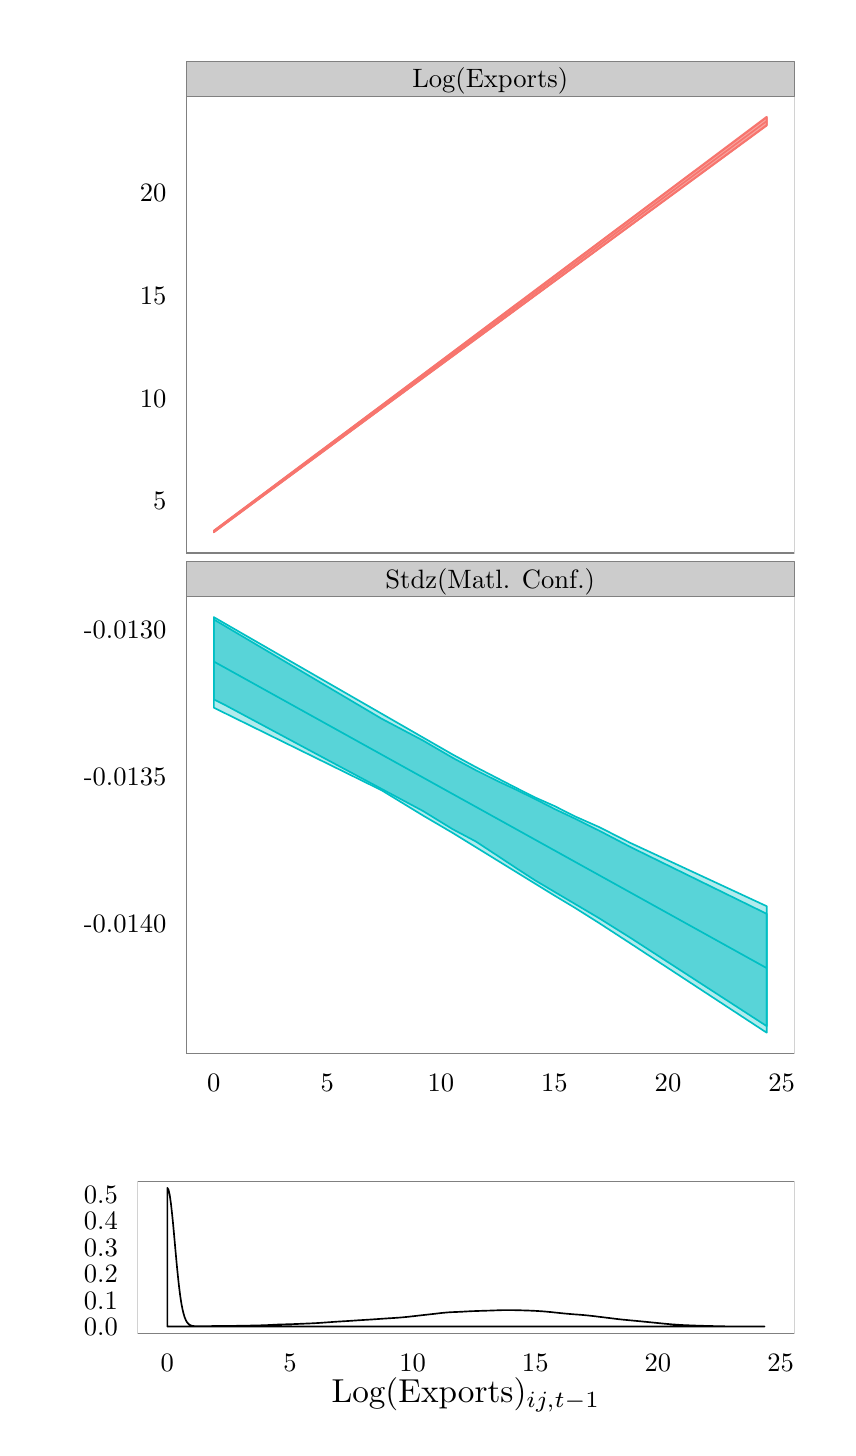
\begin{tikzpicture}[x=1pt,y=1pt]
\definecolor[named]{fillColor}{rgb}{1.00,1.00,1.00}
\path[use as bounding box,fill=fillColor,fill opacity=0.00] (0,0) rectangle (289.08,505.89);
\begin{scope}
\path[clip] (  0.00,101.18) rectangle (289.08,505.89);
\definecolor[named]{drawColor}{rgb}{1.00,1.00,1.00}
\definecolor[named]{fillColor}{rgb}{1.00,1.00,1.00}

\path[draw=drawColor,line width= 0.6pt,line join=round,line cap=round,fill=fillColor] ( -0.00,101.18) rectangle (289.08,505.89);
\end{scope}
\begin{scope}
\path[clip] ( 57.28,316.03) rectangle (277.04,481.21);
\definecolor[named]{fillColor}{rgb}{1.00,1.00,1.00}

\path[fill=fillColor] ( 57.28,316.03) rectangle (277.03,481.21);
\definecolor[named]{drawColor}{rgb}{0.97,0.46,0.43}

\path[draw=drawColor,line width= 0.6pt,line join=round] ( 67.27,323.86) --
	( 71.57,327.06) --
	(127.91,368.87) --
	(142.85,379.95) --
	(153.63,387.95) --
	(161.92,394.10) --
	(169.48,399.71) --
	(176.53,404.95) --
	(183.32,409.99) --
	(190.38,415.22) --
	(197.85,420.77) --
	(206.59,427.25) --
	(217.83,435.60) --
	(267.05,472.12);
\definecolor[named]{fillColor}{rgb}{0.97,0.46,0.43}

\path[draw=drawColor,line width= 0.6pt,line join=round,line cap=round,fill=fillColor,fill opacity=0.30] ( 67.27,324.13) --
	( 71.57,327.34) --
	(127.91,369.47) --
	(142.85,380.67) --
	(153.63,388.75) --
	(161.92,394.97) --
	(169.48,400.64) --
	(176.53,405.92) --
	(183.32,411.00) --
	(190.38,416.28) --
	(197.85,421.87) --
	(206.59,428.41) --
	(217.83,436.82) --
	(267.05,473.70) --
	(267.05,470.51) --
	(217.83,434.38) --
	(206.59,426.12) --
	(197.85,419.71) --
	(190.38,414.21) --
	(183.32,409.03) --
	(176.53,404.03) --
	(169.48,398.85) --
	(161.92,393.30) --
	(153.63,387.20) --
	(142.85,379.29) --
	(127.91,368.30) --
	( 71.57,326.74) --
	( 67.27,323.54) --
	cycle;
\definecolor[named]{fillColor}{rgb}{0.97,0.46,0.43}

\path[draw=drawColor,line width= 0.6pt,line join=round,line cap=round,fill=fillColor,fill opacity=0.50] ( 67.27,324.08) --
	( 71.57,327.29) --
	(127.91,369.36) --
	(142.85,380.54) --
	(153.63,388.58) --
	(161.92,394.80) --
	(169.48,400.45) --
	(176.53,405.72) --
	(183.32,410.79) --
	(190.38,416.06) --
	(197.85,421.65) --
	(206.59,428.18) --
	(217.83,436.60) --
	(267.05,473.48) --
	(267.05,470.71) --
	(217.83,434.51) --
	(206.59,426.24) --
	(197.85,419.83) --
	(190.38,414.33) --
	(183.32,409.15) --
	(176.53,404.15) --
	(169.48,398.97) --
	(161.92,393.41) --
	(153.63,387.29) --
	(142.85,379.36) --
	(127.91,368.37) --
	( 71.57,326.77) --
	( 67.27,323.58) --
	cycle;
\definecolor[named]{drawColor}{rgb}{0.50,0.50,0.50}

\path[draw=drawColor,line width= 0.6pt,line join=round,line cap=round] ( 57.28,316.03) rectangle (277.03,481.21);
\end{scope}
\begin{scope}
\path[clip] ( 57.28,135.21) rectangle (277.04,300.39);
\definecolor[named]{fillColor}{rgb}{1.00,1.00,1.00}

\path[fill=fillColor] ( 57.28,135.21) rectangle (277.03,300.39);
\definecolor[named]{drawColor}{rgb}{0.00,0.75,0.77}

\path[draw=drawColor,line width= 0.6pt,line join=round] ( 67.27,276.84) --
	( 71.57,274.46) --
	(127.91,243.21) --
	(142.85,234.93) --
	(153.63,228.95) --
	(161.92,224.36) --
	(169.48,220.17) --
	(176.53,216.26) --
	(183.32,212.49) --
	(190.38,208.58) --
	(197.85,204.43) --
	(206.59,199.59) --
	(217.83,193.36) --
	(267.05,166.06);
\definecolor[named]{fillColor}{rgb}{0.00,0.75,0.77}

\path[draw=drawColor,line width= 0.6pt,line join=round,line cap=round,fill=fillColor,fill opacity=0.30] ( 67.27,292.88) --
	( 71.57,290.40) --
	(127.91,257.99) --
	(142.85,249.40) --
	(153.63,243.21) --
	(161.92,238.72) --
	(169.48,234.81) --
	(176.53,231.18) --
	(183.32,227.75) --
	(190.38,224.62) --
	(197.85,220.85) --
	(206.59,216.99) --
	(217.83,211.28) --
	(267.05,188.43) --
	(267.05,142.72) --
	(217.83,174.97) --
	(206.59,182.28) --
	(197.85,187.78) --
	(190.38,192.26) --
	(183.32,196.60) --
	(176.53,200.78) --
	(169.48,205.12) --
	(161.92,209.78) --
	(153.63,214.88) --
	(142.85,221.20) --
	(127.91,230.31) --
	( 71.57,258.04) --
	( 67.27,260.15) --
	cycle;
\definecolor[named]{fillColor}{rgb}{0.00,0.75,0.77}

\path[draw=drawColor,line width= 0.6pt,line join=round,line cap=round,fill=fillColor,fill opacity=0.50] ( 67.27,292.04) --
	( 71.57,289.50) --
	(127.91,256.18) --
	(142.85,248.30) --
	(153.63,242.02) --
	(161.92,237.57) --
	(169.48,233.80) --
	(176.53,230.50) --
	(183.32,227.18) --
	(190.38,223.56) --
	(197.85,220.03) --
	(206.59,215.69) --
	(217.83,209.81) --
	(267.05,185.68) --
	(267.05,145.09) --
	(217.83,176.99) --
	(206.59,184.03) --
	(197.85,189.20) --
	(190.38,193.61) --
	(183.32,197.80) --
	(176.53,202.20) --
	(169.48,206.86) --
	(161.92,211.83) --
	(153.63,216.22) --
	(142.85,222.83) --
	(127.91,230.81) --
	( 71.57,260.99) --
	( 67.27,263.13) --
	cycle;
\definecolor[named]{drawColor}{rgb}{0.50,0.50,0.50}

\path[draw=drawColor,line width= 0.6pt,line join=round,line cap=round] ( 57.28,135.21) rectangle (277.03,300.39);
\end{scope}
\begin{scope}
\path[clip] (  0.00,  0.00) rectangle (289.08,505.89);
\definecolor[named]{drawColor}{rgb}{0.50,0.50,0.50}
\definecolor[named]{fillColor}{rgb}{0.80,0.80,0.80}

\path[draw=drawColor,line width= 0.2pt,line join=round,line cap=round,fill=fillColor] ( 57.28,481.21) rectangle (277.03,493.84);
\definecolor[named]{drawColor}{rgb}{0.00,0.00,0.00}

\node[text=drawColor,anchor=base,inner sep=0pt, outer sep=0pt, scale=  0.96] at (167.16,484.22) {Log(Exports)};
\end{scope}
\begin{scope}
\path[clip] (  0.00,  0.00) rectangle (289.08,505.89);
\definecolor[named]{drawColor}{rgb}{0.50,0.50,0.50}
\definecolor[named]{fillColor}{rgb}{0.80,0.80,0.80}

\path[draw=drawColor,line width= 0.2pt,line join=round,line cap=round,fill=fillColor] ( 57.28,300.39) rectangle (277.03,313.02);
\definecolor[named]{drawColor}{rgb}{0.00,0.00,0.00}

\node[text=drawColor,anchor=base,inner sep=0pt, outer sep=0pt, scale=  0.96] at (167.16,303.40) {Stdz(Matl. Conf.)};
\end{scope}
\begin{scope}
\path[clip] (  0.00,  0.00) rectangle (289.08,505.89);
\definecolor[named]{drawColor}{rgb}{0.00,0.00,0.00}

\node[text=drawColor,anchor=base east,inner sep=0pt, outer sep=0pt, scale=  0.96] at ( 50.17,331.61) {5};

\node[text=drawColor,anchor=base east,inner sep=0pt, outer sep=0pt, scale=  0.96] at ( 50.17,368.71) {10};

\node[text=drawColor,anchor=base east,inner sep=0pt, outer sep=0pt, scale=  0.96] at ( 50.17,405.80) {15};

\node[text=drawColor,anchor=base east,inner sep=0pt, outer sep=0pt, scale=  0.96] at ( 50.17,442.90) {20};
\end{scope}
\begin{scope}
\path[clip] (  0.00,  0.00) rectangle (289.08,505.89);
\definecolor[named]{drawColor}{rgb}{0.00,0.00,0.00}

\node[text=drawColor,anchor=base east,inner sep=0pt, outer sep=0pt, scale=  0.96] at ( 50.17,178.96) {-0.0140};

\node[text=drawColor,anchor=base east,inner sep=0pt, outer sep=0pt, scale=  0.96] at ( 50.17,232.03) {-0.0135};

\node[text=drawColor,anchor=base east,inner sep=0pt, outer sep=0pt, scale=  0.96] at ( 50.17,285.10) {-0.0130};
\end{scope}
\begin{scope}
\path[clip] (  0.00,  0.00) rectangle (289.08,505.89);
\definecolor[named]{drawColor}{rgb}{0.00,0.00,0.00}

\node[text=drawColor,anchor=base,inner sep=0pt, outer sep=0pt, scale=  0.96] at ( 67.27,121.49) {0};

\node[text=drawColor,anchor=base,inner sep=0pt, outer sep=0pt, scale=  0.96] at (108.30,121.49) {5};

\node[text=drawColor,anchor=base,inner sep=0pt, outer sep=0pt, scale=  0.96] at (149.33,121.49) {10};

\node[text=drawColor,anchor=base,inner sep=0pt, outer sep=0pt, scale=  0.96] at (190.36,121.49) {15};

\node[text=drawColor,anchor=base,inner sep=0pt, outer sep=0pt, scale=  0.96] at (231.39,121.49) {20};

\node[text=drawColor,anchor=base,inner sep=0pt, outer sep=0pt, scale=  0.96] at (272.42,121.49) {25};
\end{scope}
\begin{scope}
\path[clip] (  0.00,  0.00) rectangle (289.08,101.18);
\definecolor[named]{drawColor}{rgb}{1.00,1.00,1.00}
\definecolor[named]{fillColor}{rgb}{1.00,1.00,1.00}

\path[draw=drawColor,line width= 0.6pt,line join=round,line cap=round,fill=fillColor] (  0.00,  0.00) rectangle (289.08,101.18);
\end{scope}
\begin{scope}
\path[clip] ( 39.69, 34.03) rectangle (277.03, 89.13);
\definecolor[named]{fillColor}{rgb}{1.00,1.00,1.00}

\path[fill=fillColor] ( 39.69, 34.03) rectangle (277.03, 89.13);
\definecolor[named]{drawColor}{rgb}{0.00,0.00,0.00}

\path[draw=drawColor,line width= 0.6pt,line join=round,line cap=round] ( 50.48, 86.63) --
	( 50.90, 85.95) --
	( 51.32, 84.10) --
	( 51.74, 81.21) --
	( 52.16, 77.49) --
	( 52.59, 73.16) --
	( 53.01, 68.50) --
	( 53.43, 63.75) --
	( 53.85, 59.13) --
	( 54.28, 54.82) --
	( 54.70, 50.97) --
	( 55.12, 47.63) --
	( 55.54, 44.91) --
	( 55.96, 42.71) --
	( 56.39, 40.98) --
	( 56.81, 39.67) --
	( 57.23, 38.70) --
	( 57.65, 38.00) --
	( 58.08, 37.52) --
	( 58.50, 37.19) --
	( 58.92, 36.97) --
	( 59.34, 36.83) --
	( 59.76, 36.75) --
	( 60.19, 36.70) --
	( 60.61, 36.68) --
	( 61.03, 36.66) --
	( 61.45, 36.65) --
	( 61.88, 36.65) --
	( 62.30, 36.65) --
	( 62.72, 36.65) --
	( 63.14, 36.66) --
	( 63.56, 36.66) --
	( 63.99, 36.67) --
	( 64.41, 36.67) --
	( 64.83, 36.68) --
	( 65.25, 36.69) --
	( 65.68, 36.69) --
	( 66.10, 36.70) --
	( 66.52, 36.71) --
	( 66.94, 36.71) --
	( 67.37, 36.72) --
	( 67.79, 36.73) --
	( 68.21, 36.73) --
	( 68.63, 36.74) --
	( 69.05, 36.74) --
	( 69.48, 36.75) --
	( 69.90, 36.75) --
	( 70.32, 36.76) --
	( 70.74, 36.76) --
	( 71.17, 36.76) --
	( 71.59, 36.77) --
	( 72.01, 36.77) --
	( 72.43, 36.78) --
	( 72.85, 36.78) --
	( 73.28, 36.78) --
	( 73.70, 36.79) --
	( 74.12, 36.79) --
	( 74.54, 36.79) --
	( 74.97, 36.80) --
	( 75.39, 36.80) --
	( 75.81, 36.81) --
	( 76.23, 36.81) --
	( 76.65, 36.82) --
	( 77.08, 36.83) --
	( 77.50, 36.83) --
	( 77.92, 36.84) --
	( 78.34, 36.85) --
	( 78.77, 36.86) --
	( 79.19, 36.86) --
	( 79.61, 36.87) --
	( 80.03, 36.88) --
	( 80.46, 36.89) --
	( 80.88, 36.90) --
	( 81.30, 36.91) --
	( 81.72, 36.92) --
	( 82.14, 36.93) --
	( 82.57, 36.94) --
	( 82.99, 36.95) --
	( 83.41, 36.96) --
	( 83.83, 36.97) --
	( 84.26, 36.98) --
	( 84.68, 36.99) --
	( 85.10, 37.01) --
	( 85.52, 37.02) --
	( 85.94, 37.04) --
	( 86.37, 37.05) --
	( 86.79, 37.07) --
	( 87.21, 37.10) --
	( 87.63, 37.12) --
	( 88.06, 37.14) --
	( 88.48, 37.16) --
	( 88.90, 37.19) --
	( 89.32, 37.21) --
	( 89.74, 37.23) --
	( 90.17, 37.25) --
	( 90.59, 37.27) --
	( 91.01, 37.28) --
	( 91.43, 37.30) --
	( 91.86, 37.31) --
	( 92.28, 37.32) --
	( 92.70, 37.33) --
	( 93.12, 37.34) --
	( 93.54, 37.35) --
	( 93.97, 37.36) --
	( 94.39, 37.37) --
	( 94.81, 37.38) --
	( 95.23, 37.39) --
	( 95.66, 37.41) --
	( 96.08, 37.43) --
	( 96.50, 37.44) --
	( 96.92, 37.46) --
	( 97.35, 37.48) --
	( 97.77, 37.49) --
	( 98.19, 37.51) --
	( 98.61, 37.53) --
	( 99.03, 37.55) --
	( 99.46, 37.56) --
	( 99.88, 37.58) --
	(100.30, 37.60) --
	(100.72, 37.62) --
	(101.15, 37.63) --
	(101.57, 37.65) --
	(101.99, 37.67) --
	(102.41, 37.69) --
	(102.83, 37.71) --
	(103.26, 37.73) --
	(103.68, 37.75) --
	(104.10, 37.78) --
	(104.52, 37.80) --
	(104.95, 37.82) --
	(105.37, 37.85) --
	(105.79, 37.88) --
	(106.21, 37.91) --
	(106.63, 37.94) --
	(107.06, 37.97) --
	(107.48, 38.00) --
	(107.90, 38.03) --
	(108.32, 38.06) --
	(108.75, 38.09) --
	(109.17, 38.12) --
	(109.59, 38.15) --
	(110.01, 38.19) --
	(110.44, 38.22) --
	(110.86, 38.24) --
	(111.28, 38.27) --
	(111.70, 38.30) --
	(112.12, 38.33) --
	(112.55, 38.35) --
	(112.97, 38.38) --
	(113.39, 38.40) --
	(113.81, 38.43) --
	(114.24, 38.45) --
	(114.66, 38.48) --
	(115.08, 38.51) --
	(115.50, 38.53) --
	(115.92, 38.56) --
	(116.35, 38.59) --
	(116.77, 38.62) --
	(117.19, 38.64) --
	(117.61, 38.67) --
	(118.04, 38.70) --
	(118.46, 38.73) --
	(118.88, 38.76) --
	(119.30, 38.79) --
	(119.72, 38.82) --
	(120.15, 38.84) --
	(120.57, 38.87) --
	(120.99, 38.89) --
	(121.41, 38.92) --
	(121.84, 38.95) --
	(122.26, 38.97) --
	(122.68, 39.00) --
	(123.10, 39.02) --
	(123.52, 39.05) --
	(123.95, 39.07) --
	(124.37, 39.10) --
	(124.79, 39.13) --
	(125.21, 39.16) --
	(125.64, 39.19) --
	(126.06, 39.22) --
	(126.48, 39.25) --
	(126.90, 39.28) --
	(127.33, 39.31) --
	(127.75, 39.34) --
	(128.17, 39.37) --
	(128.59, 39.40) --
	(129.01, 39.42) --
	(129.44, 39.45) --
	(129.86, 39.48) --
	(130.28, 39.51) --
	(130.70, 39.53) --
	(131.13, 39.56) --
	(131.55, 39.59) --
	(131.97, 39.61) --
	(132.39, 39.64) --
	(132.81, 39.67) --
	(133.24, 39.70) --
	(133.66, 39.73) --
	(134.08, 39.76) --
	(134.50, 39.79) --
	(134.93, 39.83) --
	(135.35, 39.86) --
	(135.77, 39.90) --
	(136.19, 39.94) --
	(136.61, 39.98) --
	(137.04, 40.02) --
	(137.46, 40.07) --
	(137.88, 40.11) --
	(138.30, 40.16) --
	(138.73, 40.21) --
	(139.15, 40.25) --
	(139.57, 40.30) --
	(139.99, 40.35) --
	(140.42, 40.40) --
	(140.84, 40.45) --
	(141.26, 40.50) --
	(141.68, 40.54) --
	(142.10, 40.59) --
	(142.53, 40.64) --
	(142.95, 40.69) --
	(143.37, 40.74) --
	(143.79, 40.78) --
	(144.22, 40.83) --
	(144.64, 40.88) --
	(145.06, 40.92) --
	(145.48, 40.97) --
	(145.90, 41.02) --
	(146.33, 41.07) --
	(146.75, 41.11) --
	(147.17, 41.16) --
	(147.59, 41.21) --
	(148.02, 41.26) --
	(148.44, 41.31) --
	(148.86, 41.36) --
	(149.28, 41.41) --
	(149.70, 41.46) --
	(150.13, 41.50) --
	(150.55, 41.54) --
	(150.97, 41.58) --
	(151.39, 41.62) --
	(151.82, 41.65) --
	(152.24, 41.68) --
	(152.66, 41.71) --
	(153.08, 41.73) --
	(153.50, 41.75) --
	(153.93, 41.77) --
	(154.35, 41.79) --
	(154.77, 41.80) --
	(155.19, 41.82) --
	(155.62, 41.84) --
	(156.04, 41.86) --
	(156.46, 41.88) --
	(156.88, 41.90) --
	(157.31, 41.92) --
	(157.73, 41.95) --
	(158.15, 41.97) --
	(158.57, 41.99) --
	(158.99, 42.02) --
	(159.42, 42.04) --
	(159.84, 42.06) --
	(160.26, 42.08) --
	(160.68, 42.10) --
	(161.11, 42.12) --
	(161.53, 42.13) --
	(161.95, 42.15) --
	(162.37, 42.16) --
	(162.79, 42.18) --
	(163.22, 42.19) --
	(163.64, 42.21) --
	(164.06, 42.22) --
	(164.48, 42.23) --
	(164.91, 42.25) --
	(165.33, 42.26) --
	(165.75, 42.27) --
	(166.17, 42.29) --
	(166.59, 42.30) --
	(167.02, 42.31) --
	(167.44, 42.33) --
	(167.86, 42.34) --
	(168.28, 42.36) --
	(168.71, 42.37) --
	(169.13, 42.39) --
	(169.55, 42.40) --
	(169.97, 42.42) --
	(170.39, 42.43) --
	(170.82, 42.44) --
	(171.24, 42.46) --
	(171.66, 42.47) --
	(172.08, 42.48) --
	(172.51, 42.48) --
	(172.93, 42.49) --
	(173.35, 42.49) --
	(173.77, 42.49) --
	(174.20, 42.49) --
	(174.62, 42.49) --
	(175.04, 42.48) --
	(175.46, 42.47) --
	(175.88, 42.46) --
	(176.31, 42.45) --
	(176.73, 42.44) --
	(177.15, 42.43) --
	(177.57, 42.42) --
	(178.00, 42.41) --
	(178.42, 42.40) --
	(178.84, 42.39) --
	(179.26, 42.37) --
	(179.68, 42.36) --
	(180.11, 42.35) --
	(180.53, 42.33) --
	(180.95, 42.32) --
	(181.37, 42.30) --
	(181.80, 42.28) --
	(182.22, 42.27) --
	(182.64, 42.25) --
	(183.06, 42.23) --
	(183.48, 42.20) --
	(183.91, 42.18) --
	(184.33, 42.16) --
	(184.75, 42.13) --
	(185.17, 42.10) --
	(185.60, 42.07) --
	(186.02, 42.04) --
	(186.44, 42.01) --
	(186.86, 41.98) --
	(187.29, 41.94) --
	(187.71, 41.90) --
	(188.13, 41.86) --
	(188.55, 41.82) --
	(188.97, 41.78) --
	(189.40, 41.74) --
	(189.82, 41.69) --
	(190.24, 41.65) --
	(190.66, 41.60) --
	(191.09, 41.56) --
	(191.51, 41.51) --
	(191.93, 41.47) --
	(192.35, 41.42) --
	(192.77, 41.38) --
	(193.20, 41.34) --
	(193.62, 41.29) --
	(194.04, 41.25) --
	(194.46, 41.21) --
	(194.89, 41.17) --
	(195.31, 41.14) --
	(195.73, 41.10) --
	(196.15, 41.06) --
	(196.57, 41.03) --
	(197.00, 41.00) --
	(197.42, 40.96) --
	(197.84, 40.93) --
	(198.26, 40.90) --
	(198.69, 40.87) --
	(199.11, 40.84) --
	(199.53, 40.80) --
	(199.95, 40.77) --
	(200.37, 40.73) --
	(200.80, 40.70) --
	(201.22, 40.66) --
	(201.64, 40.62) --
	(202.06, 40.58) --
	(202.49, 40.54) --
	(202.91, 40.49) --
	(203.33, 40.44) --
	(203.75, 40.40) --
	(204.18, 40.35) --
	(204.60, 40.30) --
	(205.02, 40.25) --
	(205.44, 40.20) --
	(205.86, 40.14) --
	(206.29, 40.09) --
	(206.71, 40.04) --
	(207.13, 39.99) --
	(207.55, 39.94) --
	(207.98, 39.89) --
	(208.40, 39.84) --
	(208.82, 39.78) --
	(209.24, 39.73) --
	(209.66, 39.68) --
	(210.09, 39.63) --
	(210.51, 39.58) --
	(210.93, 39.52) --
	(211.35, 39.47) --
	(211.78, 39.42) --
	(212.20, 39.36) --
	(212.62, 39.31) --
	(213.04, 39.26) --
	(213.46, 39.21) --
	(213.89, 39.17) --
	(214.31, 39.12) --
	(214.73, 39.07) --
	(215.15, 39.03) --
	(215.58, 38.99) --
	(216.00, 38.95) --
	(216.42, 38.91) --
	(216.84, 38.87) --
	(217.27, 38.83) --
	(217.69, 38.79) --
	(218.11, 38.75) --
	(218.53, 38.71) --
	(218.95, 38.67) --
	(219.38, 38.63) --
	(219.80, 38.59) --
	(220.22, 38.55) --
	(220.64, 38.51) --
	(221.07, 38.47) --
	(221.49, 38.43) --
	(221.91, 38.39) --
	(222.33, 38.35) --
	(222.75, 38.30) --
	(223.18, 38.26) --
	(223.60, 38.22) --
	(224.02, 38.18) --
	(224.44, 38.14) --
	(224.87, 38.09) --
	(225.29, 38.05) --
	(225.71, 38.01) --
	(226.13, 37.97) --
	(226.55, 37.93) --
	(226.98, 37.88) --
	(227.40, 37.84) --
	(227.82, 37.80) --
	(228.24, 37.76) --
	(228.67, 37.72) --
	(229.09, 37.67) --
	(229.51, 37.63) --
	(229.93, 37.59) --
	(230.35, 37.55) --
	(230.78, 37.51) --
	(231.20, 37.47) --
	(231.62, 37.44) --
	(232.04, 37.40) --
	(232.47, 37.36) --
	(232.89, 37.33) --
	(233.31, 37.30) --
	(233.73, 37.27) --
	(234.16, 37.24) --
	(234.58, 37.21) --
	(235.00, 37.18) --
	(235.42, 37.15) --
	(235.84, 37.13) --
	(236.27, 37.11) --
	(236.69, 37.08) --
	(237.11, 37.06) --
	(237.53, 37.04) --
	(237.96, 37.02) --
	(238.38, 37.00) --
	(238.80, 36.99) --
	(239.22, 36.97) --
	(239.64, 36.95) --
	(240.07, 36.94) --
	(240.49, 36.92) --
	(240.91, 36.91) --
	(241.33, 36.89) --
	(241.76, 36.88) --
	(242.18, 36.87) --
	(242.60, 36.85) --
	(243.02, 36.84) --
	(243.44, 36.83) --
	(243.87, 36.81) --
	(244.29, 36.80) --
	(244.71, 36.79) --
	(245.13, 36.78) --
	(245.56, 36.77) --
	(245.98, 36.76) --
	(246.40, 36.75) --
	(246.82, 36.74) --
	(247.25, 36.73) --
	(247.67, 36.71) --
	(248.09, 36.70) --
	(248.51, 36.69) --
	(248.93, 36.68) --
	(249.36, 36.67) --
	(249.78, 36.66) --
	(250.20, 36.65) --
	(250.62, 36.64) --
	(251.05, 36.64) --
	(251.47, 36.63) --
	(251.89, 36.62) --
	(252.31, 36.61) --
	(252.73, 36.61) --
	(253.16, 36.60) --
	(253.58, 36.60) --
	(254.00, 36.59) --
	(254.42, 36.59) --
	(254.85, 36.59) --
	(255.27, 36.58) --
	(255.69, 36.58) --
	(256.11, 36.58) --
	(256.53, 36.57) --
	(256.96, 36.57) --
	(257.38, 36.57) --
	(257.80, 36.57) --
	(258.22, 36.57) --
	(258.65, 36.56) --
	(259.07, 36.56) --
	(259.49, 36.56) --
	(259.91, 36.56) --
	(260.33, 36.56) --
	(260.76, 36.56) --
	(261.18, 36.56) --
	(261.60, 36.56) --
	(262.02, 36.55) --
	(262.45, 36.55) --
	(262.87, 36.55) --
	(263.29, 36.55) --
	(263.71, 36.55) --
	(264.14, 36.55) --
	(264.56, 36.55) --
	(264.98, 36.55) --
	(265.40, 36.55) --
	(265.82, 36.55) --
	(266.25, 36.54) --
	(266.25, 36.54) --
	(265.82, 36.54) --
	(265.40, 36.54) --
	(264.98, 36.54) --
	(264.56, 36.54) --
	(264.14, 36.54) --
	(263.71, 36.54) --
	(263.29, 36.54) --
	(262.87, 36.54) --
	(262.45, 36.54) --
	(262.02, 36.54) --
	(261.60, 36.54) --
	(261.18, 36.54) --
	(260.76, 36.54) --
	(260.33, 36.54) --
	(259.91, 36.54) --
	(259.49, 36.54) --
	(259.07, 36.54) --
	(258.65, 36.54) --
	(258.22, 36.54) --
	(257.80, 36.54) --
	(257.38, 36.54) --
	(256.96, 36.54) --
	(256.53, 36.54) --
	(256.11, 36.54) --
	(255.69, 36.54) --
	(255.27, 36.54) --
	(254.85, 36.54) --
	(254.42, 36.54) --
	(254.00, 36.54) --
	(253.58, 36.54) --
	(253.16, 36.54) --
	(252.73, 36.54) --
	(252.31, 36.54) --
	(251.89, 36.54) --
	(251.47, 36.54) --
	(251.05, 36.54) --
	(250.62, 36.54) --
	(250.20, 36.54) --
	(249.78, 36.54) --
	(249.36, 36.54) --
	(248.93, 36.54) --
	(248.51, 36.54) --
	(248.09, 36.54) --
	(247.67, 36.54) --
	(247.25, 36.54) --
	(246.82, 36.54) --
	(246.40, 36.54) --
	(245.98, 36.54) --
	(245.56, 36.54) --
	(245.13, 36.54) --
	(244.71, 36.54) --
	(244.29, 36.54) --
	(243.87, 36.54) --
	(243.44, 36.54) --
	(243.02, 36.54) --
	(242.60, 36.54) --
	(242.18, 36.54) --
	(241.76, 36.54) --
	(241.33, 36.54) --
	(240.91, 36.54) --
	(240.49, 36.54) --
	(240.07, 36.54) --
	(239.64, 36.54) --
	(239.22, 36.54) --
	(238.80, 36.54) --
	(238.38, 36.54) --
	(237.96, 36.54) --
	(237.53, 36.54) --
	(237.11, 36.54) --
	(236.69, 36.54) --
	(236.27, 36.54) --
	(235.84, 36.54) --
	(235.42, 36.54) --
	(235.00, 36.54) --
	(234.58, 36.54) --
	(234.16, 36.54) --
	(233.73, 36.54) --
	(233.31, 36.54) --
	(232.89, 36.54) --
	(232.47, 36.54) --
	(232.04, 36.54) --
	(231.62, 36.54) --
	(231.20, 36.54) --
	(230.78, 36.54) --
	(230.35, 36.54) --
	(229.93, 36.54) --
	(229.51, 36.54) --
	(229.09, 36.54) --
	(228.67, 36.54) --
	(228.24, 36.54) --
	(227.82, 36.54) --
	(227.40, 36.54) --
	(226.98, 36.54) --
	(226.55, 36.54) --
	(226.13, 36.54) --
	(225.71, 36.54) --
	(225.29, 36.54) --
	(224.87, 36.54) --
	(224.44, 36.54) --
	(224.02, 36.54) --
	(223.60, 36.54) --
	(223.18, 36.54) --
	(222.75, 36.54) --
	(222.33, 36.54) --
	(221.91, 36.54) --
	(221.49, 36.54) --
	(221.07, 36.54) --
	(220.64, 36.54) --
	(220.22, 36.54) --
	(219.80, 36.54) --
	(219.38, 36.54) --
	(218.95, 36.54) --
	(218.53, 36.54) --
	(218.11, 36.54) --
	(217.69, 36.54) --
	(217.27, 36.54) --
	(216.84, 36.54) --
	(216.42, 36.54) --
	(216.00, 36.54) --
	(215.58, 36.54) --
	(215.15, 36.54) --
	(214.73, 36.54) --
	(214.31, 36.54) --
	(213.89, 36.54) --
	(213.46, 36.54) --
	(213.04, 36.54) --
	(212.62, 36.54) --
	(212.20, 36.54) --
	(211.78, 36.54) --
	(211.35, 36.54) --
	(210.93, 36.54) --
	(210.51, 36.54) --
	(210.09, 36.54) --
	(209.66, 36.54) --
	(209.24, 36.54) --
	(208.82, 36.54) --
	(208.40, 36.54) --
	(207.98, 36.54) --
	(207.55, 36.54) --
	(207.13, 36.54) --
	(206.71, 36.54) --
	(206.29, 36.54) --
	(205.86, 36.54) --
	(205.44, 36.54) --
	(205.02, 36.54) --
	(204.60, 36.54) --
	(204.18, 36.54) --
	(203.75, 36.54) --
	(203.33, 36.54) --
	(202.91, 36.54) --
	(202.49, 36.54) --
	(202.06, 36.54) --
	(201.64, 36.54) --
	(201.22, 36.54) --
	(200.80, 36.54) --
	(200.37, 36.54) --
	(199.95, 36.54) --
	(199.53, 36.54) --
	(199.11, 36.54) --
	(198.69, 36.54) --
	(198.26, 36.54) --
	(197.84, 36.54) --
	(197.42, 36.54) --
	(197.00, 36.54) --
	(196.57, 36.54) --
	(196.15, 36.54) --
	(195.73, 36.54) --
	(195.31, 36.54) --
	(194.89, 36.54) --
	(194.46, 36.54) --
	(194.04, 36.54) --
	(193.62, 36.54) --
	(193.20, 36.54) --
	(192.77, 36.54) --
	(192.35, 36.54) --
	(191.93, 36.54) --
	(191.51, 36.54) --
	(191.09, 36.54) --
	(190.66, 36.54) --
	(190.24, 36.54) --
	(189.82, 36.54) --
	(189.40, 36.54) --
	(188.97, 36.54) --
	(188.55, 36.54) --
	(188.13, 36.54) --
	(187.71, 36.54) --
	(187.29, 36.54) --
	(186.86, 36.54) --
	(186.44, 36.54) --
	(186.02, 36.54) --
	(185.60, 36.54) --
	(185.17, 36.54) --
	(184.75, 36.54) --
	(184.33, 36.54) --
	(183.91, 36.54) --
	(183.48, 36.54) --
	(183.06, 36.54) --
	(182.64, 36.54) --
	(182.22, 36.54) --
	(181.80, 36.54) --
	(181.37, 36.54) --
	(180.95, 36.54) --
	(180.53, 36.54) --
	(180.11, 36.54) --
	(179.68, 36.54) --
	(179.26, 36.54) --
	(178.84, 36.54) --
	(178.42, 36.54) --
	(178.00, 36.54) --
	(177.57, 36.54) --
	(177.15, 36.54) --
	(176.73, 36.54) --
	(176.31, 36.54) --
	(175.88, 36.54) --
	(175.46, 36.54) --
	(175.04, 36.54) --
	(174.62, 36.54) --
	(174.20, 36.54) --
	(173.77, 36.54) --
	(173.35, 36.54) --
	(172.93, 36.54) --
	(172.51, 36.54) --
	(172.08, 36.54) --
	(171.66, 36.54) --
	(171.24, 36.54) --
	(170.82, 36.54) --
	(170.39, 36.54) --
	(169.97, 36.54) --
	(169.55, 36.54) --
	(169.13, 36.54) --
	(168.71, 36.54) --
	(168.28, 36.54) --
	(167.86, 36.54) --
	(167.44, 36.54) --
	(167.02, 36.54) --
	(166.59, 36.54) --
	(166.17, 36.54) --
	(165.75, 36.54) --
	(165.33, 36.54) --
	(164.91, 36.54) --
	(164.48, 36.54) --
	(164.06, 36.54) --
	(163.64, 36.54) --
	(163.22, 36.54) --
	(162.79, 36.54) --
	(162.37, 36.54) --
	(161.95, 36.54) --
	(161.53, 36.54) --
	(161.11, 36.54) --
	(160.68, 36.54) --
	(160.26, 36.54) --
	(159.84, 36.54) --
	(159.42, 36.54) --
	(158.99, 36.54) --
	(158.57, 36.54) --
	(158.15, 36.54) --
	(157.73, 36.54) --
	(157.31, 36.54) --
	(156.88, 36.54) --
	(156.46, 36.54) --
	(156.04, 36.54) --
	(155.62, 36.54) --
	(155.19, 36.54) --
	(154.77, 36.54) --
	(154.35, 36.54) --
	(153.93, 36.54) --
	(153.50, 36.54) --
	(153.08, 36.54) --
	(152.66, 36.54) --
	(152.24, 36.54) --
	(151.82, 36.54) --
	(151.39, 36.54) --
	(150.97, 36.54) --
	(150.55, 36.54) --
	(150.13, 36.54) --
	(149.70, 36.54) --
	(149.28, 36.54) --
	(148.86, 36.54) --
	(148.44, 36.54) --
	(148.02, 36.54) --
	(147.59, 36.54) --
	(147.17, 36.54) --
	(146.75, 36.54) --
	(146.33, 36.54) --
	(145.90, 36.54) --
	(145.48, 36.54) --
	(145.06, 36.54) --
	(144.64, 36.54) --
	(144.22, 36.54) --
	(143.79, 36.54) --
	(143.37, 36.54) --
	(142.95, 36.54) --
	(142.53, 36.54) --
	(142.10, 36.54) --
	(141.68, 36.54) --
	(141.26, 36.54) --
	(140.84, 36.54) --
	(140.42, 36.54) --
	(139.99, 36.54) --
	(139.57, 36.54) --
	(139.15, 36.54) --
	(138.73, 36.54) --
	(138.30, 36.54) --
	(137.88, 36.54) --
	(137.46, 36.54) --
	(137.04, 36.54) --
	(136.61, 36.54) --
	(136.19, 36.54) --
	(135.77, 36.54) --
	(135.35, 36.54) --
	(134.93, 36.54) --
	(134.50, 36.54) --
	(134.08, 36.54) --
	(133.66, 36.54) --
	(133.24, 36.54) --
	(132.81, 36.54) --
	(132.39, 36.54) --
	(131.97, 36.54) --
	(131.55, 36.54) --
	(131.13, 36.54) --
	(130.70, 36.54) --
	(130.28, 36.54) --
	(129.86, 36.54) --
	(129.44, 36.54) --
	(129.01, 36.54) --
	(128.59, 36.54) --
	(128.17, 36.54) --
	(127.75, 36.54) --
	(127.33, 36.54) --
	(126.90, 36.54) --
	(126.48, 36.54) --
	(126.06, 36.54) --
	(125.64, 36.54) --
	(125.21, 36.54) --
	(124.79, 36.54) --
	(124.37, 36.54) --
	(123.95, 36.54) --
	(123.52, 36.54) --
	(123.10, 36.54) --
	(122.68, 36.54) --
	(122.26, 36.54) --
	(121.84, 36.54) --
	(121.41, 36.54) --
	(120.99, 36.54) --
	(120.57, 36.54) --
	(120.15, 36.54) --
	(119.72, 36.54) --
	(119.30, 36.54) --
	(118.88, 36.54) --
	(118.46, 36.54) --
	(118.04, 36.54) --
	(117.61, 36.54) --
	(117.19, 36.54) --
	(116.77, 36.54) --
	(116.35, 36.54) --
	(115.92, 36.54) --
	(115.50, 36.54) --
	(115.08, 36.54) --
	(114.66, 36.54) --
	(114.24, 36.54) --
	(113.81, 36.54) --
	(113.39, 36.54) --
	(112.97, 36.54) --
	(112.55, 36.54) --
	(112.12, 36.54) --
	(111.70, 36.54) --
	(111.28, 36.54) --
	(110.86, 36.54) --
	(110.44, 36.54) --
	(110.01, 36.54) --
	(109.59, 36.54) --
	(109.17, 36.54) --
	(108.75, 36.54) --
	(108.32, 36.54) --
	(107.90, 36.54) --
	(107.48, 36.54) --
	(107.06, 36.54) --
	(106.63, 36.54) --
	(106.21, 36.54) --
	(105.79, 36.54) --
	(105.37, 36.54) --
	(104.95, 36.54) --
	(104.52, 36.54) --
	(104.10, 36.54) --
	(103.68, 36.54) --
	(103.26, 36.54) --
	(102.83, 36.54) --
	(102.41, 36.54) --
	(101.99, 36.54) --
	(101.57, 36.54) --
	(101.15, 36.54) --
	(100.72, 36.54) --
	(100.30, 36.54) --
	( 99.88, 36.54) --
	( 99.46, 36.54) --
	( 99.03, 36.54) --
	( 98.61, 36.54) --
	( 98.19, 36.54) --
	( 97.77, 36.54) --
	( 97.35, 36.54) --
	( 96.92, 36.54) --
	( 96.50, 36.54) --
	( 96.08, 36.54) --
	( 95.66, 36.54) --
	( 95.23, 36.54) --
	( 94.81, 36.54) --
	( 94.39, 36.54) --
	( 93.97, 36.54) --
	( 93.54, 36.54) --
	( 93.12, 36.54) --
	( 92.70, 36.54) --
	( 92.28, 36.54) --
	( 91.86, 36.54) --
	( 91.43, 36.54) --
	( 91.01, 36.54) --
	( 90.59, 36.54) --
	( 90.17, 36.54) --
	( 89.74, 36.54) --
	( 89.32, 36.54) --
	( 88.90, 36.54) --
	( 88.48, 36.54) --
	( 88.06, 36.54) --
	( 87.63, 36.54) --
	( 87.21, 36.54) --
	( 86.79, 36.54) --
	( 86.37, 36.54) --
	( 85.94, 36.54) --
	( 85.52, 36.54) --
	( 85.10, 36.54) --
	( 84.68, 36.54) --
	( 84.26, 36.54) --
	( 83.83, 36.54) --
	( 83.41, 36.54) --
	( 82.99, 36.54) --
	( 82.57, 36.54) --
	( 82.14, 36.54) --
	( 81.72, 36.54) --
	( 81.30, 36.54) --
	( 80.88, 36.54) --
	( 80.46, 36.54) --
	( 80.03, 36.54) --
	( 79.61, 36.54) --
	( 79.19, 36.54) --
	( 78.77, 36.54) --
	( 78.34, 36.54) --
	( 77.92, 36.54) --
	( 77.50, 36.54) --
	( 77.08, 36.54) --
	( 76.65, 36.54) --
	( 76.23, 36.54) --
	( 75.81, 36.54) --
	( 75.39, 36.54) --
	( 74.97, 36.54) --
	( 74.54, 36.54) --
	( 74.12, 36.54) --
	( 73.70, 36.54) --
	( 73.28, 36.54) --
	( 72.85, 36.54) --
	( 72.43, 36.54) --
	( 72.01, 36.54) --
	( 71.59, 36.54) --
	( 71.17, 36.54) --
	( 70.74, 36.54) --
	( 70.32, 36.54) --
	( 69.90, 36.54) --
	( 69.48, 36.54) --
	( 69.05, 36.54) --
	( 68.63, 36.54) --
	( 68.21, 36.54) --
	( 67.79, 36.54) --
	( 67.37, 36.54) --
	( 66.94, 36.54) --
	( 66.52, 36.54) --
	( 66.10, 36.54) --
	( 65.68, 36.54) --
	( 65.25, 36.54) --
	( 64.83, 36.54) --
	( 64.41, 36.54) --
	( 63.99, 36.54) --
	( 63.56, 36.54) --
	( 63.14, 36.54) --
	( 62.72, 36.54) --
	( 62.30, 36.54) --
	( 61.88, 36.54) --
	( 61.45, 36.54) --
	( 61.03, 36.54) --
	( 60.61, 36.54) --
	( 60.19, 36.54) --
	( 59.76, 36.54) --
	( 59.34, 36.54) --
	( 58.92, 36.54) --
	( 58.50, 36.54) --
	( 58.08, 36.54) --
	( 57.65, 36.54) --
	( 57.23, 36.54) --
	( 56.81, 36.54) --
	( 56.39, 36.54) --
	( 55.96, 36.54) --
	( 55.54, 36.54) --
	( 55.12, 36.54) --
	( 54.70, 36.54) --
	( 54.28, 36.54) --
	( 53.85, 36.54) --
	( 53.43, 36.54) --
	( 53.01, 36.54) --
	( 52.59, 36.54) --
	( 52.16, 36.54) --
	( 51.74, 36.54) --
	( 51.32, 36.54) --
	( 50.90, 36.54) --
	( 50.48, 36.54) --
	( 50.48, 86.63);
\definecolor[named]{drawColor}{rgb}{0.50,0.50,0.50}

\path[draw=drawColor,line width= 0.6pt,line join=round,line cap=round] ( 39.69, 34.03) rectangle (277.03, 89.13);
\end{scope}
\begin{scope}
\path[clip] (  0.00,  0.00) rectangle (289.08,505.89);
\definecolor[named]{drawColor}{rgb}{0.00,0.00,0.00}

\node[text=drawColor,anchor=base east,inner sep=0pt, outer sep=0pt, scale=  0.96] at ( 32.57, 33.23) {0.0};

\node[text=drawColor,anchor=base east,inner sep=0pt, outer sep=0pt, scale=  0.96] at ( 32.57, 42.79) {0.1};

\node[text=drawColor,anchor=base east,inner sep=0pt, outer sep=0pt, scale=  0.96] at ( 32.57, 52.34) {0.2};

\node[text=drawColor,anchor=base east,inner sep=0pt, outer sep=0pt, scale=  0.96] at ( 32.57, 61.90) {0.3};

\node[text=drawColor,anchor=base east,inner sep=0pt, outer sep=0pt, scale=  0.96] at ( 32.57, 71.45) {0.4};

\node[text=drawColor,anchor=base east,inner sep=0pt, outer sep=0pt, scale=  0.96] at ( 32.57, 81.00) {0.5};
\end{scope}
\begin{scope}
\path[clip] (  0.00,  0.00) rectangle (289.08,505.89);
\definecolor[named]{drawColor}{rgb}{0.00,0.00,0.00}

\node[text=drawColor,anchor=base,inner sep=0pt, outer sep=0pt, scale=  0.96] at ( 50.48, 20.31) {0};

\node[text=drawColor,anchor=base,inner sep=0pt, outer sep=0pt, scale=  0.96] at ( 94.79, 20.31) {5};

\node[text=drawColor,anchor=base,inner sep=0pt, outer sep=0pt, scale=  0.96] at (139.10, 20.31) {10};

\node[text=drawColor,anchor=base,inner sep=0pt, outer sep=0pt, scale=  0.96] at (183.42, 20.31) {15};

\node[text=drawColor,anchor=base,inner sep=0pt, outer sep=0pt, scale=  0.96] at (227.73, 20.31) {20};

\node[text=drawColor,anchor=base,inner sep=0pt, outer sep=0pt, scale=  0.96] at (272.05, 20.31) {25};
\end{scope}
\begin{scope}
\path[clip] (  0.00,  0.00) rectangle (289.08,505.89);
\definecolor[named]{drawColor}{rgb}{0.00,0.00,0.00}

\node[text=drawColor,anchor=base,inner sep=0pt, outer sep=0pt, scale=  1.20] at (158.36,  9.03) {Log(Exports)$_{ij, t-1}$};
\end{scope}
\end{tikzpicture}
}  &
      \resizebox{.38\textwidth}{!}{% Created by tikzDevice version 0.7.0 on 2015-07-01 02:14:18
% !TEX encoding = UTF-8 Unicode
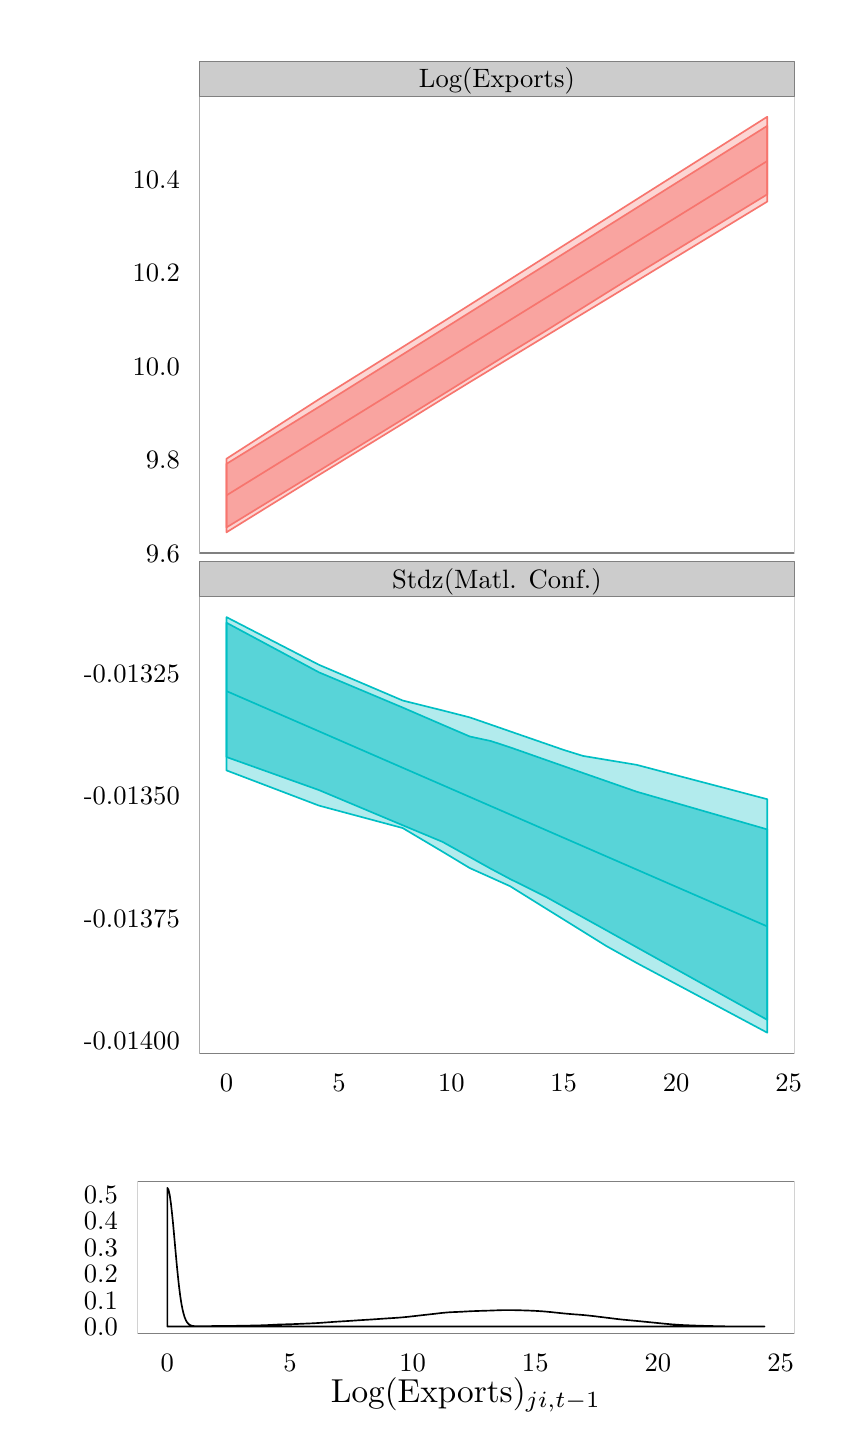
\begin{tikzpicture}[x=1pt,y=1pt]
\definecolor[named]{fillColor}{rgb}{1.00,1.00,1.00}
\path[use as bounding box,fill=fillColor,fill opacity=0.00] (0,0) rectangle (289.08,505.89);
\begin{scope}
\path[clip] (  0.00,101.18) rectangle (289.08,505.89);
\definecolor[named]{drawColor}{rgb}{1.00,1.00,1.00}
\definecolor[named]{fillColor}{rgb}{1.00,1.00,1.00}

\path[draw=drawColor,line width= 0.6pt,line join=round,line cap=round,fill=fillColor] (  0.00,101.18) rectangle (289.08,505.89);
\end{scope}
\begin{scope}
\path[clip] ( 62.08,316.03) rectangle (277.04,481.21);
\definecolor[named]{fillColor}{rgb}{1.00,1.00,1.00}

\path[fill=fillColor] ( 62.08,316.03) rectangle (277.03,481.21);
\definecolor[named]{drawColor}{rgb}{0.97,0.46,0.43}

\path[draw=drawColor,line width= 0.6pt,line join=round] ( 71.85,336.89) --
	(105.26,357.54) --
	(135.52,376.26) --
	(149.90,385.14) --
	(159.75,391.23) --
	(167.42,395.97) --
	(174.35,400.26) --
	(181.00,404.37) --
	(187.30,408.27) --
	(193.69,412.22) --
	(200.68,416.54) --
	(209.11,421.75) --
	(220.05,428.51) --
	(267.26,457.70);
\definecolor[named]{fillColor}{rgb}{0.97,0.46,0.43}

\path[draw=drawColor,line width= 0.6pt,line join=round,line cap=round,fill=fillColor,fill opacity=0.30] ( 71.85,350.12) --
	(105.26,371.61) --
	(135.52,390.49) --
	(149.90,399.50) --
	(159.75,405.72) --
	(167.42,410.57) --
	(174.35,414.95) --
	(181.00,419.16) --
	(187.30,423.14) --
	(193.69,427.18) --
	(200.68,431.60) --
	(209.11,436.93) --
	(220.05,443.85) --
	(267.26,473.70) --
	(267.26,443.05) --
	(220.05,414.35) --
	(209.11,407.71) --
	(200.68,402.61) --
	(193.69,398.37) --
	(187.30,394.49) --
	(181.00,390.67) --
	(174.35,386.64) --
	(167.42,382.44) --
	(159.75,377.79) --
	(149.90,371.74) --
	(135.52,362.82) --
	(105.26,344.24) --
	( 71.85,323.54) --
	cycle;
\definecolor[named]{fillColor}{rgb}{0.97,0.46,0.43}

\path[draw=drawColor,line width= 0.6pt,line join=round,line cap=round,fill=fillColor,fill opacity=0.50] ( 71.85,348.28) --
	(105.26,368.87) --
	(135.52,387.81) --
	(149.90,396.81) --
	(159.75,402.98) --
	(167.42,407.79) --
	(174.35,412.13) --
	(181.00,416.30) --
	(187.30,420.25) --
	(193.69,424.25) --
	(200.68,428.63) --
	(209.11,433.91) --
	(220.05,440.78) --
	(267.26,470.41) --
	(267.26,445.65) --
	(220.05,416.83) --
	(209.11,410.02) --
	(200.68,404.75) --
	(193.69,400.38) --
	(187.30,396.39) --
	(181.00,392.53) --
	(174.35,388.48) --
	(167.42,384.17) --
	(159.75,379.40) --
	(149.90,373.29) --
	(135.52,364.36) --
	(105.26,345.74) --
	( 71.85,325.30) --
	cycle;
\definecolor[named]{drawColor}{rgb}{0.50,0.50,0.50}

\path[draw=drawColor,line width= 0.6pt,line join=round,line cap=round] ( 62.08,316.03) rectangle (277.03,481.21);
\end{scope}
\begin{scope}
\path[clip] ( 62.08,135.21) rectangle (277.04,300.39);
\definecolor[named]{fillColor}{rgb}{1.00,1.00,1.00}

\path[fill=fillColor] ( 62.08,135.21) rectangle (277.03,300.39);
\definecolor[named]{drawColor}{rgb}{0.00,0.75,0.77}

\path[draw=drawColor,line width= 0.6pt,line join=round] ( 71.85,266.16) --
	(105.26,251.63) --
	(135.52,238.45) --
	(149.90,232.20) --
	(159.75,227.91) --
	(167.42,224.57) --
	(174.35,221.56) --
	(181.00,218.67) --
	(187.30,215.92) --
	(193.69,213.14) --
	(200.68,210.10) --
	(209.11,206.43) --
	(220.05,201.67) --
	(267.26,181.12);
\definecolor[named]{fillColor}{rgb}{0.00,0.75,0.77}

\path[draw=drawColor,line width= 0.6pt,line join=round,line cap=round,fill=fillColor,fill opacity=0.30] ( 71.85,292.88) --
	(105.26,275.66) --
	(135.52,262.75) --
	(149.90,259.18) --
	(159.75,256.66) --
	(167.42,254.01) --
	(174.35,251.60) --
	(181.00,249.30) --
	(187.30,247.12) --
	(193.69,244.90) --
	(200.68,242.73) --
	(209.11,241.33) --
	(220.05,239.51) --
	(267.26,227.09) --
	(267.26,142.72) --
	(220.05,167.93) --
	(209.11,174.03) --
	(200.68,179.28) --
	(193.69,183.62) --
	(187.30,187.58) --
	(181.00,191.50) --
	(174.35,195.64) --
	(167.42,198.77) --
	(159.75,202.21) --
	(149.90,208.14) --
	(135.52,216.67) --
	(105.26,224.78) --
	( 71.85,237.50) --
	cycle;
\definecolor[named]{fillColor}{rgb}{0.00,0.75,0.77}

\path[draw=drawColor,line width= 0.6pt,line join=round,line cap=round,fill=fillColor,fill opacity=0.50] ( 71.85,290.86) --
	(105.26,272.94) --
	(135.52,260.21) --
	(149.90,253.99) --
	(159.75,249.76) --
	(167.42,248.10) --
	(174.35,245.83) --
	(181.00,243.49) --
	(187.30,241.27) --
	(193.69,239.03) --
	(200.68,236.57) --
	(209.11,233.63) --
	(220.05,229.81) --
	(267.26,216.18) --
	(267.26,147.36) --
	(220.05,173.61) --
	(209.11,179.72) --
	(200.68,184.40) --
	(193.69,188.25) --
	(187.30,191.80) --
	(181.00,194.96) --
	(174.35,198.24) --
	(167.42,201.93) --
	(159.75,206.20) --
	(149.90,211.68) --
	(135.52,217.68) --
	(105.26,230.39) --
	( 71.85,242.33) --
	cycle;
\definecolor[named]{drawColor}{rgb}{0.50,0.50,0.50}

\path[draw=drawColor,line width= 0.6pt,line join=round,line cap=round] ( 62.08,135.21) rectangle (277.03,300.39);
\end{scope}
\begin{scope}
\path[clip] (  0.00,  0.00) rectangle (289.08,505.89);
\definecolor[named]{drawColor}{rgb}{0.50,0.50,0.50}
\definecolor[named]{fillColor}{rgb}{0.80,0.80,0.80}

\path[draw=drawColor,line width= 0.2pt,line join=round,line cap=round,fill=fillColor] ( 62.08,481.21) rectangle (277.03,493.84);
\definecolor[named]{drawColor}{rgb}{0.00,0.00,0.00}

\node[text=drawColor,anchor=base,inner sep=0pt, outer sep=0pt, scale=  0.96] at (169.56,484.22) {Log(Exports)};
\end{scope}
\begin{scope}
\path[clip] (  0.00,  0.00) rectangle (289.08,505.89);
\definecolor[named]{drawColor}{rgb}{0.50,0.50,0.50}
\definecolor[named]{fillColor}{rgb}{0.80,0.80,0.80}

\path[draw=drawColor,line width= 0.2pt,line join=round,line cap=round,fill=fillColor] ( 62.08,300.39) rectangle (277.03,313.02);
\definecolor[named]{drawColor}{rgb}{0.00,0.00,0.00}

\node[text=drawColor,anchor=base,inner sep=0pt, outer sep=0pt, scale=  0.96] at (169.56,303.40) {Stdz(Matl. Conf.)};
\end{scope}
\begin{scope}
\path[clip] (  0.00,  0.00) rectangle (289.08,505.89);
\definecolor[named]{drawColor}{rgb}{0.00,0.00,0.00}

\node[text=drawColor,anchor=base east,inner sep=0pt, outer sep=0pt, scale=  0.96] at ( 54.97,312.80) {9.6};

\node[text=drawColor,anchor=base east,inner sep=0pt, outer sep=0pt, scale=  0.96] at ( 54.97,346.58) {9.8};

\node[text=drawColor,anchor=base east,inner sep=0pt, outer sep=0pt, scale=  0.96] at ( 54.97,380.35) {10.0};

\node[text=drawColor,anchor=base east,inner sep=0pt, outer sep=0pt, scale=  0.96] at ( 54.97,414.13) {10.2};

\node[text=drawColor,anchor=base east,inner sep=0pt, outer sep=0pt, scale=  0.96] at ( 54.97,447.90) {10.4};
\end{scope}
\begin{scope}
\path[clip] (  0.00,  0.00) rectangle (289.08,505.89);
\definecolor[named]{drawColor}{rgb}{0.00,0.00,0.00}

\node[text=drawColor,anchor=base east,inner sep=0pt, outer sep=0pt, scale=  0.96] at ( 54.97,136.53) {-0.01400};

\node[text=drawColor,anchor=base east,inner sep=0pt, outer sep=0pt, scale=  0.96] at ( 54.97,180.79) {-0.01375};

\node[text=drawColor,anchor=base east,inner sep=0pt, outer sep=0pt, scale=  0.96] at ( 54.97,225.05) {-0.01350};

\node[text=drawColor,anchor=base east,inner sep=0pt, outer sep=0pt, scale=  0.96] at ( 54.97,269.31) {-0.01325};
\end{scope}
\begin{scope}
\path[clip] (  0.00,  0.00) rectangle (289.08,505.89);
\definecolor[named]{drawColor}{rgb}{0.00,0.00,0.00}

\node[text=drawColor,anchor=base,inner sep=0pt, outer sep=0pt, scale=  0.96] at ( 71.85,121.49) {0};

\node[text=drawColor,anchor=base,inner sep=0pt, outer sep=0pt, scale=  0.96] at (112.47,121.49) {5};

\node[text=drawColor,anchor=base,inner sep=0pt, outer sep=0pt, scale=  0.96] at (153.09,121.49) {10};

\node[text=drawColor,anchor=base,inner sep=0pt, outer sep=0pt, scale=  0.96] at (193.71,121.49) {15};

\node[text=drawColor,anchor=base,inner sep=0pt, outer sep=0pt, scale=  0.96] at (234.33,121.49) {20};

\node[text=drawColor,anchor=base,inner sep=0pt, outer sep=0pt, scale=  0.96] at (274.95,121.49) {25};
\end{scope}
\begin{scope}
\path[clip] (  0.00,  0.00) rectangle (289.08,101.18);
\definecolor[named]{drawColor}{rgb}{1.00,1.00,1.00}
\definecolor[named]{fillColor}{rgb}{1.00,1.00,1.00}

\path[draw=drawColor,line width= 0.6pt,line join=round,line cap=round,fill=fillColor] (  0.00,  0.00) rectangle (289.08,101.18);
\end{scope}
\begin{scope}
\path[clip] ( 39.69, 34.03) rectangle (277.03, 89.13);
\definecolor[named]{fillColor}{rgb}{1.00,1.00,1.00}

\path[fill=fillColor] ( 39.69, 34.03) rectangle (277.03, 89.13);
\definecolor[named]{drawColor}{rgb}{0.00,0.00,0.00}

\path[draw=drawColor,line width= 0.6pt,line join=round,line cap=round] ( 50.48, 86.63) --
	( 50.90, 85.95) --
	( 51.32, 84.10) --
	( 51.74, 81.21) --
	( 52.16, 77.49) --
	( 52.59, 73.16) --
	( 53.01, 68.50) --
	( 53.43, 63.75) --
	( 53.85, 59.13) --
	( 54.28, 54.82) --
	( 54.70, 50.97) --
	( 55.12, 47.63) --
	( 55.54, 44.91) --
	( 55.96, 42.71) --
	( 56.39, 40.98) --
	( 56.81, 39.67) --
	( 57.23, 38.70) --
	( 57.65, 38.00) --
	( 58.08, 37.52) --
	( 58.50, 37.19) --
	( 58.92, 36.97) --
	( 59.34, 36.83) --
	( 59.76, 36.75) --
	( 60.19, 36.70) --
	( 60.61, 36.68) --
	( 61.03, 36.66) --
	( 61.45, 36.65) --
	( 61.88, 36.65) --
	( 62.30, 36.65) --
	( 62.72, 36.65) --
	( 63.14, 36.66) --
	( 63.56, 36.66) --
	( 63.99, 36.67) --
	( 64.41, 36.67) --
	( 64.83, 36.68) --
	( 65.25, 36.69) --
	( 65.68, 36.69) --
	( 66.10, 36.70) --
	( 66.52, 36.71) --
	( 66.94, 36.71) --
	( 67.37, 36.72) --
	( 67.79, 36.73) --
	( 68.21, 36.73) --
	( 68.63, 36.74) --
	( 69.05, 36.74) --
	( 69.48, 36.75) --
	( 69.90, 36.75) --
	( 70.32, 36.76) --
	( 70.74, 36.76) --
	( 71.17, 36.76) --
	( 71.59, 36.77) --
	( 72.01, 36.77) --
	( 72.43, 36.78) --
	( 72.85, 36.78) --
	( 73.28, 36.78) --
	( 73.70, 36.79) --
	( 74.12, 36.79) --
	( 74.54, 36.79) --
	( 74.97, 36.80) --
	( 75.39, 36.80) --
	( 75.81, 36.81) --
	( 76.23, 36.81) --
	( 76.65, 36.82) --
	( 77.08, 36.83) --
	( 77.50, 36.83) --
	( 77.92, 36.84) --
	( 78.34, 36.85) --
	( 78.77, 36.86) --
	( 79.19, 36.86) --
	( 79.61, 36.87) --
	( 80.03, 36.88) --
	( 80.46, 36.89) --
	( 80.88, 36.90) --
	( 81.30, 36.91) --
	( 81.72, 36.92) --
	( 82.14, 36.93) --
	( 82.57, 36.94) --
	( 82.99, 36.95) --
	( 83.41, 36.96) --
	( 83.83, 36.97) --
	( 84.26, 36.98) --
	( 84.68, 36.99) --
	( 85.10, 37.01) --
	( 85.52, 37.02) --
	( 85.94, 37.04) --
	( 86.37, 37.05) --
	( 86.79, 37.07) --
	( 87.21, 37.10) --
	( 87.63, 37.12) --
	( 88.06, 37.14) --
	( 88.48, 37.16) --
	( 88.90, 37.19) --
	( 89.32, 37.21) --
	( 89.74, 37.23) --
	( 90.17, 37.25) --
	( 90.59, 37.27) --
	( 91.01, 37.28) --
	( 91.43, 37.30) --
	( 91.86, 37.31) --
	( 92.28, 37.32) --
	( 92.70, 37.33) --
	( 93.12, 37.34) --
	( 93.54, 37.35) --
	( 93.97, 37.36) --
	( 94.39, 37.37) --
	( 94.81, 37.38) --
	( 95.23, 37.39) --
	( 95.66, 37.41) --
	( 96.08, 37.43) --
	( 96.50, 37.44) --
	( 96.92, 37.46) --
	( 97.35, 37.48) --
	( 97.77, 37.49) --
	( 98.19, 37.51) --
	( 98.61, 37.53) --
	( 99.03, 37.55) --
	( 99.46, 37.56) --
	( 99.88, 37.58) --
	(100.30, 37.60) --
	(100.72, 37.62) --
	(101.15, 37.63) --
	(101.57, 37.65) --
	(101.99, 37.67) --
	(102.41, 37.69) --
	(102.83, 37.71) --
	(103.26, 37.73) --
	(103.68, 37.75) --
	(104.10, 37.78) --
	(104.52, 37.80) --
	(104.95, 37.82) --
	(105.37, 37.85) --
	(105.79, 37.88) --
	(106.21, 37.91) --
	(106.63, 37.94) --
	(107.06, 37.97) --
	(107.48, 38.00) --
	(107.90, 38.03) --
	(108.32, 38.06) --
	(108.75, 38.09) --
	(109.17, 38.12) --
	(109.59, 38.15) --
	(110.01, 38.19) --
	(110.44, 38.22) --
	(110.86, 38.24) --
	(111.28, 38.27) --
	(111.70, 38.30) --
	(112.12, 38.33) --
	(112.55, 38.35) --
	(112.97, 38.38) --
	(113.39, 38.40) --
	(113.81, 38.43) --
	(114.24, 38.45) --
	(114.66, 38.48) --
	(115.08, 38.51) --
	(115.50, 38.53) --
	(115.92, 38.56) --
	(116.35, 38.59) --
	(116.77, 38.62) --
	(117.19, 38.64) --
	(117.61, 38.67) --
	(118.04, 38.70) --
	(118.46, 38.73) --
	(118.88, 38.76) --
	(119.30, 38.79) --
	(119.72, 38.82) --
	(120.15, 38.84) --
	(120.57, 38.87) --
	(120.99, 38.89) --
	(121.41, 38.92) --
	(121.84, 38.95) --
	(122.26, 38.97) --
	(122.68, 39.00) --
	(123.10, 39.02) --
	(123.52, 39.05) --
	(123.95, 39.07) --
	(124.37, 39.10) --
	(124.79, 39.13) --
	(125.21, 39.16) --
	(125.64, 39.19) --
	(126.06, 39.22) --
	(126.48, 39.25) --
	(126.90, 39.28) --
	(127.33, 39.31) --
	(127.75, 39.34) --
	(128.17, 39.37) --
	(128.59, 39.40) --
	(129.01, 39.42) --
	(129.44, 39.45) --
	(129.86, 39.48) --
	(130.28, 39.51) --
	(130.70, 39.53) --
	(131.13, 39.56) --
	(131.55, 39.59) --
	(131.97, 39.61) --
	(132.39, 39.64) --
	(132.81, 39.67) --
	(133.24, 39.70) --
	(133.66, 39.73) --
	(134.08, 39.76) --
	(134.50, 39.79) --
	(134.93, 39.83) --
	(135.35, 39.86) --
	(135.77, 39.90) --
	(136.19, 39.94) --
	(136.61, 39.98) --
	(137.04, 40.02) --
	(137.46, 40.07) --
	(137.88, 40.11) --
	(138.30, 40.16) --
	(138.73, 40.21) --
	(139.15, 40.25) --
	(139.57, 40.30) --
	(139.99, 40.35) --
	(140.42, 40.40) --
	(140.84, 40.45) --
	(141.26, 40.50) --
	(141.68, 40.54) --
	(142.10, 40.59) --
	(142.53, 40.64) --
	(142.95, 40.69) --
	(143.37, 40.74) --
	(143.79, 40.78) --
	(144.22, 40.83) --
	(144.64, 40.88) --
	(145.06, 40.92) --
	(145.48, 40.97) --
	(145.90, 41.02) --
	(146.33, 41.07) --
	(146.75, 41.11) --
	(147.17, 41.16) --
	(147.59, 41.21) --
	(148.02, 41.26) --
	(148.44, 41.31) --
	(148.86, 41.36) --
	(149.28, 41.41) --
	(149.70, 41.46) --
	(150.13, 41.50) --
	(150.55, 41.54) --
	(150.97, 41.58) --
	(151.39, 41.62) --
	(151.82, 41.65) --
	(152.24, 41.68) --
	(152.66, 41.71) --
	(153.08, 41.73) --
	(153.50, 41.75) --
	(153.93, 41.77) --
	(154.35, 41.79) --
	(154.77, 41.80) --
	(155.19, 41.82) --
	(155.62, 41.84) --
	(156.04, 41.86) --
	(156.46, 41.88) --
	(156.88, 41.90) --
	(157.31, 41.92) --
	(157.73, 41.95) --
	(158.15, 41.97) --
	(158.57, 41.99) --
	(158.99, 42.02) --
	(159.42, 42.04) --
	(159.84, 42.06) --
	(160.26, 42.08) --
	(160.68, 42.10) --
	(161.11, 42.12) --
	(161.53, 42.13) --
	(161.95, 42.15) --
	(162.37, 42.16) --
	(162.79, 42.18) --
	(163.22, 42.19) --
	(163.64, 42.21) --
	(164.06, 42.22) --
	(164.48, 42.23) --
	(164.91, 42.25) --
	(165.33, 42.26) --
	(165.75, 42.27) --
	(166.17, 42.29) --
	(166.59, 42.30) --
	(167.02, 42.31) --
	(167.44, 42.33) --
	(167.86, 42.34) --
	(168.28, 42.36) --
	(168.71, 42.37) --
	(169.13, 42.39) --
	(169.55, 42.40) --
	(169.97, 42.42) --
	(170.39, 42.43) --
	(170.82, 42.44) --
	(171.24, 42.46) --
	(171.66, 42.47) --
	(172.08, 42.48) --
	(172.51, 42.48) --
	(172.93, 42.49) --
	(173.35, 42.49) --
	(173.77, 42.49) --
	(174.20, 42.49) --
	(174.62, 42.49) --
	(175.04, 42.48) --
	(175.46, 42.47) --
	(175.88, 42.46) --
	(176.31, 42.45) --
	(176.73, 42.44) --
	(177.15, 42.43) --
	(177.57, 42.42) --
	(178.00, 42.41) --
	(178.42, 42.40) --
	(178.84, 42.39) --
	(179.26, 42.37) --
	(179.68, 42.36) --
	(180.11, 42.35) --
	(180.53, 42.33) --
	(180.95, 42.32) --
	(181.37, 42.30) --
	(181.80, 42.28) --
	(182.22, 42.27) --
	(182.64, 42.25) --
	(183.06, 42.23) --
	(183.48, 42.20) --
	(183.91, 42.18) --
	(184.33, 42.16) --
	(184.75, 42.13) --
	(185.17, 42.10) --
	(185.60, 42.07) --
	(186.02, 42.04) --
	(186.44, 42.01) --
	(186.86, 41.98) --
	(187.29, 41.94) --
	(187.71, 41.90) --
	(188.13, 41.86) --
	(188.55, 41.82) --
	(188.97, 41.78) --
	(189.40, 41.74) --
	(189.82, 41.69) --
	(190.24, 41.65) --
	(190.66, 41.60) --
	(191.09, 41.56) --
	(191.51, 41.51) --
	(191.93, 41.47) --
	(192.35, 41.42) --
	(192.77, 41.38) --
	(193.20, 41.34) --
	(193.62, 41.29) --
	(194.04, 41.25) --
	(194.46, 41.21) --
	(194.89, 41.17) --
	(195.31, 41.14) --
	(195.73, 41.10) --
	(196.15, 41.06) --
	(196.57, 41.03) --
	(197.00, 41.00) --
	(197.42, 40.96) --
	(197.84, 40.93) --
	(198.26, 40.90) --
	(198.69, 40.87) --
	(199.11, 40.84) --
	(199.53, 40.80) --
	(199.95, 40.77) --
	(200.37, 40.73) --
	(200.80, 40.70) --
	(201.22, 40.66) --
	(201.64, 40.62) --
	(202.06, 40.58) --
	(202.49, 40.54) --
	(202.91, 40.49) --
	(203.33, 40.44) --
	(203.75, 40.40) --
	(204.18, 40.35) --
	(204.60, 40.30) --
	(205.02, 40.25) --
	(205.44, 40.20) --
	(205.86, 40.14) --
	(206.29, 40.09) --
	(206.71, 40.04) --
	(207.13, 39.99) --
	(207.55, 39.94) --
	(207.98, 39.89) --
	(208.40, 39.84) --
	(208.82, 39.78) --
	(209.24, 39.73) --
	(209.66, 39.68) --
	(210.09, 39.63) --
	(210.51, 39.58) --
	(210.93, 39.52) --
	(211.35, 39.47) --
	(211.78, 39.42) --
	(212.20, 39.36) --
	(212.62, 39.31) --
	(213.04, 39.26) --
	(213.46, 39.21) --
	(213.89, 39.17) --
	(214.31, 39.12) --
	(214.73, 39.07) --
	(215.15, 39.03) --
	(215.58, 38.99) --
	(216.00, 38.95) --
	(216.42, 38.91) --
	(216.84, 38.87) --
	(217.27, 38.83) --
	(217.69, 38.79) --
	(218.11, 38.75) --
	(218.53, 38.71) --
	(218.95, 38.67) --
	(219.38, 38.63) --
	(219.80, 38.59) --
	(220.22, 38.55) --
	(220.64, 38.51) --
	(221.07, 38.47) --
	(221.49, 38.43) --
	(221.91, 38.39) --
	(222.33, 38.35) --
	(222.75, 38.30) --
	(223.18, 38.26) --
	(223.60, 38.22) --
	(224.02, 38.18) --
	(224.44, 38.14) --
	(224.87, 38.09) --
	(225.29, 38.05) --
	(225.71, 38.01) --
	(226.13, 37.97) --
	(226.55, 37.93) --
	(226.98, 37.88) --
	(227.40, 37.84) --
	(227.82, 37.80) --
	(228.24, 37.76) --
	(228.67, 37.72) --
	(229.09, 37.67) --
	(229.51, 37.63) --
	(229.93, 37.59) --
	(230.35, 37.55) --
	(230.78, 37.51) --
	(231.20, 37.47) --
	(231.62, 37.44) --
	(232.04, 37.40) --
	(232.47, 37.36) --
	(232.89, 37.33) --
	(233.31, 37.30) --
	(233.73, 37.27) --
	(234.16, 37.24) --
	(234.58, 37.21) --
	(235.00, 37.18) --
	(235.42, 37.15) --
	(235.84, 37.13) --
	(236.27, 37.11) --
	(236.69, 37.08) --
	(237.11, 37.06) --
	(237.53, 37.04) --
	(237.96, 37.02) --
	(238.38, 37.00) --
	(238.80, 36.99) --
	(239.22, 36.97) --
	(239.64, 36.95) --
	(240.07, 36.94) --
	(240.49, 36.92) --
	(240.91, 36.91) --
	(241.33, 36.89) --
	(241.76, 36.88) --
	(242.18, 36.87) --
	(242.60, 36.85) --
	(243.02, 36.84) --
	(243.44, 36.83) --
	(243.87, 36.81) --
	(244.29, 36.80) --
	(244.71, 36.79) --
	(245.13, 36.78) --
	(245.56, 36.77) --
	(245.98, 36.76) --
	(246.40, 36.75) --
	(246.82, 36.74) --
	(247.25, 36.73) --
	(247.67, 36.71) --
	(248.09, 36.70) --
	(248.51, 36.69) --
	(248.93, 36.68) --
	(249.36, 36.67) --
	(249.78, 36.66) --
	(250.20, 36.65) --
	(250.62, 36.64) --
	(251.05, 36.64) --
	(251.47, 36.63) --
	(251.89, 36.62) --
	(252.31, 36.61) --
	(252.73, 36.61) --
	(253.16, 36.60) --
	(253.58, 36.60) --
	(254.00, 36.59) --
	(254.42, 36.59) --
	(254.85, 36.59) --
	(255.27, 36.58) --
	(255.69, 36.58) --
	(256.11, 36.58) --
	(256.53, 36.57) --
	(256.96, 36.57) --
	(257.38, 36.57) --
	(257.80, 36.57) --
	(258.22, 36.57) --
	(258.65, 36.56) --
	(259.07, 36.56) --
	(259.49, 36.56) --
	(259.91, 36.56) --
	(260.33, 36.56) --
	(260.76, 36.56) --
	(261.18, 36.56) --
	(261.60, 36.56) --
	(262.02, 36.55) --
	(262.45, 36.55) --
	(262.87, 36.55) --
	(263.29, 36.55) --
	(263.71, 36.55) --
	(264.14, 36.55) --
	(264.56, 36.55) --
	(264.98, 36.55) --
	(265.40, 36.55) --
	(265.82, 36.55) --
	(266.25, 36.54) --
	(266.25, 36.54) --
	(265.82, 36.54) --
	(265.40, 36.54) --
	(264.98, 36.54) --
	(264.56, 36.54) --
	(264.14, 36.54) --
	(263.71, 36.54) --
	(263.29, 36.54) --
	(262.87, 36.54) --
	(262.45, 36.54) --
	(262.02, 36.54) --
	(261.60, 36.54) --
	(261.18, 36.54) --
	(260.76, 36.54) --
	(260.33, 36.54) --
	(259.91, 36.54) --
	(259.49, 36.54) --
	(259.07, 36.54) --
	(258.65, 36.54) --
	(258.22, 36.54) --
	(257.80, 36.54) --
	(257.38, 36.54) --
	(256.96, 36.54) --
	(256.53, 36.54) --
	(256.11, 36.54) --
	(255.69, 36.54) --
	(255.27, 36.54) --
	(254.85, 36.54) --
	(254.42, 36.54) --
	(254.00, 36.54) --
	(253.58, 36.54) --
	(253.16, 36.54) --
	(252.73, 36.54) --
	(252.31, 36.54) --
	(251.89, 36.54) --
	(251.47, 36.54) --
	(251.05, 36.54) --
	(250.62, 36.54) --
	(250.20, 36.54) --
	(249.78, 36.54) --
	(249.36, 36.54) --
	(248.93, 36.54) --
	(248.51, 36.54) --
	(248.09, 36.54) --
	(247.67, 36.54) --
	(247.25, 36.54) --
	(246.82, 36.54) --
	(246.40, 36.54) --
	(245.98, 36.54) --
	(245.56, 36.54) --
	(245.13, 36.54) --
	(244.71, 36.54) --
	(244.29, 36.54) --
	(243.87, 36.54) --
	(243.44, 36.54) --
	(243.02, 36.54) --
	(242.60, 36.54) --
	(242.18, 36.54) --
	(241.76, 36.54) --
	(241.33, 36.54) --
	(240.91, 36.54) --
	(240.49, 36.54) --
	(240.07, 36.54) --
	(239.64, 36.54) --
	(239.22, 36.54) --
	(238.80, 36.54) --
	(238.38, 36.54) --
	(237.96, 36.54) --
	(237.53, 36.54) --
	(237.11, 36.54) --
	(236.69, 36.54) --
	(236.27, 36.54) --
	(235.84, 36.54) --
	(235.42, 36.54) --
	(235.00, 36.54) --
	(234.58, 36.54) --
	(234.16, 36.54) --
	(233.73, 36.54) --
	(233.31, 36.54) --
	(232.89, 36.54) --
	(232.47, 36.54) --
	(232.04, 36.54) --
	(231.62, 36.54) --
	(231.20, 36.54) --
	(230.78, 36.54) --
	(230.35, 36.54) --
	(229.93, 36.54) --
	(229.51, 36.54) --
	(229.09, 36.54) --
	(228.67, 36.54) --
	(228.24, 36.54) --
	(227.82, 36.54) --
	(227.40, 36.54) --
	(226.98, 36.54) --
	(226.55, 36.54) --
	(226.13, 36.54) --
	(225.71, 36.54) --
	(225.29, 36.54) --
	(224.87, 36.54) --
	(224.44, 36.54) --
	(224.02, 36.54) --
	(223.60, 36.54) --
	(223.18, 36.54) --
	(222.75, 36.54) --
	(222.33, 36.54) --
	(221.91, 36.54) --
	(221.49, 36.54) --
	(221.07, 36.54) --
	(220.64, 36.54) --
	(220.22, 36.54) --
	(219.80, 36.54) --
	(219.38, 36.54) --
	(218.95, 36.54) --
	(218.53, 36.54) --
	(218.11, 36.54) --
	(217.69, 36.54) --
	(217.27, 36.54) --
	(216.84, 36.54) --
	(216.42, 36.54) --
	(216.00, 36.54) --
	(215.58, 36.54) --
	(215.15, 36.54) --
	(214.73, 36.54) --
	(214.31, 36.54) --
	(213.89, 36.54) --
	(213.46, 36.54) --
	(213.04, 36.54) --
	(212.62, 36.54) --
	(212.20, 36.54) --
	(211.78, 36.54) --
	(211.35, 36.54) --
	(210.93, 36.54) --
	(210.51, 36.54) --
	(210.09, 36.54) --
	(209.66, 36.54) --
	(209.24, 36.54) --
	(208.82, 36.54) --
	(208.40, 36.54) --
	(207.98, 36.54) --
	(207.55, 36.54) --
	(207.13, 36.54) --
	(206.71, 36.54) --
	(206.29, 36.54) --
	(205.86, 36.54) --
	(205.44, 36.54) --
	(205.02, 36.54) --
	(204.60, 36.54) --
	(204.18, 36.54) --
	(203.75, 36.54) --
	(203.33, 36.54) --
	(202.91, 36.54) --
	(202.49, 36.54) --
	(202.06, 36.54) --
	(201.64, 36.54) --
	(201.22, 36.54) --
	(200.80, 36.54) --
	(200.37, 36.54) --
	(199.95, 36.54) --
	(199.53, 36.54) --
	(199.11, 36.54) --
	(198.69, 36.54) --
	(198.26, 36.54) --
	(197.84, 36.54) --
	(197.42, 36.54) --
	(197.00, 36.54) --
	(196.57, 36.54) --
	(196.15, 36.54) --
	(195.73, 36.54) --
	(195.31, 36.54) --
	(194.89, 36.54) --
	(194.46, 36.54) --
	(194.04, 36.54) --
	(193.62, 36.54) --
	(193.20, 36.54) --
	(192.77, 36.54) --
	(192.35, 36.54) --
	(191.93, 36.54) --
	(191.51, 36.54) --
	(191.09, 36.54) --
	(190.66, 36.54) --
	(190.24, 36.54) --
	(189.82, 36.54) --
	(189.40, 36.54) --
	(188.97, 36.54) --
	(188.55, 36.54) --
	(188.13, 36.54) --
	(187.71, 36.54) --
	(187.29, 36.54) --
	(186.86, 36.54) --
	(186.44, 36.54) --
	(186.02, 36.54) --
	(185.60, 36.54) --
	(185.17, 36.54) --
	(184.75, 36.54) --
	(184.33, 36.54) --
	(183.91, 36.54) --
	(183.48, 36.54) --
	(183.06, 36.54) --
	(182.64, 36.54) --
	(182.22, 36.54) --
	(181.80, 36.54) --
	(181.37, 36.54) --
	(180.95, 36.54) --
	(180.53, 36.54) --
	(180.11, 36.54) --
	(179.68, 36.54) --
	(179.26, 36.54) --
	(178.84, 36.54) --
	(178.42, 36.54) --
	(178.00, 36.54) --
	(177.57, 36.54) --
	(177.15, 36.54) --
	(176.73, 36.54) --
	(176.31, 36.54) --
	(175.88, 36.54) --
	(175.46, 36.54) --
	(175.04, 36.54) --
	(174.62, 36.54) --
	(174.20, 36.54) --
	(173.77, 36.54) --
	(173.35, 36.54) --
	(172.93, 36.54) --
	(172.51, 36.54) --
	(172.08, 36.54) --
	(171.66, 36.54) --
	(171.24, 36.54) --
	(170.82, 36.54) --
	(170.39, 36.54) --
	(169.97, 36.54) --
	(169.55, 36.54) --
	(169.13, 36.54) --
	(168.71, 36.54) --
	(168.28, 36.54) --
	(167.86, 36.54) --
	(167.44, 36.54) --
	(167.02, 36.54) --
	(166.59, 36.54) --
	(166.17, 36.54) --
	(165.75, 36.54) --
	(165.33, 36.54) --
	(164.91, 36.54) --
	(164.48, 36.54) --
	(164.06, 36.54) --
	(163.64, 36.54) --
	(163.22, 36.54) --
	(162.79, 36.54) --
	(162.37, 36.54) --
	(161.95, 36.54) --
	(161.53, 36.54) --
	(161.11, 36.54) --
	(160.68, 36.54) --
	(160.26, 36.54) --
	(159.84, 36.54) --
	(159.42, 36.54) --
	(158.99, 36.54) --
	(158.57, 36.54) --
	(158.15, 36.54) --
	(157.73, 36.54) --
	(157.31, 36.54) --
	(156.88, 36.54) --
	(156.46, 36.54) --
	(156.04, 36.54) --
	(155.62, 36.54) --
	(155.19, 36.54) --
	(154.77, 36.54) --
	(154.35, 36.54) --
	(153.93, 36.54) --
	(153.50, 36.54) --
	(153.08, 36.54) --
	(152.66, 36.54) --
	(152.24, 36.54) --
	(151.82, 36.54) --
	(151.39, 36.54) --
	(150.97, 36.54) --
	(150.55, 36.54) --
	(150.13, 36.54) --
	(149.70, 36.54) --
	(149.28, 36.54) --
	(148.86, 36.54) --
	(148.44, 36.54) --
	(148.02, 36.54) --
	(147.59, 36.54) --
	(147.17, 36.54) --
	(146.75, 36.54) --
	(146.33, 36.54) --
	(145.90, 36.54) --
	(145.48, 36.54) --
	(145.06, 36.54) --
	(144.64, 36.54) --
	(144.22, 36.54) --
	(143.79, 36.54) --
	(143.37, 36.54) --
	(142.95, 36.54) --
	(142.53, 36.54) --
	(142.10, 36.54) --
	(141.68, 36.54) --
	(141.26, 36.54) --
	(140.84, 36.54) --
	(140.42, 36.54) --
	(139.99, 36.54) --
	(139.57, 36.54) --
	(139.15, 36.54) --
	(138.73, 36.54) --
	(138.30, 36.54) --
	(137.88, 36.54) --
	(137.46, 36.54) --
	(137.04, 36.54) --
	(136.61, 36.54) --
	(136.19, 36.54) --
	(135.77, 36.54) --
	(135.35, 36.54) --
	(134.93, 36.54) --
	(134.50, 36.54) --
	(134.08, 36.54) --
	(133.66, 36.54) --
	(133.24, 36.54) --
	(132.81, 36.54) --
	(132.39, 36.54) --
	(131.97, 36.54) --
	(131.55, 36.54) --
	(131.13, 36.54) --
	(130.70, 36.54) --
	(130.28, 36.54) --
	(129.86, 36.54) --
	(129.44, 36.54) --
	(129.01, 36.54) --
	(128.59, 36.54) --
	(128.17, 36.54) --
	(127.75, 36.54) --
	(127.33, 36.54) --
	(126.90, 36.54) --
	(126.48, 36.54) --
	(126.06, 36.54) --
	(125.64, 36.54) --
	(125.21, 36.54) --
	(124.79, 36.54) --
	(124.37, 36.54) --
	(123.95, 36.54) --
	(123.52, 36.54) --
	(123.10, 36.54) --
	(122.68, 36.54) --
	(122.26, 36.54) --
	(121.84, 36.54) --
	(121.41, 36.54) --
	(120.99, 36.54) --
	(120.57, 36.54) --
	(120.15, 36.54) --
	(119.72, 36.54) --
	(119.30, 36.54) --
	(118.88, 36.54) --
	(118.46, 36.54) --
	(118.04, 36.54) --
	(117.61, 36.54) --
	(117.19, 36.54) --
	(116.77, 36.54) --
	(116.35, 36.54) --
	(115.92, 36.54) --
	(115.50, 36.54) --
	(115.08, 36.54) --
	(114.66, 36.54) --
	(114.24, 36.54) --
	(113.81, 36.54) --
	(113.39, 36.54) --
	(112.97, 36.54) --
	(112.55, 36.54) --
	(112.12, 36.54) --
	(111.70, 36.54) --
	(111.28, 36.54) --
	(110.86, 36.54) --
	(110.44, 36.54) --
	(110.01, 36.54) --
	(109.59, 36.54) --
	(109.17, 36.54) --
	(108.75, 36.54) --
	(108.32, 36.54) --
	(107.90, 36.54) --
	(107.48, 36.54) --
	(107.06, 36.54) --
	(106.63, 36.54) --
	(106.21, 36.54) --
	(105.79, 36.54) --
	(105.37, 36.54) --
	(104.95, 36.54) --
	(104.52, 36.54) --
	(104.10, 36.54) --
	(103.68, 36.54) --
	(103.26, 36.54) --
	(102.83, 36.54) --
	(102.41, 36.54) --
	(101.99, 36.54) --
	(101.57, 36.54) --
	(101.15, 36.54) --
	(100.72, 36.54) --
	(100.30, 36.54) --
	( 99.88, 36.54) --
	( 99.46, 36.54) --
	( 99.03, 36.54) --
	( 98.61, 36.54) --
	( 98.19, 36.54) --
	( 97.77, 36.54) --
	( 97.35, 36.54) --
	( 96.92, 36.54) --
	( 96.50, 36.54) --
	( 96.08, 36.54) --
	( 95.66, 36.54) --
	( 95.23, 36.54) --
	( 94.81, 36.54) --
	( 94.39, 36.54) --
	( 93.97, 36.54) --
	( 93.54, 36.54) --
	( 93.12, 36.54) --
	( 92.70, 36.54) --
	( 92.28, 36.54) --
	( 91.86, 36.54) --
	( 91.43, 36.54) --
	( 91.01, 36.54) --
	( 90.59, 36.54) --
	( 90.17, 36.54) --
	( 89.74, 36.54) --
	( 89.32, 36.54) --
	( 88.90, 36.54) --
	( 88.48, 36.54) --
	( 88.06, 36.54) --
	( 87.63, 36.54) --
	( 87.21, 36.54) --
	( 86.79, 36.54) --
	( 86.37, 36.54) --
	( 85.94, 36.54) --
	( 85.52, 36.54) --
	( 85.10, 36.54) --
	( 84.68, 36.54) --
	( 84.26, 36.54) --
	( 83.83, 36.54) --
	( 83.41, 36.54) --
	( 82.99, 36.54) --
	( 82.57, 36.54) --
	( 82.14, 36.54) --
	( 81.72, 36.54) --
	( 81.30, 36.54) --
	( 80.88, 36.54) --
	( 80.46, 36.54) --
	( 80.03, 36.54) --
	( 79.61, 36.54) --
	( 79.19, 36.54) --
	( 78.77, 36.54) --
	( 78.34, 36.54) --
	( 77.92, 36.54) --
	( 77.50, 36.54) --
	( 77.08, 36.54) --
	( 76.65, 36.54) --
	( 76.23, 36.54) --
	( 75.81, 36.54) --
	( 75.39, 36.54) --
	( 74.97, 36.54) --
	( 74.54, 36.54) --
	( 74.12, 36.54) --
	( 73.70, 36.54) --
	( 73.28, 36.54) --
	( 72.85, 36.54) --
	( 72.43, 36.54) --
	( 72.01, 36.54) --
	( 71.59, 36.54) --
	( 71.17, 36.54) --
	( 70.74, 36.54) --
	( 70.32, 36.54) --
	( 69.90, 36.54) --
	( 69.48, 36.54) --
	( 69.05, 36.54) --
	( 68.63, 36.54) --
	( 68.21, 36.54) --
	( 67.79, 36.54) --
	( 67.37, 36.54) --
	( 66.94, 36.54) --
	( 66.52, 36.54) --
	( 66.10, 36.54) --
	( 65.68, 36.54) --
	( 65.25, 36.54) --
	( 64.83, 36.54) --
	( 64.41, 36.54) --
	( 63.99, 36.54) --
	( 63.56, 36.54) --
	( 63.14, 36.54) --
	( 62.72, 36.54) --
	( 62.30, 36.54) --
	( 61.88, 36.54) --
	( 61.45, 36.54) --
	( 61.03, 36.54) --
	( 60.61, 36.54) --
	( 60.19, 36.54) --
	( 59.76, 36.54) --
	( 59.34, 36.54) --
	( 58.92, 36.54) --
	( 58.50, 36.54) --
	( 58.08, 36.54) --
	( 57.65, 36.54) --
	( 57.23, 36.54) --
	( 56.81, 36.54) --
	( 56.39, 36.54) --
	( 55.96, 36.54) --
	( 55.54, 36.54) --
	( 55.12, 36.54) --
	( 54.70, 36.54) --
	( 54.28, 36.54) --
	( 53.85, 36.54) --
	( 53.43, 36.54) --
	( 53.01, 36.54) --
	( 52.59, 36.54) --
	( 52.16, 36.54) --
	( 51.74, 36.54) --
	( 51.32, 36.54) --
	( 50.90, 36.54) --
	( 50.48, 36.54) --
	( 50.48, 86.63);
\definecolor[named]{drawColor}{rgb}{0.50,0.50,0.50}

\path[draw=drawColor,line width= 0.6pt,line join=round,line cap=round] ( 39.69, 34.03) rectangle (277.03, 89.13);
\end{scope}
\begin{scope}
\path[clip] (  0.00,  0.00) rectangle (289.08,505.89);
\definecolor[named]{drawColor}{rgb}{0.00,0.00,0.00}

\node[text=drawColor,anchor=base east,inner sep=0pt, outer sep=0pt, scale=  0.96] at ( 32.57, 33.23) {0.0};

\node[text=drawColor,anchor=base east,inner sep=0pt, outer sep=0pt, scale=  0.96] at ( 32.57, 42.79) {0.1};

\node[text=drawColor,anchor=base east,inner sep=0pt, outer sep=0pt, scale=  0.96] at ( 32.57, 52.34) {0.2};

\node[text=drawColor,anchor=base east,inner sep=0pt, outer sep=0pt, scale=  0.96] at ( 32.57, 61.90) {0.3};

\node[text=drawColor,anchor=base east,inner sep=0pt, outer sep=0pt, scale=  0.96] at ( 32.57, 71.45) {0.4};

\node[text=drawColor,anchor=base east,inner sep=0pt, outer sep=0pt, scale=  0.96] at ( 32.57, 81.00) {0.5};
\end{scope}
\begin{scope}
\path[clip] (  0.00,  0.00) rectangle (289.08,505.89);
\definecolor[named]{drawColor}{rgb}{0.00,0.00,0.00}

\node[text=drawColor,anchor=base,inner sep=0pt, outer sep=0pt, scale=  0.96] at ( 50.48, 20.31) {0};

\node[text=drawColor,anchor=base,inner sep=0pt, outer sep=0pt, scale=  0.96] at ( 94.79, 20.31) {5};

\node[text=drawColor,anchor=base,inner sep=0pt, outer sep=0pt, scale=  0.96] at (139.10, 20.31) {10};

\node[text=drawColor,anchor=base,inner sep=0pt, outer sep=0pt, scale=  0.96] at (183.42, 20.31) {15};

\node[text=drawColor,anchor=base,inner sep=0pt, outer sep=0pt, scale=  0.96] at (227.73, 20.31) {20};

\node[text=drawColor,anchor=base,inner sep=0pt, outer sep=0pt, scale=  0.96] at (272.05, 20.31) {25};
\end{scope}
\begin{scope}
\path[clip] (  0.00,  0.00) rectangle (289.08,505.89);
\definecolor[named]{drawColor}{rgb}{0.00,0.00,0.00}

\node[text=drawColor,anchor=base,inner sep=0pt, outer sep=0pt, scale=  1.20] at (158.36,  9.03) {Log(Exports)$_{ji, t-1}$};
\end{scope}
\end{tikzpicture}
}  &
      \resizebox{.38\textwidth}{!}{% Created by tikzDevice version 0.7.0 on 2015-07-01 08:50:46
% !TEX encoding = UTF-8 Unicode
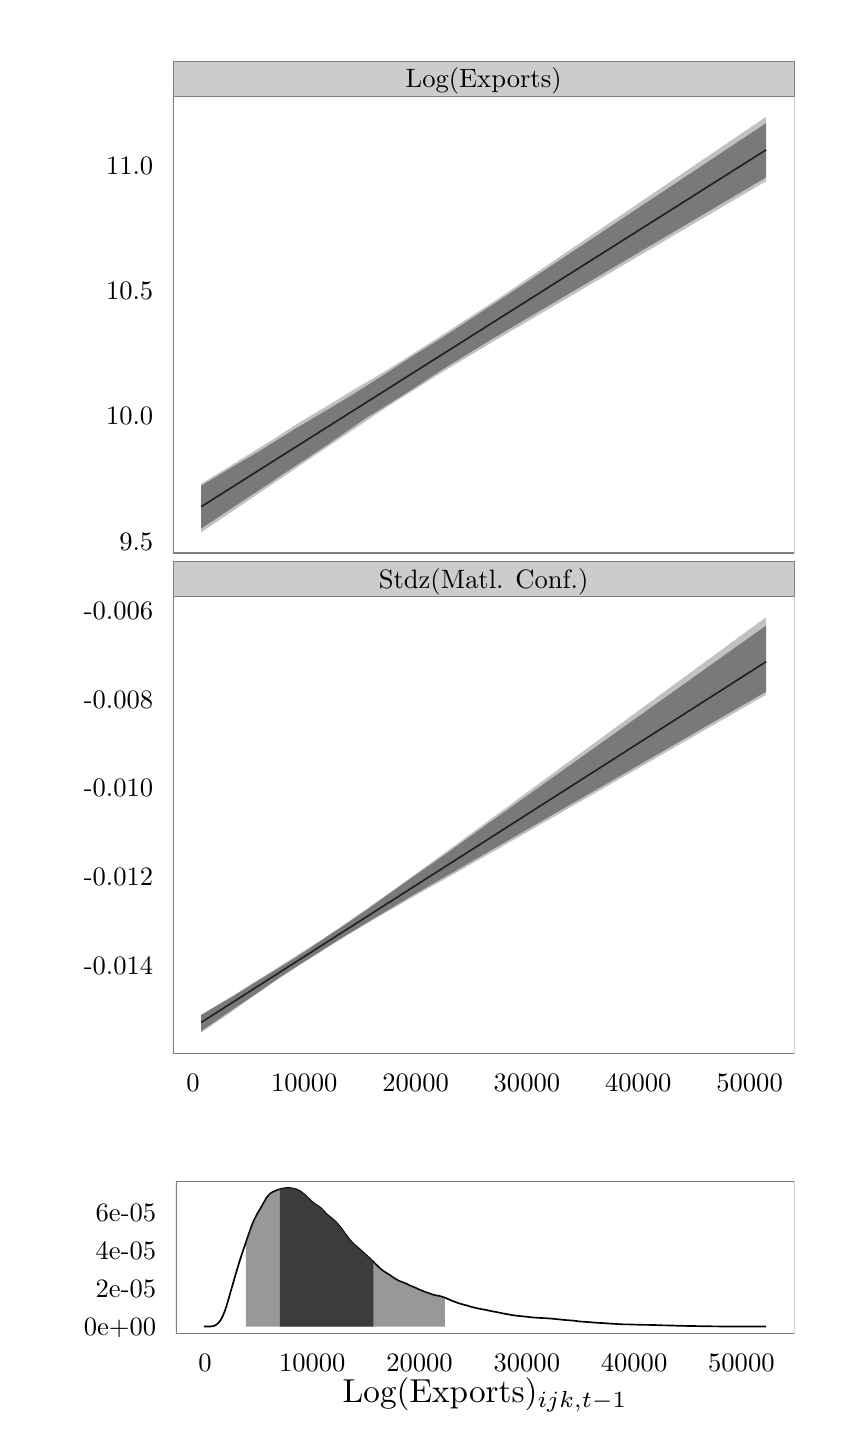
\begin{tikzpicture}[x=1pt,y=1pt]
\definecolor[named]{fillColor}{rgb}{1.00,1.00,1.00}
\path[use as bounding box,fill=fillColor,fill opacity=0.00] (0,0) rectangle (289.08,505.89);
\begin{scope}
\path[clip] (  0.00,101.18) rectangle (289.08,505.89);
\definecolor[named]{drawColor}{rgb}{1.00,1.00,1.00}
\definecolor[named]{fillColor}{rgb}{1.00,1.00,1.00}

\path[draw=drawColor,line width= 0.6pt,line join=round,line cap=round,fill=fillColor] (  0.00,101.18) rectangle (289.08,505.89);
\end{scope}
\begin{scope}
\path[clip] ( 52.48,316.03) rectangle (277.03,481.21);
\definecolor[named]{fillColor}{rgb}{1.00,1.00,1.00}

\path[fill=fillColor] ( 52.48,316.03) rectangle (277.03,481.21);
\definecolor[named]{drawColor}{rgb}{0.00,0.00,0.00}

\path[draw=drawColor,line width= 0.6pt,line join=round] ( 62.69,332.78) --
	( 74.63,340.32) --
	( 78.62,342.84) --
	( 81.91,344.92) --
	( 84.84,346.77) --
	( 87.67,348.56) --
	( 90.46,350.32) --
	( 93.24,352.07) --
	( 96.05,353.85) --
	( 98.99,355.71) --
	(102.12,357.69) --
	(105.41,359.76) --
	(108.96,362.01) --
	(112.89,364.49) --
	(117.50,367.40) --
	(122.89,370.81) --
	(129.68,375.10) --
	(138.40,380.61) --
	(149.97,387.91) --
	(168.80,399.81) --
	(266.83,461.73);
\definecolor[named]{fillColor}{rgb}{0.20,0.20,0.20}

\path[fill=fillColor,fill opacity=0.30] ( 62.69,341.05) --
	( 74.63,348.42) --
	( 78.62,350.88) --
	( 81.91,352.91) --
	( 84.84,354.72) --
	( 87.67,356.47) --
	( 90.46,358.27) --
	( 93.24,360.07) --
	( 96.05,361.89) --
	( 98.99,363.72) --
	(102.12,365.58) --
	(105.41,367.54) --
	(108.96,369.64) --
	(112.89,372.02) --
	(117.50,374.86) --
	(122.89,378.05) --
	(129.68,382.05) --
	(138.40,387.58) --
	(149.97,394.93) --
	(168.80,407.17) --
	(266.83,473.70) --
	(266.83,450.42) --
	(168.80,392.80) --
	(149.97,381.52) --
	(138.40,374.19) --
	(129.68,368.74) --
	(122.89,364.16) --
	(117.50,360.53) --
	(112.89,357.43) --
	(108.96,354.80) --
	(105.41,352.41) --
	(102.12,350.18) --
	( 98.99,348.07) --
	( 96.05,346.09) --
	( 93.24,344.18) --
	( 90.46,342.31) --
	( 87.67,340.43) --
	( 84.84,338.52) --
	( 81.91,336.52) --
	( 78.62,334.30) --
	( 74.63,331.61) --
	( 62.69,323.54) --
	cycle;
\definecolor[named]{fillColor}{rgb}{0.20,0.20,0.20}

\path[fill=fillColor,fill opacity=0.50] ( 62.69,340.35) --
	( 74.63,347.53) --
	( 78.62,349.86) --
	( 81.91,351.77) --
	( 84.84,353.59) --
	( 87.67,355.38) --
	( 90.46,357.08) --
	( 93.24,358.79) --
	( 96.05,360.55) --
	( 98.99,362.32) --
	(102.12,364.17) --
	(105.41,366.11) --
	(108.96,368.21) --
	(112.89,370.57) --
	(117.50,373.34) --
	(122.89,376.75) --
	(129.68,381.06) --
	(138.40,386.79) --
	(149.97,393.97) --
	(168.80,406.31) --
	(266.83,471.38) --
	(266.83,451.79) --
	(168.80,393.97) --
	(149.97,382.43) --
	(138.40,374.87) --
	(129.68,369.38) --
	(122.89,365.23) --
	(117.50,361.57) --
	(112.89,358.33) --
	(108.96,355.63) --
	(105.41,353.26) --
	(102.12,351.08) --
	( 98.99,349.00) --
	( 96.05,347.05) --
	( 93.24,345.18) --
	( 90.46,343.34) --
	( 87.67,341.45) --
	( 84.84,339.57) --
	( 81.91,337.64) --
	( 78.62,335.48) --
	( 74.63,332.83) --
	( 62.69,324.90) --
	cycle;
\definecolor[named]{drawColor}{rgb}{0.50,0.50,0.50}

\path[draw=drawColor,line width= 0.6pt,line join=round,line cap=round] ( 52.48,316.03) rectangle (277.03,481.21);
\end{scope}
\begin{scope}
\path[clip] ( 52.48,135.21) rectangle (277.03,300.39);
\definecolor[named]{fillColor}{rgb}{1.00,1.00,1.00}

\path[fill=fillColor] ( 52.48,135.21) rectangle (277.03,300.39);
\definecolor[named]{drawColor}{rgb}{0.00,0.00,0.00}

\path[draw=drawColor,line width= 0.6pt,line join=round] ( 62.69,146.43) --
	( 74.63,154.06) --
	( 78.62,156.61) --
	( 81.91,158.71) --
	( 84.84,160.58) --
	( 87.67,162.38) --
	( 90.46,164.16) --
	( 93.24,165.94) --
	( 96.05,167.73) --
	( 98.99,169.61) --
	(102.12,171.61) --
	(105.41,173.71) --
	(108.96,175.97) --
	(112.89,178.49) --
	(117.50,181.43) --
	(122.89,184.87) --
	(129.68,189.21) --
	(138.40,194.78) --
	(149.97,202.16) --
	(168.80,214.18) --
	(266.83,276.78);
\definecolor[named]{fillColor}{rgb}{0.20,0.20,0.20}

\path[fill=fillColor,fill opacity=0.30] ( 62.69,149.22) --
	( 74.63,156.36) --
	( 78.62,158.91) --
	( 81.91,161.01) --
	( 84.84,162.79) --
	( 87.67,164.51) --
	( 90.46,166.30) --
	( 93.24,168.09) --
	( 96.05,169.88) --
	( 98.99,171.75) --
	(102.12,173.79) --
	(105.41,175.81) --
	(108.96,178.19) --
	(112.89,180.78) --
	(117.50,184.01) --
	(122.89,187.82) --
	(129.68,192.48) --
	(138.40,198.79) --
	(149.97,207.21) --
	(168.80,221.02) --
	(266.83,292.88) --
	(266.83,264.86) --
	(168.80,208.48) --
	(149.97,197.79) --
	(138.40,191.33) --
	(129.68,186.30) --
	(122.89,182.32) --
	(117.50,179.17) --
	(112.89,176.33) --
	(108.96,174.00) --
	(105.41,171.67) --
	(102.12,169.59) --
	( 98.99,167.58) --
	( 96.05,165.68) --
	( 93.24,163.84) --
	( 90.46,162.03) --
	( 87.67,160.14) --
	( 84.84,158.13) --
	( 81.91,156.13) --
	( 78.62,153.83) --
	( 74.63,150.95) --
	( 62.69,142.72) --
	cycle;
\definecolor[named]{fillColor}{rgb}{0.20,0.20,0.20}

\path[fill=fillColor,fill opacity=0.50] ( 62.69,149.10) --
	( 74.63,156.17) --
	( 78.62,158.64) --
	( 81.91,160.67) --
	( 84.84,162.51) --
	( 87.67,164.26) --
	( 90.46,165.95) --
	( 93.24,167.65) --
	( 96.05,169.36) --
	( 98.99,171.30) --
	(102.12,173.32) --
	(105.41,175.58) --
	(108.96,177.94) --
	(112.89,180.56) --
	(117.50,183.68) --
	(122.89,187.34) --
	(129.68,192.28) --
	(138.40,198.43) --
	(149.97,206.49) --
	(168.80,220.03) --
	(266.83,289.84) --
	(266.83,265.95) --
	(168.80,209.42) --
	(149.97,198.58) --
	(138.40,191.93) --
	(129.68,186.71) --
	(122.89,182.69) --
	(117.50,179.39) --
	(112.89,176.59) --
	(108.96,174.07) --
	(105.41,171.86) --
	(102.12,169.76) --
	( 98.99,167.83) --
	( 96.05,165.94) --
	( 93.24,164.12) --
	( 90.46,162.32) --
	( 87.67,160.38) --
	( 84.84,158.37) --
	( 81.91,156.36) --
	( 78.62,154.15) --
	( 74.63,151.51) --
	( 62.69,143.30) --
	cycle;
\definecolor[named]{drawColor}{rgb}{0.50,0.50,0.50}

\path[draw=drawColor,line width= 0.6pt,line join=round,line cap=round] ( 52.48,135.21) rectangle (277.03,300.39);
\end{scope}
\begin{scope}
\path[clip] (  0.00,  0.00) rectangle (289.08,505.89);
\definecolor[named]{drawColor}{rgb}{0.50,0.50,0.50}
\definecolor[named]{fillColor}{rgb}{0.80,0.80,0.80}

\path[draw=drawColor,line width= 0.2pt,line join=round,line cap=round,fill=fillColor] ( 52.48,481.21) rectangle (277.03,493.84);
\definecolor[named]{drawColor}{rgb}{0.00,0.00,0.00}

\node[text=drawColor,anchor=base,inner sep=0pt, outer sep=0pt, scale=  0.96] at (164.76,484.22) {Log(Exports)};
\end{scope}
\begin{scope}
\path[clip] (  0.00,  0.00) rectangle (289.08,505.89);
\definecolor[named]{drawColor}{rgb}{0.50,0.50,0.50}
\definecolor[named]{fillColor}{rgb}{0.80,0.80,0.80}

\path[draw=drawColor,line width= 0.2pt,line join=round,line cap=round,fill=fillColor] ( 52.48,300.39) rectangle (277.03,313.02);
\definecolor[named]{drawColor}{rgb}{0.00,0.00,0.00}

\node[text=drawColor,anchor=base,inner sep=0pt, outer sep=0pt, scale=  0.96] at (164.76,303.40) {Stdz(Matl. Conf.)};
\end{scope}
\begin{scope}
\path[clip] (  0.00,  0.00) rectangle (289.08,505.89);
\definecolor[named]{drawColor}{rgb}{0.00,0.00,0.00}

\node[text=drawColor,anchor=base east,inner sep=0pt, outer sep=0pt, scale=  0.96] at ( 45.37,317.10) {9.5};

\node[text=drawColor,anchor=base east,inner sep=0pt, outer sep=0pt, scale=  0.96] at ( 45.37,362.35) {10.0};

\node[text=drawColor,anchor=base east,inner sep=0pt, outer sep=0pt, scale=  0.96] at ( 45.37,407.61) {10.5};

\node[text=drawColor,anchor=base east,inner sep=0pt, outer sep=0pt, scale=  0.96] at ( 45.37,452.87) {11.0};
\end{scope}
\begin{scope}
\path[clip] (  0.00,  0.00) rectangle (289.08,505.89);
\definecolor[named]{drawColor}{rgb}{0.00,0.00,0.00}

\node[text=drawColor,anchor=base east,inner sep=0pt, outer sep=0pt, scale=  0.96] at ( 45.37,163.87) {-0.014};

\node[text=drawColor,anchor=base east,inner sep=0pt, outer sep=0pt, scale=  0.96] at ( 45.37,195.93) {-0.012};

\node[text=drawColor,anchor=base east,inner sep=0pt, outer sep=0pt, scale=  0.96] at ( 45.37,227.98) {-0.010};

\node[text=drawColor,anchor=base east,inner sep=0pt, outer sep=0pt, scale=  0.96] at ( 45.37,260.04) {-0.008};

\node[text=drawColor,anchor=base east,inner sep=0pt, outer sep=0pt, scale=  0.96] at ( 45.37,292.09) {-0.006};
\end{scope}
\begin{scope}
\path[clip] (  0.00,  0.00) rectangle (289.08,505.89);
\definecolor[named]{drawColor}{rgb}{0.00,0.00,0.00}

\node[text=drawColor,anchor=base,inner sep=0pt, outer sep=0pt, scale=  0.96] at ( 59.73,121.49) {0};

\node[text=drawColor,anchor=base,inner sep=0pt, outer sep=0pt, scale=  0.96] at ( 99.95,121.49) {10000};

\node[text=drawColor,anchor=base,inner sep=0pt, outer sep=0pt, scale=  0.96] at (140.18,121.49) {20000};

\node[text=drawColor,anchor=base,inner sep=0pt, outer sep=0pt, scale=  0.96] at (180.40,121.49) {30000};

\node[text=drawColor,anchor=base,inner sep=0pt, outer sep=0pt, scale=  0.96] at (220.63,121.49) {40000};

\node[text=drawColor,anchor=base,inner sep=0pt, outer sep=0pt, scale=  0.96] at (260.86,121.49) {50000};
\end{scope}
\begin{scope}
\path[clip] (  0.00,  0.00) rectangle (289.08,101.18);
\definecolor[named]{drawColor}{rgb}{1.00,1.00,1.00}
\definecolor[named]{fillColor}{rgb}{1.00,1.00,1.00}

\path[draw=drawColor,line width= 0.6pt,line join=round,line cap=round,fill=fillColor] ( -0.00,  0.00) rectangle (289.08,101.18);
\end{scope}
\begin{scope}
\path[clip] ( 53.55, 34.03) rectangle (277.04, 89.13);
\definecolor[named]{fillColor}{rgb}{1.00,1.00,1.00}

\path[fill=fillColor] ( 53.55, 34.03) rectangle (277.04, 89.13);
\definecolor[named]{drawColor}{rgb}{0.00,0.00,0.00}

\path[draw=drawColor,line width= 0.6pt,line join=round] ( 63.71, 36.54) --
	( 64.11, 36.54) --
	( 64.50, 36.54) --
	( 64.90, 36.54) --
	( 65.30, 36.55) --
	( 65.70, 36.55) --
	( 66.09, 36.57) --
	( 66.49, 36.61) --
	( 66.89, 36.67) --
	( 67.29, 36.78) --
	( 67.68, 36.93) --
	( 68.08, 37.16) --
	( 68.48, 37.45) --
	( 68.88, 37.83) --
	( 69.27, 38.28) --
	( 69.67, 38.83) --
	( 70.07, 39.49) --
	( 70.47, 40.27) --
	( 70.86, 41.19) --
	( 71.26, 42.25) --
	( 71.66, 43.42) --
	( 72.06, 44.69) --
	( 72.46, 46.04) --
	( 72.85, 47.42) --
	( 73.25, 48.82) --
	( 73.65, 50.22) --
	( 74.05, 51.61) --
	( 74.44, 52.99) --
	( 74.84, 54.35) --
	( 75.24, 55.69) --
	( 75.64, 57.03) --
	( 76.03, 58.35) --
	( 76.43, 59.66) --
	( 76.83, 60.93) --
	( 77.23, 62.17) --
	( 77.62, 63.38) --
	( 78.02, 64.55) --
	( 78.42, 65.71) --
	( 78.82, 66.86) --
	( 79.21, 68.03) --
	( 79.61, 69.19) --
	( 80.01, 70.36) --
	( 80.41, 71.49) --
	( 80.80, 72.59) --
	( 81.20, 73.61) --
	( 81.60, 74.56) --
	( 82.00, 75.43) --
	( 82.40, 76.24) --
	( 82.79, 76.98) --
	( 83.19, 77.69) --
	( 83.59, 78.36) --
	( 83.99, 79.04) --
	( 84.38, 79.71) --
	( 84.78, 80.41) --
	( 85.18, 81.12) --
	( 85.58, 81.82) --
	( 85.97, 82.50) --
	( 86.37, 83.12) --
	( 86.77, 83.68) --
	( 87.17, 84.14) --
	( 87.56, 84.52) --
	( 87.96, 84.82) --
	( 88.36, 85.06) --
	( 88.76, 85.26) --
	( 89.15, 85.43) --
	( 89.55, 85.60) --
	( 89.95, 85.77) --
	( 90.35, 85.92) --
	( 90.74, 86.06) --
	( 91.14, 86.18) --
	( 91.54, 86.27) --
	( 91.94, 86.36) --
	( 92.33, 86.43) --
	( 92.73, 86.50) --
	( 93.13, 86.56) --
	( 93.53, 86.61) --
	( 93.93, 86.63) --
	( 94.32, 86.63) --
	( 94.72, 86.60) --
	( 95.12, 86.55) --
	( 95.52, 86.49) --
	( 95.91, 86.41) --
	( 96.31, 86.32) --
	( 96.71, 86.22) --
	( 97.11, 86.09) --
	( 97.50, 85.94) --
	( 97.90, 85.75) --
	( 98.30, 85.52) --
	( 98.70, 85.26) --
	( 99.09, 84.97) --
	( 99.49, 84.66) --
	( 99.89, 84.33) --
	(100.29, 83.97) --
	(100.68, 83.60) --
	(101.08, 83.21) --
	(101.48, 82.83) --
	(101.88, 82.44) --
	(102.27, 82.08) --
	(102.67, 81.72) --
	(103.07, 81.39) --
	(103.47, 81.08) --
	(103.86, 80.79) --
	(104.26, 80.51) --
	(104.66, 80.26) --
	(105.06, 80.00) --
	(105.46, 79.73) --
	(105.85, 79.42) --
	(106.25, 79.06) --
	(106.65, 78.65) --
	(107.05, 78.22) --
	(107.44, 77.78) --
	(107.84, 77.36) --
	(108.24, 76.98) --
	(108.64, 76.63) --
	(109.03, 76.31) --
	(109.43, 76.00) --
	(109.83, 75.68) --
	(110.23, 75.36) --
	(110.62, 75.02) --
	(111.02, 74.65) --
	(111.42, 74.26) --
	(111.82, 73.83) --
	(112.21, 73.38) --
	(112.61, 72.90) --
	(113.01, 72.39) --
	(113.41, 71.87) --
	(113.80, 71.34) --
	(114.20, 70.80) --
	(114.60, 70.26) --
	(115.00, 69.72) --
	(115.39, 69.18) --
	(115.79, 68.65) --
	(116.19, 68.15) --
	(116.59, 67.66) --
	(116.99, 67.21) --
	(117.38, 66.79) --
	(117.78, 66.40) --
	(118.18, 66.03) --
	(118.58, 65.69) --
	(118.97, 65.35) --
	(119.37, 65.02) --
	(119.77, 64.67) --
	(120.17, 64.31) --
	(120.56, 63.95) --
	(120.96, 63.59) --
	(121.36, 63.23) --
	(121.76, 62.87) --
	(122.15, 62.51) --
	(122.55, 62.15) --
	(122.95, 61.79) --
	(123.35, 61.44) --
	(123.74, 61.08) --
	(124.14, 60.70) --
	(124.54, 60.32) --
	(124.94, 59.92) --
	(125.33, 59.52) --
	(125.73, 59.12) --
	(126.13, 58.73) --
	(126.53, 58.34) --
	(126.93, 57.96) --
	(127.32, 57.59) --
	(127.72, 57.24) --
	(128.12, 56.91) --
	(128.52, 56.62) --
	(128.91, 56.36) --
	(129.31, 56.11) --
	(129.71, 55.88) --
	(130.11, 55.64) --
	(130.50, 55.39) --
	(130.90, 55.13) --
	(131.30, 54.85) --
	(131.70, 54.57) --
	(132.09, 54.29) --
	(132.49, 54.03) --
	(132.89, 53.78) --
	(133.29, 53.55) --
	(133.68, 53.34) --
	(134.08, 53.14) --
	(134.48, 52.96) --
	(134.88, 52.79) --
	(135.27, 52.63) --
	(135.67, 52.48) --
	(136.07, 52.33) --
	(136.47, 52.17) --
	(136.86, 52.00) --
	(137.26, 51.82) --
	(137.66, 51.62) --
	(138.06, 51.43) --
	(138.46, 51.25) --
	(138.85, 51.09) --
	(139.25, 50.93) --
	(139.65, 50.76) --
	(140.05, 50.59) --
	(140.44, 50.41) --
	(140.84, 50.22) --
	(141.24, 50.03) --
	(141.64, 49.85) --
	(142.03, 49.68) --
	(142.43, 49.52) --
	(142.83, 49.36) --
	(143.23, 49.21) --
	(143.62, 49.06) --
	(144.02, 48.92) --
	(144.42, 48.78) --
	(144.82, 48.64) --
	(145.21, 48.50) --
	(145.61, 48.36) --
	(146.01, 48.22) --
	(146.41, 48.09) --
	(146.80, 47.98) --
	(147.20, 47.89) --
	(147.60, 47.81) --
	(148.00, 47.73) --
	(148.39, 47.65) --
	(148.79, 47.57) --
	(149.19, 47.47) --
	(149.59, 47.37) --
	(149.99, 47.25) --
	(150.38, 47.12) --
	(150.78, 46.98) --
	(151.18, 46.82) --
	(151.58, 46.65) --
	(151.97, 46.47) --
	(152.37, 46.29) --
	(152.77, 46.11) --
	(153.17, 45.94) --
	(153.56, 45.78) --
	(153.96, 45.62) --
	(154.36, 45.47) --
	(154.76, 45.33) --
	(155.15, 45.18) --
	(155.55, 45.04) --
	(155.95, 44.91) --
	(156.35, 44.79) --
	(156.74, 44.67) --
	(157.14, 44.56) --
	(157.54, 44.46) --
	(157.94, 44.35) --
	(158.33, 44.25) --
	(158.73, 44.14) --
	(159.13, 44.02) --
	(159.53, 43.91) --
	(159.93, 43.79) --
	(160.32, 43.67) --
	(160.72, 43.56) --
	(161.12, 43.45) --
	(161.52, 43.35) --
	(161.91, 43.26) --
	(162.31, 43.18) --
	(162.71, 43.10) --
	(163.11, 43.02) --
	(163.50, 42.94) --
	(163.90, 42.86) --
	(164.30, 42.78) --
	(164.70, 42.71) --
	(165.09, 42.63) --
	(165.49, 42.55) --
	(165.89, 42.47) --
	(166.29, 42.38) --
	(166.68, 42.29) --
	(167.08, 42.21) --
	(167.48, 42.13) --
	(167.88, 42.05) --
	(168.27, 41.98) --
	(168.67, 41.91) --
	(169.07, 41.84) --
	(169.47, 41.76) --
	(169.86, 41.68) --
	(170.26, 41.59) --
	(170.66, 41.51) --
	(171.06, 41.43) --
	(171.46, 41.35) --
	(171.85, 41.27) --
	(172.25, 41.20) --
	(172.65, 41.13) --
	(173.05, 41.06) --
	(173.44, 40.98) --
	(173.84, 40.91) --
	(174.24, 40.84) --
	(174.64, 40.76) --
	(175.03, 40.69) --
	(175.43, 40.63) --
	(175.83, 40.57) --
	(176.23, 40.51) --
	(176.62, 40.46) --
	(177.02, 40.42) --
	(177.42, 40.38) --
	(177.82, 40.34) --
	(178.21, 40.30) --
	(178.61, 40.26) --
	(179.01, 40.22) --
	(179.41, 40.18) --
	(179.80, 40.13) --
	(180.20, 40.09) --
	(180.60, 40.04) --
	(181.00, 39.99) --
	(181.39, 39.94) --
	(181.79, 39.90) --
	(182.19, 39.86) --
	(182.59, 39.83) --
	(182.99, 39.80) --
	(183.38, 39.77) --
	(183.78, 39.74) --
	(184.18, 39.72) --
	(184.58, 39.69) --
	(184.97, 39.67) --
	(185.37, 39.65) --
	(185.77, 39.62) --
	(186.17, 39.60) --
	(186.56, 39.58) --
	(186.96, 39.56) --
	(187.36, 39.53) --
	(187.76, 39.51) --
	(188.15, 39.48) --
	(188.55, 39.45) --
	(188.95, 39.43) --
	(189.35, 39.40) --
	(189.74, 39.36) --
	(190.14, 39.33) --
	(190.54, 39.28) --
	(190.94, 39.24) --
	(191.33, 39.20) --
	(191.73, 39.16) --
	(192.13, 39.12) --
	(192.53, 39.07) --
	(192.92, 39.03) --
	(193.32, 38.99) --
	(193.72, 38.95) --
	(194.12, 38.91) --
	(194.52, 38.87) --
	(194.91, 38.84) --
	(195.31, 38.81) --
	(195.71, 38.79) --
	(196.11, 38.76) --
	(196.50, 38.74) --
	(196.90, 38.71) --
	(197.30, 38.67) --
	(197.70, 38.62) --
	(198.09, 38.57) --
	(198.49, 38.51) --
	(198.89, 38.45) --
	(199.29, 38.40) --
	(199.68, 38.36) --
	(200.08, 38.33) --
	(200.48, 38.30) --
	(200.88, 38.27) --
	(201.27, 38.25) --
	(201.67, 38.22) --
	(202.07, 38.19) --
	(202.47, 38.17) --
	(202.86, 38.14) --
	(203.26, 38.10) --
	(203.66, 38.07) --
	(204.06, 38.04) --
	(204.46, 38.00) --
	(204.85, 37.97) --
	(205.25, 37.94) --
	(205.65, 37.91) --
	(206.05, 37.88) --
	(206.44, 37.86) --
	(206.84, 37.84) --
	(207.24, 37.83) --
	(207.64, 37.81) --
	(208.03, 37.78) --
	(208.43, 37.76) --
	(208.83, 37.73) --
	(209.23, 37.69) --
	(209.62, 37.66) --
	(210.02, 37.63) --
	(210.42, 37.61) --
	(210.82, 37.58) --
	(211.21, 37.56) --
	(211.61, 37.54) --
	(212.01, 37.52) --
	(212.41, 37.49) --
	(212.80, 37.47) --
	(213.20, 37.45) --
	(213.60, 37.42) --
	(214.00, 37.39) --
	(214.39, 37.37) --
	(214.79, 37.35) --
	(215.19, 37.34) --
	(215.59, 37.33) --
	(215.99, 37.33) --
	(216.38, 37.33) --
	(216.78, 37.33) --
	(217.18, 37.32) --
	(217.58, 37.30) --
	(217.97, 37.29) --
	(218.37, 37.27) --
	(218.77, 37.26) --
	(219.17, 37.24) --
	(219.56, 37.23) --
	(219.96, 37.23) --
	(220.36, 37.22) --
	(220.76, 37.21) --
	(221.15, 37.20) --
	(221.55, 37.18) --
	(221.95, 37.17) --
	(222.35, 37.16) --
	(222.74, 37.16) --
	(223.14, 37.15) --
	(223.54, 37.15) --
	(223.94, 37.14) --
	(224.33, 37.13) --
	(224.73, 37.13) --
	(225.13, 37.12) --
	(225.53, 37.11) --
	(225.92, 37.10) --
	(226.32, 37.09) --
	(226.72, 37.08) --
	(227.12, 37.07) --
	(227.52, 37.05) --
	(227.91, 37.04) --
	(228.31, 37.02) --
	(228.71, 37.00) --
	(229.11, 36.99) --
	(229.50, 36.97) --
	(229.90, 36.96) --
	(230.30, 36.96) --
	(230.70, 36.95) --
	(231.09, 36.95) --
	(231.49, 36.94) --
	(231.89, 36.94) --
	(232.29, 36.93) --
	(232.68, 36.92) --
	(233.08, 36.90) --
	(233.48, 36.89) --
	(233.88, 36.88) --
	(234.27, 36.86) --
	(234.67, 36.85) --
	(235.07, 36.84) --
	(235.47, 36.83) --
	(235.86, 36.82) --
	(236.26, 36.81) --
	(236.66, 36.80) --
	(237.06, 36.79) --
	(237.45, 36.78) --
	(237.85, 36.77) --
	(238.25, 36.76) --
	(238.65, 36.75) --
	(239.05, 36.75) --
	(239.44, 36.75) --
	(239.84, 36.75) --
	(240.24, 36.74) --
	(240.64, 36.73) --
	(241.03, 36.72) --
	(241.43, 36.71) --
	(241.83, 36.70) --
	(242.23, 36.69) --
	(242.62, 36.68) --
	(243.02, 36.67) --
	(243.42, 36.66) --
	(243.82, 36.66) --
	(244.21, 36.65) --
	(244.61, 36.64) --
	(245.01, 36.63) --
	(245.41, 36.63) --
	(245.80, 36.63) --
	(246.20, 36.62) --
	(246.60, 36.62) --
	(247.00, 36.62) --
	(247.39, 36.61) --
	(247.79, 36.61) --
	(248.19, 36.61) --
	(248.59, 36.60) --
	(248.99, 36.60) --
	(249.38, 36.59) --
	(249.78, 36.59) --
	(250.18, 36.58) --
	(250.58, 36.58) --
	(250.97, 36.58) --
	(251.37, 36.57) --
	(251.77, 36.57) --
	(252.17, 36.56) --
	(252.56, 36.56) --
	(252.96, 36.56) --
	(253.36, 36.56) --
	(253.76, 36.56) --
	(254.15, 36.56) --
	(254.55, 36.56) --
	(254.95, 36.56) --
	(255.35, 36.56) --
	(255.74, 36.56) --
	(256.14, 36.55) --
	(256.54, 36.55) --
	(256.94, 36.55) --
	(257.33, 36.55) --
	(257.73, 36.55) --
	(258.13, 36.55) --
	(258.53, 36.54) --
	(258.92, 36.54) --
	(259.32, 36.54) --
	(259.72, 36.54) --
	(260.12, 36.54) --
	(260.52, 36.54) --
	(260.91, 36.54) --
	(261.31, 36.54) --
	(261.71, 36.54) --
	(262.11, 36.54) --
	(262.50, 36.54) --
	(262.90, 36.54) --
	(263.30, 36.54) --
	(263.70, 36.54) --
	(264.09, 36.54) --
	(264.49, 36.54) --
	(264.89, 36.54) --
	(265.29, 36.54) --
	(265.68, 36.54) --
	(266.08, 36.54) --
	(266.48, 36.54) --
	(266.88, 36.54);
\definecolor[named]{fillColor}{rgb}{0.20,0.20,0.20}

\path[fill=fillColor,fill opacity=0.50] ( 78.82, 66.86) --
	( 79.21, 68.03) --
	( 79.61, 69.19) --
	( 80.01, 70.36) --
	( 80.41, 71.49) --
	( 80.80, 72.59) --
	( 81.20, 73.61) --
	( 81.60, 74.56) --
	( 82.00, 75.43) --
	( 82.40, 76.24) --
	( 82.79, 76.98) --
	( 83.19, 77.69) --
	( 83.59, 78.36) --
	( 83.99, 79.04) --
	( 84.38, 79.71) --
	( 84.78, 80.41) --
	( 85.18, 81.12) --
	( 85.58, 81.82) --
	( 85.97, 82.50) --
	( 86.37, 83.12) --
	( 86.77, 83.68) --
	( 87.17, 84.14) --
	( 87.56, 84.52) --
	( 87.96, 84.82) --
	( 88.36, 85.06) --
	( 88.76, 85.26) --
	( 89.15, 85.43) --
	( 89.55, 85.60) --
	( 89.95, 85.77) --
	( 90.35, 85.92) --
	( 90.74, 86.06) --
	( 91.14, 86.18) --
	( 91.54, 86.27) --
	( 91.94, 86.36) --
	( 92.33, 86.43) --
	( 92.73, 86.50) --
	( 93.13, 86.56) --
	( 93.53, 86.61) --
	( 93.93, 86.63) --
	( 94.32, 86.63) --
	( 94.72, 86.60) --
	( 95.12, 86.55) --
	( 95.52, 86.49) --
	( 95.91, 86.41) --
	( 96.31, 86.32) --
	( 96.71, 86.22) --
	( 97.11, 86.09) --
	( 97.50, 85.94) --
	( 97.90, 85.75) --
	( 98.30, 85.52) --
	( 98.70, 85.26) --
	( 99.09, 84.97) --
	( 99.49, 84.66) --
	( 99.89, 84.33) --
	(100.29, 83.97) --
	(100.68, 83.60) --
	(101.08, 83.21) --
	(101.48, 82.83) --
	(101.88, 82.44) --
	(102.27, 82.08) --
	(102.67, 81.72) --
	(103.07, 81.39) --
	(103.47, 81.08) --
	(103.86, 80.79) --
	(104.26, 80.51) --
	(104.66, 80.26) --
	(105.06, 80.00) --
	(105.46, 79.73) --
	(105.85, 79.42) --
	(106.25, 79.06) --
	(106.65, 78.65) --
	(107.05, 78.22) --
	(107.44, 77.78) --
	(107.84, 77.36) --
	(108.24, 76.98) --
	(108.64, 76.63) --
	(109.03, 76.31) --
	(109.43, 76.00) --
	(109.83, 75.68) --
	(110.23, 75.36) --
	(110.62, 75.02) --
	(111.02, 74.65) --
	(111.42, 74.26) --
	(111.82, 73.83) --
	(112.21, 73.38) --
	(112.61, 72.90) --
	(113.01, 72.39) --
	(113.41, 71.87) --
	(113.80, 71.34) --
	(114.20, 70.80) --
	(114.60, 70.26) --
	(115.00, 69.72) --
	(115.39, 69.18) --
	(115.79, 68.65) --
	(116.19, 68.15) --
	(116.59, 67.66) --
	(116.99, 67.21) --
	(117.38, 66.79) --
	(117.78, 66.40) --
	(118.18, 66.03) --
	(118.58, 65.69) --
	(118.97, 65.35) --
	(119.37, 65.02) --
	(119.77, 64.67) --
	(120.17, 64.31) --
	(120.56, 63.95) --
	(120.96, 63.59) --
	(121.36, 63.23) --
	(121.76, 62.87) --
	(122.15, 62.51) --
	(122.55, 62.15) --
	(122.95, 61.79) --
	(123.35, 61.44) --
	(123.74, 61.08) --
	(124.14, 60.70) --
	(124.54, 60.32) --
	(124.94, 59.92) --
	(125.33, 59.52) --
	(125.73, 59.12) --
	(126.13, 58.73) --
	(126.53, 58.34) --
	(126.93, 57.96) --
	(127.32, 57.59) --
	(127.72, 57.24) --
	(128.12, 56.91) --
	(128.52, 56.62) --
	(128.91, 56.36) --
	(129.31, 56.11) --
	(129.71, 55.88) --
	(130.11, 55.64) --
	(130.50, 55.39) --
	(130.90, 55.13) --
	(131.30, 54.85) --
	(131.70, 54.57) --
	(132.09, 54.29) --
	(132.49, 54.03) --
	(132.89, 53.78) --
	(133.29, 53.55) --
	(133.68, 53.34) --
	(134.08, 53.14) --
	(134.48, 52.96) --
	(134.88, 52.79) --
	(135.27, 52.63) --
	(135.67, 52.48) --
	(136.07, 52.33) --
	(136.47, 52.17) --
	(136.86, 52.00) --
	(137.26, 51.82) --
	(137.66, 51.62) --
	(138.06, 51.43) --
	(138.46, 51.25) --
	(138.85, 51.09) --
	(139.25, 50.93) --
	(139.65, 50.76) --
	(140.05, 50.59) --
	(140.44, 50.41) --
	(140.84, 50.22) --
	(141.24, 50.03) --
	(141.64, 49.85) --
	(142.03, 49.68) --
	(142.43, 49.52) --
	(142.83, 49.36) --
	(143.23, 49.21) --
	(143.62, 49.06) --
	(144.02, 48.92) --
	(144.42, 48.78) --
	(144.82, 48.64) --
	(145.21, 48.50) --
	(145.61, 48.36) --
	(146.01, 48.22) --
	(146.41, 48.09) --
	(146.80, 47.98) --
	(147.20, 47.89) --
	(147.60, 47.81) --
	(148.00, 47.73) --
	(148.39, 47.65) --
	(148.79, 47.57) --
	(149.19, 47.47) --
	(149.59, 47.37) --
	(149.99, 47.25) --
	(150.38, 47.12) --
	(150.78, 46.98) --
	(150.78, 36.54) --
	(150.38, 36.54) --
	(149.99, 36.54) --
	(149.59, 36.54) --
	(149.19, 36.54) --
	(148.79, 36.54) --
	(148.39, 36.54) --
	(148.00, 36.54) --
	(147.60, 36.54) --
	(147.20, 36.54) --
	(146.80, 36.54) --
	(146.41, 36.54) --
	(146.01, 36.54) --
	(145.61, 36.54) --
	(145.21, 36.54) --
	(144.82, 36.54) --
	(144.42, 36.54) --
	(144.02, 36.54) --
	(143.62, 36.54) --
	(143.23, 36.54) --
	(142.83, 36.54) --
	(142.43, 36.54) --
	(142.03, 36.54) --
	(141.64, 36.54) --
	(141.24, 36.54) --
	(140.84, 36.54) --
	(140.44, 36.54) --
	(140.05, 36.54) --
	(139.65, 36.54) --
	(139.25, 36.54) --
	(138.85, 36.54) --
	(138.46, 36.54) --
	(138.06, 36.54) --
	(137.66, 36.54) --
	(137.26, 36.54) --
	(136.86, 36.54) --
	(136.47, 36.54) --
	(136.07, 36.54) --
	(135.67, 36.54) --
	(135.27, 36.54) --
	(134.88, 36.54) --
	(134.48, 36.54) --
	(134.08, 36.54) --
	(133.68, 36.54) --
	(133.29, 36.54) --
	(132.89, 36.54) --
	(132.49, 36.54) --
	(132.09, 36.54) --
	(131.70, 36.54) --
	(131.30, 36.54) --
	(130.90, 36.54) --
	(130.50, 36.54) --
	(130.11, 36.54) --
	(129.71, 36.54) --
	(129.31, 36.54) --
	(128.91, 36.54) --
	(128.52, 36.54) --
	(128.12, 36.54) --
	(127.72, 36.54) --
	(127.32, 36.54) --
	(126.93, 36.54) --
	(126.53, 36.54) --
	(126.13, 36.54) --
	(125.73, 36.54) --
	(125.33, 36.54) --
	(124.94, 36.54) --
	(124.54, 36.54) --
	(124.14, 36.54) --
	(123.74, 36.54) --
	(123.35, 36.54) --
	(122.95, 36.54) --
	(122.55, 36.54) --
	(122.15, 36.54) --
	(121.76, 36.54) --
	(121.36, 36.54) --
	(120.96, 36.54) --
	(120.56, 36.54) --
	(120.17, 36.54) --
	(119.77, 36.54) --
	(119.37, 36.54) --
	(118.97, 36.54) --
	(118.58, 36.54) --
	(118.18, 36.54) --
	(117.78, 36.54) --
	(117.38, 36.54) --
	(116.99, 36.54) --
	(116.59, 36.54) --
	(116.19, 36.54) --
	(115.79, 36.54) --
	(115.39, 36.54) --
	(115.00, 36.54) --
	(114.60, 36.54) --
	(114.20, 36.54) --
	(113.80, 36.54) --
	(113.41, 36.54) --
	(113.01, 36.54) --
	(112.61, 36.54) --
	(112.21, 36.54) --
	(111.82, 36.54) --
	(111.42, 36.54) --
	(111.02, 36.54) --
	(110.62, 36.54) --
	(110.23, 36.54) --
	(109.83, 36.54) --
	(109.43, 36.54) --
	(109.03, 36.54) --
	(108.64, 36.54) --
	(108.24, 36.54) --
	(107.84, 36.54) --
	(107.44, 36.54) --
	(107.05, 36.54) --
	(106.65, 36.54) --
	(106.25, 36.54) --
	(105.85, 36.54) --
	(105.46, 36.54) --
	(105.06, 36.54) --
	(104.66, 36.54) --
	(104.26, 36.54) --
	(103.86, 36.54) --
	(103.47, 36.54) --
	(103.07, 36.54) --
	(102.67, 36.54) --
	(102.27, 36.54) --
	(101.88, 36.54) --
	(101.48, 36.54) --
	(101.08, 36.54) --
	(100.68, 36.54) --
	(100.29, 36.54) --
	( 99.89, 36.54) --
	( 99.49, 36.54) --
	( 99.09, 36.54) --
	( 98.70, 36.54) --
	( 98.30, 36.54) --
	( 97.90, 36.54) --
	( 97.50, 36.54) --
	( 97.11, 36.54) --
	( 96.71, 36.54) --
	( 96.31, 36.54) --
	( 95.91, 36.54) --
	( 95.52, 36.54) --
	( 95.12, 36.54) --
	( 94.72, 36.54) --
	( 94.32, 36.54) --
	( 93.93, 36.54) --
	( 93.53, 36.54) --
	( 93.13, 36.54) --
	( 92.73, 36.54) --
	( 92.33, 36.54) --
	( 91.94, 36.54) --
	( 91.54, 36.54) --
	( 91.14, 36.54) --
	( 90.74, 36.54) --
	( 90.35, 36.54) --
	( 89.95, 36.54) --
	( 89.55, 36.54) --
	( 89.15, 36.54) --
	( 88.76, 36.54) --
	( 88.36, 36.54) --
	( 87.96, 36.54) --
	( 87.56, 36.54) --
	( 87.17, 36.54) --
	( 86.77, 36.54) --
	( 86.37, 36.54) --
	( 85.97, 36.54) --
	( 85.58, 36.54) --
	( 85.18, 36.54) --
	( 84.78, 36.54) --
	( 84.38, 36.54) --
	( 83.99, 36.54) --
	( 83.59, 36.54) --
	( 83.19, 36.54) --
	( 82.79, 36.54) --
	( 82.40, 36.54) --
	( 82.00, 36.54) --
	( 81.60, 36.54) --
	( 81.20, 36.54) --
	( 80.80, 36.54) --
	( 80.41, 36.54) --
	( 80.01, 36.54) --
	( 79.61, 36.54) --
	( 79.21, 36.54) --
	( 78.82, 36.54) --
	cycle;
\definecolor[named]{fillColor}{rgb}{0.20,0.20,0.20}

\path[fill=fillColor,fill opacity=0.90] ( 91.14, 86.18) --
	( 91.54, 86.27) --
	( 91.94, 86.36) --
	( 92.33, 86.43) --
	( 92.73, 86.50) --
	( 93.13, 86.56) --
	( 93.53, 86.61) --
	( 93.93, 86.63) --
	( 94.32, 86.63) --
	( 94.72, 86.60) --
	( 95.12, 86.55) --
	( 95.52, 86.49) --
	( 95.91, 86.41) --
	( 96.31, 86.32) --
	( 96.71, 86.22) --
	( 97.11, 86.09) --
	( 97.50, 85.94) --
	( 97.90, 85.75) --
	( 98.30, 85.52) --
	( 98.70, 85.26) --
	( 99.09, 84.97) --
	( 99.49, 84.66) --
	( 99.89, 84.33) --
	(100.29, 83.97) --
	(100.68, 83.60) --
	(101.08, 83.21) --
	(101.48, 82.83) --
	(101.88, 82.44) --
	(102.27, 82.08) --
	(102.67, 81.72) --
	(103.07, 81.39) --
	(103.47, 81.08) --
	(103.86, 80.79) --
	(104.26, 80.51) --
	(104.66, 80.26) --
	(105.06, 80.00) --
	(105.46, 79.73) --
	(105.85, 79.42) --
	(106.25, 79.06) --
	(106.65, 78.65) --
	(107.05, 78.22) --
	(107.44, 77.78) --
	(107.84, 77.36) --
	(108.24, 76.98) --
	(108.64, 76.63) --
	(109.03, 76.31) --
	(109.43, 76.00) --
	(109.83, 75.68) --
	(110.23, 75.36) --
	(110.62, 75.02) --
	(111.02, 74.65) --
	(111.42, 74.26) --
	(111.82, 73.83) --
	(112.21, 73.38) --
	(112.61, 72.90) --
	(113.01, 72.39) --
	(113.41, 71.87) --
	(113.80, 71.34) --
	(114.20, 70.80) --
	(114.60, 70.26) --
	(115.00, 69.72) --
	(115.39, 69.18) --
	(115.79, 68.65) --
	(116.19, 68.15) --
	(116.59, 67.66) --
	(116.99, 67.21) --
	(117.38, 66.79) --
	(117.78, 66.40) --
	(118.18, 66.03) --
	(118.58, 65.69) --
	(118.97, 65.35) --
	(119.37, 65.02) --
	(119.77, 64.67) --
	(120.17, 64.31) --
	(120.56, 63.95) --
	(120.96, 63.59) --
	(121.36, 63.23) --
	(121.76, 62.87) --
	(122.15, 62.51) --
	(122.55, 62.15) --
	(122.95, 61.79) --
	(123.35, 61.44) --
	(123.74, 61.08) --
	(124.14, 60.70) --
	(124.54, 60.32) --
	(124.94, 59.92) --
	(124.94, 36.54) --
	(124.54, 36.54) --
	(124.14, 36.54) --
	(123.74, 36.54) --
	(123.35, 36.54) --
	(122.95, 36.54) --
	(122.55, 36.54) --
	(122.15, 36.54) --
	(121.76, 36.54) --
	(121.36, 36.54) --
	(120.96, 36.54) --
	(120.56, 36.54) --
	(120.17, 36.54) --
	(119.77, 36.54) --
	(119.37, 36.54) --
	(118.97, 36.54) --
	(118.58, 36.54) --
	(118.18, 36.54) --
	(117.78, 36.54) --
	(117.38, 36.54) --
	(116.99, 36.54) --
	(116.59, 36.54) --
	(116.19, 36.54) --
	(115.79, 36.54) --
	(115.39, 36.54) --
	(115.00, 36.54) --
	(114.60, 36.54) --
	(114.20, 36.54) --
	(113.80, 36.54) --
	(113.41, 36.54) --
	(113.01, 36.54) --
	(112.61, 36.54) --
	(112.21, 36.54) --
	(111.82, 36.54) --
	(111.42, 36.54) --
	(111.02, 36.54) --
	(110.62, 36.54) --
	(110.23, 36.54) --
	(109.83, 36.54) --
	(109.43, 36.54) --
	(109.03, 36.54) --
	(108.64, 36.54) --
	(108.24, 36.54) --
	(107.84, 36.54) --
	(107.44, 36.54) --
	(107.05, 36.54) --
	(106.65, 36.54) --
	(106.25, 36.54) --
	(105.85, 36.54) --
	(105.46, 36.54) --
	(105.06, 36.54) --
	(104.66, 36.54) --
	(104.26, 36.54) --
	(103.86, 36.54) --
	(103.47, 36.54) --
	(103.07, 36.54) --
	(102.67, 36.54) --
	(102.27, 36.54) --
	(101.88, 36.54) --
	(101.48, 36.54) --
	(101.08, 36.54) --
	(100.68, 36.54) --
	(100.29, 36.54) --
	( 99.89, 36.54) --
	( 99.49, 36.54) --
	( 99.09, 36.54) --
	( 98.70, 36.54) --
	( 98.30, 36.54) --
	( 97.90, 36.54) --
	( 97.50, 36.54) --
	( 97.11, 36.54) --
	( 96.71, 36.54) --
	( 96.31, 36.54) --
	( 95.91, 36.54) --
	( 95.52, 36.54) --
	( 95.12, 36.54) --
	( 94.72, 36.54) --
	( 94.32, 36.54) --
	( 93.93, 36.54) --
	( 93.53, 36.54) --
	( 93.13, 36.54) --
	( 92.73, 36.54) --
	( 92.33, 36.54) --
	( 91.94, 36.54) --
	( 91.54, 36.54) --
	( 91.14, 36.54) --
	cycle;
\definecolor[named]{drawColor}{rgb}{0.50,0.50,0.50}

\path[draw=drawColor,line width= 0.6pt,line join=round,line cap=round] ( 53.55, 34.03) rectangle (277.04, 89.13);
\end{scope}
\begin{scope}
\path[clip] (  0.00,  0.00) rectangle (289.08,505.89);
\definecolor[named]{drawColor}{rgb}{0.00,0.00,0.00}

\node[text=drawColor,anchor=base east,inner sep=0pt, outer sep=0pt, scale=  0.96] at ( 46.44, 33.23) {0e+00};

\node[text=drawColor,anchor=base east,inner sep=0pt, outer sep=0pt, scale=  0.96] at ( 46.44, 47.05) {2e-05};

\node[text=drawColor,anchor=base east,inner sep=0pt, outer sep=0pt, scale=  0.96] at ( 46.44, 60.86) {4e-05};

\node[text=drawColor,anchor=base east,inner sep=0pt, outer sep=0pt, scale=  0.96] at ( 46.44, 74.67) {6e-05};
\end{scope}
\begin{scope}
\path[clip] (  0.00,  0.00) rectangle (289.08,505.89);
\definecolor[named]{drawColor}{rgb}{0.00,0.00,0.00}

\node[text=drawColor,anchor=base,inner sep=0pt, outer sep=0pt, scale=  0.96] at ( 64.08, 20.31) {0};

\node[text=drawColor,anchor=base,inner sep=0pt, outer sep=0pt, scale=  0.96] at (102.84, 20.31) {10000};

\node[text=drawColor,anchor=base,inner sep=0pt, outer sep=0pt, scale=  0.96] at (141.61, 20.31) {20000};

\node[text=drawColor,anchor=base,inner sep=0pt, outer sep=0pt, scale=  0.96] at (180.37, 20.31) {30000};

\node[text=drawColor,anchor=base,inner sep=0pt, outer sep=0pt, scale=  0.96] at (219.13, 20.31) {40000};

\node[text=drawColor,anchor=base,inner sep=0pt, outer sep=0pt, scale=  0.96] at (257.89, 20.31) {50000};
\end{scope}
\begin{scope}
\path[clip] (  0.00,  0.00) rectangle (289.08,505.89);
\definecolor[named]{drawColor}{rgb}{0.00,0.00,0.00}

\node[text=drawColor,anchor=base,inner sep=0pt, outer sep=0pt, scale=  1.20] at (165.29,  9.03) {Log(Exports)$_{ijk, t-1}$};
\end{scope}
\end{tikzpicture}
}  
    \end{tabular}
  \end{figure}
}
%%%%%%%%%%%%%%%%%%%%%%%%%%%%%%%%%%%%%%%%%%%%%%%%%%%%%%%%%%%%

%%%%%%%%%%%%%%%%%%%%%%%%%%%%%%%%%%%%%%%%%%%%%%%%%%%%%%%%%%%%
\frame
{
\frametitle{Endog. Effects of Std(Matl. Conf.)}
  \vspace{-.3in}
  \begin{figure}[ht]
  \centering
    \begin{tabular}{ccc}
      \hspace{-.63in}
      \resizebox{.38\textwidth}{!}{% Created by tikzDevice version 0.7.0 on 2015-07-01 02:11:43
% !TEX encoding = UTF-8 Unicode
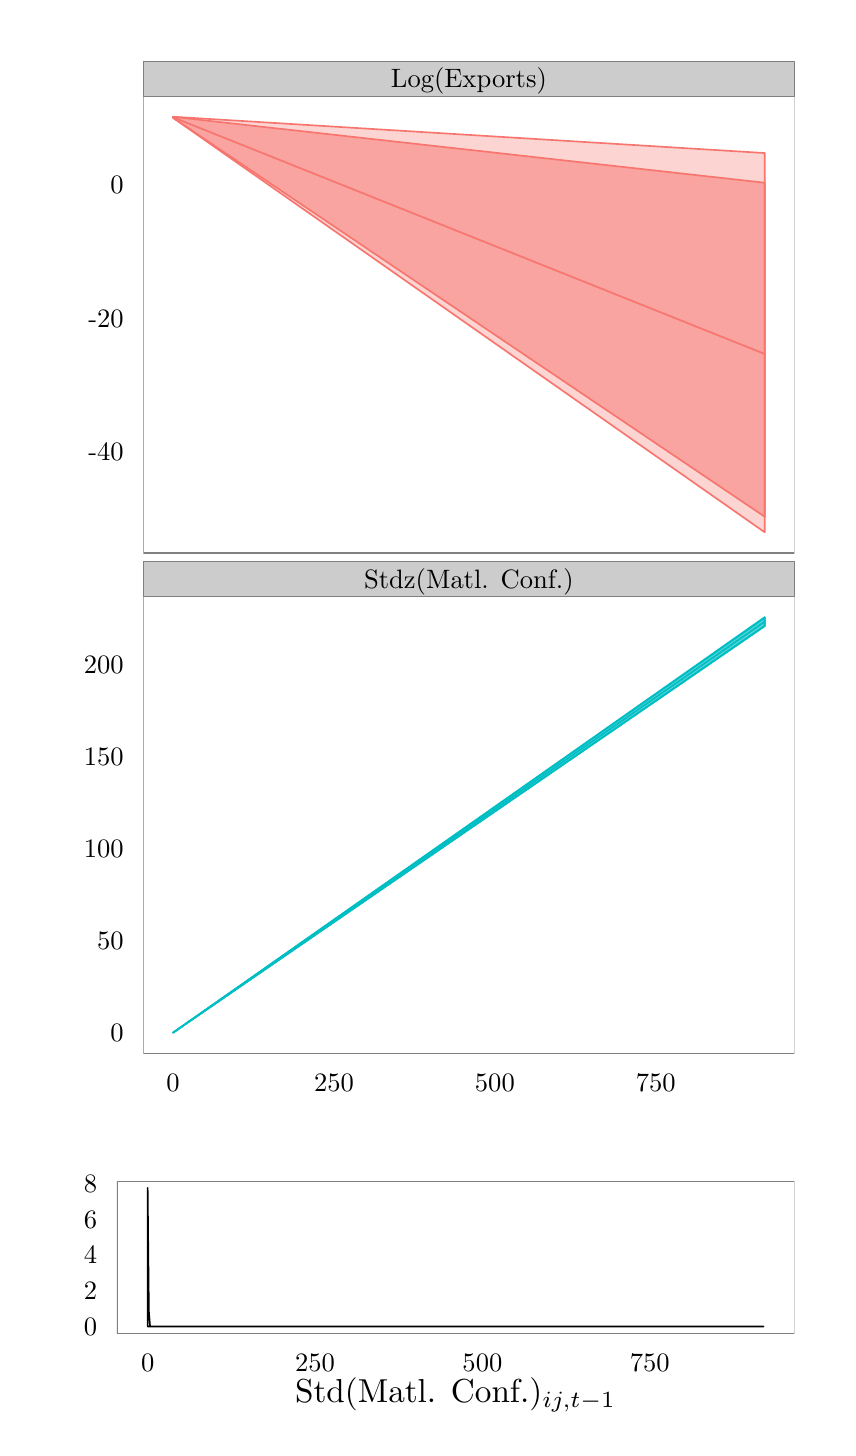
\begin{tikzpicture}[x=1pt,y=1pt]
\definecolor[named]{fillColor}{rgb}{1.00,1.00,1.00}
\path[use as bounding box,fill=fillColor,fill opacity=0.00] (0,0) rectangle (289.08,505.89);
\begin{scope}
\path[clip] (  0.00,101.18) rectangle (289.08,505.89);
\definecolor[named]{drawColor}{rgb}{1.00,1.00,1.00}
\definecolor[named]{fillColor}{rgb}{1.00,1.00,1.00}

\path[draw=drawColor,line width= 0.6pt,line join=round,line cap=round,fill=fillColor] ( -0.00,101.18) rectangle (289.08,505.89);
\end{scope}
\begin{scope}
\path[clip] ( 41.82,316.03) rectangle (277.04,481.21);
\definecolor[named]{fillColor}{rgb}{1.00,1.00,1.00}

\path[fill=fillColor] ( 41.82,316.03) rectangle (277.03,481.21);
\definecolor[named]{drawColor}{rgb}{0.97,0.46,0.43}

\path[draw=drawColor,line width= 0.6pt,line join=round] ( 52.51,473.50) --
	(266.34,387.98);
\definecolor[named]{fillColor}{rgb}{0.97,0.46,0.43}

\path[draw=drawColor,line width= 0.6pt,line join=round,line cap=round,fill=fillColor,fill opacity=0.30] ( 52.51,473.70) --
	(266.34,460.58) --
	(266.34,323.54) --
	( 52.51,473.31) --
	cycle;
\definecolor[named]{fillColor}{rgb}{0.97,0.46,0.43}

\path[draw=drawColor,line width= 0.6pt,line join=round,line cap=round,fill=fillColor,fill opacity=0.50] ( 52.51,473.66) --
	(266.34,449.86) --
	(266.34,329.16) --
	( 52.51,473.33) --
	cycle;
\definecolor[named]{drawColor}{rgb}{0.50,0.50,0.50}

\path[draw=drawColor,line width= 0.6pt,line join=round,line cap=round] ( 41.82,316.03) rectangle (277.03,481.21);
\end{scope}
\begin{scope}
\path[clip] ( 41.82,135.21) rectangle (277.04,300.39);
\definecolor[named]{fillColor}{rgb}{1.00,1.00,1.00}

\path[fill=fillColor] ( 41.82,135.21) rectangle (277.03,300.39);
\definecolor[named]{drawColor}{rgb}{0.00,0.75,0.77}

\path[draw=drawColor,line width= 0.6pt,line join=round] ( 52.51,142.72) --
	(266.34,291.27);
\definecolor[named]{fillColor}{rgb}{0.00,0.75,0.77}

\path[draw=drawColor,line width= 0.6pt,line join=round,line cap=round,fill=fillColor,fill opacity=0.30] ( 52.51,142.72) --
	(266.34,292.88) --
	(266.34,289.62) --
	( 52.51,142.72) --
	cycle;
\definecolor[named]{fillColor}{rgb}{0.00,0.75,0.77}

\path[draw=drawColor,line width= 0.6pt,line join=round,line cap=round,fill=fillColor,fill opacity=0.50] ( 52.51,142.72) --
	(266.34,292.65) --
	(266.34,289.81) --
	( 52.51,142.72) --
	cycle;
\definecolor[named]{drawColor}{rgb}{0.50,0.50,0.50}

\path[draw=drawColor,line width= 0.6pt,line join=round,line cap=round] ( 41.82,135.21) rectangle (277.03,300.39);
\end{scope}
\begin{scope}
\path[clip] (  0.00,  0.00) rectangle (289.08,505.89);
\definecolor[named]{drawColor}{rgb}{0.50,0.50,0.50}
\definecolor[named]{fillColor}{rgb}{0.80,0.80,0.80}

\path[draw=drawColor,line width= 0.2pt,line join=round,line cap=round,fill=fillColor] ( 41.82,481.21) rectangle (277.03,493.84);
\definecolor[named]{drawColor}{rgb}{0.00,0.00,0.00}

\node[text=drawColor,anchor=base,inner sep=0pt, outer sep=0pt, scale=  0.96] at (159.43,484.22) {Log(Exports)};
\end{scope}
\begin{scope}
\path[clip] (  0.00,  0.00) rectangle (289.08,505.89);
\definecolor[named]{drawColor}{rgb}{0.50,0.50,0.50}
\definecolor[named]{fillColor}{rgb}{0.80,0.80,0.80}

\path[draw=drawColor,line width= 0.2pt,line join=round,line cap=round,fill=fillColor] ( 41.82,300.39) rectangle (277.03,313.02);
\definecolor[named]{drawColor}{rgb}{0.00,0.00,0.00}

\node[text=drawColor,anchor=base,inner sep=0pt, outer sep=0pt, scale=  0.96] at (159.43,303.40) {Stdz(Matl. Conf.)};
\end{scope}
\begin{scope}
\path[clip] (  0.00,  0.00) rectangle (289.08,505.89);
\definecolor[named]{drawColor}{rgb}{0.00,0.00,0.00}

\node[text=drawColor,anchor=base east,inner sep=0pt, outer sep=0pt, scale=  0.96] at ( 34.71,349.33) {-40};

\node[text=drawColor,anchor=base east,inner sep=0pt, outer sep=0pt, scale=  0.96] at ( 34.71,397.71) {-20};

\node[text=drawColor,anchor=base east,inner sep=0pt, outer sep=0pt, scale=  0.96] at ( 34.71,446.10) {0};
\end{scope}
\begin{scope}
\path[clip] (  0.00,  0.00) rectangle (289.08,505.89);
\definecolor[named]{drawColor}{rgb}{0.00,0.00,0.00}

\node[text=drawColor,anchor=base east,inner sep=0pt, outer sep=0pt, scale=  0.96] at ( 34.71,139.43) {0};

\node[text=drawColor,anchor=base east,inner sep=0pt, outer sep=0pt, scale=  0.96] at ( 34.71,172.68) {50};

\node[text=drawColor,anchor=base east,inner sep=0pt, outer sep=0pt, scale=  0.96] at ( 34.71,205.93) {100};

\node[text=drawColor,anchor=base east,inner sep=0pt, outer sep=0pt, scale=  0.96] at ( 34.71,239.18) {150};

\node[text=drawColor,anchor=base east,inner sep=0pt, outer sep=0pt, scale=  0.96] at ( 34.71,272.43) {200};
\end{scope}
\begin{scope}
\path[clip] (  0.00,  0.00) rectangle (289.08,505.89);
\definecolor[named]{drawColor}{rgb}{0.00,0.00,0.00}

\node[text=drawColor,anchor=base,inner sep=0pt, outer sep=0pt, scale=  0.96] at ( 52.52,121.49) {0};

\node[text=drawColor,anchor=base,inner sep=0pt, outer sep=0pt, scale=  0.96] at (110.67,121.49) {250};

\node[text=drawColor,anchor=base,inner sep=0pt, outer sep=0pt, scale=  0.96] at (168.82,121.49) {500};

\node[text=drawColor,anchor=base,inner sep=0pt, outer sep=0pt, scale=  0.96] at (226.98,121.49) {750};
\end{scope}
\begin{scope}
\path[clip] (  0.00,  0.00) rectangle (289.08,101.18);
\definecolor[named]{drawColor}{rgb}{1.00,1.00,1.00}
\definecolor[named]{fillColor}{rgb}{1.00,1.00,1.00}

\path[draw=drawColor,line width= 0.6pt,line join=round,line cap=round,fill=fillColor] (  0.00,  0.00) rectangle (289.08,101.18);
\end{scope}
\begin{scope}
\path[clip] ( 32.22, 34.03) rectangle (277.04, 89.13);
\definecolor[named]{fillColor}{rgb}{1.00,1.00,1.00}

\path[fill=fillColor] ( 32.22, 34.03) rectangle (277.03, 89.13);
\definecolor[named]{drawColor}{rgb}{0.00,0.00,0.00}

\path[draw=drawColor,line width= 0.6pt,line join=round,line cap=round] ( 43.35, 86.63) --
	( 43.79, 42.02) --
	( 44.22, 36.57) --
	( 44.66, 36.55) --
	( 45.09, 36.55) --
	( 45.53, 36.54) --
	( 45.96, 36.54) --
	( 46.40, 36.54) --
	( 46.83, 36.54) --
	( 47.27, 36.54) --
	( 47.70, 36.54) --
	( 48.14, 36.54) --
	( 48.58, 36.54) --
	( 49.01, 36.54) --
	( 49.45, 36.54) --
	( 49.88, 36.54) --
	( 50.32, 36.54) --
	( 50.75, 36.54) --
	( 51.19, 36.54) --
	( 51.62, 36.54) --
	( 52.06, 36.54) --
	( 52.50, 36.54) --
	( 52.93, 36.54) --
	( 53.37, 36.54) --
	( 53.80, 36.54) --
	( 54.24, 36.54) --
	( 54.67, 36.54) --
	( 55.11, 36.54) --
	( 55.54, 36.54) --
	( 55.98, 36.54) --
	( 56.42, 36.54) --
	( 56.85, 36.54) --
	( 57.29, 36.54) --
	( 57.72, 36.54) --
	( 58.16, 36.54) --
	( 58.59, 36.54) --
	( 59.03, 36.54) --
	( 59.46, 36.54) --
	( 59.90, 36.54) --
	( 60.34, 36.54) --
	( 60.77, 36.54) --
	( 61.21, 36.54) --
	( 61.64, 36.54) --
	( 62.08, 36.54) --
	( 62.51, 36.54) --
	( 62.95, 36.54) --
	( 63.38, 36.54) --
	( 63.82, 36.54) --
	( 64.26, 36.54) --
	( 64.69, 36.54) --
	( 65.13, 36.54) --
	( 65.56, 36.54) --
	( 66.00, 36.54) --
	( 66.43, 36.54) --
	( 66.87, 36.54) --
	( 67.30, 36.54) --
	( 67.74, 36.54) --
	( 68.17, 36.54) --
	( 68.61, 36.54) --
	( 69.05, 36.54) --
	( 69.48, 36.54) --
	( 69.92, 36.54) --
	( 70.35, 36.54) --
	( 70.79, 36.54) --
	( 71.22, 36.54) --
	( 71.66, 36.54) --
	( 72.09, 36.54) --
	( 72.53, 36.54) --
	( 72.97, 36.54) --
	( 73.40, 36.54) --
	( 73.84, 36.54) --
	( 74.27, 36.54) --
	( 74.71, 36.54) --
	( 75.14, 36.54) --
	( 75.58, 36.54) --
	( 76.01, 36.54) --
	( 76.45, 36.54) --
	( 76.89, 36.54) --
	( 77.32, 36.54) --
	( 77.76, 36.54) --
	( 78.19, 36.54) --
	( 78.63, 36.54) --
	( 79.06, 36.54) --
	( 79.50, 36.54) --
	( 79.93, 36.54) --
	( 80.37, 36.54) --
	( 80.81, 36.54) --
	( 81.24, 36.54) --
	( 81.68, 36.54) --
	( 82.11, 36.54) --
	( 82.55, 36.54) --
	( 82.98, 36.54) --
	( 83.42, 36.54) --
	( 83.85, 36.54) --
	( 84.29, 36.54) --
	( 84.73, 36.54) --
	( 85.16, 36.54) --
	( 85.60, 36.54) --
	( 86.03, 36.54) --
	( 86.47, 36.54) --
	( 86.90, 36.54) --
	( 87.34, 36.54) --
	( 87.77, 36.54) --
	( 88.21, 36.54) --
	( 88.65, 36.54) --
	( 89.08, 36.54) --
	( 89.52, 36.54) --
	( 89.95, 36.54) --
	( 90.39, 36.54) --
	( 90.82, 36.54) --
	( 91.26, 36.54) --
	( 91.69, 36.54) --
	( 92.13, 36.54) --
	( 92.56, 36.54) --
	( 93.00, 36.54) --
	( 93.44, 36.54) --
	( 93.87, 36.54) --
	( 94.31, 36.54) --
	( 94.74, 36.54) --
	( 95.18, 36.54) --
	( 95.61, 36.54) --
	( 96.05, 36.54) --
	( 96.48, 36.54) --
	( 96.92, 36.54) --
	( 97.36, 36.54) --
	( 97.79, 36.54) --
	( 98.23, 36.54) --
	( 98.66, 36.54) --
	( 99.10, 36.54) --
	( 99.53, 36.54) --
	( 99.97, 36.54) --
	(100.40, 36.54) --
	(100.84, 36.54) --
	(101.28, 36.54) --
	(101.71, 36.54) --
	(102.15, 36.54) --
	(102.58, 36.54) --
	(103.02, 36.54) --
	(103.45, 36.54) --
	(103.89, 36.54) --
	(104.32, 36.54) --
	(104.76, 36.54) --
	(105.20, 36.54) --
	(105.63, 36.54) --
	(106.07, 36.54) --
	(106.50, 36.54) --
	(106.94, 36.54) --
	(107.37, 36.54) --
	(107.81, 36.54) --
	(108.24, 36.54) --
	(108.68, 36.54) --
	(109.12, 36.54) --
	(109.55, 36.54) --
	(109.99, 36.54) --
	(110.42, 36.54) --
	(110.86, 36.54) --
	(111.29, 36.54) --
	(111.73, 36.54) --
	(112.16, 36.54) --
	(112.60, 36.54) --
	(113.03, 36.54) --
	(113.47, 36.54) --
	(113.91, 36.54) --
	(114.34, 36.54) --
	(114.78, 36.54) --
	(115.21, 36.54) --
	(115.65, 36.54) --
	(116.08, 36.54) --
	(116.52, 36.54) --
	(116.95, 36.54) --
	(117.39, 36.54) --
	(117.83, 36.54) --
	(118.26, 36.54) --
	(118.70, 36.54) --
	(119.13, 36.54) --
	(119.57, 36.54) --
	(120.00, 36.54) --
	(120.44, 36.54) --
	(120.87, 36.54) --
	(121.31, 36.54) --
	(121.75, 36.54) --
	(122.18, 36.54) --
	(122.62, 36.54) --
	(123.05, 36.54) --
	(123.49, 36.54) --
	(123.92, 36.54) --
	(124.36, 36.54) --
	(124.79, 36.54) --
	(125.23, 36.54) --
	(125.67, 36.54) --
	(126.10, 36.54) --
	(126.54, 36.54) --
	(126.97, 36.54) --
	(127.41, 36.54) --
	(127.84, 36.54) --
	(128.28, 36.54) --
	(128.71, 36.54) --
	(129.15, 36.54) --
	(129.59, 36.54) --
	(130.02, 36.54) --
	(130.46, 36.54) --
	(130.89, 36.54) --
	(131.33, 36.54) --
	(131.76, 36.54) --
	(132.20, 36.54) --
	(132.63, 36.54) --
	(133.07, 36.54) --
	(133.50, 36.54) --
	(133.94, 36.54) --
	(134.38, 36.54) --
	(134.81, 36.54) --
	(135.25, 36.54) --
	(135.68, 36.54) --
	(136.12, 36.54) --
	(136.55, 36.54) --
	(136.99, 36.54) --
	(137.42, 36.54) --
	(137.86, 36.54) --
	(138.30, 36.54) --
	(138.73, 36.54) --
	(139.17, 36.54) --
	(139.60, 36.54) --
	(140.04, 36.54) --
	(140.47, 36.54) --
	(140.91, 36.54) --
	(141.34, 36.54) --
	(141.78, 36.54) --
	(142.22, 36.54) --
	(142.65, 36.54) --
	(143.09, 36.54) --
	(143.52, 36.54) --
	(143.96, 36.54) --
	(144.39, 36.54) --
	(144.83, 36.54) --
	(145.26, 36.54) --
	(145.70, 36.54) --
	(146.14, 36.54) --
	(146.57, 36.54) --
	(147.01, 36.54) --
	(147.44, 36.54) --
	(147.88, 36.54) --
	(148.31, 36.54) --
	(148.75, 36.54) --
	(149.18, 36.54) --
	(149.62, 36.54) --
	(150.06, 36.54) --
	(150.49, 36.54) --
	(150.93, 36.54) --
	(151.36, 36.54) --
	(151.80, 36.54) --
	(152.23, 36.54) --
	(152.67, 36.54) --
	(153.10, 36.54) --
	(153.54, 36.54) --
	(153.98, 36.54) --
	(154.41, 36.54) --
	(154.85, 36.54) --
	(155.28, 36.54) --
	(155.72, 36.54) --
	(156.15, 36.54) --
	(156.59, 36.54) --
	(157.02, 36.54) --
	(157.46, 36.54) --
	(157.89, 36.54) --
	(158.33, 36.54) --
	(158.77, 36.54) --
	(159.20, 36.54) --
	(159.64, 36.54) --
	(160.07, 36.54) --
	(160.51, 36.54) --
	(160.94, 36.54) --
	(161.38, 36.54) --
	(161.81, 36.54) --
	(162.25, 36.54) --
	(162.69, 36.54) --
	(163.12, 36.54) --
	(163.56, 36.54) --
	(163.99, 36.54) --
	(164.43, 36.54) --
	(164.86, 36.54) --
	(165.30, 36.54) --
	(165.73, 36.54) --
	(166.17, 36.54) --
	(166.61, 36.54) --
	(167.04, 36.54) --
	(167.48, 36.54) --
	(167.91, 36.54) --
	(168.35, 36.54) --
	(168.78, 36.54) --
	(169.22, 36.54) --
	(169.65, 36.54) --
	(170.09, 36.54) --
	(170.53, 36.54) --
	(170.96, 36.54) --
	(171.40, 36.54) --
	(171.83, 36.54) --
	(172.27, 36.54) --
	(172.70, 36.54) --
	(173.14, 36.54) --
	(173.57, 36.54) --
	(174.01, 36.54) --
	(174.45, 36.54) --
	(174.88, 36.54) --
	(175.32, 36.54) --
	(175.75, 36.54) --
	(176.19, 36.54) --
	(176.62, 36.54) --
	(177.06, 36.54) --
	(177.49, 36.54) --
	(177.93, 36.54) --
	(178.36, 36.54) --
	(178.80, 36.54) --
	(179.24, 36.54) --
	(179.67, 36.54) --
	(180.11, 36.54) --
	(180.54, 36.54) --
	(180.98, 36.54) --
	(181.41, 36.54) --
	(181.85, 36.54) --
	(182.28, 36.54) --
	(182.72, 36.54) --
	(183.16, 36.54) --
	(183.59, 36.54) --
	(184.03, 36.54) --
	(184.46, 36.54) --
	(184.90, 36.54) --
	(185.33, 36.54) --
	(185.77, 36.54) --
	(186.20, 36.54) --
	(186.64, 36.54) --
	(187.08, 36.54) --
	(187.51, 36.54) --
	(187.95, 36.54) --
	(188.38, 36.54) --
	(188.82, 36.54) --
	(189.25, 36.54) --
	(189.69, 36.54) --
	(190.12, 36.54) --
	(190.56, 36.54) --
	(191.00, 36.54) --
	(191.43, 36.54) --
	(191.87, 36.54) --
	(192.30, 36.54) --
	(192.74, 36.54) --
	(193.17, 36.54) --
	(193.61, 36.54) --
	(194.04, 36.54) --
	(194.48, 36.54) --
	(194.92, 36.54) --
	(195.35, 36.54) --
	(195.79, 36.54) --
	(196.22, 36.54) --
	(196.66, 36.54) --
	(197.09, 36.54) --
	(197.53, 36.54) --
	(197.96, 36.54) --
	(198.40, 36.54) --
	(198.83, 36.54) --
	(199.27, 36.54) --
	(199.71, 36.54) --
	(200.14, 36.54) --
	(200.58, 36.54) --
	(201.01, 36.54) --
	(201.45, 36.54) --
	(201.88, 36.54) --
	(202.32, 36.54) --
	(202.75, 36.54) --
	(203.19, 36.54) --
	(203.63, 36.54) --
	(204.06, 36.54) --
	(204.50, 36.54) --
	(204.93, 36.54) --
	(205.37, 36.54) --
	(205.80, 36.54) --
	(206.24, 36.54) --
	(206.67, 36.54) --
	(207.11, 36.54) --
	(207.55, 36.54) --
	(207.98, 36.54) --
	(208.42, 36.54) --
	(208.85, 36.54) --
	(209.29, 36.54) --
	(209.72, 36.54) --
	(210.16, 36.54) --
	(210.59, 36.54) --
	(211.03, 36.54) --
	(211.47, 36.54) --
	(211.90, 36.54) --
	(212.34, 36.54) --
	(212.77, 36.54) --
	(213.21, 36.54) --
	(213.64, 36.54) --
	(214.08, 36.54) --
	(214.51, 36.54) --
	(214.95, 36.54) --
	(215.39, 36.54) --
	(215.82, 36.54) --
	(216.26, 36.54) --
	(216.69, 36.54) --
	(217.13, 36.54) --
	(217.56, 36.54) --
	(218.00, 36.54) --
	(218.43, 36.54) --
	(218.87, 36.54) --
	(219.31, 36.54) --
	(219.74, 36.54) --
	(220.18, 36.54) --
	(220.61, 36.54) --
	(221.05, 36.54) --
	(221.48, 36.54) --
	(221.92, 36.54) --
	(222.35, 36.54) --
	(222.79, 36.54) --
	(223.22, 36.54) --
	(223.66, 36.54) --
	(224.10, 36.54) --
	(224.53, 36.54) --
	(224.97, 36.54) --
	(225.40, 36.54) --
	(225.84, 36.54) --
	(226.27, 36.54) --
	(226.71, 36.54) --
	(227.14, 36.54) --
	(227.58, 36.54) --
	(228.02, 36.54) --
	(228.45, 36.54) --
	(228.89, 36.54) --
	(229.32, 36.54) --
	(229.76, 36.54) --
	(230.19, 36.54) --
	(230.63, 36.54) --
	(231.06, 36.54) --
	(231.50, 36.54) --
	(231.94, 36.54) --
	(232.37, 36.54) --
	(232.81, 36.54) --
	(233.24, 36.54) --
	(233.68, 36.54) --
	(234.11, 36.54) --
	(234.55, 36.54) --
	(234.98, 36.54) --
	(235.42, 36.54) --
	(235.86, 36.54) --
	(236.29, 36.54) --
	(236.73, 36.54) --
	(237.16, 36.54) --
	(237.60, 36.54) --
	(238.03, 36.54) --
	(238.47, 36.54) --
	(238.90, 36.54) --
	(239.34, 36.54) --
	(239.78, 36.54) --
	(240.21, 36.54) --
	(240.65, 36.54) --
	(241.08, 36.54) --
	(241.52, 36.54) --
	(241.95, 36.54) --
	(242.39, 36.54) --
	(242.82, 36.54) --
	(243.26, 36.54) --
	(243.69, 36.54) --
	(244.13, 36.54) --
	(244.57, 36.54) --
	(245.00, 36.54) --
	(245.44, 36.54) --
	(245.87, 36.54) --
	(246.31, 36.54) --
	(246.74, 36.54) --
	(247.18, 36.54) --
	(247.61, 36.54) --
	(248.05, 36.54) --
	(248.49, 36.54) --
	(248.92, 36.54) --
	(249.36, 36.54) --
	(249.79, 36.54) --
	(250.23, 36.54) --
	(250.66, 36.54) --
	(251.10, 36.54) --
	(251.53, 36.54) --
	(251.97, 36.54) --
	(252.41, 36.54) --
	(252.84, 36.54) --
	(253.28, 36.54) --
	(253.71, 36.54) --
	(254.15, 36.54) --
	(254.58, 36.54) --
	(255.02, 36.54) --
	(255.45, 36.54) --
	(255.89, 36.54) --
	(256.33, 36.54) --
	(256.76, 36.54) --
	(257.20, 36.54) --
	(257.63, 36.54) --
	(258.07, 36.54) --
	(258.50, 36.54) --
	(258.94, 36.54) --
	(259.37, 36.54) --
	(259.81, 36.54) --
	(260.25, 36.54) --
	(260.68, 36.54) --
	(261.12, 36.54) --
	(261.55, 36.54) --
	(261.99, 36.54) --
	(262.42, 36.54) --
	(262.86, 36.54) --
	(263.29, 36.54) --
	(263.73, 36.54) --
	(264.16, 36.54) --
	(264.60, 36.54) --
	(265.04, 36.54) --
	(265.47, 36.54) --
	(265.91, 36.54) --
	(265.91, 36.54) --
	(265.47, 36.54) --
	(265.04, 36.54) --
	(264.60, 36.54) --
	(264.16, 36.54) --
	(263.73, 36.54) --
	(263.29, 36.54) --
	(262.86, 36.54) --
	(262.42, 36.54) --
	(261.99, 36.54) --
	(261.55, 36.54) --
	(261.12, 36.54) --
	(260.68, 36.54) --
	(260.25, 36.54) --
	(259.81, 36.54) --
	(259.37, 36.54) --
	(258.94, 36.54) --
	(258.50, 36.54) --
	(258.07, 36.54) --
	(257.63, 36.54) --
	(257.20, 36.54) --
	(256.76, 36.54) --
	(256.33, 36.54) --
	(255.89, 36.54) --
	(255.45, 36.54) --
	(255.02, 36.54) --
	(254.58, 36.54) --
	(254.15, 36.54) --
	(253.71, 36.54) --
	(253.28, 36.54) --
	(252.84, 36.54) --
	(252.41, 36.54) --
	(251.97, 36.54) --
	(251.53, 36.54) --
	(251.10, 36.54) --
	(250.66, 36.54) --
	(250.23, 36.54) --
	(249.79, 36.54) --
	(249.36, 36.54) --
	(248.92, 36.54) --
	(248.49, 36.54) --
	(248.05, 36.54) --
	(247.61, 36.54) --
	(247.18, 36.54) --
	(246.74, 36.54) --
	(246.31, 36.54) --
	(245.87, 36.54) --
	(245.44, 36.54) --
	(245.00, 36.54) --
	(244.57, 36.54) --
	(244.13, 36.54) --
	(243.69, 36.54) --
	(243.26, 36.54) --
	(242.82, 36.54) --
	(242.39, 36.54) --
	(241.95, 36.54) --
	(241.52, 36.54) --
	(241.08, 36.54) --
	(240.65, 36.54) --
	(240.21, 36.54) --
	(239.78, 36.54) --
	(239.34, 36.54) --
	(238.90, 36.54) --
	(238.47, 36.54) --
	(238.03, 36.54) --
	(237.60, 36.54) --
	(237.16, 36.54) --
	(236.73, 36.54) --
	(236.29, 36.54) --
	(235.86, 36.54) --
	(235.42, 36.54) --
	(234.98, 36.54) --
	(234.55, 36.54) --
	(234.11, 36.54) --
	(233.68, 36.54) --
	(233.24, 36.54) --
	(232.81, 36.54) --
	(232.37, 36.54) --
	(231.94, 36.54) --
	(231.50, 36.54) --
	(231.06, 36.54) --
	(230.63, 36.54) --
	(230.19, 36.54) --
	(229.76, 36.54) --
	(229.32, 36.54) --
	(228.89, 36.54) --
	(228.45, 36.54) --
	(228.02, 36.54) --
	(227.58, 36.54) --
	(227.14, 36.54) --
	(226.71, 36.54) --
	(226.27, 36.54) --
	(225.84, 36.54) --
	(225.40, 36.54) --
	(224.97, 36.54) --
	(224.53, 36.54) --
	(224.10, 36.54) --
	(223.66, 36.54) --
	(223.22, 36.54) --
	(222.79, 36.54) --
	(222.35, 36.54) --
	(221.92, 36.54) --
	(221.48, 36.54) --
	(221.05, 36.54) --
	(220.61, 36.54) --
	(220.18, 36.54) --
	(219.74, 36.54) --
	(219.31, 36.54) --
	(218.87, 36.54) --
	(218.43, 36.54) --
	(218.00, 36.54) --
	(217.56, 36.54) --
	(217.13, 36.54) --
	(216.69, 36.54) --
	(216.26, 36.54) --
	(215.82, 36.54) --
	(215.39, 36.54) --
	(214.95, 36.54) --
	(214.51, 36.54) --
	(214.08, 36.54) --
	(213.64, 36.54) --
	(213.21, 36.54) --
	(212.77, 36.54) --
	(212.34, 36.54) --
	(211.90, 36.54) --
	(211.47, 36.54) --
	(211.03, 36.54) --
	(210.59, 36.54) --
	(210.16, 36.54) --
	(209.72, 36.54) --
	(209.29, 36.54) --
	(208.85, 36.54) --
	(208.42, 36.54) --
	(207.98, 36.54) --
	(207.55, 36.54) --
	(207.11, 36.54) --
	(206.67, 36.54) --
	(206.24, 36.54) --
	(205.80, 36.54) --
	(205.37, 36.54) --
	(204.93, 36.54) --
	(204.50, 36.54) --
	(204.06, 36.54) --
	(203.63, 36.54) --
	(203.19, 36.54) --
	(202.75, 36.54) --
	(202.32, 36.54) --
	(201.88, 36.54) --
	(201.45, 36.54) --
	(201.01, 36.54) --
	(200.58, 36.54) --
	(200.14, 36.54) --
	(199.71, 36.54) --
	(199.27, 36.54) --
	(198.83, 36.54) --
	(198.40, 36.54) --
	(197.96, 36.54) --
	(197.53, 36.54) --
	(197.09, 36.54) --
	(196.66, 36.54) --
	(196.22, 36.54) --
	(195.79, 36.54) --
	(195.35, 36.54) --
	(194.92, 36.54) --
	(194.48, 36.54) --
	(194.04, 36.54) --
	(193.61, 36.54) --
	(193.17, 36.54) --
	(192.74, 36.54) --
	(192.30, 36.54) --
	(191.87, 36.54) --
	(191.43, 36.54) --
	(191.00, 36.54) --
	(190.56, 36.54) --
	(190.12, 36.54) --
	(189.69, 36.54) --
	(189.25, 36.54) --
	(188.82, 36.54) --
	(188.38, 36.54) --
	(187.95, 36.54) --
	(187.51, 36.54) --
	(187.08, 36.54) --
	(186.64, 36.54) --
	(186.20, 36.54) --
	(185.77, 36.54) --
	(185.33, 36.54) --
	(184.90, 36.54) --
	(184.46, 36.54) --
	(184.03, 36.54) --
	(183.59, 36.54) --
	(183.16, 36.54) --
	(182.72, 36.54) --
	(182.28, 36.54) --
	(181.85, 36.54) --
	(181.41, 36.54) --
	(180.98, 36.54) --
	(180.54, 36.54) --
	(180.11, 36.54) --
	(179.67, 36.54) --
	(179.24, 36.54) --
	(178.80, 36.54) --
	(178.36, 36.54) --
	(177.93, 36.54) --
	(177.49, 36.54) --
	(177.06, 36.54) --
	(176.62, 36.54) --
	(176.19, 36.54) --
	(175.75, 36.54) --
	(175.32, 36.54) --
	(174.88, 36.54) --
	(174.45, 36.54) --
	(174.01, 36.54) --
	(173.57, 36.54) --
	(173.14, 36.54) --
	(172.70, 36.54) --
	(172.27, 36.54) --
	(171.83, 36.54) --
	(171.40, 36.54) --
	(170.96, 36.54) --
	(170.53, 36.54) --
	(170.09, 36.54) --
	(169.65, 36.54) --
	(169.22, 36.54) --
	(168.78, 36.54) --
	(168.35, 36.54) --
	(167.91, 36.54) --
	(167.48, 36.54) --
	(167.04, 36.54) --
	(166.61, 36.54) --
	(166.17, 36.54) --
	(165.73, 36.54) --
	(165.30, 36.54) --
	(164.86, 36.54) --
	(164.43, 36.54) --
	(163.99, 36.54) --
	(163.56, 36.54) --
	(163.12, 36.54) --
	(162.69, 36.54) --
	(162.25, 36.54) --
	(161.81, 36.54) --
	(161.38, 36.54) --
	(160.94, 36.54) --
	(160.51, 36.54) --
	(160.07, 36.54) --
	(159.64, 36.54) --
	(159.20, 36.54) --
	(158.77, 36.54) --
	(158.33, 36.54) --
	(157.89, 36.54) --
	(157.46, 36.54) --
	(157.02, 36.54) --
	(156.59, 36.54) --
	(156.15, 36.54) --
	(155.72, 36.54) --
	(155.28, 36.54) --
	(154.85, 36.54) --
	(154.41, 36.54) --
	(153.98, 36.54) --
	(153.54, 36.54) --
	(153.10, 36.54) --
	(152.67, 36.54) --
	(152.23, 36.54) --
	(151.80, 36.54) --
	(151.36, 36.54) --
	(150.93, 36.54) --
	(150.49, 36.54) --
	(150.06, 36.54) --
	(149.62, 36.54) --
	(149.18, 36.54) --
	(148.75, 36.54) --
	(148.31, 36.54) --
	(147.88, 36.54) --
	(147.44, 36.54) --
	(147.01, 36.54) --
	(146.57, 36.54) --
	(146.14, 36.54) --
	(145.70, 36.54) --
	(145.26, 36.54) --
	(144.83, 36.54) --
	(144.39, 36.54) --
	(143.96, 36.54) --
	(143.52, 36.54) --
	(143.09, 36.54) --
	(142.65, 36.54) --
	(142.22, 36.54) --
	(141.78, 36.54) --
	(141.34, 36.54) --
	(140.91, 36.54) --
	(140.47, 36.54) --
	(140.04, 36.54) --
	(139.60, 36.54) --
	(139.17, 36.54) --
	(138.73, 36.54) --
	(138.30, 36.54) --
	(137.86, 36.54) --
	(137.42, 36.54) --
	(136.99, 36.54) --
	(136.55, 36.54) --
	(136.12, 36.54) --
	(135.68, 36.54) --
	(135.25, 36.54) --
	(134.81, 36.54) --
	(134.38, 36.54) --
	(133.94, 36.54) --
	(133.50, 36.54) --
	(133.07, 36.54) --
	(132.63, 36.54) --
	(132.20, 36.54) --
	(131.76, 36.54) --
	(131.33, 36.54) --
	(130.89, 36.54) --
	(130.46, 36.54) --
	(130.02, 36.54) --
	(129.59, 36.54) --
	(129.15, 36.54) --
	(128.71, 36.54) --
	(128.28, 36.54) --
	(127.84, 36.54) --
	(127.41, 36.54) --
	(126.97, 36.54) --
	(126.54, 36.54) --
	(126.10, 36.54) --
	(125.67, 36.54) --
	(125.23, 36.54) --
	(124.79, 36.54) --
	(124.36, 36.54) --
	(123.92, 36.54) --
	(123.49, 36.54) --
	(123.05, 36.54) --
	(122.62, 36.54) --
	(122.18, 36.54) --
	(121.75, 36.54) --
	(121.31, 36.54) --
	(120.87, 36.54) --
	(120.44, 36.54) --
	(120.00, 36.54) --
	(119.57, 36.54) --
	(119.13, 36.54) --
	(118.70, 36.54) --
	(118.26, 36.54) --
	(117.83, 36.54) --
	(117.39, 36.54) --
	(116.95, 36.54) --
	(116.52, 36.54) --
	(116.08, 36.54) --
	(115.65, 36.54) --
	(115.21, 36.54) --
	(114.78, 36.54) --
	(114.34, 36.54) --
	(113.91, 36.54) --
	(113.47, 36.54) --
	(113.03, 36.54) --
	(112.60, 36.54) --
	(112.16, 36.54) --
	(111.73, 36.54) --
	(111.29, 36.54) --
	(110.86, 36.54) --
	(110.42, 36.54) --
	(109.99, 36.54) --
	(109.55, 36.54) --
	(109.12, 36.54) --
	(108.68, 36.54) --
	(108.24, 36.54) --
	(107.81, 36.54) --
	(107.37, 36.54) --
	(106.94, 36.54) --
	(106.50, 36.54) --
	(106.07, 36.54) --
	(105.63, 36.54) --
	(105.20, 36.54) --
	(104.76, 36.54) --
	(104.32, 36.54) --
	(103.89, 36.54) --
	(103.45, 36.54) --
	(103.02, 36.54) --
	(102.58, 36.54) --
	(102.15, 36.54) --
	(101.71, 36.54) --
	(101.28, 36.54) --
	(100.84, 36.54) --
	(100.40, 36.54) --
	( 99.97, 36.54) --
	( 99.53, 36.54) --
	( 99.10, 36.54) --
	( 98.66, 36.54) --
	( 98.23, 36.54) --
	( 97.79, 36.54) --
	( 97.36, 36.54) --
	( 96.92, 36.54) --
	( 96.48, 36.54) --
	( 96.05, 36.54) --
	( 95.61, 36.54) --
	( 95.18, 36.54) --
	( 94.74, 36.54) --
	( 94.31, 36.54) --
	( 93.87, 36.54) --
	( 93.44, 36.54) --
	( 93.00, 36.54) --
	( 92.56, 36.54) --
	( 92.13, 36.54) --
	( 91.69, 36.54) --
	( 91.26, 36.54) --
	( 90.82, 36.54) --
	( 90.39, 36.54) --
	( 89.95, 36.54) --
	( 89.52, 36.54) --
	( 89.08, 36.54) --
	( 88.65, 36.54) --
	( 88.21, 36.54) --
	( 87.77, 36.54) --
	( 87.34, 36.54) --
	( 86.90, 36.54) --
	( 86.47, 36.54) --
	( 86.03, 36.54) --
	( 85.60, 36.54) --
	( 85.16, 36.54) --
	( 84.73, 36.54) --
	( 84.29, 36.54) --
	( 83.85, 36.54) --
	( 83.42, 36.54) --
	( 82.98, 36.54) --
	( 82.55, 36.54) --
	( 82.11, 36.54) --
	( 81.68, 36.54) --
	( 81.24, 36.54) --
	( 80.81, 36.54) --
	( 80.37, 36.54) --
	( 79.93, 36.54) --
	( 79.50, 36.54) --
	( 79.06, 36.54) --
	( 78.63, 36.54) --
	( 78.19, 36.54) --
	( 77.76, 36.54) --
	( 77.32, 36.54) --
	( 76.89, 36.54) --
	( 76.45, 36.54) --
	( 76.01, 36.54) --
	( 75.58, 36.54) --
	( 75.14, 36.54) --
	( 74.71, 36.54) --
	( 74.27, 36.54) --
	( 73.84, 36.54) --
	( 73.40, 36.54) --
	( 72.97, 36.54) --
	( 72.53, 36.54) --
	( 72.09, 36.54) --
	( 71.66, 36.54) --
	( 71.22, 36.54) --
	( 70.79, 36.54) --
	( 70.35, 36.54) --
	( 69.92, 36.54) --
	( 69.48, 36.54) --
	( 69.05, 36.54) --
	( 68.61, 36.54) --
	( 68.17, 36.54) --
	( 67.74, 36.54) --
	( 67.30, 36.54) --
	( 66.87, 36.54) --
	( 66.43, 36.54) --
	( 66.00, 36.54) --
	( 65.56, 36.54) --
	( 65.13, 36.54) --
	( 64.69, 36.54) --
	( 64.26, 36.54) --
	( 63.82, 36.54) --
	( 63.38, 36.54) --
	( 62.95, 36.54) --
	( 62.51, 36.54) --
	( 62.08, 36.54) --
	( 61.64, 36.54) --
	( 61.21, 36.54) --
	( 60.77, 36.54) --
	( 60.34, 36.54) --
	( 59.90, 36.54) --
	( 59.46, 36.54) --
	( 59.03, 36.54) --
	( 58.59, 36.54) --
	( 58.16, 36.54) --
	( 57.72, 36.54) --
	( 57.29, 36.54) --
	( 56.85, 36.54) --
	( 56.42, 36.54) --
	( 55.98, 36.54) --
	( 55.54, 36.54) --
	( 55.11, 36.54) --
	( 54.67, 36.54) --
	( 54.24, 36.54) --
	( 53.80, 36.54) --
	( 53.37, 36.54) --
	( 52.93, 36.54) --
	( 52.50, 36.54) --
	( 52.06, 36.54) --
	( 51.62, 36.54) --
	( 51.19, 36.54) --
	( 50.75, 36.54) --
	( 50.32, 36.54) --
	( 49.88, 36.54) --
	( 49.45, 36.54) --
	( 49.01, 36.54) --
	( 48.58, 36.54) --
	( 48.14, 36.54) --
	( 47.70, 36.54) --
	( 47.27, 36.54) --
	( 46.83, 36.54) --
	( 46.40, 36.54) --
	( 45.96, 36.54) --
	( 45.53, 36.54) --
	( 45.09, 36.54) --
	( 44.66, 36.54) --
	( 44.22, 36.54) --
	( 43.79, 36.54) --
	( 43.35, 36.54) --
	( 43.35, 86.63);
\definecolor[named]{drawColor}{rgb}{0.50,0.50,0.50}

\path[draw=drawColor,line width= 0.6pt,line join=round,line cap=round] ( 32.22, 34.03) rectangle (277.03, 89.13);
\end{scope}
\begin{scope}
\path[clip] (  0.00,  0.00) rectangle (289.08,505.89);
\definecolor[named]{drawColor}{rgb}{0.00,0.00,0.00}

\node[text=drawColor,anchor=base east,inner sep=0pt, outer sep=0pt, scale=  0.96] at ( 25.11, 33.23) {0};

\node[text=drawColor,anchor=base east,inner sep=0pt, outer sep=0pt, scale=  0.96] at ( 25.11, 46.20) {2};

\node[text=drawColor,anchor=base east,inner sep=0pt, outer sep=0pt, scale=  0.96] at ( 25.11, 59.18) {4};

\node[text=drawColor,anchor=base east,inner sep=0pt, outer sep=0pt, scale=  0.96] at ( 25.11, 72.15) {6};

\node[text=drawColor,anchor=base east,inner sep=0pt, outer sep=0pt, scale=  0.96] at ( 25.11, 85.12) {8};
\end{scope}
\begin{scope}
\path[clip] (  0.00,  0.00) rectangle (289.08,505.89);
\definecolor[named]{drawColor}{rgb}{0.00,0.00,0.00}

\node[text=drawColor,anchor=base,inner sep=0pt, outer sep=0pt, scale=  0.96] at ( 43.35, 20.31) {0};

\node[text=drawColor,anchor=base,inner sep=0pt, outer sep=0pt, scale=  0.96] at (103.84, 20.31) {250};

\node[text=drawColor,anchor=base,inner sep=0pt, outer sep=0pt, scale=  0.96] at (164.32, 20.31) {500};

\node[text=drawColor,anchor=base,inner sep=0pt, outer sep=0pt, scale=  0.96] at (224.80, 20.31) {750};
\end{scope}
\begin{scope}
\path[clip] (  0.00,  0.00) rectangle (289.08,505.89);
\definecolor[named]{drawColor}{rgb}{0.00,0.00,0.00}

\node[text=drawColor,anchor=base,inner sep=0pt, outer sep=0pt, scale=  1.20] at (154.63,  9.03) {Std(Matl. Conf.)$_{ij, t-1}$};
\end{scope}
\end{tikzpicture}
}  &
      \resizebox{.38\textwidth}{!}{% Created by tikzDevice version 0.7.0 on 2015-07-01 08:47:29
% !TEX encoding = UTF-8 Unicode
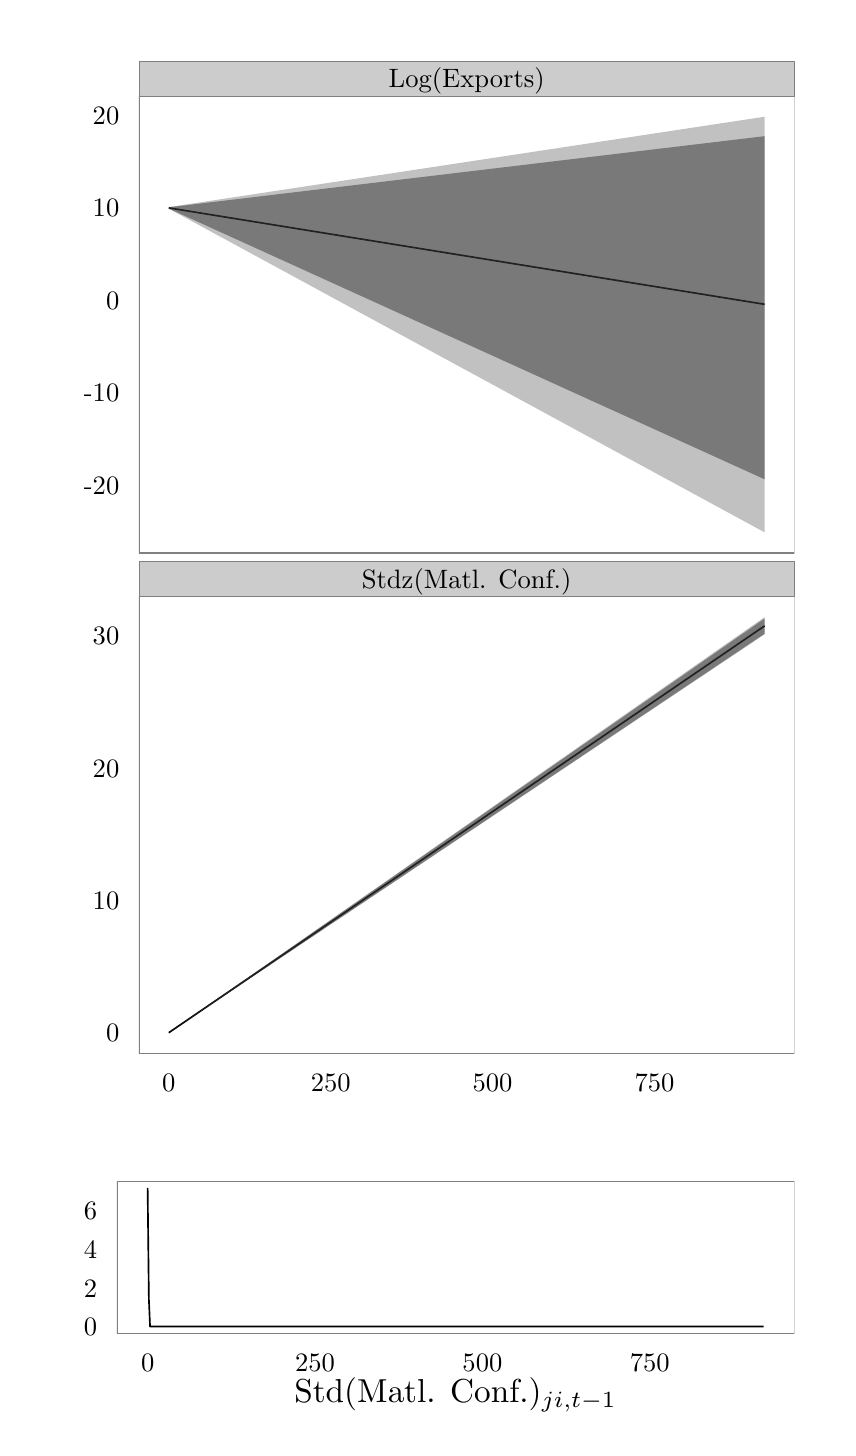
\begin{tikzpicture}[x=1pt,y=1pt]
\definecolor[named]{fillColor}{rgb}{1.00,1.00,1.00}
\path[use as bounding box,fill=fillColor,fill opacity=0.00] (0,0) rectangle (289.08,505.89);
\begin{scope}
\path[clip] (  0.00,101.18) rectangle (289.08,505.89);
\definecolor[named]{drawColor}{rgb}{1.00,1.00,1.00}
\definecolor[named]{fillColor}{rgb}{1.00,1.00,1.00}

\path[draw=drawColor,line width= 0.6pt,line join=round,line cap=round,fill=fillColor] (  0.00,101.18) rectangle (289.08,505.89);
\end{scope}
\begin{scope}
\path[clip] ( 40.22,316.03) rectangle (277.03,481.21);
\definecolor[named]{fillColor}{rgb}{1.00,1.00,1.00}

\path[fill=fillColor] ( 40.22,316.03) rectangle (277.03,481.21);
\definecolor[named]{drawColor}{rgb}{0.00,0.00,0.00}

\path[draw=drawColor,line width= 0.6pt,line join=round] ( 50.98,440.76) --
	(266.27,405.93);
\definecolor[named]{fillColor}{rgb}{0.20,0.20,0.20}

\path[fill=fillColor,fill opacity=0.30] ( 50.98,441.04) --
	(266.27,473.70) --
	(266.27,323.54) --
	( 50.98,440.49) --
	cycle;
\definecolor[named]{fillColor}{rgb}{0.20,0.20,0.20}

\path[fill=fillColor,fill opacity=0.50] ( 50.98,440.98) --
	(266.27,466.68) --
	(266.27,342.70) --
	( 50.98,440.52) --
	cycle;
\definecolor[named]{drawColor}{rgb}{0.50,0.50,0.50}

\path[draw=drawColor,line width= 0.6pt,line join=round,line cap=round] ( 40.22,316.03) rectangle (277.03,481.21);
\end{scope}
\begin{scope}
\path[clip] ( 40.22,135.21) rectangle (277.03,300.39);
\definecolor[named]{fillColor}{rgb}{1.00,1.00,1.00}

\path[fill=fillColor] ( 40.22,135.21) rectangle (277.03,300.39);
\definecolor[named]{drawColor}{rgb}{0.00,0.00,0.00}

\path[draw=drawColor,line width= 0.6pt,line join=round] ( 50.98,142.72) --
	(266.27,289.71);
\definecolor[named]{fillColor}{rgb}{0.20,0.20,0.20}

\path[fill=fillColor,fill opacity=0.30] ( 50.98,142.72) --
	(266.27,292.88) --
	(266.27,286.66) --
	( 50.98,142.72) --
	cycle;
\definecolor[named]{fillColor}{rgb}{0.20,0.20,0.20}

\path[fill=fillColor,fill opacity=0.50] ( 50.98,142.72) --
	(266.27,292.37) --
	(266.27,286.89) --
	( 50.98,142.72) --
	cycle;
\definecolor[named]{drawColor}{rgb}{0.50,0.50,0.50}

\path[draw=drawColor,line width= 0.6pt,line join=round,line cap=round] ( 40.22,135.21) rectangle (277.03,300.39);
\end{scope}
\begin{scope}
\path[clip] (  0.00,  0.00) rectangle (289.08,505.89);
\definecolor[named]{drawColor}{rgb}{0.50,0.50,0.50}
\definecolor[named]{fillColor}{rgb}{0.80,0.80,0.80}

\path[draw=drawColor,line width= 0.2pt,line join=round,line cap=round,fill=fillColor] ( 40.22,481.21) rectangle (277.03,493.84);
\definecolor[named]{drawColor}{rgb}{0.00,0.00,0.00}

\node[text=drawColor,anchor=base,inner sep=0pt, outer sep=0pt, scale=  0.96] at (158.63,484.22) {Log(Exports)};
\end{scope}
\begin{scope}
\path[clip] (  0.00,  0.00) rectangle (289.08,505.89);
\definecolor[named]{drawColor}{rgb}{0.50,0.50,0.50}
\definecolor[named]{fillColor}{rgb}{0.80,0.80,0.80}

\path[draw=drawColor,line width= 0.2pt,line join=round,line cap=round,fill=fillColor] ( 40.22,300.39) rectangle (277.03,313.02);
\definecolor[named]{drawColor}{rgb}{0.00,0.00,0.00}

\node[text=drawColor,anchor=base,inner sep=0pt, outer sep=0pt, scale=  0.96] at (158.63,303.40) {Stdz(Matl. Conf.)};
\end{scope}
\begin{scope}
\path[clip] (  0.00,  0.00) rectangle (289.08,505.89);
\definecolor[named]{drawColor}{rgb}{0.00,0.00,0.00}

\node[text=drawColor,anchor=base east,inner sep=0pt, outer sep=0pt, scale=  0.96] at ( 33.11,337.29) {-20};

\node[text=drawColor,anchor=base east,inner sep=0pt, outer sep=0pt, scale=  0.96] at ( 33.11,370.72) {-10};

\node[text=drawColor,anchor=base east,inner sep=0pt, outer sep=0pt, scale=  0.96] at ( 33.11,404.15) {0};

\node[text=drawColor,anchor=base east,inner sep=0pt, outer sep=0pt, scale=  0.96] at ( 33.11,437.58) {10};

\node[text=drawColor,anchor=base east,inner sep=0pt, outer sep=0pt, scale=  0.96] at ( 33.11,471.01) {20};
\end{scope}
\begin{scope}
\path[clip] (  0.00,  0.00) rectangle (289.08,505.89);
\definecolor[named]{drawColor}{rgb}{0.00,0.00,0.00}

\node[text=drawColor,anchor=base east,inner sep=0pt, outer sep=0pt, scale=  0.96] at ( 33.11,139.48) {0};

\node[text=drawColor,anchor=base east,inner sep=0pt, outer sep=0pt, scale=  0.96] at ( 33.11,187.27) {10};

\node[text=drawColor,anchor=base east,inner sep=0pt, outer sep=0pt, scale=  0.96] at ( 33.11,235.06) {20};

\node[text=drawColor,anchor=base east,inner sep=0pt, outer sep=0pt, scale=  0.96] at ( 33.11,282.86) {30};
\end{scope}
\begin{scope}
\path[clip] (  0.00,  0.00) rectangle (289.08,505.89);
\definecolor[named]{drawColor}{rgb}{0.00,0.00,0.00}

\node[text=drawColor,anchor=base,inner sep=0pt, outer sep=0pt, scale=  0.96] at ( 50.99,121.49) {0};

\node[text=drawColor,anchor=base,inner sep=0pt, outer sep=0pt, scale=  0.96] at (109.49,121.49) {250};

\node[text=drawColor,anchor=base,inner sep=0pt, outer sep=0pt, scale=  0.96] at (168.00,121.49) {500};

\node[text=drawColor,anchor=base,inner sep=0pt, outer sep=0pt, scale=  0.96] at (226.51,121.49) {750};
\end{scope}
\begin{scope}
\path[clip] (  0.00,  0.00) rectangle (289.08,101.18);
\definecolor[named]{drawColor}{rgb}{1.00,1.00,1.00}
\definecolor[named]{fillColor}{rgb}{1.00,1.00,1.00}

\path[draw=drawColor,line width= 0.6pt,line join=round,line cap=round,fill=fillColor] (  0.00,  0.00) rectangle (289.08,101.18);
\end{scope}
\begin{scope}
\path[clip] ( 32.22, 34.03) rectangle (277.04, 89.13);
\definecolor[named]{fillColor}{rgb}{1.00,1.00,1.00}

\path[fill=fillColor] ( 32.22, 34.03) rectangle (277.03, 89.13);
\definecolor[named]{drawColor}{rgb}{0.00,0.00,0.00}

\path[draw=drawColor,line width= 0.6pt,line join=round] ( 43.35, 86.63) --
	( 43.79, 46.61) --
	( 44.22, 36.58) --
	( 44.66, 36.55) --
	( 45.09, 36.55) --
	( 45.53, 36.54) --
	( 45.96, 36.54) --
	( 46.40, 36.54) --
	( 46.83, 36.54) --
	( 47.27, 36.54) --
	( 47.70, 36.54) --
	( 48.14, 36.54) --
	( 48.58, 36.54) --
	( 49.01, 36.54) --
	( 49.45, 36.54) --
	( 49.88, 36.54) --
	( 50.32, 36.54) --
	( 50.75, 36.54) --
	( 51.19, 36.54) --
	( 51.62, 36.54) --
	( 52.06, 36.54) --
	( 52.50, 36.54) --
	( 52.93, 36.54) --
	( 53.37, 36.54) --
	( 53.80, 36.54) --
	( 54.24, 36.54) --
	( 54.67, 36.54) --
	( 55.11, 36.54) --
	( 55.54, 36.54) --
	( 55.98, 36.54) --
	( 56.42, 36.54) --
	( 56.85, 36.54) --
	( 57.29, 36.54) --
	( 57.72, 36.54) --
	( 58.16, 36.54) --
	( 58.59, 36.54) --
	( 59.03, 36.54) --
	( 59.46, 36.54) --
	( 59.90, 36.54) --
	( 60.34, 36.54) --
	( 60.77, 36.54) --
	( 61.21, 36.54) --
	( 61.64, 36.54) --
	( 62.08, 36.54) --
	( 62.51, 36.54) --
	( 62.95, 36.54) --
	( 63.38, 36.54) --
	( 63.82, 36.54) --
	( 64.26, 36.54) --
	( 64.69, 36.54) --
	( 65.13, 36.54) --
	( 65.56, 36.54) --
	( 66.00, 36.54) --
	( 66.43, 36.54) --
	( 66.87, 36.54) --
	( 67.30, 36.54) --
	( 67.74, 36.54) --
	( 68.17, 36.54) --
	( 68.61, 36.54) --
	( 69.05, 36.54) --
	( 69.48, 36.54) --
	( 69.92, 36.54) --
	( 70.35, 36.54) --
	( 70.79, 36.54) --
	( 71.22, 36.54) --
	( 71.66, 36.54) --
	( 72.09, 36.54) --
	( 72.53, 36.54) --
	( 72.97, 36.54) --
	( 73.40, 36.54) --
	( 73.84, 36.54) --
	( 74.27, 36.54) --
	( 74.71, 36.54) --
	( 75.14, 36.54) --
	( 75.58, 36.54) --
	( 76.01, 36.54) --
	( 76.45, 36.54) --
	( 76.89, 36.54) --
	( 77.32, 36.54) --
	( 77.76, 36.54) --
	( 78.19, 36.54) --
	( 78.63, 36.54) --
	( 79.06, 36.54) --
	( 79.50, 36.54) --
	( 79.93, 36.54) --
	( 80.37, 36.54) --
	( 80.81, 36.54) --
	( 81.24, 36.54) --
	( 81.68, 36.54) --
	( 82.11, 36.54) --
	( 82.55, 36.54) --
	( 82.98, 36.54) --
	( 83.42, 36.54) --
	( 83.85, 36.54) --
	( 84.29, 36.54) --
	( 84.73, 36.54) --
	( 85.16, 36.54) --
	( 85.60, 36.54) --
	( 86.03, 36.54) --
	( 86.47, 36.54) --
	( 86.90, 36.54) --
	( 87.34, 36.54) --
	( 87.77, 36.54) --
	( 88.21, 36.54) --
	( 88.65, 36.54) --
	( 89.08, 36.54) --
	( 89.52, 36.54) --
	( 89.95, 36.54) --
	( 90.39, 36.54) --
	( 90.82, 36.54) --
	( 91.26, 36.54) --
	( 91.69, 36.54) --
	( 92.13, 36.54) --
	( 92.56, 36.54) --
	( 93.00, 36.54) --
	( 93.44, 36.54) --
	( 93.87, 36.54) --
	( 94.31, 36.54) --
	( 94.74, 36.54) --
	( 95.18, 36.54) --
	( 95.61, 36.54) --
	( 96.05, 36.54) --
	( 96.48, 36.54) --
	( 96.92, 36.54) --
	( 97.36, 36.54) --
	( 97.79, 36.54) --
	( 98.23, 36.54) --
	( 98.66, 36.54) --
	( 99.10, 36.54) --
	( 99.53, 36.54) --
	( 99.97, 36.54) --
	(100.40, 36.54) --
	(100.84, 36.54) --
	(101.28, 36.54) --
	(101.71, 36.54) --
	(102.15, 36.54) --
	(102.58, 36.54) --
	(103.02, 36.54) --
	(103.45, 36.54) --
	(103.89, 36.54) --
	(104.32, 36.54) --
	(104.76, 36.54) --
	(105.20, 36.54) --
	(105.63, 36.54) --
	(106.07, 36.54) --
	(106.50, 36.54) --
	(106.94, 36.54) --
	(107.37, 36.54) --
	(107.81, 36.54) --
	(108.24, 36.54) --
	(108.68, 36.54) --
	(109.12, 36.54) --
	(109.55, 36.54) --
	(109.99, 36.54) --
	(110.42, 36.54) --
	(110.86, 36.54) --
	(111.29, 36.54) --
	(111.73, 36.54) --
	(112.16, 36.54) --
	(112.60, 36.54) --
	(113.03, 36.54) --
	(113.47, 36.54) --
	(113.91, 36.54) --
	(114.34, 36.54) --
	(114.78, 36.54) --
	(115.21, 36.54) --
	(115.65, 36.54) --
	(116.08, 36.54) --
	(116.52, 36.54) --
	(116.95, 36.54) --
	(117.39, 36.54) --
	(117.83, 36.54) --
	(118.26, 36.54) --
	(118.70, 36.54) --
	(119.13, 36.54) --
	(119.57, 36.54) --
	(120.00, 36.54) --
	(120.44, 36.54) --
	(120.87, 36.54) --
	(121.31, 36.54) --
	(121.75, 36.54) --
	(122.18, 36.54) --
	(122.62, 36.54) --
	(123.05, 36.54) --
	(123.49, 36.54) --
	(123.92, 36.54) --
	(124.36, 36.54) --
	(124.79, 36.54) --
	(125.23, 36.54) --
	(125.67, 36.54) --
	(126.10, 36.54) --
	(126.54, 36.54) --
	(126.97, 36.54) --
	(127.41, 36.54) --
	(127.84, 36.54) --
	(128.28, 36.54) --
	(128.71, 36.54) --
	(129.15, 36.54) --
	(129.59, 36.54) --
	(130.02, 36.54) --
	(130.46, 36.54) --
	(130.89, 36.54) --
	(131.33, 36.54) --
	(131.76, 36.54) --
	(132.20, 36.54) --
	(132.63, 36.54) --
	(133.07, 36.54) --
	(133.50, 36.54) --
	(133.94, 36.54) --
	(134.38, 36.54) --
	(134.81, 36.54) --
	(135.25, 36.54) --
	(135.68, 36.54) --
	(136.12, 36.54) --
	(136.55, 36.54) --
	(136.99, 36.54) --
	(137.42, 36.54) --
	(137.86, 36.54) --
	(138.30, 36.54) --
	(138.73, 36.54) --
	(139.17, 36.54) --
	(139.60, 36.54) --
	(140.04, 36.54) --
	(140.47, 36.54) --
	(140.91, 36.54) --
	(141.34, 36.54) --
	(141.78, 36.54) --
	(142.22, 36.54) --
	(142.65, 36.54) --
	(143.09, 36.54) --
	(143.52, 36.54) --
	(143.96, 36.54) --
	(144.39, 36.54) --
	(144.83, 36.54) --
	(145.26, 36.54) --
	(145.70, 36.54) --
	(146.14, 36.54) --
	(146.57, 36.54) --
	(147.01, 36.54) --
	(147.44, 36.54) --
	(147.88, 36.54) --
	(148.31, 36.54) --
	(148.75, 36.54) --
	(149.18, 36.54) --
	(149.62, 36.54) --
	(150.06, 36.54) --
	(150.49, 36.54) --
	(150.93, 36.54) --
	(151.36, 36.54) --
	(151.80, 36.54) --
	(152.23, 36.54) --
	(152.67, 36.54) --
	(153.10, 36.54) --
	(153.54, 36.54) --
	(153.98, 36.54) --
	(154.41, 36.54) --
	(154.85, 36.54) --
	(155.28, 36.54) --
	(155.72, 36.54) --
	(156.15, 36.54) --
	(156.59, 36.54) --
	(157.02, 36.54) --
	(157.46, 36.54) --
	(157.89, 36.54) --
	(158.33, 36.54) --
	(158.77, 36.54) --
	(159.20, 36.54) --
	(159.64, 36.54) --
	(160.07, 36.54) --
	(160.51, 36.54) --
	(160.94, 36.54) --
	(161.38, 36.54) --
	(161.81, 36.54) --
	(162.25, 36.54) --
	(162.69, 36.54) --
	(163.12, 36.54) --
	(163.56, 36.54) --
	(163.99, 36.54) --
	(164.43, 36.54) --
	(164.86, 36.54) --
	(165.30, 36.54) --
	(165.73, 36.54) --
	(166.17, 36.54) --
	(166.61, 36.54) --
	(167.04, 36.54) --
	(167.48, 36.54) --
	(167.91, 36.54) --
	(168.35, 36.54) --
	(168.78, 36.54) --
	(169.22, 36.54) --
	(169.65, 36.54) --
	(170.09, 36.54) --
	(170.53, 36.54) --
	(170.96, 36.54) --
	(171.40, 36.54) --
	(171.83, 36.54) --
	(172.27, 36.54) --
	(172.70, 36.54) --
	(173.14, 36.54) --
	(173.57, 36.54) --
	(174.01, 36.54) --
	(174.45, 36.54) --
	(174.88, 36.54) --
	(175.32, 36.54) --
	(175.75, 36.54) --
	(176.19, 36.54) --
	(176.62, 36.54) --
	(177.06, 36.54) --
	(177.49, 36.54) --
	(177.93, 36.54) --
	(178.36, 36.54) --
	(178.80, 36.54) --
	(179.24, 36.54) --
	(179.67, 36.54) --
	(180.11, 36.54) --
	(180.54, 36.54) --
	(180.98, 36.54) --
	(181.41, 36.54) --
	(181.85, 36.54) --
	(182.28, 36.54) --
	(182.72, 36.54) --
	(183.16, 36.54) --
	(183.59, 36.54) --
	(184.03, 36.54) --
	(184.46, 36.54) --
	(184.90, 36.54) --
	(185.33, 36.54) --
	(185.77, 36.54) --
	(186.20, 36.54) --
	(186.64, 36.54) --
	(187.08, 36.54) --
	(187.51, 36.54) --
	(187.95, 36.54) --
	(188.38, 36.54) --
	(188.82, 36.54) --
	(189.25, 36.54) --
	(189.69, 36.54) --
	(190.12, 36.54) --
	(190.56, 36.54) --
	(191.00, 36.54) --
	(191.43, 36.54) --
	(191.87, 36.54) --
	(192.30, 36.54) --
	(192.74, 36.54) --
	(193.17, 36.54) --
	(193.61, 36.54) --
	(194.04, 36.54) --
	(194.48, 36.54) --
	(194.92, 36.54) --
	(195.35, 36.54) --
	(195.79, 36.54) --
	(196.22, 36.54) --
	(196.66, 36.54) --
	(197.09, 36.54) --
	(197.53, 36.54) --
	(197.96, 36.54) --
	(198.40, 36.54) --
	(198.83, 36.54) --
	(199.27, 36.54) --
	(199.71, 36.54) --
	(200.14, 36.54) --
	(200.58, 36.54) --
	(201.01, 36.54) --
	(201.45, 36.54) --
	(201.88, 36.54) --
	(202.32, 36.54) --
	(202.75, 36.54) --
	(203.19, 36.54) --
	(203.63, 36.54) --
	(204.06, 36.54) --
	(204.50, 36.54) --
	(204.93, 36.54) --
	(205.37, 36.54) --
	(205.80, 36.54) --
	(206.24, 36.54) --
	(206.67, 36.54) --
	(207.11, 36.54) --
	(207.55, 36.54) --
	(207.98, 36.54) --
	(208.42, 36.54) --
	(208.85, 36.54) --
	(209.29, 36.54) --
	(209.72, 36.54) --
	(210.16, 36.54) --
	(210.59, 36.54) --
	(211.03, 36.54) --
	(211.47, 36.54) --
	(211.90, 36.54) --
	(212.34, 36.54) --
	(212.77, 36.54) --
	(213.21, 36.54) --
	(213.64, 36.54) --
	(214.08, 36.54) --
	(214.51, 36.54) --
	(214.95, 36.54) --
	(215.39, 36.54) --
	(215.82, 36.54) --
	(216.26, 36.54) --
	(216.69, 36.54) --
	(217.13, 36.54) --
	(217.56, 36.54) --
	(218.00, 36.54) --
	(218.43, 36.54) --
	(218.87, 36.54) --
	(219.31, 36.54) --
	(219.74, 36.54) --
	(220.18, 36.54) --
	(220.61, 36.54) --
	(221.05, 36.54) --
	(221.48, 36.54) --
	(221.92, 36.54) --
	(222.35, 36.54) --
	(222.79, 36.54) --
	(223.22, 36.54) --
	(223.66, 36.54) --
	(224.10, 36.54) --
	(224.53, 36.54) --
	(224.97, 36.54) --
	(225.40, 36.54) --
	(225.84, 36.54) --
	(226.27, 36.54) --
	(226.71, 36.54) --
	(227.14, 36.54) --
	(227.58, 36.54) --
	(228.02, 36.54) --
	(228.45, 36.54) --
	(228.89, 36.54) --
	(229.32, 36.54) --
	(229.76, 36.54) --
	(230.19, 36.54) --
	(230.63, 36.54) --
	(231.06, 36.54) --
	(231.50, 36.54) --
	(231.94, 36.54) --
	(232.37, 36.54) --
	(232.81, 36.54) --
	(233.24, 36.54) --
	(233.68, 36.54) --
	(234.11, 36.54) --
	(234.55, 36.54) --
	(234.98, 36.54) --
	(235.42, 36.54) --
	(235.86, 36.54) --
	(236.29, 36.54) --
	(236.73, 36.54) --
	(237.16, 36.54) --
	(237.60, 36.54) --
	(238.03, 36.54) --
	(238.47, 36.54) --
	(238.90, 36.54) --
	(239.34, 36.54) --
	(239.78, 36.54) --
	(240.21, 36.54) --
	(240.65, 36.54) --
	(241.08, 36.54) --
	(241.52, 36.54) --
	(241.95, 36.54) --
	(242.39, 36.54) --
	(242.82, 36.54) --
	(243.26, 36.54) --
	(243.69, 36.54) --
	(244.13, 36.54) --
	(244.57, 36.54) --
	(245.00, 36.54) --
	(245.44, 36.54) --
	(245.87, 36.54) --
	(246.31, 36.54) --
	(246.74, 36.54) --
	(247.18, 36.54) --
	(247.61, 36.54) --
	(248.05, 36.54) --
	(248.49, 36.54) --
	(248.92, 36.54) --
	(249.36, 36.54) --
	(249.79, 36.54) --
	(250.23, 36.54) --
	(250.66, 36.54) --
	(251.10, 36.54) --
	(251.53, 36.54) --
	(251.97, 36.54) --
	(252.41, 36.54) --
	(252.84, 36.54) --
	(253.28, 36.54) --
	(253.71, 36.54) --
	(254.15, 36.54) --
	(254.58, 36.54) --
	(255.02, 36.54) --
	(255.45, 36.54) --
	(255.89, 36.54) --
	(256.33, 36.54) --
	(256.76, 36.54) --
	(257.20, 36.54) --
	(257.63, 36.54) --
	(258.07, 36.54) --
	(258.50, 36.54) --
	(258.94, 36.54) --
	(259.37, 36.54) --
	(259.81, 36.54) --
	(260.25, 36.54) --
	(260.68, 36.54) --
	(261.12, 36.54) --
	(261.55, 36.54) --
	(261.99, 36.54) --
	(262.42, 36.54) --
	(262.86, 36.54) --
	(263.29, 36.54) --
	(263.73, 36.54) --
	(264.16, 36.54) --
	(264.60, 36.54) --
	(265.04, 36.54) --
	(265.47, 36.54) --
	(265.91, 36.54);
\definecolor[named]{drawColor}{rgb}{0.50,0.50,0.50}

\path[draw=drawColor,line width= 0.6pt,line join=round,line cap=round] ( 32.22, 34.03) rectangle (277.03, 89.13);
\end{scope}
\begin{scope}
\path[clip] (  0.00,  0.00) rectangle (289.08,505.89);
\definecolor[named]{drawColor}{rgb}{0.00,0.00,0.00}

\node[text=drawColor,anchor=base east,inner sep=0pt, outer sep=0pt, scale=  0.96] at ( 25.11, 33.23) {0};

\node[text=drawColor,anchor=base east,inner sep=0pt, outer sep=0pt, scale=  0.96] at ( 25.11, 47.18) {2};

\node[text=drawColor,anchor=base east,inner sep=0pt, outer sep=0pt, scale=  0.96] at ( 25.11, 61.12) {4};

\node[text=drawColor,anchor=base east,inner sep=0pt, outer sep=0pt, scale=  0.96] at ( 25.11, 75.06) {6};
\end{scope}
\begin{scope}
\path[clip] (  0.00,  0.00) rectangle (289.08,505.89);
\definecolor[named]{drawColor}{rgb}{0.00,0.00,0.00}

\node[text=drawColor,anchor=base,inner sep=0pt, outer sep=0pt, scale=  0.96] at ( 43.39, 20.31) {0};

\node[text=drawColor,anchor=base,inner sep=0pt, outer sep=0pt, scale=  0.96] at (103.85, 20.31) {250};

\node[text=drawColor,anchor=base,inner sep=0pt, outer sep=0pt, scale=  0.96] at (164.32, 20.31) {500};

\node[text=drawColor,anchor=base,inner sep=0pt, outer sep=0pt, scale=  0.96] at (224.78, 20.31) {750};
\end{scope}
\begin{scope}
\path[clip] (  0.00,  0.00) rectangle (289.08,505.89);
\definecolor[named]{drawColor}{rgb}{0.00,0.00,0.00}

\node[text=drawColor,anchor=base,inner sep=0pt, outer sep=0pt, scale=  1.20] at (154.63,  9.03) {Std(Matl. Conf.)$_{ji, t-1}$};
\end{scope}
\end{tikzpicture}
}  &
      \resizebox{.38\textwidth}{!}{% Created by tikzDevice version 0.7.0 on 2015-07-01 08:54:08
% !TEX encoding = UTF-8 Unicode
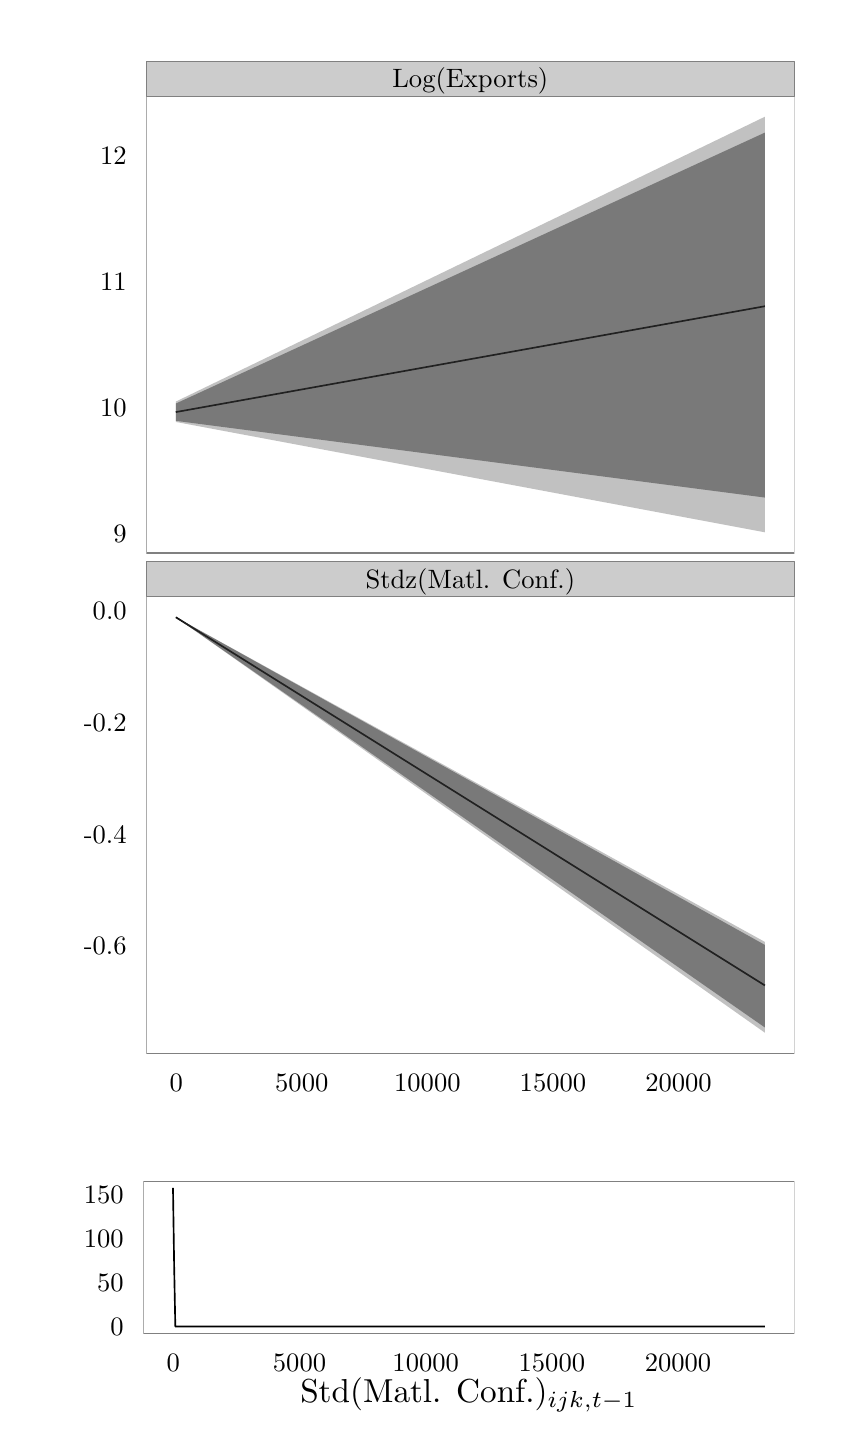
\begin{tikzpicture}[x=1pt,y=1pt]
\definecolor[named]{fillColor}{rgb}{1.00,1.00,1.00}
\path[use as bounding box,fill=fillColor,fill opacity=0.00] (0,0) rectangle (289.08,505.89);
\begin{scope}
\path[clip] (  0.00,101.18) rectangle (289.08,505.89);
\definecolor[named]{drawColor}{rgb}{1.00,1.00,1.00}
\definecolor[named]{fillColor}{rgb}{1.00,1.00,1.00}

\path[draw=drawColor,line width= 0.6pt,line join=round,line cap=round,fill=fillColor] ( -0.00,101.18) rectangle (289.08,505.89);
\end{scope}
\begin{scope}
\path[clip] ( 42.89,316.03) rectangle (277.04,481.21);
\definecolor[named]{fillColor}{rgb}{1.00,1.00,1.00}

\path[fill=fillColor] ( 42.89,316.03) rectangle (277.03,481.21);
\definecolor[named]{drawColor}{rgb}{0.00,0.00,0.00}

\path[draw=drawColor,line width= 0.6pt,line join=round] ( 53.53,366.98) --
	( 53.65,367.00) --
	( 53.65,367.00) --
	( 53.65,367.00) --
	( 53.65,367.00) --
	( 53.65,367.00) --
	( 53.65,367.00) --
	( 53.65,367.00) --
	( 53.65,367.00) --
	( 53.65,367.00) --
	( 53.65,367.00) --
	( 53.65,367.00) --
	( 53.65,367.00) --
	( 53.65,367.00) --
	( 53.65,367.00) --
	( 53.65,367.00) --
	( 53.65,367.00) --
	( 53.65,367.00) --
	( 53.65,367.00) --
	( 53.66,367.00) --
	(266.39,405.23);
\definecolor[named]{fillColor}{rgb}{0.20,0.20,0.20}

\path[fill=fillColor,fill opacity=0.30] ( 53.53,370.82) --
	( 53.65,370.84) --
	( 53.65,370.84) --
	( 53.65,370.84) --
	( 53.65,370.84) --
	( 53.65,370.84) --
	( 53.65,370.84) --
	( 53.65,370.84) --
	( 53.65,370.84) --
	( 53.65,370.84) --
	( 53.65,370.84) --
	( 53.65,370.84) --
	( 53.65,370.84) --
	( 53.65,370.84) --
	( 53.65,370.84) --
	( 53.65,370.84) --
	( 53.65,370.84) --
	( 53.65,370.84) --
	( 53.65,370.84) --
	( 53.66,370.84) --
	(266.39,473.70) --
	(266.39,323.54) --
	( 53.66,363.39) --
	( 53.65,363.39) --
	( 53.65,363.39) --
	( 53.65,363.39) --
	( 53.65,363.39) --
	( 53.65,363.39) --
	( 53.65,363.39) --
	( 53.65,363.39) --
	( 53.65,363.39) --
	( 53.65,363.39) --
	( 53.65,363.39) --
	( 53.65,363.39) --
	( 53.65,363.39) --
	( 53.65,363.39) --
	( 53.65,363.39) --
	( 53.65,363.39) --
	( 53.65,363.39) --
	( 53.65,363.39) --
	( 53.65,363.39) --
	( 53.53,363.36) --
	cycle;
\definecolor[named]{fillColor}{rgb}{0.20,0.20,0.20}

\path[fill=fillColor,fill opacity=0.50] ( 53.53,370.11) --
	( 53.65,370.12) --
	( 53.65,370.12) --
	( 53.65,370.12) --
	( 53.65,370.12) --
	( 53.65,370.12) --
	( 53.65,370.12) --
	( 53.65,370.12) --
	( 53.65,370.12) --
	( 53.65,370.12) --
	( 53.65,370.12) --
	( 53.65,370.12) --
	( 53.65,370.12) --
	( 53.65,370.12) --
	( 53.65,370.12) --
	( 53.65,370.12) --
	( 53.65,370.12) --
	( 53.65,370.12) --
	( 53.65,370.12) --
	( 53.66,370.12) --
	(266.39,467.97) --
	(266.39,336.09) --
	( 53.66,363.80) --
	( 53.65,363.80) --
	( 53.65,363.80) --
	( 53.65,363.80) --
	( 53.65,363.80) --
	( 53.65,363.80) --
	( 53.65,363.80) --
	( 53.65,363.80) --
	( 53.65,363.80) --
	( 53.65,363.80) --
	( 53.65,363.80) --
	( 53.65,363.80) --
	( 53.65,363.80) --
	( 53.65,363.80) --
	( 53.65,363.80) --
	( 53.65,363.80) --
	( 53.65,363.80) --
	( 53.65,363.80) --
	( 53.65,363.80) --
	( 53.53,363.79) --
	cycle;
\definecolor[named]{drawColor}{rgb}{0.50,0.50,0.50}

\path[draw=drawColor,line width= 0.6pt,line join=round,line cap=round] ( 42.89,316.03) rectangle (277.03,481.21);
\end{scope}
\begin{scope}
\path[clip] ( 42.89,135.21) rectangle (277.04,300.39);
\definecolor[named]{fillColor}{rgb}{1.00,1.00,1.00}

\path[fill=fillColor] ( 42.89,135.21) rectangle (277.03,300.39);
\definecolor[named]{drawColor}{rgb}{0.00,0.00,0.00}

\path[draw=drawColor,line width= 0.6pt,line join=round] ( 53.53,292.85) --
	( 53.65,292.78) --
	( 53.65,292.78) --
	( 53.65,292.78) --
	( 53.65,292.78) --
	( 53.65,292.78) --
	( 53.65,292.78) --
	( 53.65,292.78) --
	( 53.65,292.78) --
	( 53.65,292.78) --
	( 53.65,292.78) --
	( 53.65,292.78) --
	( 53.65,292.78) --
	( 53.65,292.78) --
	( 53.65,292.78) --
	( 53.65,292.78) --
	( 53.65,292.78) --
	( 53.65,292.78) --
	( 53.65,292.78) --
	( 53.66,292.77) --
	(266.39,159.80);
\definecolor[named]{fillColor}{rgb}{0.20,0.20,0.20}

\path[fill=fillColor,fill opacity=0.30] ( 53.53,292.88) --
	( 53.65,292.81) --
	( 53.65,292.81) --
	( 53.65,292.80) --
	( 53.65,292.80) --
	( 53.65,292.80) --
	( 53.65,292.80) --
	( 53.65,292.80) --
	( 53.65,292.80) --
	( 53.65,292.80) --
	( 53.65,292.80) --
	( 53.65,292.80) --
	( 53.65,292.80) --
	( 53.65,292.80) --
	( 53.65,292.80) --
	( 53.65,292.80) --
	( 53.65,292.80) --
	( 53.65,292.80) --
	( 53.65,292.80) --
	( 53.66,292.80) --
	(266.39,175.53) --
	(266.39,142.72) --
	( 53.66,292.75) --
	( 53.65,292.75) --
	( 53.65,292.75) --
	( 53.65,292.75) --
	( 53.65,292.75) --
	( 53.65,292.75) --
	( 53.65,292.75) --
	( 53.65,292.75) --
	( 53.65,292.75) --
	( 53.65,292.75) --
	( 53.65,292.75) --
	( 53.65,292.75) --
	( 53.65,292.75) --
	( 53.65,292.75) --
	( 53.65,292.75) --
	( 53.65,292.75) --
	( 53.65,292.75) --
	( 53.65,292.75) --
	( 53.65,292.75) --
	( 53.53,292.83) --
	cycle;
\definecolor[named]{fillColor}{rgb}{0.20,0.20,0.20}

\path[fill=fillColor,fill opacity=0.50] ( 53.53,292.88) --
	( 53.65,292.80) --
	( 53.65,292.80) --
	( 53.65,292.80) --
	( 53.65,292.80) --
	( 53.65,292.80) --
	( 53.65,292.80) --
	( 53.65,292.80) --
	( 53.65,292.80) --
	( 53.65,292.80) --
	( 53.65,292.80) --
	( 53.65,292.80) --
	( 53.65,292.80) --
	( 53.65,292.80) --
	( 53.65,292.80) --
	( 53.65,292.80) --
	( 53.65,292.80) --
	( 53.65,292.80) --
	( 53.65,292.80) --
	( 53.66,292.80) --
	(266.39,174.44) --
	(266.39,144.61) --
	( 53.66,292.75) --
	( 53.65,292.75) --
	( 53.65,292.75) --
	( 53.65,292.75) --
	( 53.65,292.75) --
	( 53.65,292.75) --
	( 53.65,292.75) --
	( 53.65,292.75) --
	( 53.65,292.75) --
	( 53.65,292.75) --
	( 53.65,292.75) --
	( 53.65,292.75) --
	( 53.65,292.75) --
	( 53.65,292.75) --
	( 53.65,292.75) --
	( 53.65,292.75) --
	( 53.65,292.75) --
	( 53.65,292.75) --
	( 53.65,292.75) --
	( 53.53,292.83) --
	cycle;
\definecolor[named]{drawColor}{rgb}{0.50,0.50,0.50}

\path[draw=drawColor,line width= 0.6pt,line join=round,line cap=round] ( 42.89,135.21) rectangle (277.03,300.39);
\end{scope}
\begin{scope}
\path[clip] (  0.00,  0.00) rectangle (289.08,505.89);
\definecolor[named]{drawColor}{rgb}{0.50,0.50,0.50}
\definecolor[named]{fillColor}{rgb}{0.80,0.80,0.80}

\path[draw=drawColor,line width= 0.2pt,line join=round,line cap=round,fill=fillColor] ( 42.89,481.21) rectangle (277.03,493.84);
\definecolor[named]{drawColor}{rgb}{0.00,0.00,0.00}

\node[text=drawColor,anchor=base,inner sep=0pt, outer sep=0pt, scale=  0.96] at (159.96,484.22) {Log(Exports)};
\end{scope}
\begin{scope}
\path[clip] (  0.00,  0.00) rectangle (289.08,505.89);
\definecolor[named]{drawColor}{rgb}{0.50,0.50,0.50}
\definecolor[named]{fillColor}{rgb}{0.80,0.80,0.80}

\path[draw=drawColor,line width= 0.2pt,line join=round,line cap=round,fill=fillColor] ( 42.89,300.39) rectangle (277.03,313.02);
\definecolor[named]{drawColor}{rgb}{0.00,0.00,0.00}

\node[text=drawColor,anchor=base,inner sep=0pt, outer sep=0pt, scale=  0.96] at (159.96,303.40) {Stdz(Matl. Conf.)};
\end{scope}
\begin{scope}
\path[clip] (  0.00,  0.00) rectangle (289.08,505.89);
\definecolor[named]{drawColor}{rgb}{0.00,0.00,0.00}

\node[text=drawColor,anchor=base east,inner sep=0pt, outer sep=0pt, scale=  0.96] at ( 35.77,320.03) {9};

\node[text=drawColor,anchor=base east,inner sep=0pt, outer sep=0pt, scale=  0.96] at ( 35.77,365.49) {10};

\node[text=drawColor,anchor=base east,inner sep=0pt, outer sep=0pt, scale=  0.96] at ( 35.77,410.96) {11};

\node[text=drawColor,anchor=base east,inner sep=0pt, outer sep=0pt, scale=  0.96] at ( 35.77,456.42) {12};
\end{scope}
\begin{scope}
\path[clip] (  0.00,  0.00) rectangle (289.08,505.89);
\definecolor[named]{drawColor}{rgb}{0.00,0.00,0.00}

\node[text=drawColor,anchor=base east,inner sep=0pt, outer sep=0pt, scale=  0.96] at ( 35.77,170.82) {-0.6};

\node[text=drawColor,anchor=base east,inner sep=0pt, outer sep=0pt, scale=  0.96] at ( 35.77,211.27) {-0.4};

\node[text=drawColor,anchor=base east,inner sep=0pt, outer sep=0pt, scale=  0.96] at ( 35.77,251.73) {-0.2};

\node[text=drawColor,anchor=base east,inner sep=0pt, outer sep=0pt, scale=  0.96] at ( 35.77,292.19) {0.0};
\end{scope}
\begin{scope}
\path[clip] (  0.00,  0.00) rectangle (289.08,505.89);
\definecolor[named]{drawColor}{rgb}{0.00,0.00,0.00}

\node[text=drawColor,anchor=base,inner sep=0pt, outer sep=0pt, scale=  0.96] at ( 53.65,121.49) {0};

\node[text=drawColor,anchor=base,inner sep=0pt, outer sep=0pt, scale=  0.96] at ( 99.04,121.49) {5000};

\node[text=drawColor,anchor=base,inner sep=0pt, outer sep=0pt, scale=  0.96] at (144.43,121.49) {10000};

\node[text=drawColor,anchor=base,inner sep=0pt, outer sep=0pt, scale=  0.96] at (189.81,121.49) {15000};

\node[text=drawColor,anchor=base,inner sep=0pt, outer sep=0pt, scale=  0.96] at (235.20,121.49) {20000};
\end{scope}
\begin{scope}
\path[clip] (  0.00,  0.00) rectangle (289.08,101.18);
\definecolor[named]{drawColor}{rgb}{1.00,1.00,1.00}
\definecolor[named]{fillColor}{rgb}{1.00,1.00,1.00}

\path[draw=drawColor,line width= 0.6pt,line join=round,line cap=round,fill=fillColor] ( -0.00,  0.00) rectangle (289.08,101.18);
\end{scope}
\begin{scope}
\path[clip] ( 41.82, 34.03) rectangle (277.04, 89.13);
\definecolor[named]{fillColor}{rgb}{1.00,1.00,1.00}

\path[fill=fillColor] ( 41.82, 34.03) rectangle (277.03, 89.13);
\definecolor[named]{drawColor}{rgb}{0.00,0.00,0.00}

\path[draw=drawColor,line width= 0.6pt,line join=round] ( 52.51, 86.63) --
	( 52.93, 58.38) --
	( 53.35, 36.58) --
	( 53.77, 36.55) --
	( 54.18, 36.55) --
	( 54.60, 36.54) --
	( 55.02, 36.54) --
	( 55.44, 36.54) --
	( 55.86, 36.54) --
	( 56.28, 36.54) --
	( 56.70, 36.54) --
	( 57.11, 36.54) --
	( 57.53, 36.54) --
	( 57.95, 36.54) --
	( 58.37, 36.54) --
	( 58.79, 36.54) --
	( 59.21, 36.54) --
	( 59.62, 36.54) --
	( 60.04, 36.54) --
	( 60.46, 36.54) --
	( 60.88, 36.54) --
	( 61.30, 36.54) --
	( 61.72, 36.54) --
	( 62.14, 36.54) --
	( 62.55, 36.54) --
	( 62.97, 36.54) --
	( 63.39, 36.54) --
	( 63.81, 36.54) --
	( 64.23, 36.54) --
	( 64.65, 36.54) --
	( 65.06, 36.54) --
	( 65.48, 36.54) --
	( 65.90, 36.54) --
	( 66.32, 36.54) --
	( 66.74, 36.54) --
	( 67.16, 36.54) --
	( 67.58, 36.54) --
	( 67.99, 36.54) --
	( 68.41, 36.54) --
	( 68.83, 36.54) --
	( 69.25, 36.54) --
	( 69.67, 36.54) --
	( 70.09, 36.54) --
	( 70.50, 36.54) --
	( 70.92, 36.54) --
	( 71.34, 36.54) --
	( 71.76, 36.54) --
	( 72.18, 36.54) --
	( 72.60, 36.54) --
	( 73.02, 36.54) --
	( 73.43, 36.54) --
	( 73.85, 36.54) --
	( 74.27, 36.54) --
	( 74.69, 36.54) --
	( 75.11, 36.54) --
	( 75.53, 36.54) --
	( 75.94, 36.54) --
	( 76.36, 36.54) --
	( 76.78, 36.54) --
	( 77.20, 36.54) --
	( 77.62, 36.54) --
	( 78.04, 36.54) --
	( 78.46, 36.54) --
	( 78.87, 36.54) --
	( 79.29, 36.54) --
	( 79.71, 36.54) --
	( 80.13, 36.54) --
	( 80.55, 36.54) --
	( 80.97, 36.54) --
	( 81.38, 36.54) --
	( 81.80, 36.54) --
	( 82.22, 36.54) --
	( 82.64, 36.54) --
	( 83.06, 36.54) --
	( 83.48, 36.54) --
	( 83.90, 36.54) --
	( 84.31, 36.54) --
	( 84.73, 36.54) --
	( 85.15, 36.54) --
	( 85.57, 36.54) --
	( 85.99, 36.54) --
	( 86.41, 36.54) --
	( 86.82, 36.54) --
	( 87.24, 36.54) --
	( 87.66, 36.54) --
	( 88.08, 36.54) --
	( 88.50, 36.54) --
	( 88.92, 36.54) --
	( 89.34, 36.54) --
	( 89.75, 36.54) --
	( 90.17, 36.54) --
	( 90.59, 36.54) --
	( 91.01, 36.54) --
	( 91.43, 36.54) --
	( 91.85, 36.54) --
	( 92.26, 36.54) --
	( 92.68, 36.54) --
	( 93.10, 36.54) --
	( 93.52, 36.54) --
	( 93.94, 36.54) --
	( 94.36, 36.54) --
	( 94.78, 36.54) --
	( 95.19, 36.54) --
	( 95.61, 36.54) --
	( 96.03, 36.54) --
	( 96.45, 36.54) --
	( 96.87, 36.54) --
	( 97.29, 36.54) --
	( 97.70, 36.54) --
	( 98.12, 36.54) --
	( 98.54, 36.54) --
	( 98.96, 36.54) --
	( 99.38, 36.54) --
	( 99.80, 36.54) --
	(100.22, 36.54) --
	(100.63, 36.54) --
	(101.05, 36.54) --
	(101.47, 36.54) --
	(101.89, 36.54) --
	(102.31, 36.54) --
	(102.73, 36.54) --
	(103.14, 36.54) --
	(103.56, 36.54) --
	(103.98, 36.54) --
	(104.40, 36.54) --
	(104.82, 36.54) --
	(105.24, 36.54) --
	(105.66, 36.54) --
	(106.07, 36.54) --
	(106.49, 36.54) --
	(106.91, 36.54) --
	(107.33, 36.54) --
	(107.75, 36.54) --
	(108.17, 36.54) --
	(108.58, 36.54) --
	(109.00, 36.54) --
	(109.42, 36.54) --
	(109.84, 36.54) --
	(110.26, 36.54) --
	(110.68, 36.54) --
	(111.10, 36.54) --
	(111.51, 36.54) --
	(111.93, 36.54) --
	(112.35, 36.54) --
	(112.77, 36.54) --
	(113.19, 36.54) --
	(113.61, 36.54) --
	(114.02, 36.54) --
	(114.44, 36.54) --
	(114.86, 36.54) --
	(115.28, 36.54) --
	(115.70, 36.54) --
	(116.12, 36.54) --
	(116.54, 36.54) --
	(116.95, 36.54) --
	(117.37, 36.54) --
	(117.79, 36.54) --
	(118.21, 36.54) --
	(118.63, 36.54) --
	(119.05, 36.54) --
	(119.46, 36.54) --
	(119.88, 36.54) --
	(120.30, 36.54) --
	(120.72, 36.54) --
	(121.14, 36.54) --
	(121.56, 36.54) --
	(121.98, 36.54) --
	(122.39, 36.54) --
	(122.81, 36.54) --
	(123.23, 36.54) --
	(123.65, 36.54) --
	(124.07, 36.54) --
	(124.49, 36.54) --
	(124.90, 36.54) --
	(125.32, 36.54) --
	(125.74, 36.54) --
	(126.16, 36.54) --
	(126.58, 36.54) --
	(127.00, 36.54) --
	(127.42, 36.54) --
	(127.83, 36.54) --
	(128.25, 36.54) --
	(128.67, 36.54) --
	(129.09, 36.54) --
	(129.51, 36.54) --
	(129.93, 36.54) --
	(130.34, 36.54) --
	(130.76, 36.54) --
	(131.18, 36.54) --
	(131.60, 36.54) --
	(132.02, 36.54) --
	(132.44, 36.54) --
	(132.86, 36.54) --
	(133.27, 36.54) --
	(133.69, 36.54) --
	(134.11, 36.54) --
	(134.53, 36.54) --
	(134.95, 36.54) --
	(135.37, 36.54) --
	(135.78, 36.54) --
	(136.20, 36.54) --
	(136.62, 36.54) --
	(137.04, 36.54) --
	(137.46, 36.54) --
	(137.88, 36.54) --
	(138.30, 36.54) --
	(138.71, 36.54) --
	(139.13, 36.54) --
	(139.55, 36.54) --
	(139.97, 36.54) --
	(140.39, 36.54) --
	(140.81, 36.54) --
	(141.22, 36.54) --
	(141.64, 36.54) --
	(142.06, 36.54) --
	(142.48, 36.54) --
	(142.90, 36.54) --
	(143.32, 36.54) --
	(143.73, 36.54) --
	(144.15, 36.54) --
	(144.57, 36.54) --
	(144.99, 36.54) --
	(145.41, 36.54) --
	(145.83, 36.54) --
	(146.25, 36.54) --
	(146.66, 36.54) --
	(147.08, 36.54) --
	(147.50, 36.54) --
	(147.92, 36.54) --
	(148.34, 36.54) --
	(148.76, 36.54) --
	(149.17, 36.54) --
	(149.59, 36.54) --
	(150.01, 36.54) --
	(150.43, 36.54) --
	(150.85, 36.54) --
	(151.27, 36.54) --
	(151.69, 36.54) --
	(152.10, 36.54) --
	(152.52, 36.54) --
	(152.94, 36.54) --
	(153.36, 36.54) --
	(153.78, 36.54) --
	(154.20, 36.54) --
	(154.61, 36.54) --
	(155.03, 36.54) --
	(155.45, 36.54) --
	(155.87, 36.54) --
	(156.29, 36.54) --
	(156.71, 36.54) --
	(157.13, 36.54) --
	(157.54, 36.54) --
	(157.96, 36.54) --
	(158.38, 36.54) --
	(158.80, 36.54) --
	(159.22, 36.54) --
	(159.64, 36.54) --
	(160.05, 36.54) --
	(160.47, 36.54) --
	(160.89, 36.54) --
	(161.31, 36.54) --
	(161.73, 36.54) --
	(162.15, 36.54) --
	(162.57, 36.54) --
	(162.98, 36.54) --
	(163.40, 36.54) --
	(163.82, 36.54) --
	(164.24, 36.54) --
	(164.66, 36.54) --
	(165.08, 36.54) --
	(165.49, 36.54) --
	(165.91, 36.54) --
	(166.33, 36.54) --
	(166.75, 36.54) --
	(167.17, 36.54) --
	(167.59, 36.54) --
	(168.01, 36.54) --
	(168.42, 36.54) --
	(168.84, 36.54) --
	(169.26, 36.54) --
	(169.68, 36.54) --
	(170.10, 36.54) --
	(170.52, 36.54) --
	(170.93, 36.54) --
	(171.35, 36.54) --
	(171.77, 36.54) --
	(172.19, 36.54) --
	(172.61, 36.54) --
	(173.03, 36.54) --
	(173.45, 36.54) --
	(173.86, 36.54) --
	(174.28, 36.54) --
	(174.70, 36.54) --
	(175.12, 36.54) --
	(175.54, 36.54) --
	(175.96, 36.54) --
	(176.37, 36.54) --
	(176.79, 36.54) --
	(177.21, 36.54) --
	(177.63, 36.54) --
	(178.05, 36.54) --
	(178.47, 36.54) --
	(178.89, 36.54) --
	(179.30, 36.54) --
	(179.72, 36.54) --
	(180.14, 36.54) --
	(180.56, 36.54) --
	(180.98, 36.54) --
	(181.40, 36.54) --
	(181.81, 36.54) --
	(182.23, 36.54) --
	(182.65, 36.54) --
	(183.07, 36.54) --
	(183.49, 36.54) --
	(183.91, 36.54) --
	(184.33, 36.54) --
	(184.74, 36.54) --
	(185.16, 36.54) --
	(185.58, 36.54) --
	(186.00, 36.54) --
	(186.42, 36.54) --
	(186.84, 36.54) --
	(187.25, 36.54) --
	(187.67, 36.54) --
	(188.09, 36.54) --
	(188.51, 36.54) --
	(188.93, 36.54) --
	(189.35, 36.54) --
	(189.77, 36.54) --
	(190.18, 36.54) --
	(190.60, 36.54) --
	(191.02, 36.54) --
	(191.44, 36.54) --
	(191.86, 36.54) --
	(192.28, 36.54) --
	(192.69, 36.54) --
	(193.11, 36.54) --
	(193.53, 36.54) --
	(193.95, 36.54) --
	(194.37, 36.54) --
	(194.79, 36.54) --
	(195.21, 36.54) --
	(195.62, 36.54) --
	(196.04, 36.54) --
	(196.46, 36.54) --
	(196.88, 36.54) --
	(197.30, 36.54) --
	(197.72, 36.54) --
	(198.13, 36.54) --
	(198.55, 36.54) --
	(198.97, 36.54) --
	(199.39, 36.54) --
	(199.81, 36.54) --
	(200.23, 36.54) --
	(200.65, 36.54) --
	(201.06, 36.54) --
	(201.48, 36.54) --
	(201.90, 36.54) --
	(202.32, 36.54) --
	(202.74, 36.54) --
	(203.16, 36.54) --
	(203.57, 36.54) --
	(203.99, 36.54) --
	(204.41, 36.54) --
	(204.83, 36.54) --
	(205.25, 36.54) --
	(205.67, 36.54) --
	(206.09, 36.54) --
	(206.50, 36.54) --
	(206.92, 36.54) --
	(207.34, 36.54) --
	(207.76, 36.54) --
	(208.18, 36.54) --
	(208.60, 36.54) --
	(209.01, 36.54) --
	(209.43, 36.54) --
	(209.85, 36.54) --
	(210.27, 36.54) --
	(210.69, 36.54) --
	(211.11, 36.54) --
	(211.53, 36.54) --
	(211.94, 36.54) --
	(212.36, 36.54) --
	(212.78, 36.54) --
	(213.20, 36.54) --
	(213.62, 36.54) --
	(214.04, 36.54) --
	(214.45, 36.54) --
	(214.87, 36.54) --
	(215.29, 36.54) --
	(215.71, 36.54) --
	(216.13, 36.54) --
	(216.55, 36.54) --
	(216.97, 36.54) --
	(217.38, 36.54) --
	(217.80, 36.54) --
	(218.22, 36.54) --
	(218.64, 36.54) --
	(219.06, 36.54) --
	(219.48, 36.54) --
	(219.89, 36.54) --
	(220.31, 36.54) --
	(220.73, 36.54) --
	(221.15, 36.54) --
	(221.57, 36.54) --
	(221.99, 36.54) --
	(222.41, 36.54) --
	(222.82, 36.54) --
	(223.24, 36.54) --
	(223.66, 36.54) --
	(224.08, 36.54) --
	(224.50, 36.54) --
	(224.92, 36.54) --
	(225.33, 36.54) --
	(225.75, 36.54) --
	(226.17, 36.54) --
	(226.59, 36.54) --
	(227.01, 36.54) --
	(227.43, 36.54) --
	(227.85, 36.54) --
	(228.26, 36.54) --
	(228.68, 36.54) --
	(229.10, 36.54) --
	(229.52, 36.54) --
	(229.94, 36.54) --
	(230.36, 36.54) --
	(230.77, 36.54) --
	(231.19, 36.54) --
	(231.61, 36.54) --
	(232.03, 36.54) --
	(232.45, 36.54) --
	(232.87, 36.54) --
	(233.29, 36.54) --
	(233.70, 36.54) --
	(234.12, 36.54) --
	(234.54, 36.54) --
	(234.96, 36.54) --
	(235.38, 36.54) --
	(235.80, 36.54) --
	(236.21, 36.54) --
	(236.63, 36.54) --
	(237.05, 36.54) --
	(237.47, 36.54) --
	(237.89, 36.54) --
	(238.31, 36.54) --
	(238.73, 36.54) --
	(239.14, 36.54) --
	(239.56, 36.54) --
	(239.98, 36.54) --
	(240.40, 36.54) --
	(240.82, 36.54) --
	(241.24, 36.54) --
	(241.65, 36.54) --
	(242.07, 36.54) --
	(242.49, 36.54) --
	(242.91, 36.54) --
	(243.33, 36.54) --
	(243.75, 36.54) --
	(244.17, 36.54) --
	(244.58, 36.54) --
	(245.00, 36.54) --
	(245.42, 36.54) --
	(245.84, 36.54) --
	(246.26, 36.54) --
	(246.68, 36.54) --
	(247.09, 36.54) --
	(247.51, 36.54) --
	(247.93, 36.54) --
	(248.35, 36.54) --
	(248.77, 36.54) --
	(249.19, 36.54) --
	(249.61, 36.54) --
	(250.02, 36.54) --
	(250.44, 36.54) --
	(250.86, 36.54) --
	(251.28, 36.54) --
	(251.70, 36.54) --
	(252.12, 36.54) --
	(252.53, 36.54) --
	(252.95, 36.54) --
	(253.37, 36.54) --
	(253.79, 36.54) --
	(254.21, 36.54) --
	(254.63, 36.54) --
	(255.04, 36.54) --
	(255.46, 36.54) --
	(255.88, 36.54) --
	(256.30, 36.54) --
	(256.72, 36.54) --
	(257.14, 36.54) --
	(257.56, 36.54) --
	(257.97, 36.54) --
	(258.39, 36.54) --
	(258.81, 36.54) --
	(259.23, 36.54) --
	(259.65, 36.54) --
	(260.07, 36.54) --
	(260.48, 36.54) --
	(260.90, 36.54) --
	(261.32, 36.54) --
	(261.74, 36.54) --
	(262.16, 36.54) --
	(262.58, 36.54) --
	(263.00, 36.54) --
	(263.41, 36.54) --
	(263.83, 36.54) --
	(264.25, 36.54) --
	(264.67, 36.54) --
	(265.09, 36.54) --
	(265.51, 36.54) --
	(265.92, 36.54) --
	(266.34, 36.54);
\definecolor[named]{drawColor}{rgb}{0.50,0.50,0.50}

\path[draw=drawColor,line width= 0.6pt,line join=round,line cap=round] ( 41.82, 34.03) rectangle (277.03, 89.13);
\end{scope}
\begin{scope}
\path[clip] (  0.00,  0.00) rectangle (289.08,505.89);
\definecolor[named]{drawColor}{rgb}{0.00,0.00,0.00}

\node[text=drawColor,anchor=base east,inner sep=0pt, outer sep=0pt, scale=  0.96] at ( 34.71, 33.23) {0};

\node[text=drawColor,anchor=base east,inner sep=0pt, outer sep=0pt, scale=  0.96] at ( 34.71, 49.16) {50};

\node[text=drawColor,anchor=base east,inner sep=0pt, outer sep=0pt, scale=  0.96] at ( 34.71, 65.09) {100};

\node[text=drawColor,anchor=base east,inner sep=0pt, outer sep=0pt, scale=  0.96] at ( 34.71, 81.02) {150};
\end{scope}
\begin{scope}
\path[clip] (  0.00,  0.00) rectangle (289.08,505.89);
\definecolor[named]{drawColor}{rgb}{0.00,0.00,0.00}

\node[text=drawColor,anchor=base,inner sep=0pt, outer sep=0pt, scale=  0.96] at ( 52.64, 20.31) {0};

\node[text=drawColor,anchor=base,inner sep=0pt, outer sep=0pt, scale=  0.96] at ( 98.23, 20.31) {5000};

\node[text=drawColor,anchor=base,inner sep=0pt, outer sep=0pt, scale=  0.96] at (143.82, 20.31) {10000};

\node[text=drawColor,anchor=base,inner sep=0pt, outer sep=0pt, scale=  0.96] at (189.42, 20.31) {15000};

\node[text=drawColor,anchor=base,inner sep=0pt, outer sep=0pt, scale=  0.96] at (235.01, 20.31) {20000};
\end{scope}
\begin{scope}
\path[clip] (  0.00,  0.00) rectangle (289.08,505.89);
\definecolor[named]{drawColor}{rgb}{0.00,0.00,0.00}

\node[text=drawColor,anchor=base,inner sep=0pt, outer sep=0pt, scale=  1.20] at (159.43,  9.03) {Std(Matl. Conf.)$_{ijk, t-1}$};
\end{scope}
\end{tikzpicture}
}  
    \end{tabular}
  \end{figure}
}
%%%%%%%%%%%%%%%%%%%%%%%%%%%%%%%%%%%%%%%%%%%%%%%%%%%%%%%%%%%%

%%%%%%%%%%%%%%%%%%%%%%%%%%%%%%%%%%%%%%%%%%%%%%%%%%%%%%%%%%%%
\frame
{
\frametitle{Effect of PTAs: Direct and Transitive}
  \vspace{-.35in}
  \begin{figure}[ht]
  \centering
    \begin{tabular}{cc}
      \resizebox{.45\textwidth}{!}{% Created by tikzDevice version 0.7.0 on 2015-07-01 08:55:33
% !TEX encoding = UTF-8 Unicode
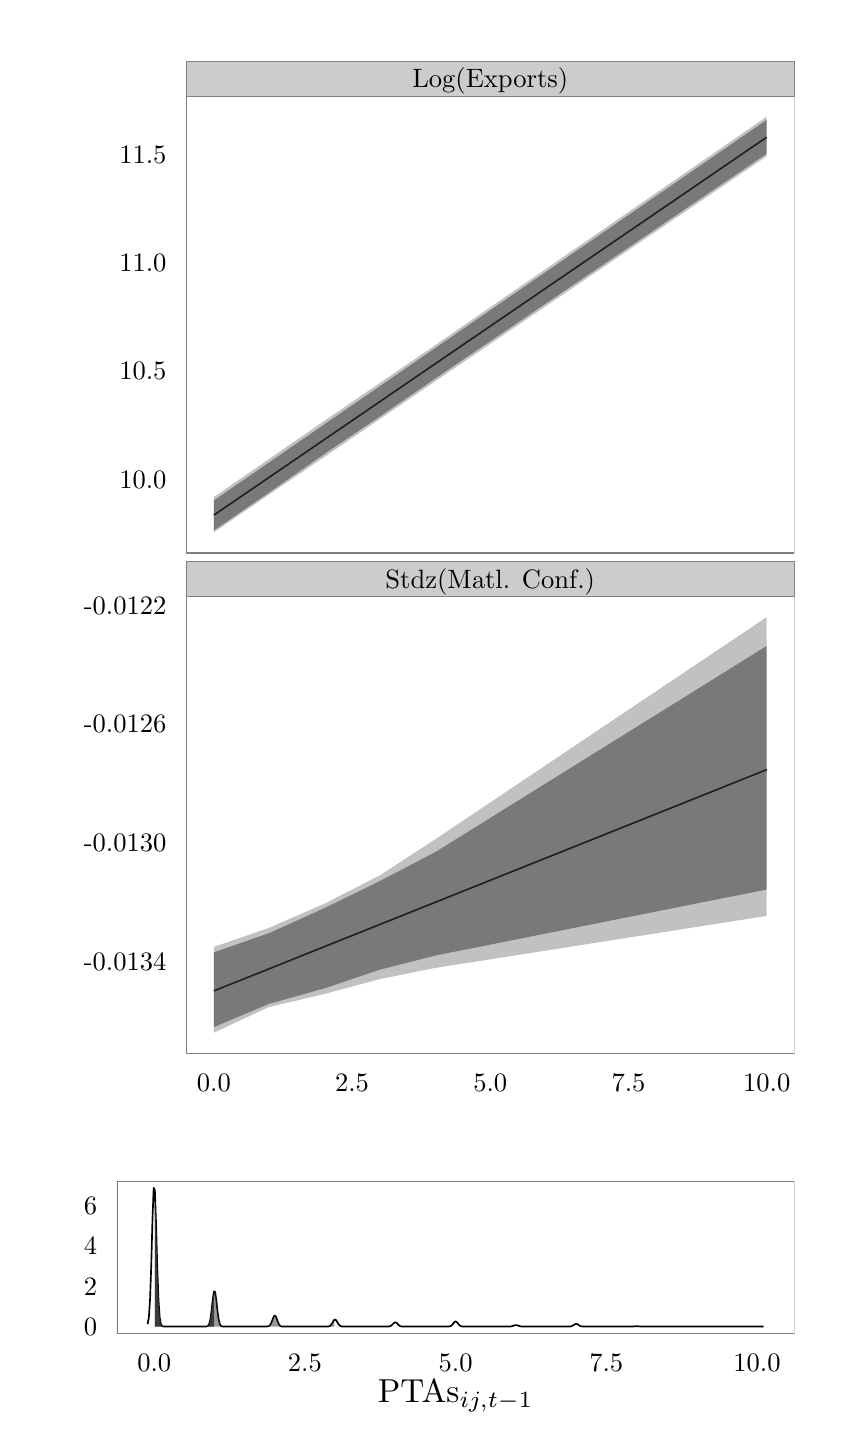
\begin{tikzpicture}[x=1pt,y=1pt]
\definecolor[named]{fillColor}{rgb}{1.00,1.00,1.00}
\path[use as bounding box,fill=fillColor,fill opacity=0.00] (0,0) rectangle (289.08,505.89);
\begin{scope}
\path[clip] (  0.00,101.18) rectangle (289.08,505.89);
\definecolor[named]{drawColor}{rgb}{1.00,1.00,1.00}
\definecolor[named]{fillColor}{rgb}{1.00,1.00,1.00}

\path[draw=drawColor,line width= 0.6pt,line join=round,line cap=round,fill=fillColor] ( -0.00,101.18) rectangle (289.08,505.89);
\end{scope}
\begin{scope}
\path[clip] ( 57.28,316.03) rectangle (277.04,481.21);
\definecolor[named]{fillColor}{rgb}{1.00,1.00,1.00}

\path[fill=fillColor] ( 57.28,316.03) rectangle (277.03,481.21);
\definecolor[named]{drawColor}{rgb}{0.00,0.00,0.00}

\path[draw=drawColor,line width= 0.6pt,line join=round] ( 67.27,329.75) --
	( 87.25,343.40) --
	(107.23,357.06) --
	(127.20,370.71) --
	(147.18,384.37) --
	(267.05,466.30);
\definecolor[named]{fillColor}{rgb}{0.20,0.20,0.20}

\path[fill=fillColor,fill opacity=0.30] ( 67.27,336.26) --
	( 87.25,350.04) --
	(107.23,363.82) --
	(127.20,377.47) --
	(147.18,391.10) --
	(267.05,473.70) --
	(267.05,459.41) --
	(147.18,378.06) --
	(127.20,364.43) --
	(107.23,350.80) --
	( 87.25,337.21) --
	( 67.27,323.54) --
	cycle;
\definecolor[named]{fillColor}{rgb}{0.20,0.20,0.20}

\path[fill=fillColor,fill opacity=0.50] ( 67.27,335.03) --
	( 87.25,348.79) --
	(107.23,362.56) --
	(127.20,376.28) --
	(147.18,390.04) --
	(267.05,472.57) --
	(267.05,460.33) --
	(147.18,379.04) --
	(127.20,365.34) --
	(107.23,351.87) --
	( 87.25,337.93) --
	( 67.27,324.20) --
	cycle;
\definecolor[named]{drawColor}{rgb}{0.50,0.50,0.50}

\path[draw=drawColor,line width= 0.6pt,line join=round,line cap=round] ( 57.28,316.03) rectangle (277.03,481.21);
\end{scope}
\begin{scope}
\path[clip] ( 57.28,135.21) rectangle (277.04,300.39);
\definecolor[named]{fillColor}{rgb}{1.00,1.00,1.00}

\path[fill=fillColor] ( 57.28,135.21) rectangle (277.03,300.39);
\definecolor[named]{drawColor}{rgb}{0.00,0.00,0.00}

\path[draw=drawColor,line width= 0.6pt,line join=round] ( 67.27,157.82) --
	( 87.25,165.81) --
	(107.23,173.81) --
	(127.20,181.80) --
	(147.18,189.80) --
	(267.05,237.77);
\definecolor[named]{fillColor}{rgb}{0.20,0.20,0.20}

\path[fill=fillColor,fill opacity=0.30] ( 67.27,173.70) --
	( 87.25,180.63) --
	(107.23,189.32) --
	(127.20,199.55) --
	(147.18,212.54) --
	(267.05,292.88) --
	(267.05,184.91) --
	(147.18,166.11) --
	(127.20,162.09) --
	(107.23,156.71) --
	( 87.25,152.03) --
	( 67.27,142.72) --
	cycle;
\definecolor[named]{fillColor}{rgb}{0.20,0.20,0.20}

\path[fill=fillColor,fill opacity=0.50] ( 67.27,171.73) --
	( 87.25,178.71) --
	(107.23,187.73) --
	(127.20,197.48) --
	(147.18,207.90) --
	(267.05,282.47) --
	(267.05,194.47) --
	(147.18,170.57) --
	(127.20,165.48) --
	(107.23,158.74) --
	( 87.25,153.16) --
	( 67.27,144.76) --
	cycle;
\definecolor[named]{drawColor}{rgb}{0.50,0.50,0.50}

\path[draw=drawColor,line width= 0.6pt,line join=round,line cap=round] ( 57.28,135.21) rectangle (277.03,300.39);
\end{scope}
\begin{scope}
\path[clip] (  0.00,  0.00) rectangle (289.08,505.89);
\definecolor[named]{drawColor}{rgb}{0.50,0.50,0.50}
\definecolor[named]{fillColor}{rgb}{0.80,0.80,0.80}

\path[draw=drawColor,line width= 0.2pt,line join=round,line cap=round,fill=fillColor] ( 57.28,481.21) rectangle (277.03,493.84);
\definecolor[named]{drawColor}{rgb}{0.00,0.00,0.00}

\node[text=drawColor,anchor=base,inner sep=0pt, outer sep=0pt, scale=  0.96] at (167.16,484.22) {Log(Exports)};
\end{scope}
\begin{scope}
\path[clip] (  0.00,  0.00) rectangle (289.08,505.89);
\definecolor[named]{drawColor}{rgb}{0.50,0.50,0.50}
\definecolor[named]{fillColor}{rgb}{0.80,0.80,0.80}

\path[draw=drawColor,line width= 0.2pt,line join=round,line cap=round,fill=fillColor] ( 57.28,300.39) rectangle (277.03,313.02);
\definecolor[named]{drawColor}{rgb}{0.00,0.00,0.00}

\node[text=drawColor,anchor=base,inner sep=0pt, outer sep=0pt, scale=  0.96] at (167.16,303.40) {Stdz(Matl. Conf.)};
\end{scope}
\begin{scope}
\path[clip] (  0.00,  0.00) rectangle (289.08,505.89);
\definecolor[named]{drawColor}{rgb}{0.00,0.00,0.00}

\node[text=drawColor,anchor=base east,inner sep=0pt, outer sep=0pt, scale=  0.96] at ( 50.17,339.52) {10.0};

\node[text=drawColor,anchor=base east,inner sep=0pt, outer sep=0pt, scale=  0.96] at ( 50.17,378.64) {10.5};

\node[text=drawColor,anchor=base east,inner sep=0pt, outer sep=0pt, scale=  0.96] at ( 50.17,417.76) {11.0};

\node[text=drawColor,anchor=base east,inner sep=0pt, outer sep=0pt, scale=  0.96] at ( 50.17,456.88) {11.5};
\end{scope}
\begin{scope}
\path[clip] (  0.00,  0.00) rectangle (289.08,505.89);
\definecolor[named]{drawColor}{rgb}{0.00,0.00,0.00}

\node[text=drawColor,anchor=base east,inner sep=0pt, outer sep=0pt, scale=  0.96] at ( 50.17,165.28) {-0.0134};

\node[text=drawColor,anchor=base east,inner sep=0pt, outer sep=0pt, scale=  0.96] at ( 50.17,208.18) {-0.0130};

\node[text=drawColor,anchor=base east,inner sep=0pt, outer sep=0pt, scale=  0.96] at ( 50.17,251.09) {-0.0126};

\node[text=drawColor,anchor=base east,inner sep=0pt, outer sep=0pt, scale=  0.96] at ( 50.17,293.99) {-0.0122};
\end{scope}
\begin{scope}
\path[clip] (  0.00,  0.00) rectangle (289.08,505.89);
\definecolor[named]{drawColor}{rgb}{0.00,0.00,0.00}

\node[text=drawColor,anchor=base,inner sep=0pt, outer sep=0pt, scale=  0.96] at ( 67.27,121.49) {0.0};

\node[text=drawColor,anchor=base,inner sep=0pt, outer sep=0pt, scale=  0.96] at (117.21,121.49) {2.5};

\node[text=drawColor,anchor=base,inner sep=0pt, outer sep=0pt, scale=  0.96] at (167.16,121.49) {5.0};

\node[text=drawColor,anchor=base,inner sep=0pt, outer sep=0pt, scale=  0.96] at (217.10,121.49) {7.5};

\node[text=drawColor,anchor=base,inner sep=0pt, outer sep=0pt, scale=  0.96] at (267.05,121.49) {10.0};
\end{scope}
\begin{scope}
\path[clip] (  0.00,  0.00) rectangle (289.08,101.18);
\definecolor[named]{drawColor}{rgb}{1.00,1.00,1.00}
\definecolor[named]{fillColor}{rgb}{1.00,1.00,1.00}

\path[draw=drawColor,line width= 0.6pt,line join=round,line cap=round,fill=fillColor] (  0.00,  0.00) rectangle (289.08,101.18);
\end{scope}
\begin{scope}
\path[clip] ( 32.22, 34.03) rectangle (277.04, 89.13);
\definecolor[named]{fillColor}{rgb}{1.00,1.00,1.00}

\path[fill=fillColor] ( 32.22, 34.03) rectangle (277.03, 89.13);
\definecolor[named]{drawColor}{rgb}{0.00,0.00,0.00}

\path[draw=drawColor,line width= 0.6pt,line join=round] ( 43.35, 37.41) --
	( 43.79, 39.86) --
	( 44.22, 46.35) --
	( 44.66, 58.83) --
	( 45.09, 75.08) --
	( 45.53, 86.63) --
	( 45.96, 85.82) --
	( 46.40, 73.56) --
	( 46.83, 57.94) --
	( 47.27, 46.13) --
	( 47.70, 39.88) --
	( 48.14, 37.45) --
	( 48.58, 36.73) --
	( 49.01, 36.57) --
	( 49.45, 36.54) --
	( 49.88, 36.54) --
	( 50.32, 36.54) --
	( 50.75, 36.54) --
	( 51.19, 36.54) --
	( 51.62, 36.54) --
	( 52.06, 36.54) --
	( 52.50, 36.54) --
	( 52.93, 36.54) --
	( 53.37, 36.54) --
	( 53.80, 36.54) --
	( 54.24, 36.54) --
	( 54.67, 36.54) --
	( 55.11, 36.54) --
	( 55.54, 36.54) --
	( 55.98, 36.54) --
	( 56.42, 36.54) --
	( 56.85, 36.54) --
	( 57.29, 36.54) --
	( 57.72, 36.54) --
	( 58.16, 36.54) --
	( 58.59, 36.54) --
	( 59.03, 36.54) --
	( 59.46, 36.54) --
	( 59.90, 36.54) --
	( 60.34, 36.54) --
	( 60.77, 36.54) --
	( 61.21, 36.54) --
	( 61.64, 36.54) --
	( 62.08, 36.54) --
	( 62.51, 36.54) --
	( 62.95, 36.54) --
	( 63.38, 36.54) --
	( 63.82, 36.54) --
	( 64.26, 36.54) --
	( 64.69, 36.57) --
	( 65.13, 36.73) --
	( 65.56, 37.33) --
	( 66.00, 38.98) --
	( 66.43, 42.17) --
	( 66.87, 46.26) --
	( 67.30, 49.23) --
	( 67.74, 49.11) --
	( 68.17, 46.01) --
	( 68.61, 41.96) --
	( 69.05, 38.89) --
	( 69.48, 37.30) --
	( 69.92, 36.73) --
	( 70.35, 36.57) --
	( 70.79, 36.54) --
	( 71.22, 36.54) --
	( 71.66, 36.54) --
	( 72.09, 36.54) --
	( 72.53, 36.54) --
	( 72.97, 36.54) --
	( 73.40, 36.54) --
	( 73.84, 36.54) --
	( 74.27, 36.54) --
	( 74.71, 36.54) --
	( 75.14, 36.54) --
	( 75.58, 36.54) --
	( 76.01, 36.54) --
	( 76.45, 36.54) --
	( 76.89, 36.54) --
	( 77.32, 36.54) --
	( 77.76, 36.54) --
	( 78.19, 36.54) --
	( 78.63, 36.54) --
	( 79.06, 36.54) --
	( 79.50, 36.54) --
	( 79.93, 36.54) --
	( 80.37, 36.54) --
	( 80.81, 36.54) --
	( 81.24, 36.54) --
	( 81.68, 36.54) --
	( 82.11, 36.54) --
	( 82.55, 36.54) --
	( 82.98, 36.54) --
	( 83.42, 36.54) --
	( 83.85, 36.54) --
	( 84.29, 36.54) --
	( 84.73, 36.54) --
	( 85.16, 36.54) --
	( 85.60, 36.54) --
	( 86.03, 36.54) --
	( 86.47, 36.56) --
	( 86.90, 36.62) --
	( 87.34, 36.83) --
	( 87.77, 37.34) --
	( 88.21, 38.29) --
	( 88.65, 39.50) --
	( 89.08, 40.41) --
	( 89.52, 40.43) --
	( 89.95, 39.51) --
	( 90.39, 38.25) --
	( 90.82, 37.28) --
	( 91.26, 36.78) --
	( 91.69, 36.59) --
	( 92.13, 36.55) --
	( 92.56, 36.54) --
	( 93.00, 36.54) --
	( 93.44, 36.54) --
	( 93.87, 36.54) --
	( 94.31, 36.54) --
	( 94.74, 36.54) --
	( 95.18, 36.54) --
	( 95.61, 36.54) --
	( 96.05, 36.54) --
	( 96.48, 36.54) --
	( 96.92, 36.54) --
	( 97.36, 36.54) --
	( 97.79, 36.54) --
	( 98.23, 36.54) --
	( 98.66, 36.54) --
	( 99.10, 36.54) --
	( 99.53, 36.54) --
	( 99.97, 36.54) --
	(100.40, 36.54) --
	(100.84, 36.54) --
	(101.28, 36.54) --
	(101.71, 36.54) --
	(102.15, 36.54) --
	(102.58, 36.54) --
	(103.02, 36.54) --
	(103.45, 36.54) --
	(103.89, 36.54) --
	(104.32, 36.54) --
	(104.76, 36.54) --
	(105.20, 36.54) --
	(105.63, 36.54) --
	(106.07, 36.54) --
	(106.50, 36.54) --
	(106.94, 36.54) --
	(107.37, 36.54) --
	(107.81, 36.54) --
	(108.24, 36.55) --
	(108.68, 36.58) --
	(109.12, 36.70) --
	(109.55, 37.03) --
	(109.99, 37.66) --
	(110.42, 38.47) --
	(110.86, 39.04) --
	(111.29, 39.01) --
	(111.73, 38.41) --
	(112.16, 37.63) --
	(112.60, 37.04) --
	(113.03, 36.71) --
	(113.47, 36.59) --
	(113.91, 36.55) --
	(114.34, 36.54) --
	(114.78, 36.54) --
	(115.21, 36.54) --
	(115.65, 36.54) --
	(116.08, 36.54) --
	(116.52, 36.54) --
	(116.95, 36.54) --
	(117.39, 36.54) --
	(117.83, 36.54) --
	(118.26, 36.54) --
	(118.70, 36.54) --
	(119.13, 36.54) --
	(119.57, 36.54) --
	(120.00, 36.54) --
	(120.44, 36.54) --
	(120.87, 36.54) --
	(121.31, 36.54) --
	(121.75, 36.54) --
	(122.18, 36.54) --
	(122.62, 36.54) --
	(123.05, 36.54) --
	(123.49, 36.54) --
	(123.92, 36.54) --
	(124.36, 36.54) --
	(124.79, 36.54) --
	(125.23, 36.54) --
	(125.67, 36.54) --
	(126.10, 36.54) --
	(126.54, 36.54) --
	(126.97, 36.54) --
	(127.41, 36.54) --
	(127.84, 36.54) --
	(128.28, 36.54) --
	(128.71, 36.54) --
	(129.15, 36.54) --
	(129.59, 36.54) --
	(130.02, 36.54) --
	(130.46, 36.57) --
	(130.89, 36.64) --
	(131.33, 36.84) --
	(131.76, 37.20) --
	(132.20, 37.67) --
	(132.63, 38.03) --
	(133.07, 38.04) --
	(133.50, 37.68) --
	(133.94, 37.20) --
	(134.38, 36.83) --
	(134.81, 36.63) --
	(135.25, 36.56) --
	(135.68, 36.54) --
	(136.12, 36.54) --
	(136.55, 36.54) --
	(136.99, 36.54) --
	(137.42, 36.54) --
	(137.86, 36.54) --
	(138.30, 36.54) --
	(138.73, 36.54) --
	(139.17, 36.54) --
	(139.60, 36.54) --
	(140.04, 36.54) --
	(140.47, 36.54) --
	(140.91, 36.54) --
	(141.34, 36.54) --
	(141.78, 36.54) --
	(142.22, 36.54) --
	(142.65, 36.54) --
	(143.09, 36.54) --
	(143.52, 36.54) --
	(143.96, 36.54) --
	(144.39, 36.54) --
	(144.83, 36.54) --
	(145.26, 36.54) --
	(145.70, 36.54) --
	(146.14, 36.54) --
	(146.57, 36.54) --
	(147.01, 36.54) --
	(147.44, 36.54) --
	(147.88, 36.54) --
	(148.31, 36.54) --
	(148.75, 36.54) --
	(149.18, 36.54) --
	(149.62, 36.54) --
	(150.06, 36.54) --
	(150.49, 36.54) --
	(150.93, 36.54) --
	(151.36, 36.54) --
	(151.80, 36.55) --
	(152.23, 36.57) --
	(152.67, 36.66) --
	(153.10, 36.89) --
	(153.54, 37.33) --
	(153.98, 37.90) --
	(154.41, 38.34) --
	(154.85, 38.34) --
	(155.28, 37.90) --
	(155.72, 37.33) --
	(156.15, 36.89) --
	(156.59, 36.66) --
	(157.02, 36.57) --
	(157.46, 36.55) --
	(157.89, 36.54) --
	(158.33, 36.54) --
	(158.77, 36.54) --
	(159.20, 36.54) --
	(159.64, 36.54) --
	(160.07, 36.54) --
	(160.51, 36.54) --
	(160.94, 36.54) --
	(161.38, 36.54) --
	(161.81, 36.54) --
	(162.25, 36.54) --
	(162.69, 36.54) --
	(163.12, 36.54) --
	(163.56, 36.54) --
	(163.99, 36.54) --
	(164.43, 36.54) --
	(164.86, 36.54) --
	(165.30, 36.54) --
	(165.73, 36.54) --
	(166.17, 36.54) --
	(166.61, 36.54) --
	(167.04, 36.54) --
	(167.48, 36.54) --
	(167.91, 36.54) --
	(168.35, 36.54) --
	(168.78, 36.54) --
	(169.22, 36.54) --
	(169.65, 36.54) --
	(170.09, 36.54) --
	(170.53, 36.54) --
	(170.96, 36.54) --
	(171.40, 36.54) --
	(171.83, 36.54) --
	(172.27, 36.54) --
	(172.70, 36.54) --
	(173.14, 36.54) --
	(173.57, 36.54) --
	(174.01, 36.55) --
	(174.45, 36.57) --
	(174.88, 36.64) --
	(175.32, 36.77) --
	(175.75, 36.94) --
	(176.19, 37.06) --
	(176.62, 37.06) --
	(177.06, 36.94) --
	(177.49, 36.77) --
	(177.93, 36.64) --
	(178.36, 36.57) --
	(178.80, 36.55) --
	(179.24, 36.54) --
	(179.67, 36.54) --
	(180.11, 36.54) --
	(180.54, 36.54) --
	(180.98, 36.54) --
	(181.41, 36.54) --
	(181.85, 36.54) --
	(182.28, 36.54) --
	(182.72, 36.54) --
	(183.16, 36.54) --
	(183.59, 36.54) --
	(184.03, 36.54) --
	(184.46, 36.54) --
	(184.90, 36.54) --
	(185.33, 36.54) --
	(185.77, 36.54) --
	(186.20, 36.54) --
	(186.64, 36.54) --
	(187.08, 36.54) --
	(187.51, 36.54) --
	(187.95, 36.54) --
	(188.38, 36.54) --
	(188.82, 36.54) --
	(189.25, 36.54) --
	(189.69, 36.54) --
	(190.12, 36.54) --
	(190.56, 36.54) --
	(191.00, 36.54) --
	(191.43, 36.54) --
	(191.87, 36.54) --
	(192.30, 36.54) --
	(192.74, 36.54) --
	(193.17, 36.54) --
	(193.61, 36.54) --
	(194.04, 36.54) --
	(194.48, 36.54) --
	(194.92, 36.54) --
	(195.35, 36.54) --
	(195.79, 36.56) --
	(196.22, 36.61) --
	(196.66, 36.73) --
	(197.09, 36.96) --
	(197.53, 37.26) --
	(197.96, 37.49) --
	(198.40, 37.50) --
	(198.83, 37.28) --
	(199.27, 36.97) --
	(199.71, 36.73) --
	(200.14, 36.60) --
	(200.58, 36.55) --
	(201.01, 36.54) --
	(201.45, 36.54) --
	(201.88, 36.54) --
	(202.32, 36.54) --
	(202.75, 36.54) --
	(203.19, 36.54) --
	(203.63, 36.54) --
	(204.06, 36.54) --
	(204.50, 36.54) --
	(204.93, 36.54) --
	(205.37, 36.54) --
	(205.80, 36.54) --
	(206.24, 36.54) --
	(206.67, 36.54) --
	(207.11, 36.54) --
	(207.55, 36.54) --
	(207.98, 36.54) --
	(208.42, 36.54) --
	(208.85, 36.54) --
	(209.29, 36.54) --
	(209.72, 36.54) --
	(210.16, 36.54) --
	(210.59, 36.54) --
	(211.03, 36.54) --
	(211.47, 36.54) --
	(211.90, 36.54) --
	(212.34, 36.54) --
	(212.77, 36.54) --
	(213.21, 36.54) --
	(213.64, 36.54) --
	(214.08, 36.54) --
	(214.51, 36.54) --
	(214.95, 36.54) --
	(215.39, 36.54) --
	(215.82, 36.54) --
	(216.26, 36.54) --
	(216.69, 36.54) --
	(217.13, 36.54) --
	(217.56, 36.54) --
	(218.00, 36.55) --
	(218.43, 36.56) --
	(218.87, 36.58) --
	(219.31, 36.62) --
	(219.74, 36.64) --
	(220.18, 36.64) --
	(220.61, 36.62) --
	(221.05, 36.59) --
	(221.48, 36.56) --
	(221.92, 36.55) --
	(222.35, 36.54) --
	(222.79, 36.54) --
	(223.22, 36.54) --
	(223.66, 36.54) --
	(224.10, 36.54) --
	(224.53, 36.54) --
	(224.97, 36.54) --
	(225.40, 36.54) --
	(225.84, 36.54) --
	(226.27, 36.54) --
	(226.71, 36.54) --
	(227.14, 36.54) --
	(227.58, 36.54) --
	(228.02, 36.54) --
	(228.45, 36.54) --
	(228.89, 36.54) --
	(229.32, 36.54) --
	(229.76, 36.54) --
	(230.19, 36.54) --
	(230.63, 36.54) --
	(231.06, 36.54) --
	(231.50, 36.54) --
	(231.94, 36.54) --
	(232.37, 36.54) --
	(232.81, 36.54) --
	(233.24, 36.54) --
	(233.68, 36.54) --
	(234.11, 36.54) --
	(234.55, 36.54) --
	(234.98, 36.54) --
	(235.42, 36.54) --
	(235.86, 36.54) --
	(236.29, 36.54) --
	(236.73, 36.54) --
	(237.16, 36.54) --
	(237.60, 36.54) --
	(238.03, 36.54) --
	(238.47, 36.54) --
	(238.90, 36.54) --
	(239.34, 36.54) --
	(239.78, 36.54) --
	(240.21, 36.54) --
	(240.65, 36.55) --
	(241.08, 36.55) --
	(241.52, 36.56) --
	(241.95, 36.56) --
	(242.39, 36.55) --
	(242.82, 36.55) --
	(243.26, 36.54) --
	(243.69, 36.54) --
	(244.13, 36.54) --
	(244.57, 36.54) --
	(245.00, 36.54) --
	(245.44, 36.54) --
	(245.87, 36.54) --
	(246.31, 36.54) --
	(246.74, 36.54) --
	(247.18, 36.54) --
	(247.61, 36.54) --
	(248.05, 36.54) --
	(248.49, 36.54) --
	(248.92, 36.54) --
	(249.36, 36.54) --
	(249.79, 36.54) --
	(250.23, 36.54) --
	(250.66, 36.54) --
	(251.10, 36.54) --
	(251.53, 36.54) --
	(251.97, 36.54) --
	(252.41, 36.54) --
	(252.84, 36.54) --
	(253.28, 36.54) --
	(253.71, 36.54) --
	(254.15, 36.54) --
	(254.58, 36.54) --
	(255.02, 36.54) --
	(255.45, 36.54) --
	(255.89, 36.54) --
	(256.33, 36.54) --
	(256.76, 36.54) --
	(257.20, 36.54) --
	(257.63, 36.54) --
	(258.07, 36.54) --
	(258.50, 36.54) --
	(258.94, 36.54) --
	(259.37, 36.54) --
	(259.81, 36.54) --
	(260.25, 36.54) --
	(260.68, 36.54) --
	(261.12, 36.54) --
	(261.55, 36.54) --
	(261.99, 36.54) --
	(262.42, 36.54) --
	(262.86, 36.54) --
	(263.29, 36.55) --
	(263.73, 36.55) --
	(264.16, 36.54) --
	(264.60, 36.54) --
	(265.04, 36.54) --
	(265.47, 36.54) --
	(265.91, 36.54);
\definecolor[named]{fillColor}{rgb}{0.20,0.20,0.20}

\path[fill=fillColor,fill opacity=0.50] ( 45.96, 85.82) --
	( 46.40, 73.56) --
	( 46.83, 57.94) --
	( 47.27, 46.13) --
	( 47.70, 39.88) --
	( 48.14, 37.45) --
	( 48.58, 36.73) --
	( 49.01, 36.57) --
	( 49.45, 36.54) --
	( 49.88, 36.54) --
	( 50.32, 36.54) --
	( 50.75, 36.54) --
	( 51.19, 36.54) --
	( 51.62, 36.54) --
	( 52.06, 36.54) --
	( 52.50, 36.54) --
	( 52.93, 36.54) --
	( 53.37, 36.54) --
	( 53.80, 36.54) --
	( 54.24, 36.54) --
	( 54.67, 36.54) --
	( 55.11, 36.54) --
	( 55.54, 36.54) --
	( 55.98, 36.54) --
	( 56.42, 36.54) --
	( 56.85, 36.54) --
	( 57.29, 36.54) --
	( 57.72, 36.54) --
	( 58.16, 36.54) --
	( 58.59, 36.54) --
	( 59.03, 36.54) --
	( 59.46, 36.54) --
	( 59.90, 36.54) --
	( 60.34, 36.54) --
	( 60.77, 36.54) --
	( 61.21, 36.54) --
	( 61.64, 36.54) --
	( 62.08, 36.54) --
	( 62.51, 36.54) --
	( 62.95, 36.54) --
	( 63.38, 36.54) --
	( 63.82, 36.54) --
	( 64.26, 36.54) --
	( 64.69, 36.57) --
	( 65.13, 36.73) --
	( 65.56, 37.33) --
	( 66.00, 38.98) --
	( 66.43, 42.17) --
	( 66.87, 46.26) --
	( 67.30, 49.23) --
	( 67.74, 49.11) --
	( 68.17, 46.01) --
	( 68.61, 41.96) --
	( 69.05, 38.89) --
	( 69.48, 37.30) --
	( 69.92, 36.73) --
	( 70.35, 36.57) --
	( 70.79, 36.54) --
	( 71.22, 36.54) --
	( 71.66, 36.54) --
	( 72.09, 36.54) --
	( 72.53, 36.54) --
	( 72.97, 36.54) --
	( 73.40, 36.54) --
	( 73.84, 36.54) --
	( 74.27, 36.54) --
	( 74.71, 36.54) --
	( 75.14, 36.54) --
	( 75.58, 36.54) --
	( 76.01, 36.54) --
	( 76.45, 36.54) --
	( 76.89, 36.54) --
	( 77.32, 36.54) --
	( 77.76, 36.54) --
	( 78.19, 36.54) --
	( 78.63, 36.54) --
	( 79.06, 36.54) --
	( 79.50, 36.54) --
	( 79.93, 36.54) --
	( 80.37, 36.54) --
	( 80.81, 36.54) --
	( 81.24, 36.54) --
	( 81.68, 36.54) --
	( 82.11, 36.54) --
	( 82.55, 36.54) --
	( 82.98, 36.54) --
	( 83.42, 36.54) --
	( 83.85, 36.54) --
	( 84.29, 36.54) --
	( 84.73, 36.54) --
	( 85.16, 36.54) --
	( 85.60, 36.54) --
	( 86.03, 36.54) --
	( 86.47, 36.56) --
	( 86.90, 36.62) --
	( 87.34, 36.83) --
	( 87.77, 37.34) --
	( 88.21, 38.29) --
	( 88.65, 39.50) --
	( 89.08, 40.41) --
	( 89.52, 40.43) --
	( 89.95, 39.51) --
	( 90.39, 38.25) --
	( 90.82, 37.28) --
	( 91.26, 36.78) --
	( 91.69, 36.59) --
	( 92.13, 36.55) --
	( 92.56, 36.54) --
	( 93.00, 36.54) --
	( 93.44, 36.54) --
	( 93.87, 36.54) --
	( 94.31, 36.54) --
	( 94.74, 36.54) --
	( 95.18, 36.54) --
	( 95.61, 36.54) --
	( 96.05, 36.54) --
	( 96.48, 36.54) --
	( 96.92, 36.54) --
	( 97.36, 36.54) --
	( 97.79, 36.54) --
	( 98.23, 36.54) --
	( 98.66, 36.54) --
	( 99.10, 36.54) --
	( 99.53, 36.54) --
	( 99.97, 36.54) --
	(100.40, 36.54) --
	(100.84, 36.54) --
	(101.28, 36.54) --
	(101.71, 36.54) --
	(102.15, 36.54) --
	(102.58, 36.54) --
	(103.02, 36.54) --
	(103.45, 36.54) --
	(103.89, 36.54) --
	(104.32, 36.54) --
	(104.76, 36.54) --
	(105.20, 36.54) --
	(105.63, 36.54) --
	(106.07, 36.54) --
	(106.50, 36.54) --
	(106.94, 36.54) --
	(107.37, 36.54) --
	(107.81, 36.54) --
	(108.24, 36.55) --
	(108.68, 36.58) --
	(109.12, 36.70) --
	(109.55, 37.03) --
	(109.99, 37.66) --
	(110.42, 38.47) --
	(110.86, 39.04) --
	(110.86, 36.54) --
	(110.42, 36.54) --
	(109.99, 36.54) --
	(109.55, 36.54) --
	(109.12, 36.54) --
	(108.68, 36.54) --
	(108.24, 36.54) --
	(107.81, 36.54) --
	(107.37, 36.54) --
	(106.94, 36.54) --
	(106.50, 36.54) --
	(106.07, 36.54) --
	(105.63, 36.54) --
	(105.20, 36.54) --
	(104.76, 36.54) --
	(104.32, 36.54) --
	(103.89, 36.54) --
	(103.45, 36.54) --
	(103.02, 36.54) --
	(102.58, 36.54) --
	(102.15, 36.54) --
	(101.71, 36.54) --
	(101.28, 36.54) --
	(100.84, 36.54) --
	(100.40, 36.54) --
	( 99.97, 36.54) --
	( 99.53, 36.54) --
	( 99.10, 36.54) --
	( 98.66, 36.54) --
	( 98.23, 36.54) --
	( 97.79, 36.54) --
	( 97.36, 36.54) --
	( 96.92, 36.54) --
	( 96.48, 36.54) --
	( 96.05, 36.54) --
	( 95.61, 36.54) --
	( 95.18, 36.54) --
	( 94.74, 36.54) --
	( 94.31, 36.54) --
	( 93.87, 36.54) --
	( 93.44, 36.54) --
	( 93.00, 36.54) --
	( 92.56, 36.54) --
	( 92.13, 36.54) --
	( 91.69, 36.54) --
	( 91.26, 36.54) --
	( 90.82, 36.54) --
	( 90.39, 36.54) --
	( 89.95, 36.54) --
	( 89.52, 36.54) --
	( 89.08, 36.54) --
	( 88.65, 36.54) --
	( 88.21, 36.54) --
	( 87.77, 36.54) --
	( 87.34, 36.54) --
	( 86.90, 36.54) --
	( 86.47, 36.54) --
	( 86.03, 36.54) --
	( 85.60, 36.54) --
	( 85.16, 36.54) --
	( 84.73, 36.54) --
	( 84.29, 36.54) --
	( 83.85, 36.54) --
	( 83.42, 36.54) --
	( 82.98, 36.54) --
	( 82.55, 36.54) --
	( 82.11, 36.54) --
	( 81.68, 36.54) --
	( 81.24, 36.54) --
	( 80.81, 36.54) --
	( 80.37, 36.54) --
	( 79.93, 36.54) --
	( 79.50, 36.54) --
	( 79.06, 36.54) --
	( 78.63, 36.54) --
	( 78.19, 36.54) --
	( 77.76, 36.54) --
	( 77.32, 36.54) --
	( 76.89, 36.54) --
	( 76.45, 36.54) --
	( 76.01, 36.54) --
	( 75.58, 36.54) --
	( 75.14, 36.54) --
	( 74.71, 36.54) --
	( 74.27, 36.54) --
	( 73.84, 36.54) --
	( 73.40, 36.54) --
	( 72.97, 36.54) --
	( 72.53, 36.54) --
	( 72.09, 36.54) --
	( 71.66, 36.54) --
	( 71.22, 36.54) --
	( 70.79, 36.54) --
	( 70.35, 36.54) --
	( 69.92, 36.54) --
	( 69.48, 36.54) --
	( 69.05, 36.54) --
	( 68.61, 36.54) --
	( 68.17, 36.54) --
	( 67.74, 36.54) --
	( 67.30, 36.54) --
	( 66.87, 36.54) --
	( 66.43, 36.54) --
	( 66.00, 36.54) --
	( 65.56, 36.54) --
	( 65.13, 36.54) --
	( 64.69, 36.54) --
	( 64.26, 36.54) --
	( 63.82, 36.54) --
	( 63.38, 36.54) --
	( 62.95, 36.54) --
	( 62.51, 36.54) --
	( 62.08, 36.54) --
	( 61.64, 36.54) --
	( 61.21, 36.54) --
	( 60.77, 36.54) --
	( 60.34, 36.54) --
	( 59.90, 36.54) --
	( 59.46, 36.54) --
	( 59.03, 36.54) --
	( 58.59, 36.54) --
	( 58.16, 36.54) --
	( 57.72, 36.54) --
	( 57.29, 36.54) --
	( 56.85, 36.54) --
	( 56.42, 36.54) --
	( 55.98, 36.54) --
	( 55.54, 36.54) --
	( 55.11, 36.54) --
	( 54.67, 36.54) --
	( 54.24, 36.54) --
	( 53.80, 36.54) --
	( 53.37, 36.54) --
	( 52.93, 36.54) --
	( 52.50, 36.54) --
	( 52.06, 36.54) --
	( 51.62, 36.54) --
	( 51.19, 36.54) --
	( 50.75, 36.54) --
	( 50.32, 36.54) --
	( 49.88, 36.54) --
	( 49.45, 36.54) --
	( 49.01, 36.54) --
	( 48.58, 36.54) --
	( 48.14, 36.54) --
	( 47.70, 36.54) --
	( 47.27, 36.54) --
	( 46.83, 36.54) --
	( 46.40, 36.54) --
	( 45.96, 36.54) --
	cycle;
\definecolor[named]{fillColor}{rgb}{0.20,0.20,0.20}

\path[fill=fillColor,fill opacity=0.90] ( 45.96, 85.82) --
	( 46.40, 73.56) --
	( 46.83, 57.94) --
	( 47.27, 46.13) --
	( 47.70, 39.88) --
	( 48.14, 37.45) --
	( 48.58, 36.73) --
	( 49.01, 36.57) --
	( 49.45, 36.54) --
	( 49.88, 36.54) --
	( 50.32, 36.54) --
	( 50.75, 36.54) --
	( 51.19, 36.54) --
	( 51.62, 36.54) --
	( 52.06, 36.54) --
	( 52.50, 36.54) --
	( 52.93, 36.54) --
	( 53.37, 36.54) --
	( 53.80, 36.54) --
	( 54.24, 36.54) --
	( 54.67, 36.54) --
	( 55.11, 36.54) --
	( 55.54, 36.54) --
	( 55.98, 36.54) --
	( 56.42, 36.54) --
	( 56.85, 36.54) --
	( 57.29, 36.54) --
	( 57.72, 36.54) --
	( 58.16, 36.54) --
	( 58.59, 36.54) --
	( 59.03, 36.54) --
	( 59.46, 36.54) --
	( 59.90, 36.54) --
	( 60.34, 36.54) --
	( 60.77, 36.54) --
	( 61.21, 36.54) --
	( 61.64, 36.54) --
	( 62.08, 36.54) --
	( 62.51, 36.54) --
	( 62.95, 36.54) --
	( 63.38, 36.54) --
	( 63.82, 36.54) --
	( 64.26, 36.54) --
	( 64.69, 36.57) --
	( 65.13, 36.73) --
	( 65.56, 37.33) --
	( 66.00, 38.98) --
	( 66.43, 42.17) --
	( 66.87, 46.26) --
	( 67.30, 49.23) --
	( 67.30, 36.54) --
	( 66.87, 36.54) --
	( 66.43, 36.54) --
	( 66.00, 36.54) --
	( 65.56, 36.54) --
	( 65.13, 36.54) --
	( 64.69, 36.54) --
	( 64.26, 36.54) --
	( 63.82, 36.54) --
	( 63.38, 36.54) --
	( 62.95, 36.54) --
	( 62.51, 36.54) --
	( 62.08, 36.54) --
	( 61.64, 36.54) --
	( 61.21, 36.54) --
	( 60.77, 36.54) --
	( 60.34, 36.54) --
	( 59.90, 36.54) --
	( 59.46, 36.54) --
	( 59.03, 36.54) --
	( 58.59, 36.54) --
	( 58.16, 36.54) --
	( 57.72, 36.54) --
	( 57.29, 36.54) --
	( 56.85, 36.54) --
	( 56.42, 36.54) --
	( 55.98, 36.54) --
	( 55.54, 36.54) --
	( 55.11, 36.54) --
	( 54.67, 36.54) --
	( 54.24, 36.54) --
	( 53.80, 36.54) --
	( 53.37, 36.54) --
	( 52.93, 36.54) --
	( 52.50, 36.54) --
	( 52.06, 36.54) --
	( 51.62, 36.54) --
	( 51.19, 36.54) --
	( 50.75, 36.54) --
	( 50.32, 36.54) --
	( 49.88, 36.54) --
	( 49.45, 36.54) --
	( 49.01, 36.54) --
	( 48.58, 36.54) --
	( 48.14, 36.54) --
	( 47.70, 36.54) --
	( 47.27, 36.54) --
	( 46.83, 36.54) --
	( 46.40, 36.54) --
	( 45.96, 36.54) --
	cycle;
\definecolor[named]{drawColor}{rgb}{0.50,0.50,0.50}

\path[draw=drawColor,line width= 0.6pt,line join=round,line cap=round] ( 32.22, 34.03) rectangle (277.03, 89.13);
\end{scope}
\begin{scope}
\path[clip] (  0.00,  0.00) rectangle (289.08,505.89);
\definecolor[named]{drawColor}{rgb}{0.00,0.00,0.00}

\node[text=drawColor,anchor=base east,inner sep=0pt, outer sep=0pt, scale=  0.96] at ( 25.11, 33.23) {0};

\node[text=drawColor,anchor=base east,inner sep=0pt, outer sep=0pt, scale=  0.96] at ( 25.11, 47.81) {2};

\node[text=drawColor,anchor=base east,inner sep=0pt, outer sep=0pt, scale=  0.96] at ( 25.11, 62.40) {4};

\node[text=drawColor,anchor=base east,inner sep=0pt, outer sep=0pt, scale=  0.96] at ( 25.11, 76.98) {6};
\end{scope}
\begin{scope}
\path[clip] (  0.00,  0.00) rectangle (289.08,505.89);
\definecolor[named]{drawColor}{rgb}{0.00,0.00,0.00}

\node[text=drawColor,anchor=base,inner sep=0pt, outer sep=0pt, scale=  0.96] at ( 45.73, 20.31) {0.0};

\node[text=drawColor,anchor=base,inner sep=0pt, outer sep=0pt, scale=  0.96] at (100.18, 20.31) {2.5};

\node[text=drawColor,anchor=base,inner sep=0pt, outer sep=0pt, scale=  0.96] at (154.63, 20.31) {5.0};

\node[text=drawColor,anchor=base,inner sep=0pt, outer sep=0pt, scale=  0.96] at (209.08, 20.31) {7.5};

\node[text=drawColor,anchor=base,inner sep=0pt, outer sep=0pt, scale=  0.96] at (263.53, 20.31) {10.0};
\end{scope}
\begin{scope}
\path[clip] (  0.00,  0.00) rectangle (289.08,505.89);
\definecolor[named]{drawColor}{rgb}{0.00,0.00,0.00}

\node[text=drawColor,anchor=base,inner sep=0pt, outer sep=0pt, scale=  1.20] at (154.63,  9.03) {PTAs$_{ij, t-1}$};
\end{scope}
\end{tikzpicture}
}  &
      \resizebox{.45\textwidth}{!}{% Created by tikzDevice version 0.7.0 on 2015-07-01 08:58:18
% !TEX encoding = UTF-8 Unicode
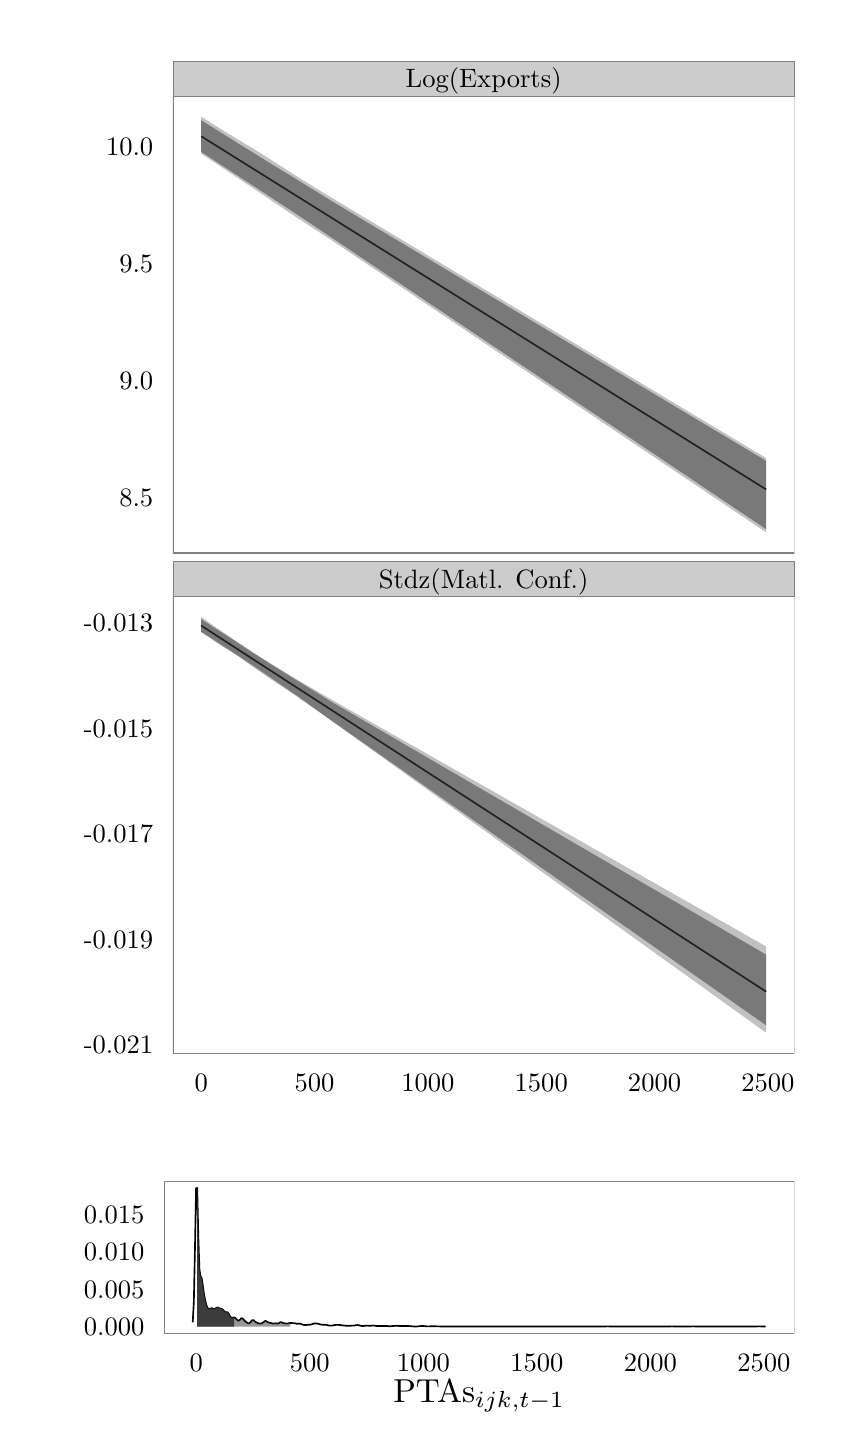
\begin{tikzpicture}[x=1pt,y=1pt]
\definecolor[named]{fillColor}{rgb}{1.00,1.00,1.00}
\path[use as bounding box,fill=fillColor,fill opacity=0.00] (0,0) rectangle (289.08,505.89);
\begin{scope}
\path[clip] (  0.00,101.18) rectangle (289.08,505.89);
\definecolor[named]{drawColor}{rgb}{1.00,1.00,1.00}
\definecolor[named]{fillColor}{rgb}{1.00,1.00,1.00}

\path[draw=drawColor,line width= 0.6pt,line join=round,line cap=round,fill=fillColor] (  0.00,101.18) rectangle (289.08,505.89);
\end{scope}
\begin{scope}
\path[clip] ( 52.48,316.03) rectangle (277.03,481.21);
\definecolor[named]{fillColor}{rgb}{1.00,1.00,1.00}

\path[fill=fillColor] ( 52.48,316.03) rectangle (277.03,481.21);
\definecolor[named]{drawColor}{rgb}{0.00,0.00,0.00}

\path[draw=drawColor,line width= 0.6pt,line join=round] ( 62.69,466.65) --
	( 62.94,466.50) --
	( 63.35,466.24) --
	( 64.08,465.78) --
	( 64.57,465.47) --
	( 65.31,465.01) --
	( 66.54,464.24) --
	( 68.26,463.17) --
	( 70.06,462.04) --
	( 71.70,461.02) --
	( 73.75,459.74) --
	( 76.53,458.00) --
	( 81.12,455.13) --
	( 88.08,450.77) --
	( 96.93,445.24) --
	(109.87,437.15) --
	(266.83,339.03);
\definecolor[named]{fillColor}{rgb}{0.20,0.20,0.20}

\path[fill=fillColor,fill opacity=0.30] ( 62.69,473.70) --
	( 62.94,473.55) --
	( 63.35,473.29) --
	( 64.08,472.84) --
	( 64.57,472.53) --
	( 65.31,472.07) --
	( 66.54,471.30) --
	( 68.26,470.23) --
	( 70.06,469.11) --
	( 71.70,468.09) --
	( 73.75,466.85) --
	( 76.53,465.17) --
	( 81.12,462.40) --
	( 88.08,458.06) --
	( 96.93,452.35) --
	(109.87,444.38) --
	(266.83,350.37) --
	(266.83,323.54) --
	(109.87,429.03) --
	( 96.93,437.47) --
	( 88.08,443.41) --
	( 81.12,448.09) --
	( 76.53,451.17) --
	( 73.75,453.04) --
	( 71.70,454.37) --
	( 70.06,455.47) --
	( 68.26,456.67) --
	( 66.54,457.82) --
	( 65.31,458.64) --
	( 64.57,459.13) --
	( 64.08,459.46) --
	( 63.35,459.95) --
	( 62.94,460.23) --
	( 62.69,460.39) --
	cycle;
\definecolor[named]{fillColor}{rgb}{0.20,0.20,0.20}

\path[fill=fillColor,fill opacity=0.50] ( 62.69,472.42) --
	( 62.94,472.27) --
	( 63.35,472.01) --
	( 64.08,471.55) --
	( 64.57,471.25) --
	( 65.31,470.79) --
	( 66.54,470.02) --
	( 68.26,468.95) --
	( 70.06,467.82) --
	( 71.70,466.80) --
	( 73.75,465.52) --
	( 76.53,463.78) --
	( 81.12,460.94) --
	( 88.08,456.62) --
	( 96.93,451.22) --
	(109.87,443.21) --
	(266.83,349.35) --
	(266.83,324.69) --
	(109.87,430.00) --
	( 96.93,438.67) --
	( 88.08,444.45) --
	( 81.12,449.01) --
	( 76.53,451.98) --
	( 73.75,453.80) --
	( 71.70,455.14) --
	( 70.06,456.20) --
	( 68.26,457.38) --
	( 66.54,458.50) --
	( 65.31,459.31) --
	( 64.57,459.80) --
	( 64.08,460.11) --
	( 63.35,460.58) --
	( 62.94,460.85) --
	( 62.69,461.01) --
	cycle;
\definecolor[named]{drawColor}{rgb}{0.50,0.50,0.50}

\path[draw=drawColor,line width= 0.6pt,line join=round,line cap=round] ( 52.48,316.03) rectangle (277.03,481.21);
\end{scope}
\begin{scope}
\path[clip] ( 52.48,135.21) rectangle (277.03,300.39);
\definecolor[named]{fillColor}{rgb}{1.00,1.00,1.00}

\path[fill=fillColor] ( 52.48,135.21) rectangle (277.03,300.39);
\definecolor[named]{drawColor}{rgb}{0.00,0.00,0.00}

\path[draw=drawColor,line width= 0.6pt,line join=round] ( 62.69,289.82) --
	( 62.94,289.67) --
	( 63.35,289.40) --
	( 64.08,288.92) --
	( 64.57,288.60) --
	( 65.31,288.13) --
	( 66.54,287.33) --
	( 68.26,286.22) --
	( 70.06,285.05) --
	( 71.70,283.99) --
	( 73.75,282.66) --
	( 76.53,280.86) --
	( 81.12,277.88) --
	( 88.08,273.37) --
	( 96.93,267.64) --
	(109.87,259.26) --
	(266.83,157.57);
\definecolor[named]{fillColor}{rgb}{0.20,0.20,0.20}

\path[fill=fillColor,fill opacity=0.30] ( 62.69,292.88) --
	( 62.94,292.73) --
	( 63.35,292.49) --
	( 64.08,291.99) --
	( 64.57,291.64) --
	( 65.31,291.11) --
	( 66.54,290.23) --
	( 68.26,289.02) --
	( 70.06,287.81) --
	( 71.70,286.70) --
	( 73.75,285.31) --
	( 76.53,283.42) --
	( 81.12,280.41) --
	( 88.08,275.97) --
	( 96.93,270.57) --
	(109.87,263.04) --
	(266.83,173.89) --
	(266.83,142.72) --
	(109.87,255.37) --
	( 96.93,264.45) --
	( 88.08,270.33) --
	( 81.12,275.14) --
	( 76.53,278.39) --
	( 73.75,280.32) --
	( 71.70,281.52) --
	( 70.06,282.45) --
	( 68.26,283.65) --
	( 66.54,284.82) --
	( 65.31,285.65) --
	( 64.57,286.15) --
	( 64.08,286.48) --
	( 63.35,286.97) --
	( 62.94,287.22) --
	( 62.69,287.36) --
	cycle;
\definecolor[named]{fillColor}{rgb}{0.20,0.20,0.20}

\path[fill=fillColor,fill opacity=0.50] ( 62.69,292.18) --
	( 62.94,292.01) --
	( 63.35,291.73) --
	( 64.08,291.25) --
	( 64.57,290.93) --
	( 65.31,290.45) --
	( 66.54,289.65) --
	( 68.26,288.54) --
	( 70.06,287.38) --
	( 71.70,286.32) --
	( 73.75,285.00) --
	( 76.53,283.19) --
	( 81.12,280.14) --
	( 88.08,275.72) --
	( 96.93,270.24) --
	(109.87,262.25) --
	(266.83,170.94) --
	(266.83,145.40) --
	(109.87,255.46) --
	( 96.93,264.75) --
	( 88.08,270.83) --
	( 81.12,275.56) --
	( 76.53,278.64) --
	( 73.75,280.40) --
	( 71.70,281.76) --
	( 70.06,282.86) --
	( 68.26,284.03) --
	( 66.54,285.14) --
	( 65.31,285.95) --
	( 64.57,286.41) --
	( 64.08,286.71) --
	( 63.35,287.18) --
	( 62.94,287.45) --
	( 62.69,287.61) --
	cycle;
\definecolor[named]{drawColor}{rgb}{0.50,0.50,0.50}

\path[draw=drawColor,line width= 0.6pt,line join=round,line cap=round] ( 52.48,135.21) rectangle (277.03,300.39);
\end{scope}
\begin{scope}
\path[clip] (  0.00,  0.00) rectangle (289.08,505.89);
\definecolor[named]{drawColor}{rgb}{0.50,0.50,0.50}
\definecolor[named]{fillColor}{rgb}{0.80,0.80,0.80}

\path[draw=drawColor,line width= 0.2pt,line join=round,line cap=round,fill=fillColor] ( 52.48,481.21) rectangle (277.03,493.84);
\definecolor[named]{drawColor}{rgb}{0.00,0.00,0.00}

\node[text=drawColor,anchor=base,inner sep=0pt, outer sep=0pt, scale=  0.96] at (164.76,484.22) {Log(Exports)};
\end{scope}
\begin{scope}
\path[clip] (  0.00,  0.00) rectangle (289.08,505.89);
\definecolor[named]{drawColor}{rgb}{0.50,0.50,0.50}
\definecolor[named]{fillColor}{rgb}{0.80,0.80,0.80}

\path[draw=drawColor,line width= 0.2pt,line join=round,line cap=round,fill=fillColor] ( 52.48,300.39) rectangle (277.03,313.02);
\definecolor[named]{drawColor}{rgb}{0.00,0.00,0.00}

\node[text=drawColor,anchor=base,inner sep=0pt, outer sep=0pt, scale=  0.96] at (164.76,303.40) {Stdz(Matl. Conf.)};
\end{scope}
\begin{scope}
\path[clip] (  0.00,  0.00) rectangle (289.08,505.89);
\definecolor[named]{drawColor}{rgb}{0.00,0.00,0.00}

\node[text=drawColor,anchor=base east,inner sep=0pt, outer sep=0pt, scale=  0.96] at ( 45.37,332.92) {8.5};

\node[text=drawColor,anchor=base east,inner sep=0pt, outer sep=0pt, scale=  0.96] at ( 45.37,375.13) {9.0};

\node[text=drawColor,anchor=base east,inner sep=0pt, outer sep=0pt, scale=  0.96] at ( 45.37,417.35) {9.5};

\node[text=drawColor,anchor=base east,inner sep=0pt, outer sep=0pt, scale=  0.96] at ( 45.37,459.56) {10.0};
\end{scope}
\begin{scope}
\path[clip] (  0.00,  0.00) rectangle (289.08,505.89);
\definecolor[named]{drawColor}{rgb}{0.00,0.00,0.00}

\node[text=drawColor,anchor=base east,inner sep=0pt, outer sep=0pt, scale=  0.96] at ( 45.37,135.03) {-0.021};

\node[text=drawColor,anchor=base east,inner sep=0pt, outer sep=0pt, scale=  0.96] at ( 45.37,173.19) {-0.019};

\node[text=drawColor,anchor=base east,inner sep=0pt, outer sep=0pt, scale=  0.96] at ( 45.37,211.34) {-0.017};

\node[text=drawColor,anchor=base east,inner sep=0pt, outer sep=0pt, scale=  0.96] at ( 45.37,249.50) {-0.015};

\node[text=drawColor,anchor=base east,inner sep=0pt, outer sep=0pt, scale=  0.96] at ( 45.37,287.65) {-0.013};
\end{scope}
\begin{scope}
\path[clip] (  0.00,  0.00) rectangle (289.08,505.89);
\definecolor[named]{drawColor}{rgb}{0.00,0.00,0.00}

\node[text=drawColor,anchor=base,inner sep=0pt, outer sep=0pt, scale=  0.96] at ( 62.69,121.49) {0};

\node[text=drawColor,anchor=base,inner sep=0pt, outer sep=0pt, scale=  0.96] at (103.65,121.49) {500};

\node[text=drawColor,anchor=base,inner sep=0pt, outer sep=0pt, scale=  0.96] at (144.61,121.49) {1000};

\node[text=drawColor,anchor=base,inner sep=0pt, outer sep=0pt, scale=  0.96] at (185.57,121.49) {1500};

\node[text=drawColor,anchor=base,inner sep=0pt, outer sep=0pt, scale=  0.96] at (226.52,121.49) {2000};

\node[text=drawColor,anchor=base,inner sep=0pt, outer sep=0pt, scale=  0.96] at (267.48,121.49) {2500};
\end{scope}
\begin{scope}
\path[clip] (  0.00,  0.00) rectangle (289.08,101.18);
\definecolor[named]{drawColor}{rgb}{1.00,1.00,1.00}
\definecolor[named]{fillColor}{rgb}{1.00,1.00,1.00}

\path[draw=drawColor,line width= 0.6pt,line join=round,line cap=round,fill=fillColor] ( -0.00,  0.00) rectangle (289.08,101.18);
\end{scope}
\begin{scope}
\path[clip] ( 49.28, 34.03) rectangle (277.04, 89.13);
\definecolor[named]{fillColor}{rgb}{1.00,1.00,1.00}

\path[fill=fillColor] ( 49.28, 34.03) rectangle (277.04, 89.13);
\definecolor[named]{drawColor}{rgb}{0.00,0.00,0.00}

\path[draw=drawColor,line width= 0.6pt,line join=round] ( 59.64, 38.05) --
	( 60.04, 45.39) --
	( 60.45, 64.85) --
	( 60.85, 86.49) --
	( 61.26, 86.63) --
	( 61.66, 69.17) --
	( 62.07, 57.11) --
	( 62.47, 54.76) --
	( 62.88, 53.97) --
	( 63.28, 51.42) --
	( 63.69, 48.50) --
	( 64.09, 46.23) --
	( 64.50, 44.54) --
	( 64.90, 43.44) --
	( 65.31, 43.00) --
	( 65.71, 42.85) --
	( 66.12, 43.03) --
	( 66.52, 43.25) --
	( 66.93, 42.98) --
	( 67.33, 42.78) --
	( 67.74, 42.97) --
	( 68.15, 43.27) --
	( 68.55, 43.45) --
	( 68.96, 43.34) --
	( 69.36, 43.10) --
	( 69.77, 42.99) --
	( 70.17, 42.90) --
	( 70.58, 42.58) --
	( 70.98, 42.09) --
	( 71.39, 41.76) --
	( 71.79, 41.75) --
	( 72.20, 41.71) --
	( 72.60, 41.19) --
	( 73.01, 40.38) --
	( 73.41, 39.86) --
	( 73.82, 39.74) --
	( 74.22, 39.79) --
	( 74.63, 39.79) --
	( 75.03, 39.62) --
	( 75.44, 39.22) --
	( 75.84, 38.78) --
	( 76.25, 38.63) --
	( 76.65, 38.91) --
	( 77.06, 39.40) --
	( 77.46, 39.57) --
	( 77.87, 39.24) --
	( 78.27, 38.74) --
	( 78.68, 38.34) --
	( 79.09, 38.05) --
	( 79.49, 37.81) --
	( 79.90, 37.72) --
	( 80.30, 37.87) --
	( 80.71, 38.33) --
	( 81.11, 38.84) --
	( 81.52, 38.88) --
	( 81.92, 38.51) --
	( 82.33, 38.20) --
	( 82.73, 37.99) --
	( 83.14, 37.79) --
	( 83.54, 37.66) --
	( 83.95, 37.62) --
	( 84.35, 37.65) --
	( 84.76, 37.79) --
	( 85.16, 38.04) --
	( 85.57, 38.41) --
	( 85.97, 38.60) --
	( 86.38, 38.39) --
	( 86.78, 38.11) --
	( 87.19, 37.98) --
	( 87.59, 37.88) --
	( 88.00, 37.77) --
	( 88.40, 37.67) --
	( 88.81, 37.64) --
	( 89.21, 37.69) --
	( 89.62, 37.71) --
	( 90.02, 37.64) --
	( 90.43, 37.64) --
	( 90.84, 37.81) --
	( 91.24, 38.06) --
	( 91.65, 38.11) --
	( 92.05, 37.92) --
	( 92.46, 37.76) --
	( 92.86, 37.72) --
	( 93.27, 37.65) --
	( 93.67, 37.58) --
	( 94.08, 37.64) --
	( 94.48, 37.78) --
	( 94.89, 37.84) --
	( 95.29, 37.80) --
	( 95.70, 37.78) --
	( 96.10, 37.79) --
	( 96.51, 37.75) --
	( 96.91, 37.64) --
	( 97.32, 37.53) --
	( 97.72, 37.54) --
	( 98.13, 37.61) --
	( 98.53, 37.56) --
	( 98.94, 37.39) --
	( 99.34, 37.23) --
	( 99.75, 37.13) --
	(100.15, 37.11) --
	(100.56, 37.11) --
	(100.96, 37.14) --
	(101.37, 37.17) --
	(101.78, 37.19) --
	(102.18, 37.23) --
	(102.59, 37.33) --
	(102.99, 37.49) --
	(103.40, 37.62) --
	(103.80, 37.65) --
	(104.21, 37.62) --
	(104.61, 37.61) --
	(105.02, 37.53) --
	(105.42, 37.39) --
	(105.83, 37.28) --
	(106.23, 37.23) --
	(106.64, 37.20) --
	(107.04, 37.20) --
	(107.45, 37.21) --
	(107.85, 37.16) --
	(108.26, 37.05) --
	(108.66, 36.93) --
	(109.07, 36.88) --
	(109.47, 36.87) --
	(109.88, 36.89) --
	(110.28, 36.96) --
	(110.69, 37.05) --
	(111.09, 37.11) --
	(111.50, 37.13) --
	(111.90, 37.13) --
	(112.31, 37.13) --
	(112.71, 37.12) --
	(113.12, 37.08) --
	(113.53, 36.99) --
	(113.93, 36.93) --
	(114.34, 36.91) --
	(114.74, 36.86) --
	(115.15, 36.82) --
	(115.55, 36.82) --
	(115.96, 36.85) --
	(116.36, 36.85) --
	(116.77, 36.85) --
	(117.17, 36.86) --
	(117.58, 36.88) --
	(117.98, 36.91) --
	(118.39, 36.99) --
	(118.79, 37.06) --
	(119.20, 37.08) --
	(119.60, 37.03) --
	(120.01, 36.93) --
	(120.41, 36.82) --
	(120.82, 36.75) --
	(121.22, 36.75) --
	(121.63, 36.79) --
	(122.03, 36.84) --
	(122.44, 36.86) --
	(122.84, 36.87) --
	(123.25, 36.85) --
	(123.65, 36.82) --
	(124.06, 36.83) --
	(124.47, 36.88) --
	(124.87, 36.90) --
	(125.28, 36.87) --
	(125.68, 36.80) --
	(126.09, 36.74) --
	(126.49, 36.72) --
	(126.90, 36.72) --
	(127.30, 36.71) --
	(127.71, 36.71) --
	(128.11, 36.72) --
	(128.52, 36.74) --
	(128.92, 36.76) --
	(129.33, 36.76) --
	(129.73, 36.75) --
	(130.14, 36.71) --
	(130.54, 36.67) --
	(130.95, 36.65) --
	(131.35, 36.68) --
	(131.76, 36.73) --
	(132.16, 36.76) --
	(132.57, 36.77) --
	(132.97, 36.80) --
	(133.38, 36.81) --
	(133.78, 36.78) --
	(134.19, 36.76) --
	(134.59, 36.74) --
	(135.00, 36.73) --
	(135.40, 36.73) --
	(135.81, 36.73) --
	(136.22, 36.72) --
	(136.62, 36.73) --
	(137.03, 36.75) --
	(137.43, 36.73) --
	(137.84, 36.71) --
	(138.24, 36.69) --
	(138.65, 36.64) --
	(139.05, 36.60) --
	(139.46, 36.58) --
	(139.86, 36.57) --
	(140.27, 36.57) --
	(140.67, 36.59) --
	(141.08, 36.61) --
	(141.48, 36.65) --
	(141.89, 36.71) --
	(142.29, 36.74) --
	(142.70, 36.73) --
	(143.10, 36.72) --
	(143.51, 36.69) --
	(143.91, 36.64) --
	(144.32, 36.60) --
	(144.72, 36.60) --
	(145.13, 36.61) --
	(145.53, 36.63) --
	(145.94, 36.64) --
	(146.34, 36.64) --
	(146.75, 36.64) --
	(147.16, 36.64) --
	(147.56, 36.62) --
	(147.97, 36.61) --
	(148.37, 36.60) --
	(148.78, 36.59) --
	(149.18, 36.57) --
	(149.59, 36.57) --
	(149.99, 36.57) --
	(150.40, 36.58) --
	(150.80, 36.58) --
	(151.21, 36.57) --
	(151.61, 36.57) --
	(152.02, 36.57) --
	(152.42, 36.56) --
	(152.83, 36.55) --
	(153.23, 36.54) --
	(153.64, 36.54) --
	(154.04, 36.54) --
	(154.45, 36.54) --
	(154.85, 36.54) --
	(155.26, 36.54) --
	(155.66, 36.54) --
	(156.07, 36.54) --
	(156.47, 36.54) --
	(156.88, 36.54) --
	(157.28, 36.54) --
	(157.69, 36.54) --
	(158.09, 36.54) --
	(158.50, 36.54) --
	(158.91, 36.54) --
	(159.31, 36.54) --
	(159.72, 36.54) --
	(160.12, 36.54) --
	(160.53, 36.54) --
	(160.93, 36.54) --
	(161.34, 36.54) --
	(161.74, 36.54) --
	(162.15, 36.55) --
	(162.55, 36.56) --
	(162.96, 36.56) --
	(163.36, 36.57) --
	(163.77, 36.56) --
	(164.17, 36.56) --
	(164.58, 36.55) --
	(164.98, 36.55) --
	(165.39, 36.54) --
	(165.79, 36.54) --
	(166.20, 36.55) --
	(166.60, 36.56) --
	(167.01, 36.58) --
	(167.41, 36.58) --
	(167.82, 36.58) --
	(168.22, 36.57) --
	(168.63, 36.56) --
	(169.03, 36.56) --
	(169.44, 36.55) --
	(169.85, 36.55) --
	(170.25, 36.55) --
	(170.66, 36.55) --
	(171.06, 36.55) --
	(171.47, 36.55) --
	(171.87, 36.55) --
	(172.28, 36.54) --
	(172.68, 36.54) --
	(173.09, 36.54) --
	(173.49, 36.54) --
	(173.90, 36.54) --
	(174.30, 36.54) --
	(174.71, 36.54) --
	(175.11, 36.54) --
	(175.52, 36.54) --
	(175.92, 36.54) --
	(176.33, 36.54) --
	(176.73, 36.54) --
	(177.14, 36.54) --
	(177.54, 36.54) --
	(177.95, 36.54) --
	(178.35, 36.54) --
	(178.76, 36.54) --
	(179.16, 36.54) --
	(179.57, 36.54) --
	(179.97, 36.54) --
	(180.38, 36.54) --
	(180.78, 36.54) --
	(181.19, 36.54) --
	(181.60, 36.54) --
	(182.00, 36.54) --
	(182.41, 36.54) --
	(182.81, 36.54) --
	(183.22, 36.54) --
	(183.62, 36.54) --
	(184.03, 36.54) --
	(184.43, 36.54) --
	(184.84, 36.54) --
	(185.24, 36.55) --
	(185.65, 36.55) --
	(186.05, 36.55) --
	(186.46, 36.54) --
	(186.86, 36.54) --
	(187.27, 36.54) --
	(187.67, 36.55) --
	(188.08, 36.55) --
	(188.48, 36.55) --
	(188.89, 36.56) --
	(189.29, 36.56) --
	(189.70, 36.56) --
	(190.10, 36.56) --
	(190.51, 36.55) --
	(190.91, 36.55) --
	(191.32, 36.54) --
	(191.72, 36.54) --
	(192.13, 36.54) --
	(192.54, 36.54) --
	(192.94, 36.54) --
	(193.35, 36.54) --
	(193.75, 36.54) --
	(194.16, 36.54) --
	(194.56, 36.54) --
	(194.97, 36.54) --
	(195.37, 36.54) --
	(195.78, 36.54) --
	(196.18, 36.54) --
	(196.59, 36.54) --
	(196.99, 36.54) --
	(197.40, 36.54) --
	(197.80, 36.54) --
	(198.21, 36.54) --
	(198.61, 36.54) --
	(199.02, 36.54) --
	(199.42, 36.54) --
	(199.83, 36.54) --
	(200.23, 36.54) --
	(200.64, 36.54) --
	(201.04, 36.54) --
	(201.45, 36.54) --
	(201.85, 36.54) --
	(202.26, 36.54) --
	(202.66, 36.54) --
	(203.07, 36.54) --
	(203.47, 36.54) --
	(203.88, 36.54) --
	(204.29, 36.54) --
	(204.69, 36.54) --
	(205.10, 36.54) --
	(205.50, 36.54) --
	(205.91, 36.54) --
	(206.31, 36.55) --
	(206.72, 36.56) --
	(207.12, 36.57) --
	(207.53, 36.58) --
	(207.93, 36.57) --
	(208.34, 36.57) --
	(208.74, 36.57) --
	(209.15, 36.59) --
	(209.55, 36.60) --
	(209.96, 36.59) --
	(210.36, 36.57) --
	(210.77, 36.55) --
	(211.17, 36.54) --
	(211.58, 36.54) --
	(211.98, 36.54) --
	(212.39, 36.54) --
	(212.79, 36.54) --
	(213.20, 36.54) --
	(213.60, 36.54) --
	(214.01, 36.54) --
	(214.41, 36.54) --
	(214.82, 36.54) --
	(215.23, 36.54) --
	(215.63, 36.54) --
	(216.04, 36.54) --
	(216.44, 36.54) --
	(216.85, 36.54) --
	(217.25, 36.54) --
	(217.66, 36.54) --
	(218.06, 36.54) --
	(218.47, 36.54) --
	(218.87, 36.54) --
	(219.28, 36.54) --
	(219.68, 36.54) --
	(220.09, 36.54) --
	(220.49, 36.54) --
	(220.90, 36.54) --
	(221.30, 36.54) --
	(221.71, 36.54) --
	(222.11, 36.54) --
	(222.52, 36.54) --
	(222.92, 36.54) --
	(223.33, 36.54) --
	(223.73, 36.54) --
	(224.14, 36.54) --
	(224.54, 36.55) --
	(224.95, 36.55) --
	(225.35, 36.55) --
	(225.76, 36.54) --
	(226.16, 36.54) --
	(226.57, 36.54) --
	(226.98, 36.54) --
	(227.38, 36.54) --
	(227.79, 36.54) --
	(228.19, 36.54) --
	(228.60, 36.54) --
	(229.00, 36.54) --
	(229.41, 36.55) --
	(229.81, 36.56) --
	(230.22, 36.57) --
	(230.62, 36.57) --
	(231.03, 36.56) --
	(231.43, 36.56) --
	(231.84, 36.57) --
	(232.24, 36.58) --
	(232.65, 36.59) --
	(233.05, 36.59) --
	(233.46, 36.58) --
	(233.86, 36.56) --
	(234.27, 36.55) --
	(234.67, 36.54) --
	(235.08, 36.54) --
	(235.48, 36.54) --
	(235.89, 36.54) --
	(236.29, 36.54) --
	(236.70, 36.54) --
	(237.10, 36.54) --
	(237.51, 36.54) --
	(237.92, 36.54) --
	(238.32, 36.54) --
	(238.73, 36.55) --
	(239.13, 36.56) --
	(239.54, 36.57) --
	(239.94, 36.59) --
	(240.35, 36.61) --
	(240.75, 36.60) --
	(241.16, 36.57) --
	(241.56, 36.55) --
	(241.97, 36.54) --
	(242.37, 36.54) --
	(242.78, 36.54) --
	(243.18, 36.54) --
	(243.59, 36.54) --
	(243.99, 36.54) --
	(244.40, 36.54) --
	(244.80, 36.54) --
	(245.21, 36.54) --
	(245.61, 36.54) --
	(246.02, 36.54) --
	(246.42, 36.54) --
	(246.83, 36.54) --
	(247.23, 36.54) --
	(247.64, 36.54) --
	(248.04, 36.54) --
	(248.45, 36.54) --
	(248.85, 36.54) --
	(249.26, 36.54) --
	(249.67, 36.54) --
	(250.07, 36.54) --
	(250.48, 36.54) --
	(250.88, 36.54) --
	(251.29, 36.54) --
	(251.69, 36.54) --
	(252.10, 36.54) --
	(252.50, 36.54) --
	(252.91, 36.54) --
	(253.31, 36.54) --
	(253.72, 36.54) --
	(254.12, 36.54) --
	(254.53, 36.54) --
	(254.93, 36.54) --
	(255.34, 36.54) --
	(255.74, 36.55) --
	(256.15, 36.55) --
	(256.55, 36.55) --
	(256.96, 36.55) --
	(257.36, 36.54) --
	(257.77, 36.54) --
	(258.17, 36.54) --
	(258.58, 36.54) --
	(258.98, 36.54) --
	(259.39, 36.54) --
	(259.79, 36.54) --
	(260.20, 36.54) --
	(260.61, 36.54) --
	(261.01, 36.54) --
	(261.42, 36.54) --
	(261.82, 36.54) --
	(262.23, 36.54) --
	(262.63, 36.55) --
	(263.04, 36.56) --
	(263.44, 36.57) --
	(263.85, 36.60) --
	(264.25, 36.61) --
	(264.66, 36.60) --
	(265.06, 36.58) --
	(265.47, 36.56) --
	(265.87, 36.55) --
	(266.28, 36.54) --
	(266.68, 36.54);
\definecolor[named]{fillColor}{rgb}{0.20,0.20,0.20}

\path[fill=fillColor,fill opacity=0.50] ( 61.26, 86.63) --
	( 61.66, 69.17) --
	( 62.07, 57.11) --
	( 62.47, 54.76) --
	( 62.88, 53.97) --
	( 63.28, 51.42) --
	( 63.69, 48.50) --
	( 64.09, 46.23) --
	( 64.50, 44.54) --
	( 64.90, 43.44) --
	( 65.31, 43.00) --
	( 65.71, 42.85) --
	( 66.12, 43.03) --
	( 66.52, 43.25) --
	( 66.93, 42.98) --
	( 67.33, 42.78) --
	( 67.74, 42.97) --
	( 68.15, 43.27) --
	( 68.55, 43.45) --
	( 68.96, 43.34) --
	( 69.36, 43.10) --
	( 69.77, 42.99) --
	( 70.17, 42.90) --
	( 70.58, 42.58) --
	( 70.98, 42.09) --
	( 71.39, 41.76) --
	( 71.79, 41.75) --
	( 72.20, 41.71) --
	( 72.60, 41.19) --
	( 73.01, 40.38) --
	( 73.41, 39.86) --
	( 73.82, 39.74) --
	( 74.22, 39.79) --
	( 74.63, 39.79) --
	( 75.03, 39.62) --
	( 75.44, 39.22) --
	( 75.84, 38.78) --
	( 76.25, 38.63) --
	( 76.65, 38.91) --
	( 77.06, 39.40) --
	( 77.46, 39.57) --
	( 77.87, 39.24) --
	( 78.27, 38.74) --
	( 78.68, 38.34) --
	( 79.09, 38.05) --
	( 79.49, 37.81) --
	( 79.90, 37.72) --
	( 80.30, 37.87) --
	( 80.71, 38.33) --
	( 81.11, 38.84) --
	( 81.52, 38.88) --
	( 81.92, 38.51) --
	( 82.33, 38.20) --
	( 82.73, 37.99) --
	( 83.14, 37.79) --
	( 83.54, 37.66) --
	( 83.95, 37.62) --
	( 84.35, 37.65) --
	( 84.76, 37.79) --
	( 85.16, 38.04) --
	( 85.57, 38.41) --
	( 85.97, 38.60) --
	( 86.38, 38.39) --
	( 86.78, 38.11) --
	( 87.19, 37.98) --
	( 87.59, 37.88) --
	( 88.00, 37.77) --
	( 88.40, 37.67) --
	( 88.81, 37.64) --
	( 89.21, 37.69) --
	( 89.62, 37.71) --
	( 90.02, 37.64) --
	( 90.43, 37.64) --
	( 90.84, 37.81) --
	( 91.24, 38.06) --
	( 91.65, 38.11) --
	( 92.05, 37.92) --
	( 92.46, 37.76) --
	( 92.86, 37.72) --
	( 93.27, 37.65) --
	( 93.67, 37.58) --
	( 94.08, 37.64) --
	( 94.48, 37.78) --
	( 94.89, 37.84) --
	( 94.89, 36.54) --
	( 94.48, 36.54) --
	( 94.08, 36.54) --
	( 93.67, 36.54) --
	( 93.27, 36.54) --
	( 92.86, 36.54) --
	( 92.46, 36.54) --
	( 92.05, 36.54) --
	( 91.65, 36.54) --
	( 91.24, 36.54) --
	( 90.84, 36.54) --
	( 90.43, 36.54) --
	( 90.02, 36.54) --
	( 89.62, 36.54) --
	( 89.21, 36.54) --
	( 88.81, 36.54) --
	( 88.40, 36.54) --
	( 88.00, 36.54) --
	( 87.59, 36.54) --
	( 87.19, 36.54) --
	( 86.78, 36.54) --
	( 86.38, 36.54) --
	( 85.97, 36.54) --
	( 85.57, 36.54) --
	( 85.16, 36.54) --
	( 84.76, 36.54) --
	( 84.35, 36.54) --
	( 83.95, 36.54) --
	( 83.54, 36.54) --
	( 83.14, 36.54) --
	( 82.73, 36.54) --
	( 82.33, 36.54) --
	( 81.92, 36.54) --
	( 81.52, 36.54) --
	( 81.11, 36.54) --
	( 80.71, 36.54) --
	( 80.30, 36.54) --
	( 79.90, 36.54) --
	( 79.49, 36.54) --
	( 79.09, 36.54) --
	( 78.68, 36.54) --
	( 78.27, 36.54) --
	( 77.87, 36.54) --
	( 77.46, 36.54) --
	( 77.06, 36.54) --
	( 76.65, 36.54) --
	( 76.25, 36.54) --
	( 75.84, 36.54) --
	( 75.44, 36.54) --
	( 75.03, 36.54) --
	( 74.63, 36.54) --
	( 74.22, 36.54) --
	( 73.82, 36.54) --
	( 73.41, 36.54) --
	( 73.01, 36.54) --
	( 72.60, 36.54) --
	( 72.20, 36.54) --
	( 71.79, 36.54) --
	( 71.39, 36.54) --
	( 70.98, 36.54) --
	( 70.58, 36.54) --
	( 70.17, 36.54) --
	( 69.77, 36.54) --
	( 69.36, 36.54) --
	( 68.96, 36.54) --
	( 68.55, 36.54) --
	( 68.15, 36.54) --
	( 67.74, 36.54) --
	( 67.33, 36.54) --
	( 66.93, 36.54) --
	( 66.52, 36.54) --
	( 66.12, 36.54) --
	( 65.71, 36.54) --
	( 65.31, 36.54) --
	( 64.90, 36.54) --
	( 64.50, 36.54) --
	( 64.09, 36.54) --
	( 63.69, 36.54) --
	( 63.28, 36.54) --
	( 62.88, 36.54) --
	( 62.47, 36.54) --
	( 62.07, 36.54) --
	( 61.66, 36.54) --
	( 61.26, 36.54) --
	cycle;
\definecolor[named]{fillColor}{rgb}{0.20,0.20,0.20}

\path[fill=fillColor,fill opacity=0.90] ( 61.26, 86.63) --
	( 61.66, 69.17) --
	( 62.07, 57.11) --
	( 62.47, 54.76) --
	( 62.88, 53.97) --
	( 63.28, 51.42) --
	( 63.69, 48.50) --
	( 64.09, 46.23) --
	( 64.50, 44.54) --
	( 64.90, 43.44) --
	( 65.31, 43.00) --
	( 65.71, 42.85) --
	( 66.12, 43.03) --
	( 66.52, 43.25) --
	( 66.93, 42.98) --
	( 67.33, 42.78) --
	( 67.74, 42.97) --
	( 68.15, 43.27) --
	( 68.55, 43.45) --
	( 68.96, 43.34) --
	( 69.36, 43.10) --
	( 69.77, 42.99) --
	( 70.17, 42.90) --
	( 70.58, 42.58) --
	( 70.98, 42.09) --
	( 71.39, 41.76) --
	( 71.79, 41.75) --
	( 72.20, 41.71) --
	( 72.60, 41.19) --
	( 73.01, 40.38) --
	( 73.41, 39.86) --
	( 73.82, 39.74) --
	( 74.22, 39.79) --
	( 74.63, 39.79) --
	( 74.63, 36.54) --
	( 74.22, 36.54) --
	( 73.82, 36.54) --
	( 73.41, 36.54) --
	( 73.01, 36.54) --
	( 72.60, 36.54) --
	( 72.20, 36.54) --
	( 71.79, 36.54) --
	( 71.39, 36.54) --
	( 70.98, 36.54) --
	( 70.58, 36.54) --
	( 70.17, 36.54) --
	( 69.77, 36.54) --
	( 69.36, 36.54) --
	( 68.96, 36.54) --
	( 68.55, 36.54) --
	( 68.15, 36.54) --
	( 67.74, 36.54) --
	( 67.33, 36.54) --
	( 66.93, 36.54) --
	( 66.52, 36.54) --
	( 66.12, 36.54) --
	( 65.71, 36.54) --
	( 65.31, 36.54) --
	( 64.90, 36.54) --
	( 64.50, 36.54) --
	( 64.09, 36.54) --
	( 63.69, 36.54) --
	( 63.28, 36.54) --
	( 62.88, 36.54) --
	( 62.47, 36.54) --
	( 62.07, 36.54) --
	( 61.66, 36.54) --
	( 61.26, 36.54) --
	cycle;
\definecolor[named]{drawColor}{rgb}{0.50,0.50,0.50}

\path[draw=drawColor,line width= 0.6pt,line join=round,line cap=round] ( 49.28, 34.03) rectangle (277.04, 89.13);
\end{scope}
\begin{scope}
\path[clip] (  0.00,  0.00) rectangle (289.08,505.89);
\definecolor[named]{drawColor}{rgb}{0.00,0.00,0.00}

\node[text=drawColor,anchor=base east,inner sep=0pt, outer sep=0pt, scale=  0.96] at ( 42.17, 33.23) {0.000};

\node[text=drawColor,anchor=base east,inner sep=0pt, outer sep=0pt, scale=  0.96] at ( 42.17, 46.79) {0.005};

\node[text=drawColor,anchor=base east,inner sep=0pt, outer sep=0pt, scale=  0.96] at ( 42.17, 60.35) {0.010};

\node[text=drawColor,anchor=base east,inner sep=0pt, outer sep=0pt, scale=  0.96] at ( 42.17, 73.92) {0.015};
\end{scope}
\begin{scope}
\path[clip] (  0.00,  0.00) rectangle (289.08,505.89);
\definecolor[named]{drawColor}{rgb}{0.00,0.00,0.00}

\node[text=drawColor,anchor=base,inner sep=0pt, outer sep=0pt, scale=  0.96] at ( 60.93, 20.31) {0};

\node[text=drawColor,anchor=base,inner sep=0pt, outer sep=0pt, scale=  0.96] at (101.95, 20.31) {500};

\node[text=drawColor,anchor=base,inner sep=0pt, outer sep=0pt, scale=  0.96] at (142.98, 20.31) {1000};

\node[text=drawColor,anchor=base,inner sep=0pt, outer sep=0pt, scale=  0.96] at (184.00, 20.31) {1500};

\node[text=drawColor,anchor=base,inner sep=0pt, outer sep=0pt, scale=  0.96] at (225.02, 20.31) {2000};

\node[text=drawColor,anchor=base,inner sep=0pt, outer sep=0pt, scale=  0.96] at (266.04, 20.31) {2500};
\end{scope}
\begin{scope}
\path[clip] (  0.00,  0.00) rectangle (289.08,505.89);
\definecolor[named]{drawColor}{rgb}{0.00,0.00,0.00}

\node[text=drawColor,anchor=base,inner sep=0pt, outer sep=0pt, scale=  1.20] at (163.16,  9.03) {PTAs$_{ijk, t-1}$};
\end{scope}
\end{tikzpicture}
}  
    \end{tabular}
  \end{figure}
}
%%%%%%%%%%%%%%%%%%%%%%%%%%%%%%%%%%%%%%%%%%%%%%%%%%%%%%%%%%%%

%%%%%%%%%%%%%%%%%%%%%%%%%%%%%%%%%%%%%%%%%%%%%%%%%%%%%%%%%%%%
\frame
{
\frametitle{Aggregate Performance \& RMSE by i-j}
  % latex table generated in R 3.1.2 by xtable 1.7-4 package
% Mon Jun 29 06:43:03 2015
\begin{table}[ht]
\centering
\begin{tabular}{rrr}
  \hline
 & RMSE & R$^{2}$ \\ 
  \hline
Log(Exports) & 2.32 & 0.95 \\ 
  Std(Matl. Conf.) & 0.85 & 0.28 \\ 
   \hline
\end{tabular}
\end{table}

  \begin{figure}[ht]
  \centering
    \begin{tabular}{cc}
    \hspace*{-.63in}
      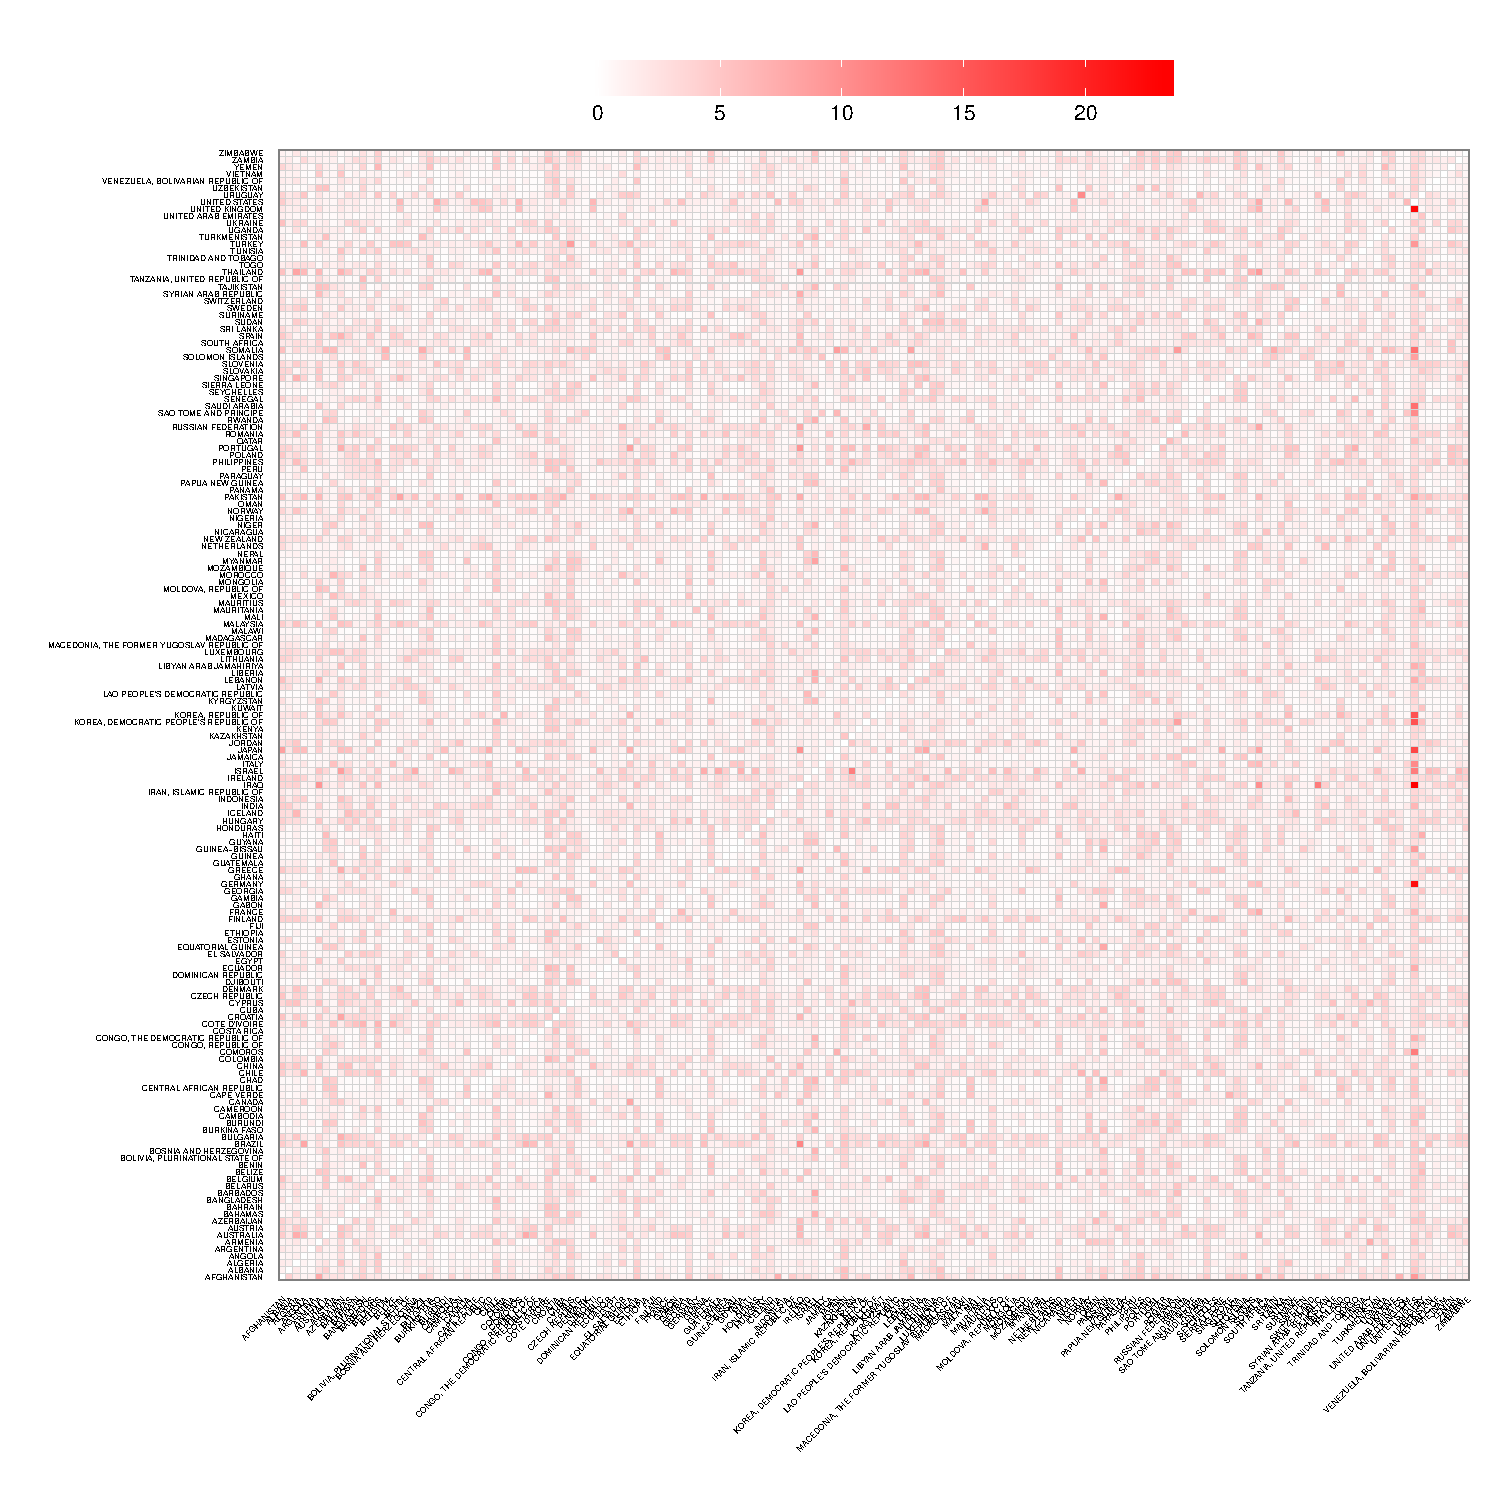
\includegraphics[width=.6\textwidth]{expiperf.pdf} & 
      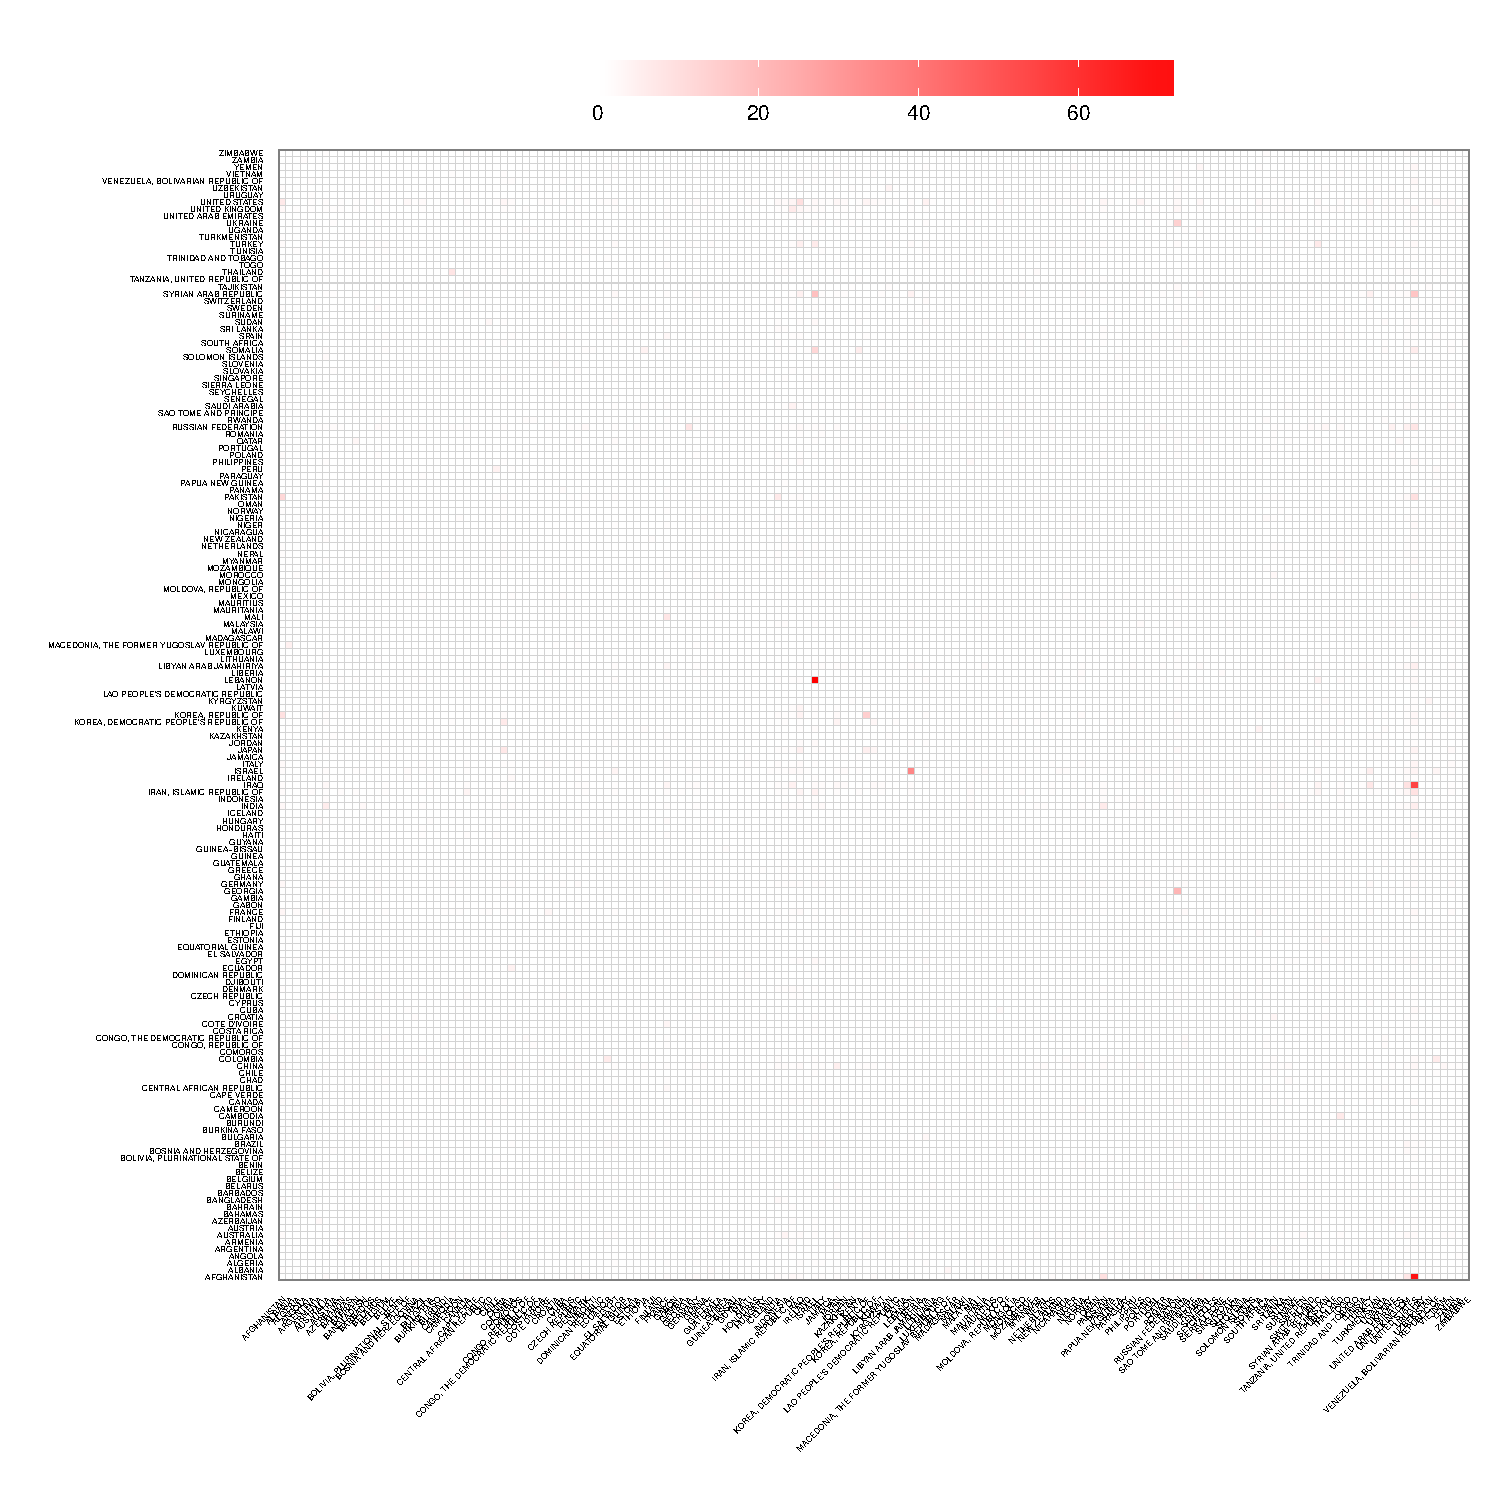
\includegraphics[width=.6\textwidth]{mconfiperf.pdf}
    \end{tabular}
  \end{figure}
}
%%%%%%%%%%%%%%%%%%%%%%%%%%%%%%%%%%%%%%%%%%%%%%%%%%%%%%%%%%%%

%%%%%%%%%%%%%%%%%%%%%%%%%%%%%%%%%%%%%%%%%%%%%%%%%%%%%%%%%%%%
\frame
{
\frametitle{Trace Plots for $\boldsymbol{\beta_{3}}$}
  \centering
  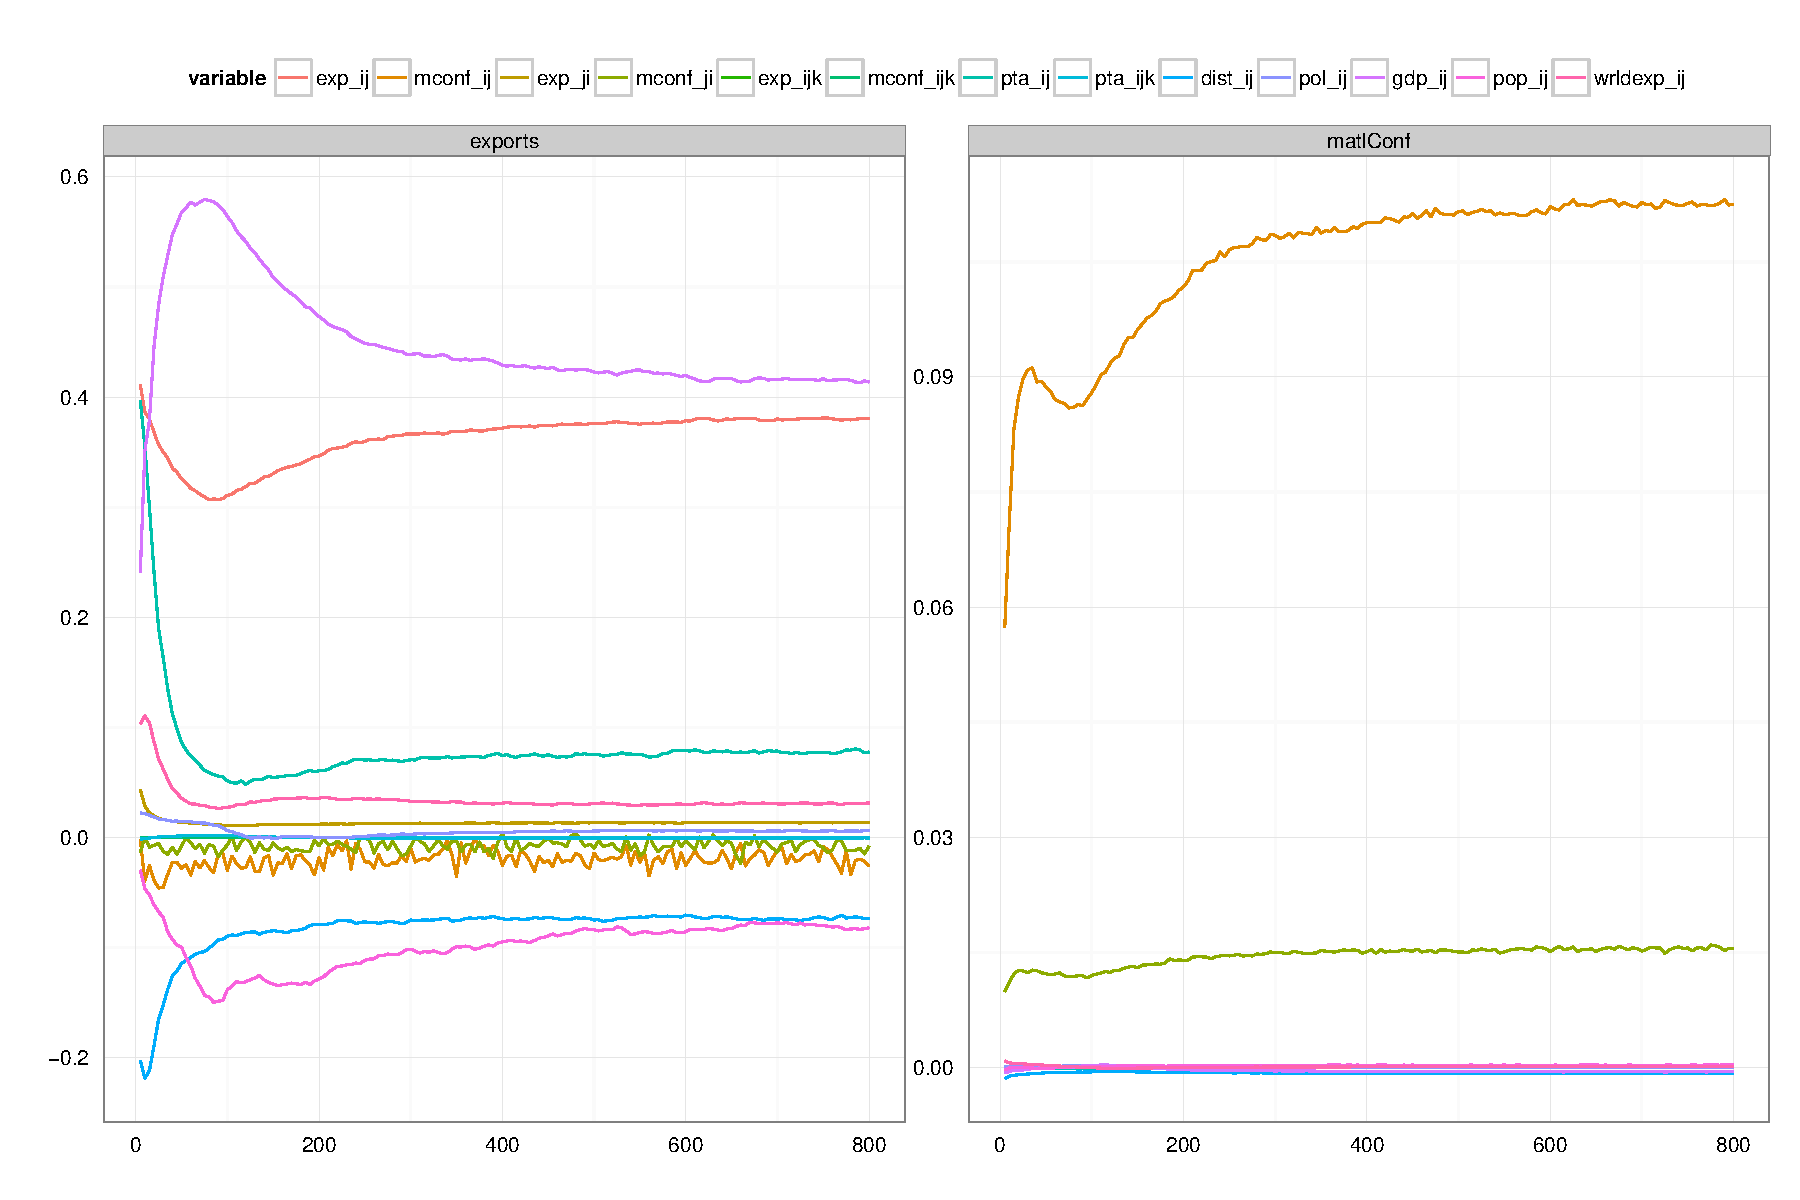
\includegraphics[width=1\textwidth]{trace.pdf}
}
%%%%%%%%%%%%%%%%%%%%%%%%%%%%%%%%%%%%%%%%%%%%%%%%%%%%%%%%%%%%

%%%%%%%%%%%%%%%%%%%%%%%%%%%%%%%%%%%%%%%%%%%%%%%%%%%%%%%%%%%%
\frame
{
  \frametitle{Comparison with directed dyadic model}
  \begin{itemize}
  \item Here I run a similar analysis using the standard directed dyadic (dd) framework
  \item The covariates for both models are the same 
  \item Instead of taking a vector autoregression approach, I just run two separate directed dyadic linear regressions
  \end{itemize}
} 
%%%%%%%%%%%%%%%%%%%%%%%%%%%%%%%%%%%%%%%%%%%%%%%%%%%%%%%%%%%%

%%%%%%%%%%%%%%%%%%%%%%%%%%%%%%%%%%%%%%%%%%%%%%%%%%%%%%%%%%%%
\frame
{
  \frametitle{dd Coefficient Results, std. errors in (), $^*$ sig. at $p< 0.05 $ }
  \vspace{-.3in}
  \tiny{\begin{table}[!ht]
\begin{tabular}{ l D{.}{.}{2}D{.}{.}{2} }

\hline 
  & \multicolumn{ 1 }{ c }{ Log(Exports) } & \multicolumn{ 1 }{ c }{ Std(Matl. Conf.) } \\ \hline

%                & Log(Exports)     & Std(Matl. Conf.)\\ 
exp\_ij         & 0.82 ^*          & -0.00 ^*        \\ 
                 & (0.00)           & (0.00)          \\ 
mconf\_ij       & -0.00            & 0.49 ^*         \\ 
                 & (0.00)           & (0.00)          \\ 
exp\_ji         & 0.06 ^*          & -0.00           \\ 
                 & (0.00)           & (0.00)          \\ 
mconf\_ji       & 0.00             & 0.03 ^*         \\ 
                 & (0.00)           & (0.00)          \\ 
exp\_ijk        & 0.00 ^*          & 0.00 ^*         \\ 
                 & (0.00)           & (0.00)          \\ 
mconf\_ijk      & -0.00 ^*         & 0.00 ^*         \\ 
                 & (0.00)           & (0.00)          \\ 
pta\_ij         & 0.10 ^*          & -0.00           \\ 
                 & (0.00)           & (0.00)          \\ 
pta\_ijk        & -0.00 ^*         & -0.00 ^*        \\ 
                 & (0.00)           & (0.00)          \\ 
dist\_ij        & -0.09 ^*         & -0.01 ^*        \\ 
                 & (0.00)           & (0.00)          \\ 
pol\_ij         & 0.01 ^*          & -0.00 ^*        \\ 
                 & (0.00)           & (0.00)          \\ 
gdp\_ij         & 0.13 ^*          & 0.01 ^*         \\ 
                 & (0.00)           & (0.00)          \\ 
pop\_ij         & -0.02 ^*         & 0.00 ^*         \\ 
                 & (0.00)           & (0.00)          \\ 
wrldexp\_ij     & 0.01 ^*          & -0.01 ^*        \\ 
                 & (0.00)           & (0.00)          
\\

$N$              & 4250400          & 4250400         \\ 
% $R^2$            & 0.89             & 0.26            \\ 
% adj. $R^2$       & 0.89             & 0.26            \\ 
% Resid. sd        & 2.37             & 0.86            
\\ \hline

% \multicolumn{3}{l}{\footnotesize{$^*$ indicates significance at $p< 0.05 $}}

\end{tabular}


\end{table}

}
}
%%%%%%%%%%%%%%%%%%%%%%%%%%%%%%%%%%%%%%%%%%%%%%%%%%%%%%%%%%%%

%%%%%%%%%%%%%%%%%%%%%%%%%%%%%%%%%%%%%%%%%%%%%%%%%%%%%%%%%%%%
\frame
{
  \frametitle{Parameter Estimate Comparisons: MLTR \& dd}
  \footnotesize{+ = sig at 95\% interval and positive} \\
  \footnotesize{--\; = sig at 95\% interval and negative}
  
  \centering
  \begin{tabular}{l | cc | cc}
~ & \multicolumn{2}{c}{Log(Exports)} & \multicolumn{2}{c}{Std(Matl. Conf.)} \\
\hline\hline
~ & MLTR & Dyadic & MLTR & Dyadic \\
\hline
  Log(Exports)$_{ij, t-1}$ & + & + & -- & -- \\
  Std(Matl. Conf.)$_{ij, t-1}$ & -- &  & + & + \\
  Log(Exports)$_{ji, t-1}$ & + & + & -- &  \\
  Std(Matl. Conf.)$_{ji, t-1}$ &  &  & + & + \\
  Log(Exports)$_{ijk, t-1}$ & + & + & + & + \\
  Std(Matl. Conf.)$_{ijk, t-1}$ &  & -- & + & -- \\
  PTAs$_{ij, t-1}$ & + & + & + &  \\
  PTAs$_{ijk, t-1}$ & -- & -- & -- & -- \\
  Distance$_{ij, t-1}$ & -- & -- & -- & -- \\
  Polity$_{i, t-1}$ & + & + & + & -- \\
  Log(GDP)$_{i, t-1}$ & + & + & -- & + \\
  Log(Population)$_{i, t-1}$ & -- & -- & + & + \\
  Log(Total~Exports)$_{i, t-1}$ & + & + & + & -- 
  \end{tabular}
}
%%%%%%%%%%%%%%%%%%%%%%%%%%%%%%%%%%%%%%%%%%%%%%%%%%%%%%%%%%%%

%%%%%%%%%%%%%%%%%%%%%%%%%%%%%%%%%%%%%%%%%%%%%%%%%%%%%%%%%%%%
\frame
{
\frametitle{DD Aggregate Performance \& RMSE by i-j}
  % latex table generated in R 3.1.2 by xtable 1.7-4 package
% Mon Jun 29 07:11:33 2015
\begin{table}[ht]
\centering
\begin{tabular}{rrr}
  \hline
 & RMSE & R$^{2}$ \\ 
  \hline
Log(Exports) & 2.37 & 0.89 \\ 
  Std(Matl. Conf.) & 0.86 & 0.26 \\ 
   \hline
\end{tabular}
\end{table}

  \begin{figure}[ht]
  \centering
    \begin{tabular}{cc}
      \hspace*{-.63in}
      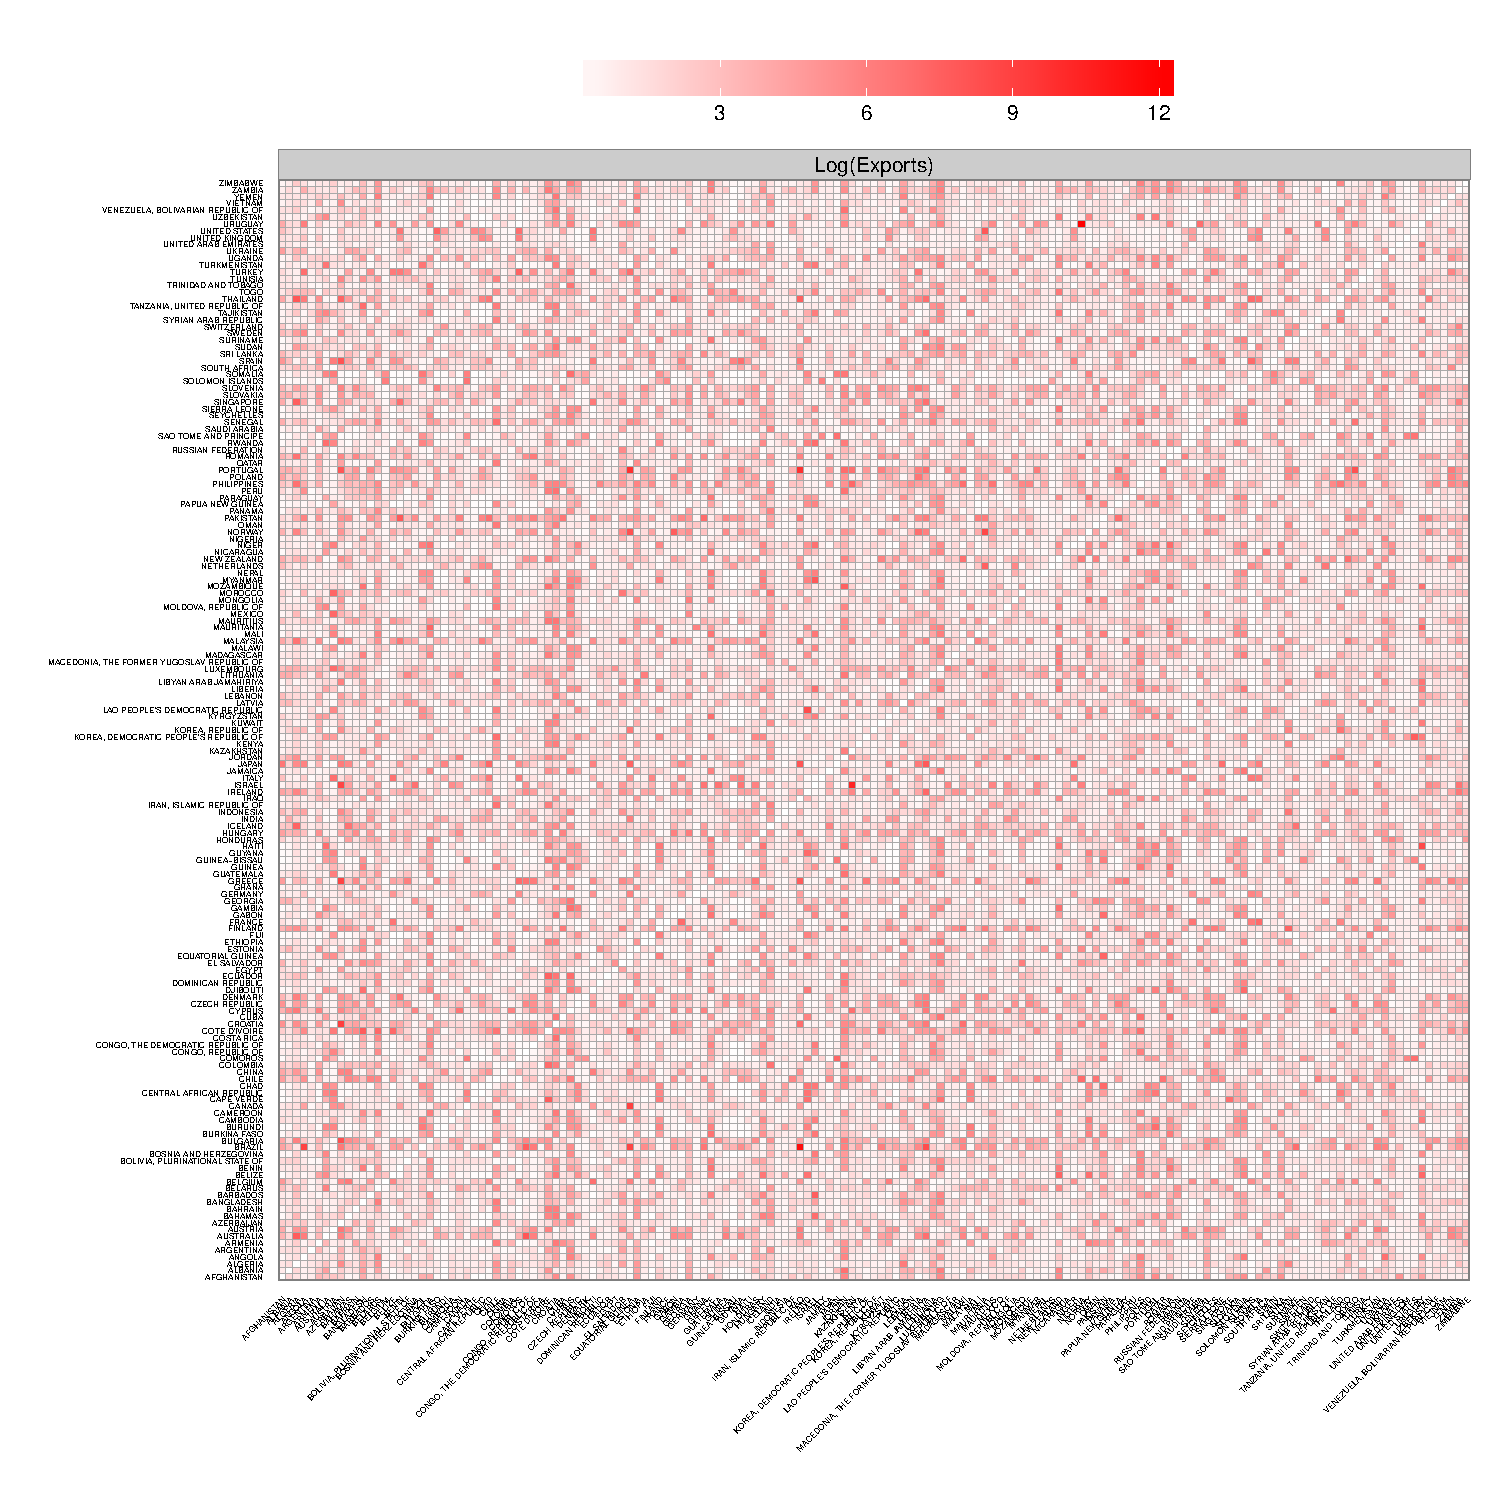
\includegraphics[width=.6\textwidth]{dyadexpiperf.pdf} & 
      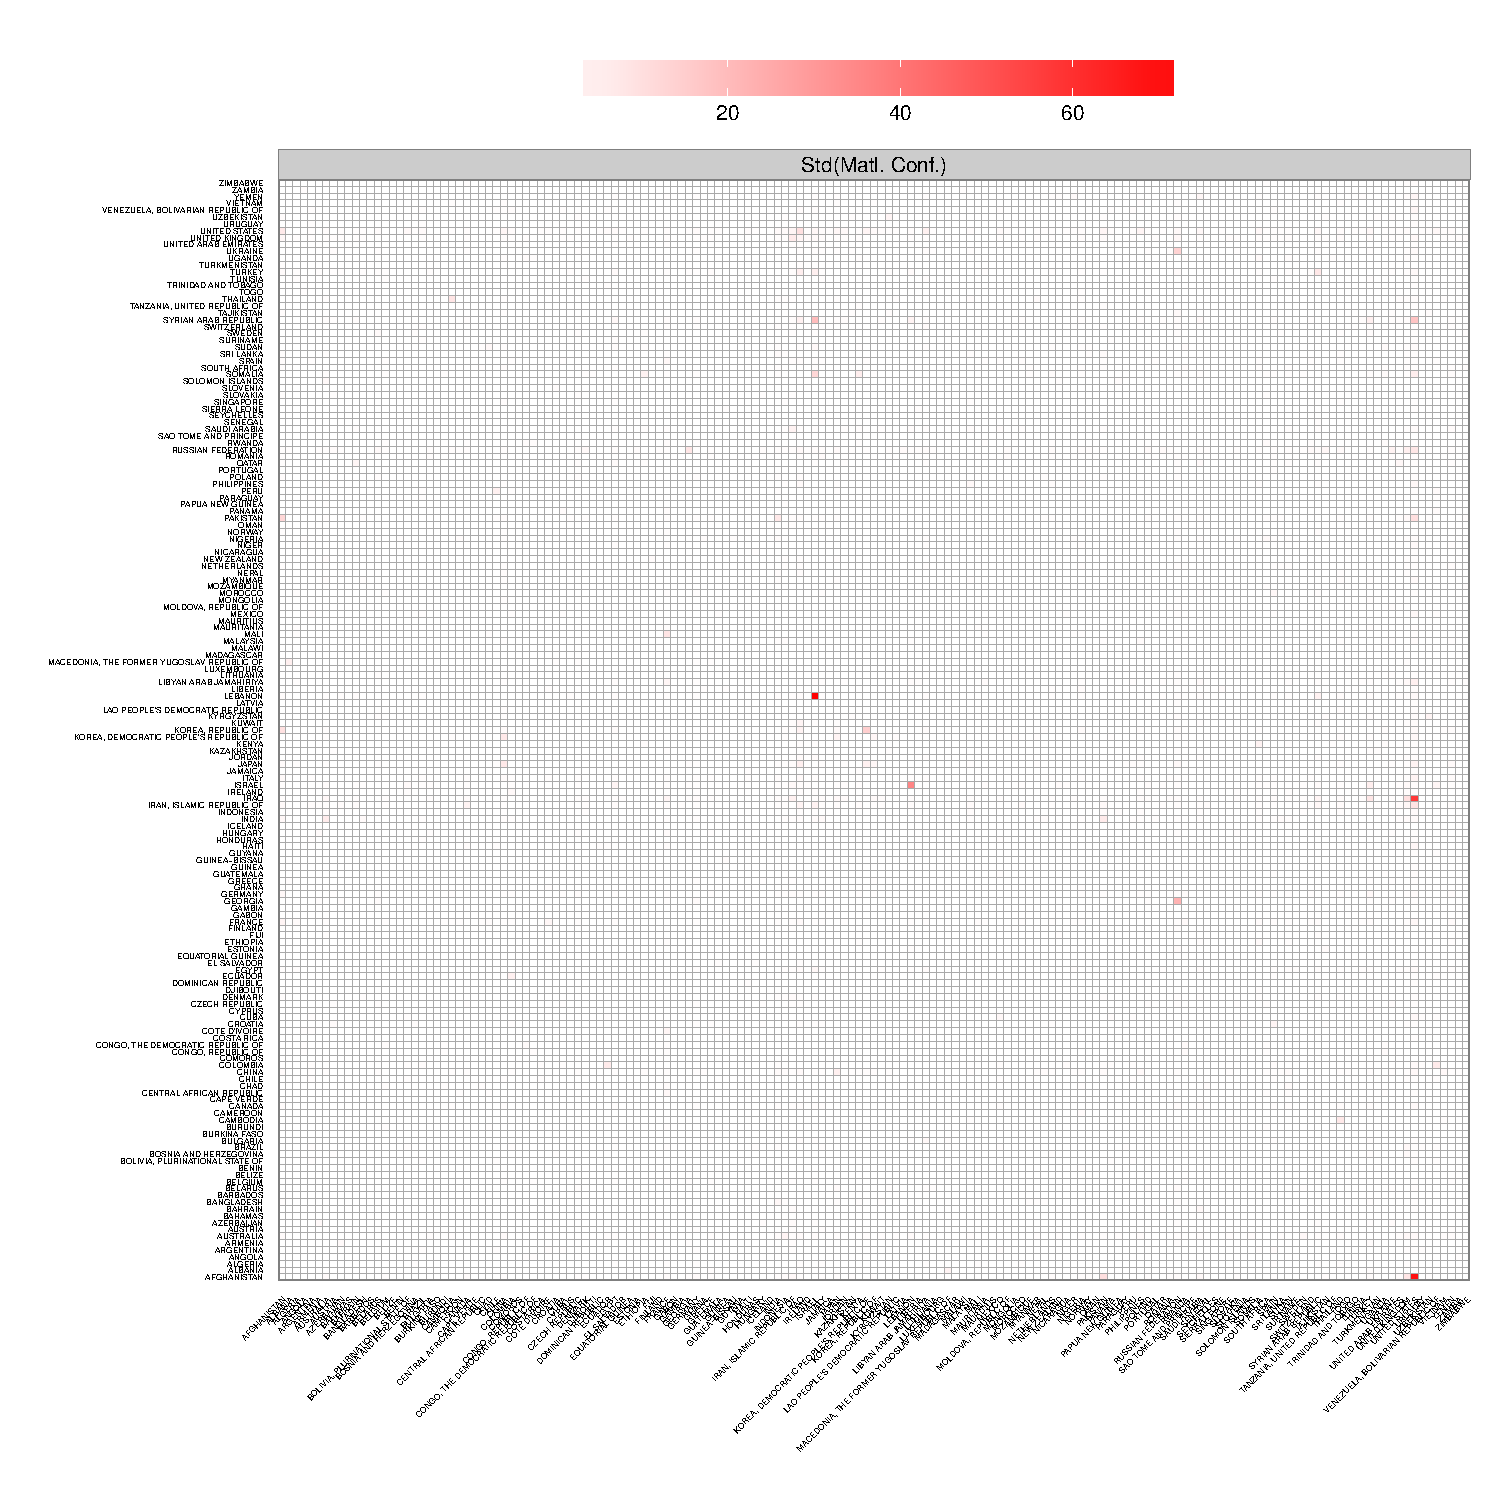
\includegraphics[width=.6\textwidth]{dyadmconfiperf.pdf}
    \end{tabular}
  \end{figure}
}
%%%%%%%%%%%%%%%%%%%%%%%%%%%%%%%%%%%%%%%%%%%%%%%%%%%%%%%%%%%%

%%%%%%%%%%%%%%%%%%%%%%%%%%%%%%%%%%%%%%%%%%%%%%%%%%%%%%%%%%%%
\frame
{
  \frametitle{Performance Comparisons: MLTR \& DD}

\begin{itemize}
\item Across all cases the R$^{2}$ is higher using the MLTR approach for both exports (95\% v. 89\%) and matl. conf. (28\% v. 26\%)
\item MLTR has a lower RMSE in $\approx$ 57\% of cases for Log(Exports)
\item MLTR has a lower RMSE in $\approx$ 80\% of cases for Std(Matl. Conf.)
\item Across all cases the RMSE is lower using the MLTR approach for both exports (2.32 v. 2.37) and matl. conf. (0.85 v. 0.86)
\item However, as shown by the aggregate RMSE statistics right above, the differences in performance are small
\item Additionally, in the next two slides I break out the performance, in terms of RMSE, by showing the results for OECD--OECD and Not OECD--Not OECD countries
\end{itemize}

}
%%%%%%%%%%%%%%%%%%%%%%%%%%%%%%%%%%%%%%%%%%%%%%%%%%%%%%%%%%%%

%%%%%%%%%%%%%%%%%%%%%%%%%%%%%%%%%%%%%%%%%%%%%%%%%%%%%%%%%%%%
\frame
{
  \frametitle{Performance on OECD--OECD countries: Log(Exports)}
  \centering
  \includegraphics[width=1\textwidth]{oecdexpiperf.pdf}
}
%%%%%%%%%%%%%%%%%%%%%%%%%%%%%%%%%%%%%%%%%%%%%%%%%%%%%%%%%%%%

%%%%%%%%%%%%%%%%%%%%%%%%%%%%%%%%%%%%%%%%%%%%%%%%%%%%%%%%%%%%
\frame
{
  \frametitle{Performance on OECD--OECD countries: Std(Matl. Conf.)}
  \centering
  \includegraphics[width=1\textwidth]{oecdconfiperf.pdf}
}
%%%%%%%%%%%%%%%%%%%%%%%%%%%%%%%%%%%%%%%%%%%%%%%%%%%%%%%%%%%%

\plain{Next Steps?}

\end{document}
